% Chapter 7 source: maintained directly in LaTeX; diagrams have editable sources in Diagrams/.
\section{Thiết kế hệ thống}
\label{sec:system-design}
\setcounter{paragraph}{0}

Chương này trình bày thiết kế đề xuất cho hai hệ thống độc lập Wispace và AIHub, mỗi hệ thống có frontend React và backend .NET riêng. Wispace là sản phẩm chính, cung cấp môi trường luyện tập, thi thử và theo dõi tiến bộ IELTS cho người học. AIHub cung cấp cổng quản lý và khai thác API mô hình cho khách hàng doanh nghiệp, đồng thời có các công cụ nội bộ phục vụ đánh giá và cải thiện chất lượng mô hình.

Wispace sử dụng kiến trúc microservices theo các nhóm nghiệp vụ chính, hướng tới 1.000--10.000 người luyện tập hoặc thi đồng thời. AIHub giữ backend modular monolith riêng cho B2B và công cụ nội bộ. Các dịch vụ .NET của Wispace, hệ thống AIHub và Python FastAPI có hợp đồng tích hợp, quyền truy cập và tài nguyên được kiểm soát độc lập; Wispace gọi dịch vụ chấm trực tiếp qua Assessment, không qua cổng B2B.

Nội dung chương bao gồm kiến trúc tổng thể, phân chia module, thiết kế dữ liệu, xử lý âm thanh và chấm bài, quản lý API B2B, bảo mật, triển khai và giám sát. Thiết kế giữ giả định Scoring Model do Wispace tự huấn luyện; trọng tâm của chương là tích hợp và vận hành mô hình trong hệ thống. Các chỉ tiêu hiệu năng và độ chính xác là mục tiêu cần kiểm chứng khi hiện thực và thực nghiệm.

\subsection{Thiết kế hệ thống Wispace}

\subsubsection{Phạm vi, giao diện và kiến trúc}

Wispace là hệ thống học tập chính, tập trung vào luyện tập và thi thử Speaking IELTS. Thiết kế tách Core, Learning \& Exam, Assessment, Progress \& Reporting và AI Inference thành các đơn vị triển khai độc lập. Các dịch vụ nghiệp vụ dùng ASP.NET Core; AI Inference dùng Python FastAPI và Scoring Model tự huấn luyện. API Gateway định tuyến yêu cầu từ React; dịch vụ kiểm tra quyền nghiệp vụ tại ranh giới dữ liệu của mình. Mỗi dịch vụ có thể tổ chức nội bộ theo module, nhưng không dùng chung bảng dữ liệu với dịch vụ khác \cite{ch7_microservices,ch7_microservices_data}.

Phần thiết kế này bao gồm tài khoản, kho đề, kiểm duyệt, phiên luyện tập/thi thử, ghi âm, chấm điểm, báo cáo, lộ trình và quyền lợi gói học. Các chức năng AIHub được trình bày riêng tại Mục 7.2; việc dùng chung hạ tầng không làm hợp nhất hai phạm vi nghiệp vụ.

\paragraph*{Tổ chức frontend}

Frontend Wispace được tổ chức thành các nhóm màn hình tài khoản, kho đề, phòng luyện tập, phòng thi thử, kết quả, tiến bộ và quản trị nội dung. Các thành phần ghi âm, bộ đếm thời gian và trình phát audio được đóng gói để dùng chung giữa luyện tập và thi thử, nhưng quy tắc thao tác của hai chế độ được xử lý riêng.

Trong chế độ luyện tập, học viên có thể nghe lại và ghi lại trước khi nộp. Trong chế độ thi thử, hệ thống sử dụng trạng thái phiên trên backend để xác định Part, câu hỏi và thời hạn. Thời gian trên trình duyệt chỉ phục vụ hiển thị; mốc thời gian do backend lưu là căn cứ khi khôi phục phiên hoặc kết thúc bài.

Audio được thu theo khả năng trình duyệt. WebM/Opus và MP4/AAC là các đầu vào cần được hỗ trợ theo yêu cầu. FastAPI chuẩn hóa audio về định dạng đầu vào của Scoring Model; ứng dụng không giả định trình duyệt luôn ghi được đúng 16 kHz chỉ dựa vào tham số yêu cầu của MediaRecorder.

Để khôi phục khi mạng chập chờn, các đoạn ghi được lưu tạm trong IndexedDB và đánh số thứ tự. Mỗi đoạn có \texttt{upload\allowbreak{}Session\allowbreak{}Id}, \texttt{part\allowbreak{}Number} và checksum. Learning cấp URL tải lên có thời hạn để React gửi từng đoạn trực tiếp tới Object Storage; đường truyền audio không đi xuyên các API nghiệp vụ. Sau khi Learning xác minh object và checksum, frontend mới đánh dấu đoạn đó hoàn tất. Khi kết thúc, Learning kiểm tra manifest các đoạn, thứ tự và kích thước trước khi chấp nhận bài chấm.

\begin{figure}[H]
\centering
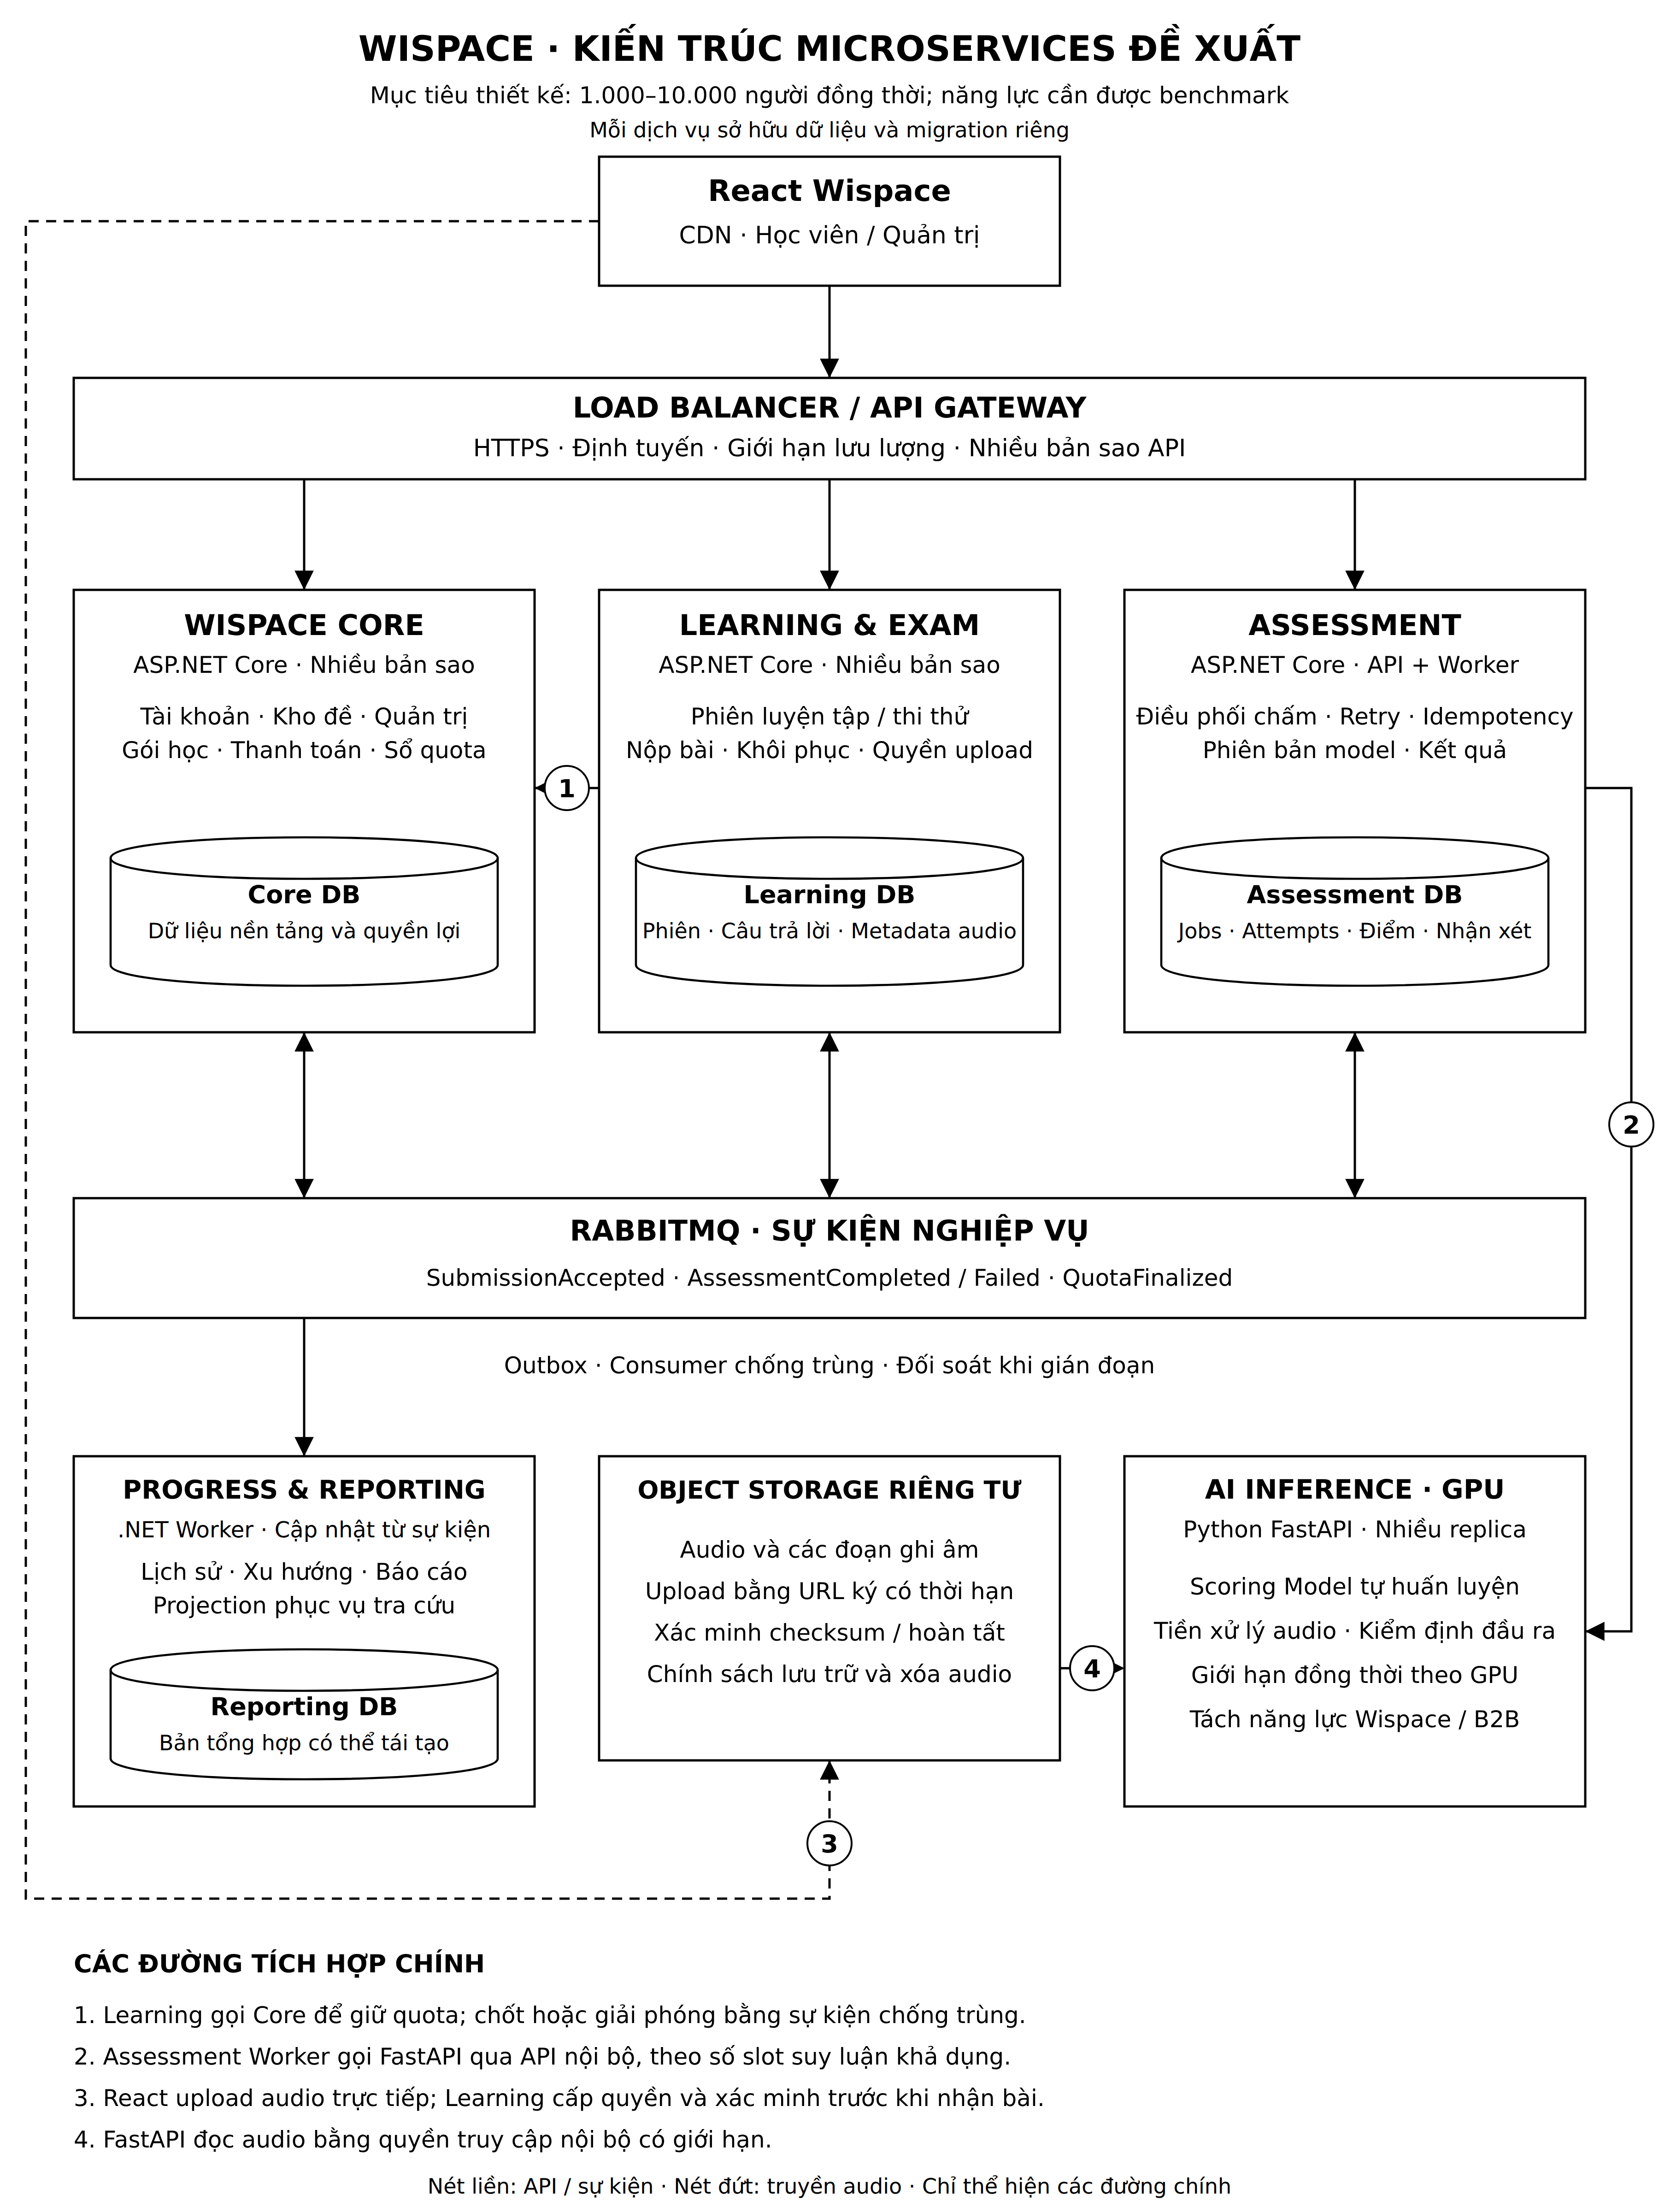
\includegraphics[width=\linewidth,height=.72\textheight,keepaspectratio]{Images/Design/wispace_microservices_proposal.png}
\caption{Kiến trúc microservices đề xuất cho Wispace}
\label{design:fig:wispace_architecture}
\end{figure}

\clearpage
\paragraph*{Ranh giới dịch vụ và quyền sở hữu dữ liệu}

\begingroup\small\setstretch{1.1}
\begin{longtable}{|>{\raggedright\arraybackslash}p{.25\linewidth}|>{\raggedright\arraybackslash}p{.65\linewidth}|}
\caption{Các dịch vụ của Wispace}\label{design:tab:1}\\\hline
\textbf{Dịch vụ} & \textbf{Trách nhiệm và dữ liệu sở hữu} \\\hline
\endfirsthead
\hline\textbf{Dịch vụ} & \textbf{Trách nhiệm và dữ liệu sở hữu} \\\hline\endhead
Core & Tài khoản, phiên đăng nhập, kho đề, kiểm duyệt, gói học, thanh toán và sổ quota. Core DB lưu danh tính, đề có phiên bản, giao dịch và bút toán quyền lợi. \\\hline
Learning \& Exam & Phiên học/thi, thời hạn máy chủ, câu trả lời, manifest audio và tiếp nhận bài nộp. Learning DB lưu trạng thái phiên và submission; dịch vụ cấp quyền upload sau khi kiểm tra chủ sở hữu. \\\hline
Assessment & API trạng thái/kết quả và Worker điều phối chấm. Assessment DB sở hữu job, attempt, lease, phiên bản mô hình, kết quả, báo cáo thi thử và liên kết chia sẻ. \\\hline
Progress \& Reporting & API đọc và Worker tổng hợp lịch sử, xu hướng, lỗi lặp và roadmap. Reporting DB là bản tổng hợp từ sự kiện, có thể tái tạo từ nguồn dữ liệu nghiệp vụ. \\\hline
AI Inference & FastAPI nạp Scoring Model, chuẩn hóa audio, suy luận và kiểm định đầu ra. Không sửa dữ liệu bài làm hoặc sổ quota; kết quả được Assessment công nhận và lưu. \\\hline
\end{longtable}\endgroup

Không tách một service cho từng bảng CRUD. Core giữ các nghiệp vụ nền tảng trong một lõi có module; phiên thi, điều phối chấm, báo cáo và suy luận được tách để mở rộng và phát hành độc lập. Các dịch vụ gọi Core qua hợp đồng API cho nghiệp vụ giữ quota, không truy vấn trực tiếp Core DB. Nội dung đề được Core cung cấp với phiên bản; Learning lưu snapshot câu hỏi của phiên để thay đổi kho đề không sửa lịch sử thi.

\paragraph*{Mục tiêu tải và nguyên tắc cô lập}

Mức 1.000--10.000 người đồng thời là mục tiêu thiết kế cần kiểm chứng, không phải kết quả đo. Phải phân biệt người đang mở trang, đang ghi âm, đang upload, bài nộp mỗi giây và lượt suy luận đang chạy. Nếu 10.000 người đều tải một đoạn audio mỗi 5 giây, lưu lượng trung bình riêng đường upload là khoảng 2.000 yêu cầu/giây; đây là kịch bản tính toán, chưa phải benchmark. Thiết kế sử dụng upload trực tiếp, nhiều bản sao API, cache nội dung đề và hàng đợi có giới hạn để phân tách các nhóm tải.

Luồng chuyển câu trong thi thử không đợi chấm câu trước. Learning quyết định câu và thời hạn từ trạng thái phiên; TTS được chuẩn bị hoặc cache trước. Lỗi Assessment hoặc GPU không được làm mất các đoạn audio đã xác nhận hoặc ngăn tiếp tục phiên thi đủ điều kiện. Trạng thái phiên cần lưu bền vững, không chỉ nằm trong bộ nhớ của một replica.

\subsubsection{Thiết kế dữ liệu và audio}

\begin{figure}[H]
\centering
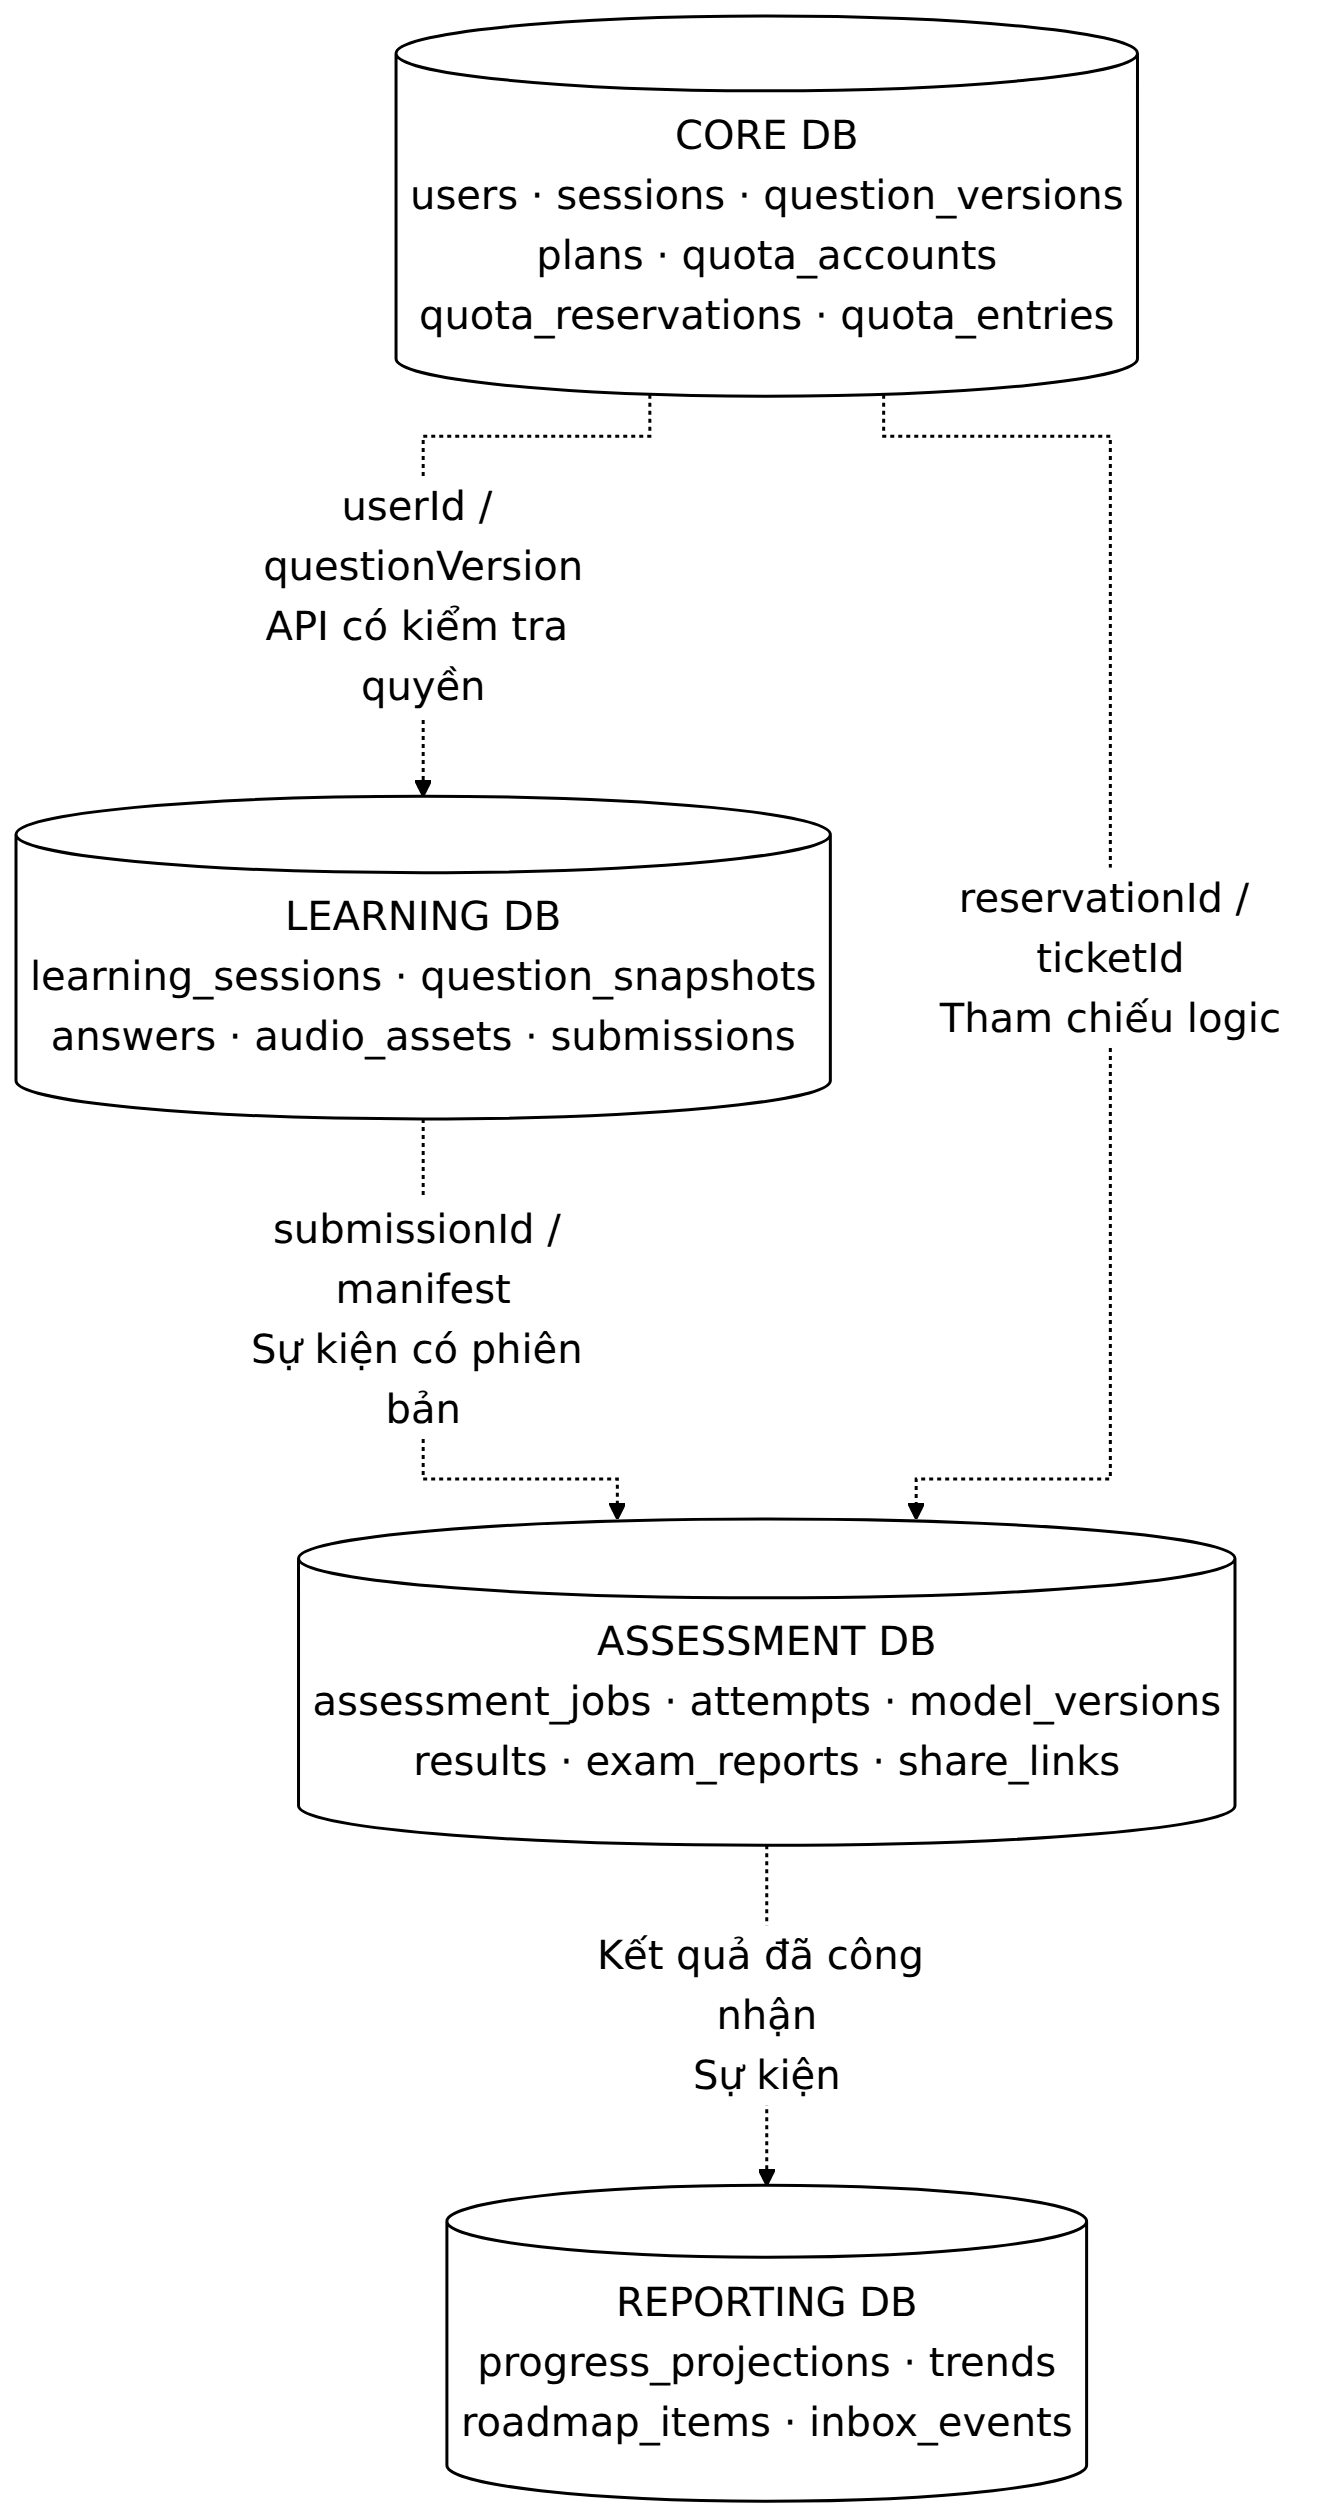
\includegraphics[width=\linewidth,height=.72\textheight,keepaspectratio]{Images/Design/wispace_data.png}
\caption{Phân tách dữ liệu theo dịch vụ Wispace}
\label{design:fig:wispace_data}
\end{figure}

Sơ đồ thể hiện quyền sở hữu dữ liệu theo dịch vụ. Mỗi dịch vụ nghiệp vụ có PostgreSQL database, credentials và migration riêng; các database có thể đặt cùng cụm vật lý khi năng lực cho phép. Các mã người học, phiên, submission và reservation được truyền qua API/sự kiện. Liên kết xuyên dịch vụ là định danh logic, không phải khóa ngoại hoặc transaction xuyên database. Một submission có thể có nhiều job do chấm lại; mỗi job có nhiều attempt và tối đa một kết quả cuối cùng được công nhận. Reporting chỉ lưu bản tổng hợp, không trở thành nguồn quyết định quota hoặc trạng thái thi.

PostgreSQL lưu metadata, object key, checksum, kích thước và trạng thái; nội dung audio nằm trong bucket riêng tư. Object key được backend tạo theo định danh nội bộ và không sử dụng tên tệp do người dùng gửi làm đường dẫn lưu trữ.

Learning chỉ cấp quyền tải lên cho object thuộc phiên và câu trả lời mà người dùng sở hữu. Việc hoàn tất upload phải kiểm tra object thực tế, checksum và giới hạn kích thước trước khi đánh dấu \texttt{Uploaded}. Link tải lên không đồng nghĩa tệp đã được chấp nhận để chấm.

Khi người dùng nghe lại bài, backend kiểm tra quyền và cấp URL đọc có thời hạn tối đa 10 phút theo yêu cầu đã xác định. URL ký trước là quyền truy cập tạm thời vào đúng object; hệ thống không ghi toàn bộ URL vào log \cite{ch7_s3_presigned}. Với Assessment Worker, quyền đọc object được lấy từ dịch vụ Learning hoặc tài khoản dịch vụ có phạm vi tương ứng tại thời điểm bắt đầu từng attempt, tránh hết hạn khi chờ hàng đợi. Message chỉ mang object key và metadata đã xác minh; không chứa audio hoặc URL ký dài hạn.

Tác vụ định kỳ xóa audio sau 180 ngày theo chính sách ở Chương 5, cập nhật trạng thái tệp và giữ transcript, điểm cùng các dữ liệu được phép lưu. Yêu cầu xóa trước hạn cũng được đưa vào quy trình có thể thử lại. Dữ liệu trong bản sao lưu tuân theo vòng đời backup được công bố; thời điểm xóa khỏi hệ thống hoạt động không được mô tả như xóa tức thời khỏi mọi bản sao lưu.

\subsubsection{Thiết kế tích hợp AI và xử lý bài làm}

\paragraph*{Tiếp nhận bài, quota và nhất quán xuyên dịch vụ}

Learning tạo submission ở trạng thái chờ, gắn khóa chống trùng và tham chiếu audio đã xác minh. Learning gọi Core để giữ quota bằng cùng mã nghiệp vụ; Core kiểm tra quyền lợi và ghi reservation trong transaction của Core DB. Khi được xác nhận, Learning ghi trạng thái Accepted và sự kiện \texttt{Submission\allowbreak{}Accepted} vào outbox trong cùng transaction của Learning DB, sau đó trả \texttt{202 Accepted} cùng \texttt{submission\allowbreak{}Id} và URL trạng thái. Assessment nhận sự kiện, tạo job và outbox xử lý trong transaction của Assessment DB; job được ràng buộc duy nhất theo submission và loại lần chấm.

Đây là chuỗi giao dịch cục bộ có bù và đối soát, không phải một transaction ACID bao trùm bốn database. Nếu lời gọi giữ quota timeout, Learning tra cứu kết quả bằng cùng mã nghiệp vụ trước khi tiếp tục hoặc hủy. Nếu Core đã giữ quota nhưng Learning chưa Accepted, tác vụ đối soát phục hồi hoặc dùng cập nhật có điều kiện để xác nhận hủy submission tại Learning trước khi Core giải phóng phần giữ đúng một lần. Khi trạng thái phía Learning chưa xác định, không tự hoàn quota chỉ vì timeout. Submission đã Accepted phải được giao nhận lại từ outbox hoặc đối soát cho tới khi Assessment ghi nhận; việc hết hạn không được âm thầm xóa bài đã nhận.

\begin{figure}[H]\centering
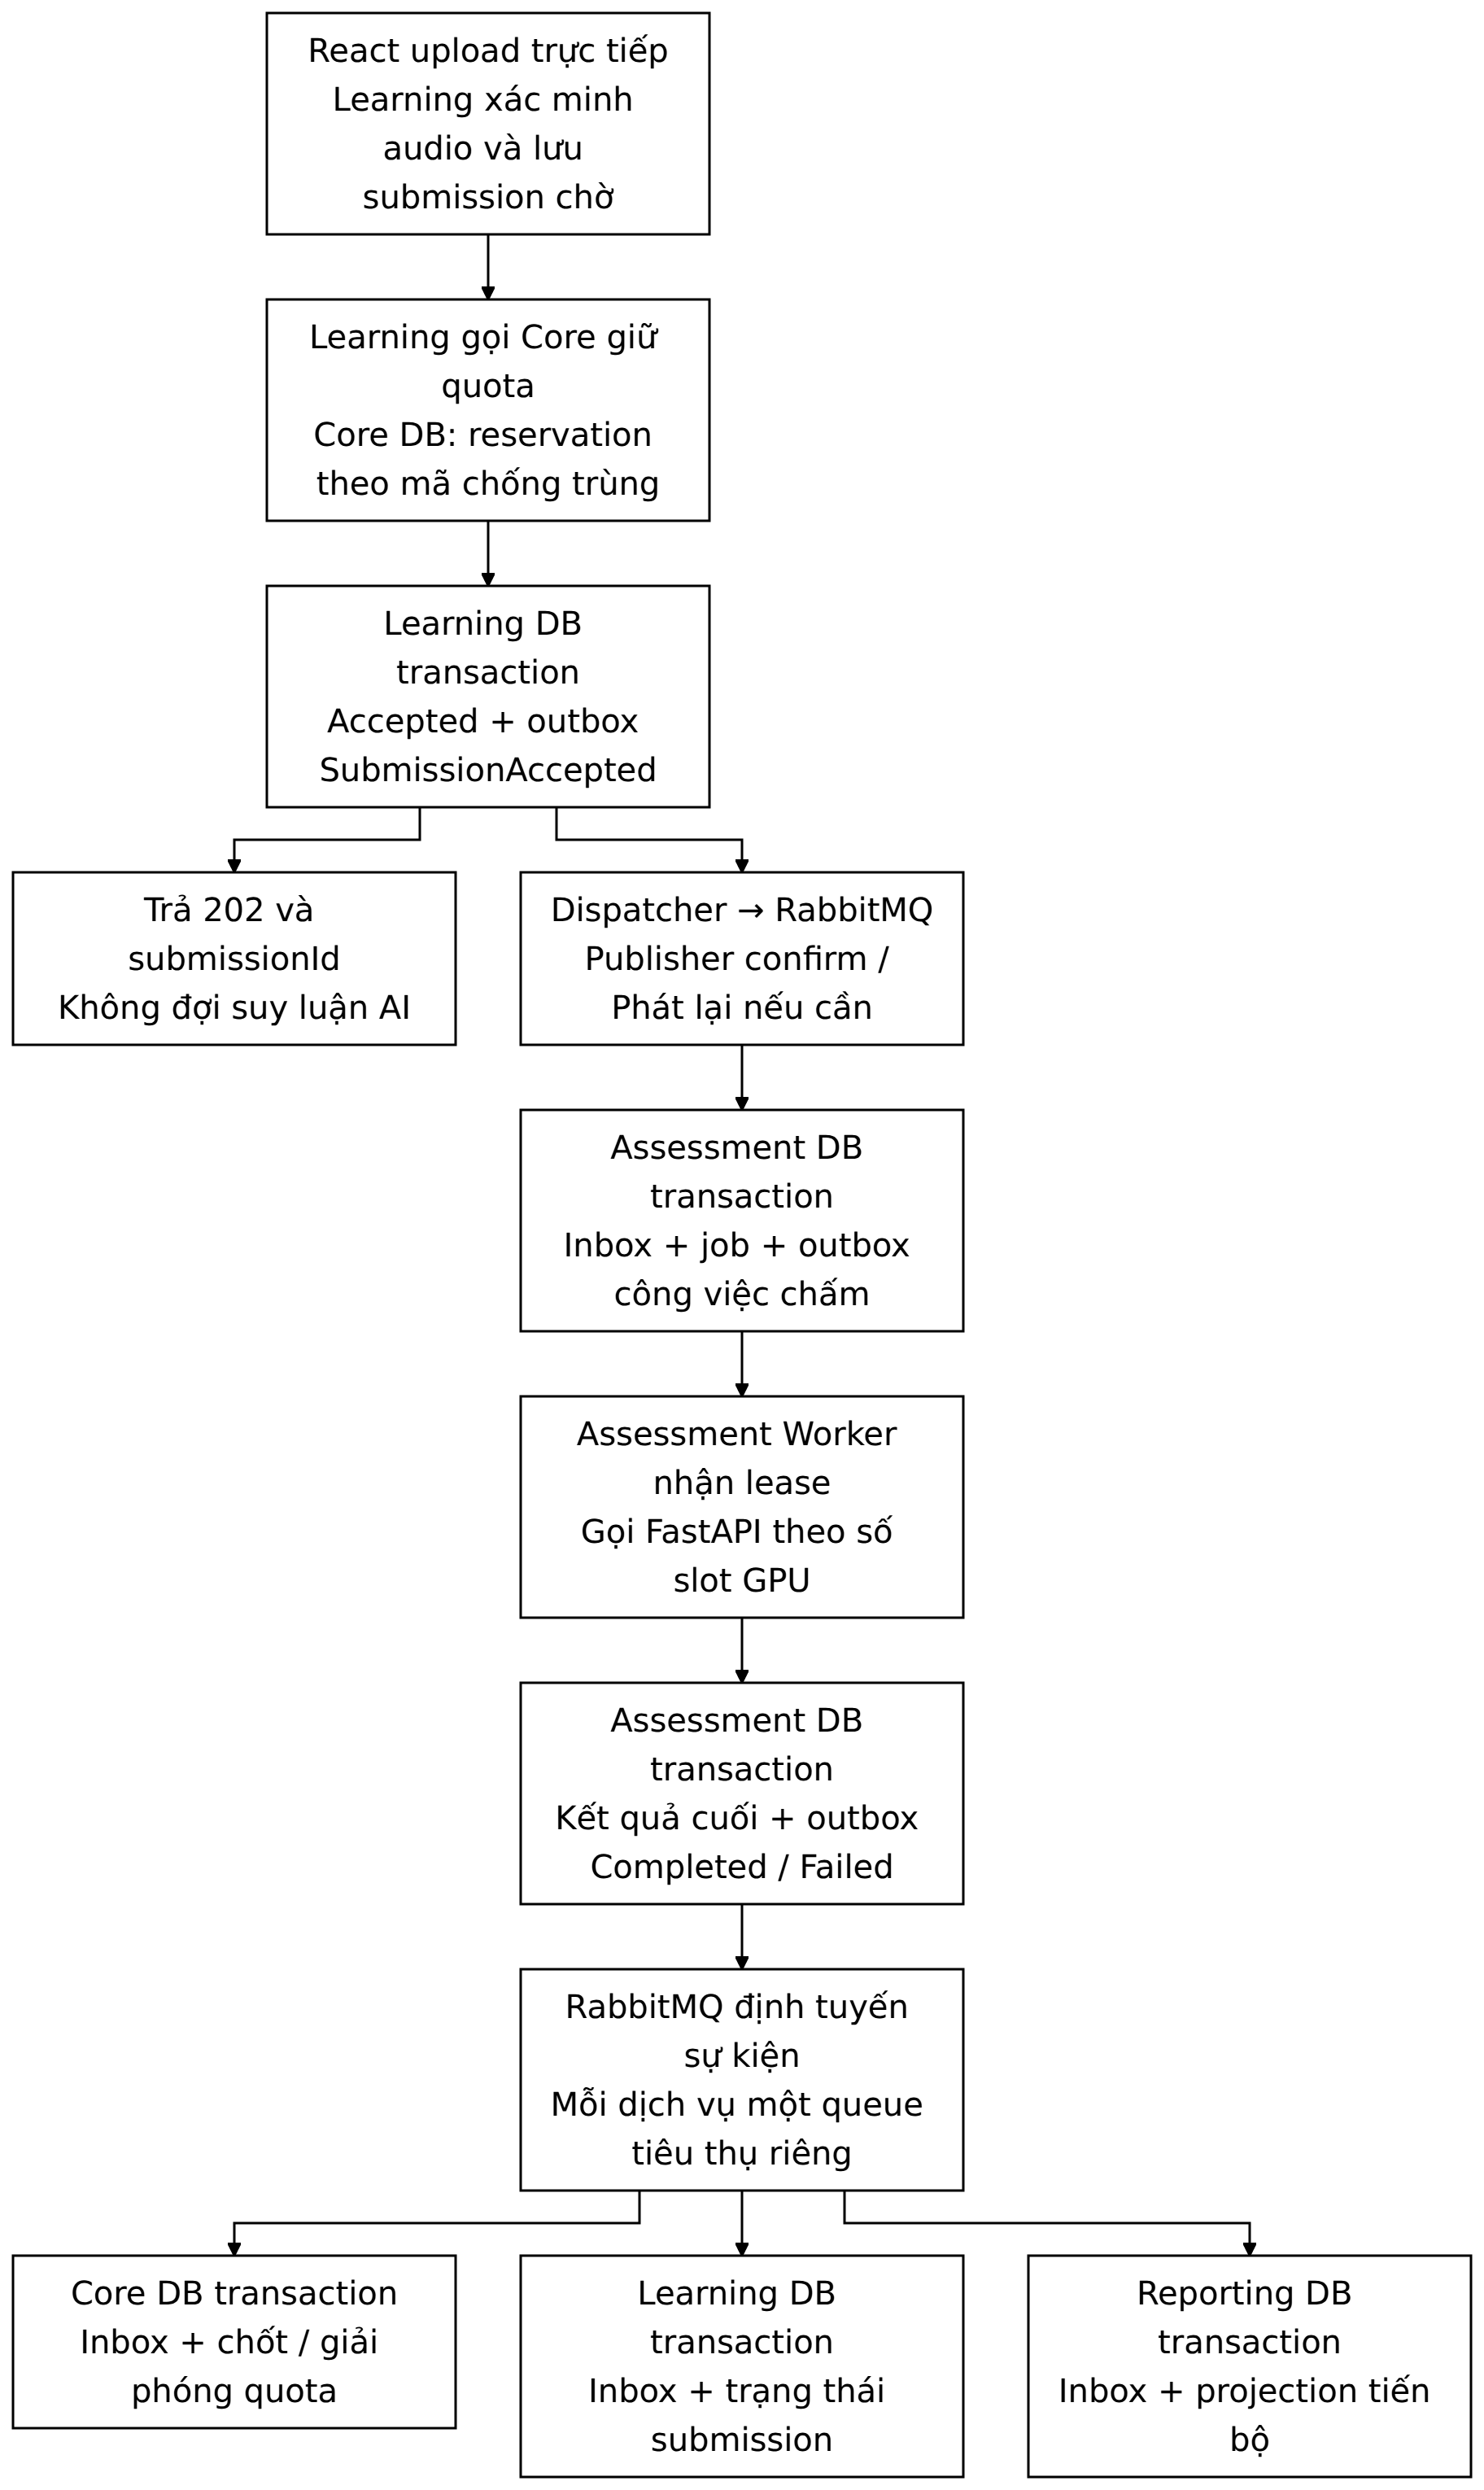
\includegraphics[width=\linewidth,height=.72\textheight,keepaspectratio]{Images/Design/speaking_flow.png}
\caption{Luồng chấm Speaking và giao dịch cục bộ giữa các dịch vụ}
\label{design:fig:speaking_flow}\end{figure}

\begingroup\emergencystretch=2em
Assessment lưu kết quả cuối cùng và sự kiện \texttt{Assessment\allowbreak{}Completed} hoặc \texttt{Assessment\allowbreak{}Failed} trong cùng transaction của Assessment DB. Core tiêu thụ sự kiện để chốt hoặc giải phóng reservation trong Core DB, chống trùng theo \texttt{event\allowbreak{}Id} và mã nghiệp vụ; Learning cập nhật trạng thái bài, Reporting cập nhật bản tổng hợp bằng các queue riêng. Trạng thái chấm xong và trạng thái đối soát quota có thể đến khác thời điểm; UI không biến độ trễ sự kiện thành yêu cầu nộp hoặc tính phí mới.
\par\endgroup

\paragraph*{Lựa chọn RabbitMQ và hợp đồng sự kiện}

RabbitMQ được dùng cho phân phối việc chấm và trao đổi sự kiện nghiệp vụ, phù hợp với nhu cầu chia công việc cho các Worker \cite{ch7_rabbitmq_workqueues}. Hai mục đích có queue riêng: một công việc chỉ cần một Worker xử lý tại một thời điểm, còn sự kiện kết quả được định tuyến vào các queue riêng của Core, Learning và Reporting để mỗi bên đều nhận được. Các consumer trong cùng một queue cạnh tranh công việc; không dùng chung queue cho ba bên với kỳ vọng mỗi bên đều nhận mọi sự kiện.

Thiết kế dùng durable queue, persistent message và publisher confirms; triển khai production chọn quorum queue có các replica trên các node độc lập phù hợp cấu hình cluster. Dispatcher chỉ đánh dấu đã phát khi nhận confirm và xử lý trường hợp message không định tuyến được. Consumer dùng manual acknowledgement sau khi transaction cục bộ hoàn tất; inbox lưu \texttt{event\allowbreak{}Id} trong cùng transaction với hiệu ứng nghiệp vụ để chống xử lý trùng \cite{ch7_rabbitmq_confirms,ch7_rabbitmq_quorum}.

\begingroup\emergencystretch=2em
Mỗi sự kiện có \texttt{event\allowbreak{}Id}, \texttt{event\allowbreak{}Type}, \texttt{schema\allowbreak{}Version}, \texttt{occurred\allowbreak{}At}, traceId, \texttt{aggregate\allowbreak{}Id} và \texttt{aggregate\allowbreak{}Version}, cùng các định danh submission, job, user và reservation cần thiết. Consumer kiểm tra phiên bản và trạng thái chuyển tiếp, xử lý sự kiện đến trễ hoặc trùng; không giả định thứ tự toàn cục giữa các queue. Retry có backoff và dead-letter queue, không requeue vô hạn. Timeout acknowledgement và lease được cấu hình phù hợp thời hạn thực thi; giám sát cả message chưa ack để tránh giữ việc trên Worker đã lỗi. Không đưa audio, secret hoặc URL riêng tư dài hạn vào sự kiện. Bản tổng hợp được tái tạo từ snapshot có mốc phiên bản qua API xuất dữ liệu có kiểm soát của Assessment, rồi áp dụng sự kiện tiếp theo bằng khóa chống trùng. RabbitMQ không được dùng làm kho lịch sử duy nhất: dữ liệu nghiệp vụ và outbox được lưu theo chính sách để đối soát hoặc xây dựng lại projection. Kafka chưa nằm trong phạm vi triển khai này.
\par\endgroup

\paragraph*{Thực thi và khả năng khôi phục}

Worker nhận thông điệp chỉ chứa định danh cần thiết như \texttt{job\allowbreak{}Id}, \texttt{source}, \texttt{trace\allowbreak{}Id} và phiên bản hợp đồng. Audio không được đặt trực tiếp trong thông điệp. Trước khi gọi AI, Worker đọc lại trạng thái job và giành quyền thực thi bằng cập nhật có điều kiện, kèm lease và số thứ tự lần thực thi.

Mỗi lần xử lý có \texttt{attempt\allowbreak{}Id} riêng. Kết quả chỉ được chấp nhận nếu attempt vẫn là chủ sở hữu hợp lệ của job. Một tác vụ theo dõi phát hiện lease hết hạn để đưa công việc về diện cần khôi phục. Cách này hạn chế việc Worker cũ trả kết quả muộn sau khi một Worker khác đã tiếp nhận công việc.

Thông điệp được xác nhận sau khi kết quả hoặc quyết định thử lại/thất bại đã được ghi bền vững. RabbitMQ và HTTP không tạo bảo đảm suy luận chỉ chạy đúng một lần. Suy luận có thể bị lặp khi xảy ra lỗi mạng; hiệu ứng nghiệp vụ được chống lặp bằng khóa công việc, ràng buộc kết quả và sổ quota.

FastAPI nhận cùng \texttt{inference\allowbreak{}Id} trong những lần gửi lại của một attempt. Có thể bổ sung cơ chế gộp yêu cầu đang chạy hoặc tra cứu kết quả theo định danh để giảm suy luận lặp. Dù có cơ chế này, Assessment DB vẫn quyết định attempt và kết quả cuối cùng nào được công nhận; Core DB quyết định các bút toán quota tương ứng.

\paragraph*{Trạng thái công việc và chính sách thử lại}

\begin{figure}[H]
\centering
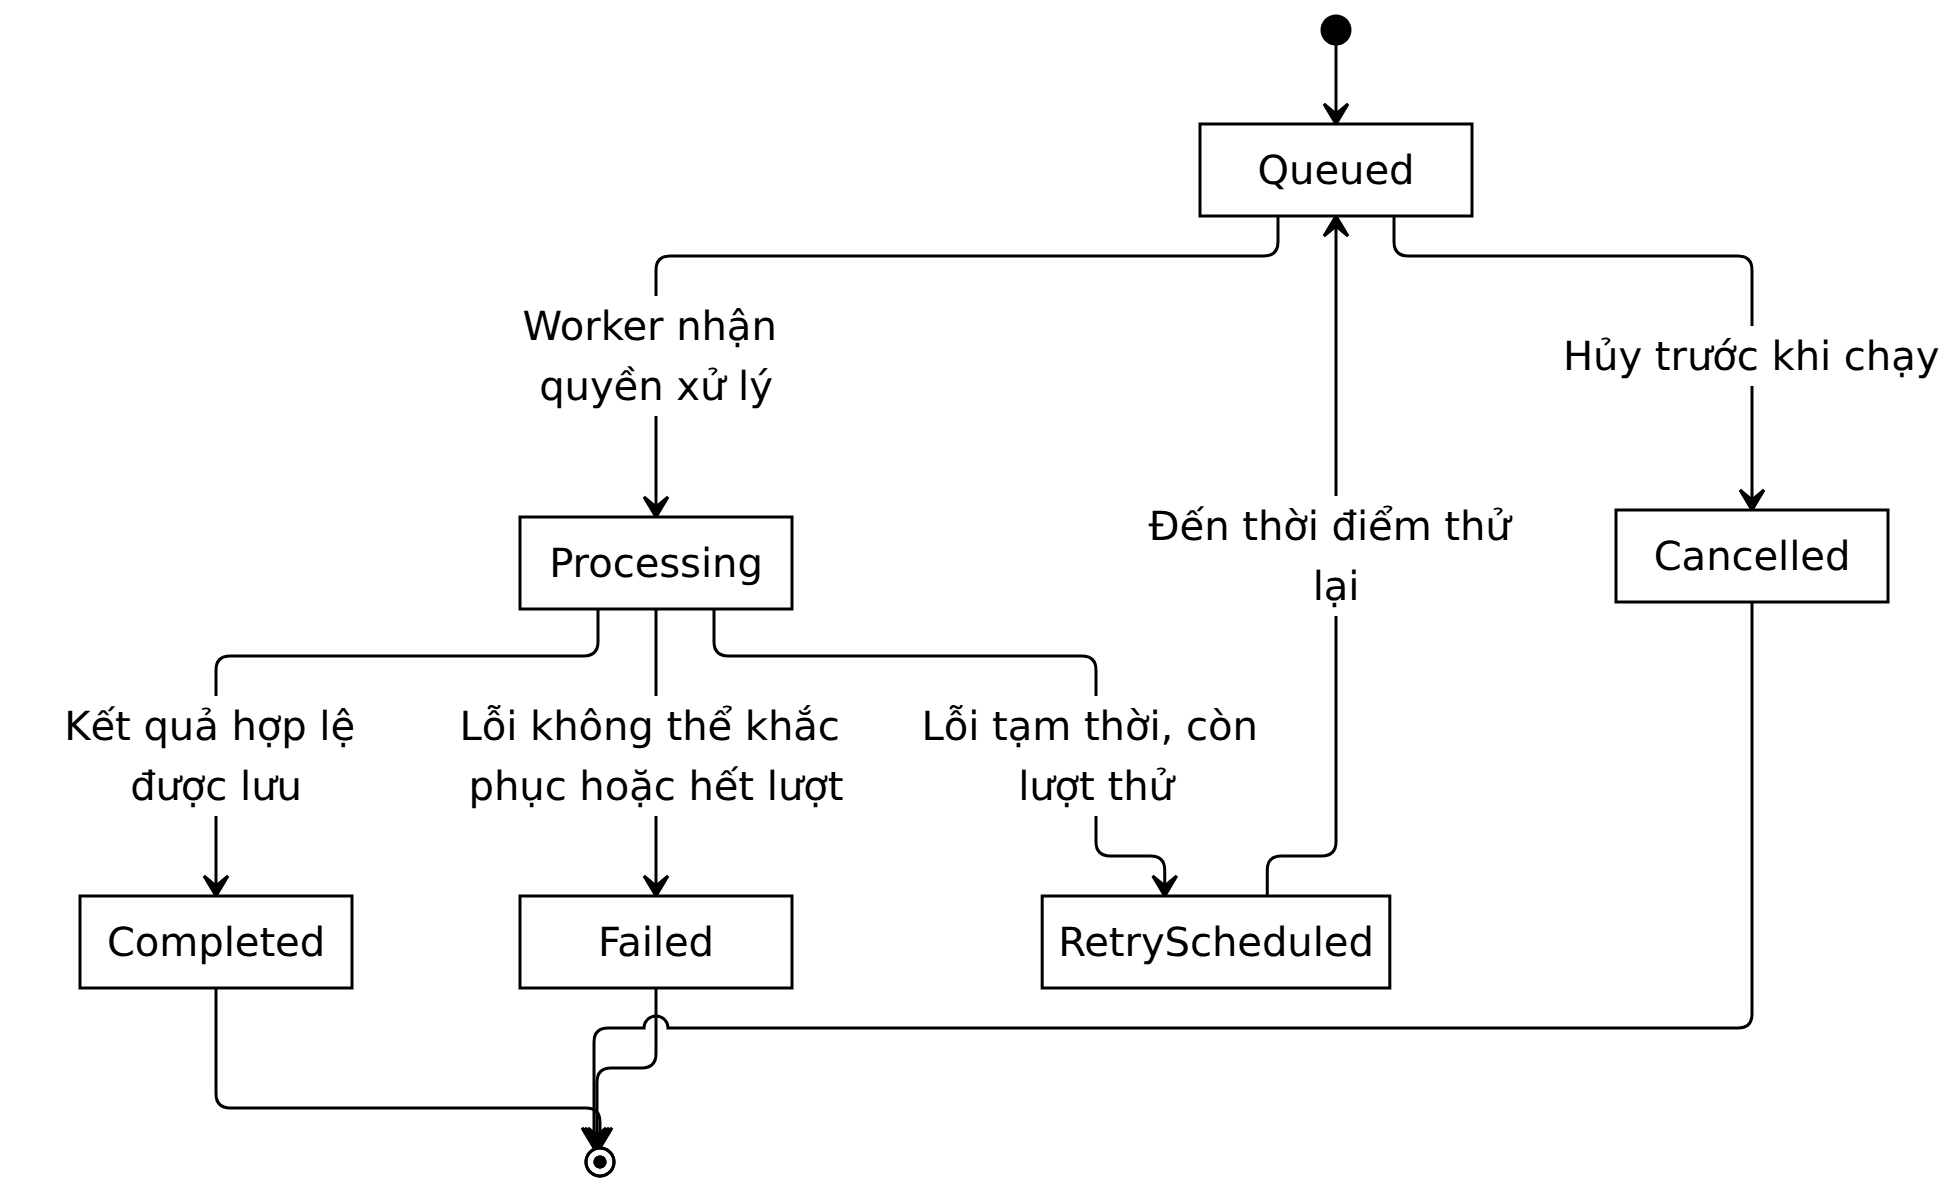
\includegraphics[width=\linewidth,height=.72\textheight,keepaspectratio]{Images/Design/assessment_states.png}
\caption{Vòng đời công việc chấm}
\label{design:fig:assessment_states}
\end{figure}

Thiết kế đề xuất quy định rõ \textbf{tối đa ba lần thực thi tự động cho một job}, gồm lần đầu và hai lần thử lại. Lỗi mạng, timeout có thể khôi phục hoặc lỗi dịch vụ tạm thời được thử lại với khoảng chờ tăng dần. Dữ liệu đầu vào không hợp lệ hoặc phiên bản mô hình không hỗ trợ không được tự động thử lại cùng dữ liệu.

Khi thất bại cuối cùng, Assessment phát sự kiện kết thúc; Core giải phóng phần quota đang giữ hoặc hoàn khoản đã trừ theo loại nghiệp vụ. Việc hoàn được ghi một lần theo mã nghiệp vụ tại Core, không nằm trong transaction lưu kết quả của Assessment. Chấm lại bài thất bại tạo yêu cầu có liên kết tới job trước và áp dụng chính sách miễn trừ quota đã đặc tả; một lần thử kỹ thuật không được biến thành một lượt luyện mới.

Đối với luyện theo Part, quota được giữ khi nhận bài và chốt sau khi chấm thành công. Đối với thi thử, Learning tạo yêu cầu bắt đầu có định danh, Core trừ một lượt thi rồi Learning xác nhận phiên được bắt đầu. Trạng thái bắt đầu dở dang được đối soát như submission; một lần gọi lại dùng cùng mã không trừ thêm lượt. Công việc chấm từng câu dùng ticket của phiên. Assessment tổng hợp trạng thái kết thúc toàn phiên theo manifest trước khi phát quyết định hoàn; không hoàn toàn bộ lượt thi cho mỗi câu bị lỗi. Kết quả phản hồi muộn từ một job đã thất bại cuối cùng không tự động chuyển thành công sau khi quota đã được hoàn.

\paragraph*{Hợp đồng tích hợp với Scoring Model}

FastAPI cung cấp endpoint nội bộ, chẳng hạn \texttt{POST /\allowbreak{}internal/\allowbreak{}v1/\allowbreak{}speaking/\allowbreak{}assessments}. Đây là hợp đồng đề xuất của thiết kế, không phải endpoint đã được xác nhận trong mã nguồn ứng dụng.

Yêu cầu suy luận có thể được chuẩn hóa như sau:

\begingroup\small
\begin{verbatim}
{
  "inferenceId": "uuid-cua-attempt",
  "jobId": "uuid-cua-cong-viec",
  "traceId": "ma-truy-vet",
  "audio": {
    "readUrl": "url-ky-tam-thoi-duoc-cap-khi-thuc-thi",
    "sha256": "checksum-audio",
    "contentType": "audio/webm"
  },
  "question": {
    "part": 2,
    "text": "Describe a skill you would like to learn.",
    "language": "en"
  },
  "modelVersion": "speaking-model-version",
  "rubricVersion": "ielts-speaking-rubric-version"
}
\end{verbatim}
\endgroup

Phản hồi cần chứa \texttt{inference\allowbreak{}Id}, phiên bản mô hình thực tế, phiên bản hợp đồng, transcript có mốc thời gian, điểm FC/LR/GRA/P, band tổng, lỗi và nhận xét. Kết quả phải phân biệt được trường hợp đầy đủ, trường hợp thiếu dữ liệu và trường hợp không đủ điều kiện chấm.

Backend kiểm tra kiểu dữ liệu, miền điểm, mốc thời gian, mã định danh và phiên bản trước khi lưu. Điểm theo thang 0–9, bước 0,5 được xử lý theo hợp đồng đã thống nhất với mô hình. Dữ liệu thiếu tiêu chí bắt buộc không được chuyển thành báo cáo đủ bốn tiêu chí bằng cách điền điểm mặc định.

Scoring Model là thành phần chịu trách nhiệm đánh giá bài nói theo giả định của đề tài. LLM bên ngoài có thể hỗ trợ câu trả lời mẫu hoặc giải thích, nhưng không được tự động thay thế kết quả phát âm và band Speaking của mô hình bằng đánh giá chỉ dựa trên transcript.

\paragraph*{Tiền xử lý và vận hành FastAPI}

AI Runtime gồm các bước kiểm tra tệp, giải mã audio, chuẩn hóa sample rate và số kênh, kiểm tra chất lượng, suy luận, hậu xử lý và kiểm định cấu trúc kết quả. Bản audio gốc được giữ theo chính sách lưu trữ; dữ liệu chuẩn hóa phục vụ suy luận có vòng đời riêng.

Tác vụ GPU nặng không được đặt vào cơ chế \texttt{Background\allowbreak{}Tasks} trong tiến trình HTTP với kỳ vọng có hàng đợi bền vững. FastAPI cũng khuyến nghị sử dụng cơ chế xử lý riêng cho công việc nặng cần chạy qua nhiều tiến trình hoặc máy chủ \cite{ch7_fastapi_tasks}. Trong thiết kế này, .NET Worker và RabbitMQ chịu trách nhiệm điều phối bền vững; FastAPI cung cấp năng lực suy luận có giới hạn đồng thời.

Mô hình được nạp khi tiến trình AI khởi động. Số tiến trình và số yêu cầu chạy đồng thời phải phù hợp bộ nhớ GPU; không tăng số HTTP worker một cách độc lập với số bản sao trọng số. Các bước tính toán đồng bộ được thực thi trong bộ thực thi phù hợp để không chặn event loop của FastAPI. Nếu GPU hết năng lực nhận thêm việc, AI Runtime trả trạng thái quá tải để Worker điều chỉnh nhịp tiếp nhận.

\paragraph*{Thi thử và báo cáo toàn phiên}

Hệ thống tạo trước hoặc cache audio câu hỏi để giảm độ trễ giữa các câu. Trong lúc học viên nói, frontend gửi các đoạn audio theo thứ tự; backend theo dõi phần đã nhận và phần còn thiếu. Kết thúc phiên, hệ thống chỉ tạo các công việc chấm cần thiết sau khi các audio liên quan được xác minh hoàn tất.

Báo cáo thi thử liên kết kết quả theo câu, Part và phiên bản mô hình. Quy tắc tổng hợp phải thuộc hợp đồng đánh giá đã được kiểm chứng của Scoring Model. Backend không tự lấy trung bình tất cả câu để suy ra band toàn bài nếu hợp đồng mô hình chưa quy định. Bài kết thúc sớm được phân biệt với bài đủ phiên và hiển thị kết quả theo phạm vi dữ liệu thực có.

\subsubsection{Sequence diagram các chức năng Wispace}

Các sơ đồ mô tả trao đổi giữa tác nhân, React và dịch vụ sở hữu nghiệp vụ. API Gateway định tuyến và kiểm soát truy cập biên, được lược khỏi các sơ đồ để ưu tiên tương tác dịch vụ. Core, Learning, Assessment và Reporting kiểm tra quyền ở phía mình; ký hiệu DB gắn với từng dịch vụ không biểu diễn database dùng chung. Mũi tên liền biểu diễn lời gọi, mũi tên đứt biểu diễn phản hồi; các khung alt, opt, loop và par biểu diễn nhánh, bước tùy chọn, lặp và xử lý song song. Thông điệp trong luồng nền được tách khỏi phản hồi HTTP để thể hiện đúng thời điểm nhận bài và trả kết quả.

\clearpage
\paragraph*{UC01. Đăng ký tài khoản}

\begin{figure}[H]
\centering
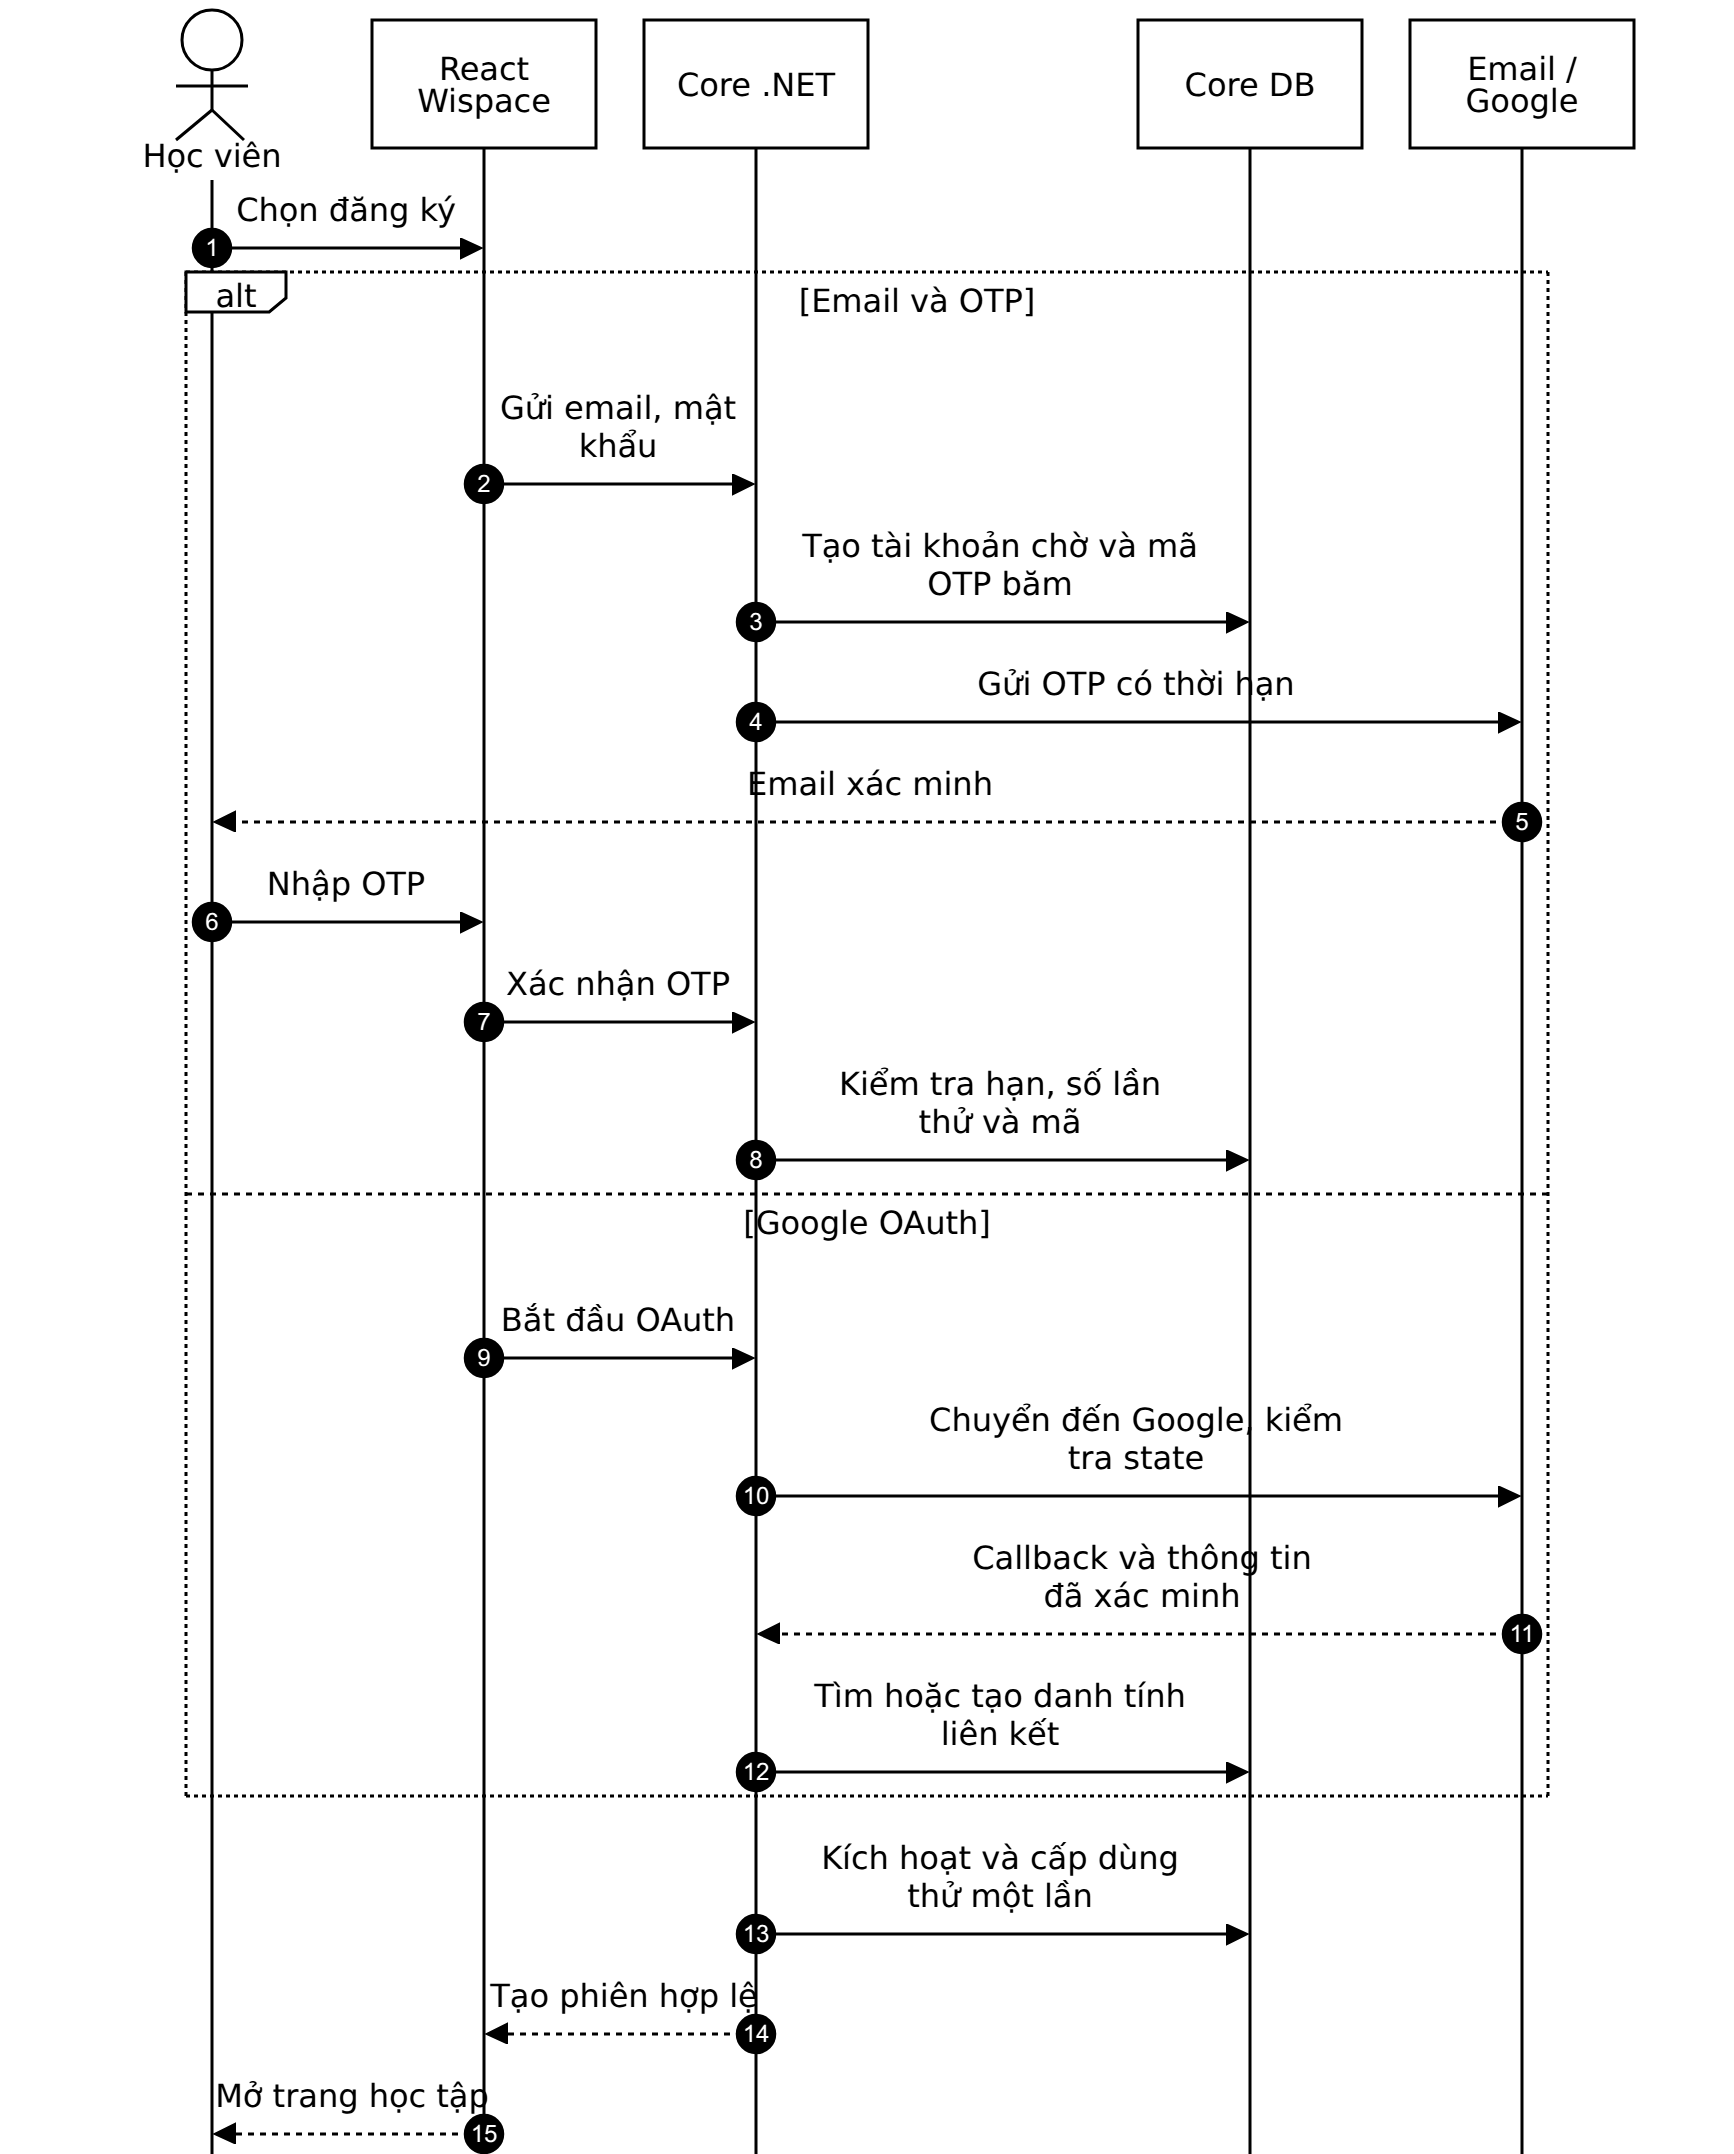
\includegraphics[width=\linewidth,height=.77\textheight,keepaspectratio]{Images/Sequence/Wispace/sequence_uc01_register.png}
\caption{Sequence diagram Wispace UC01 — Đăng ký tài khoản}
\label{sequence:wispace:sequence_uc01_register}
\end{figure}

Hai phương thức đăng ký hội tụ ở bước kích hoạt; cấp quyền lợi dùng thử và tạo tài khoản phải chống lặp.

\clearpage
\paragraph*{UC02. Đăng nhập và khôi phục mật khẩu}

\begin{figure}[H]
\centering
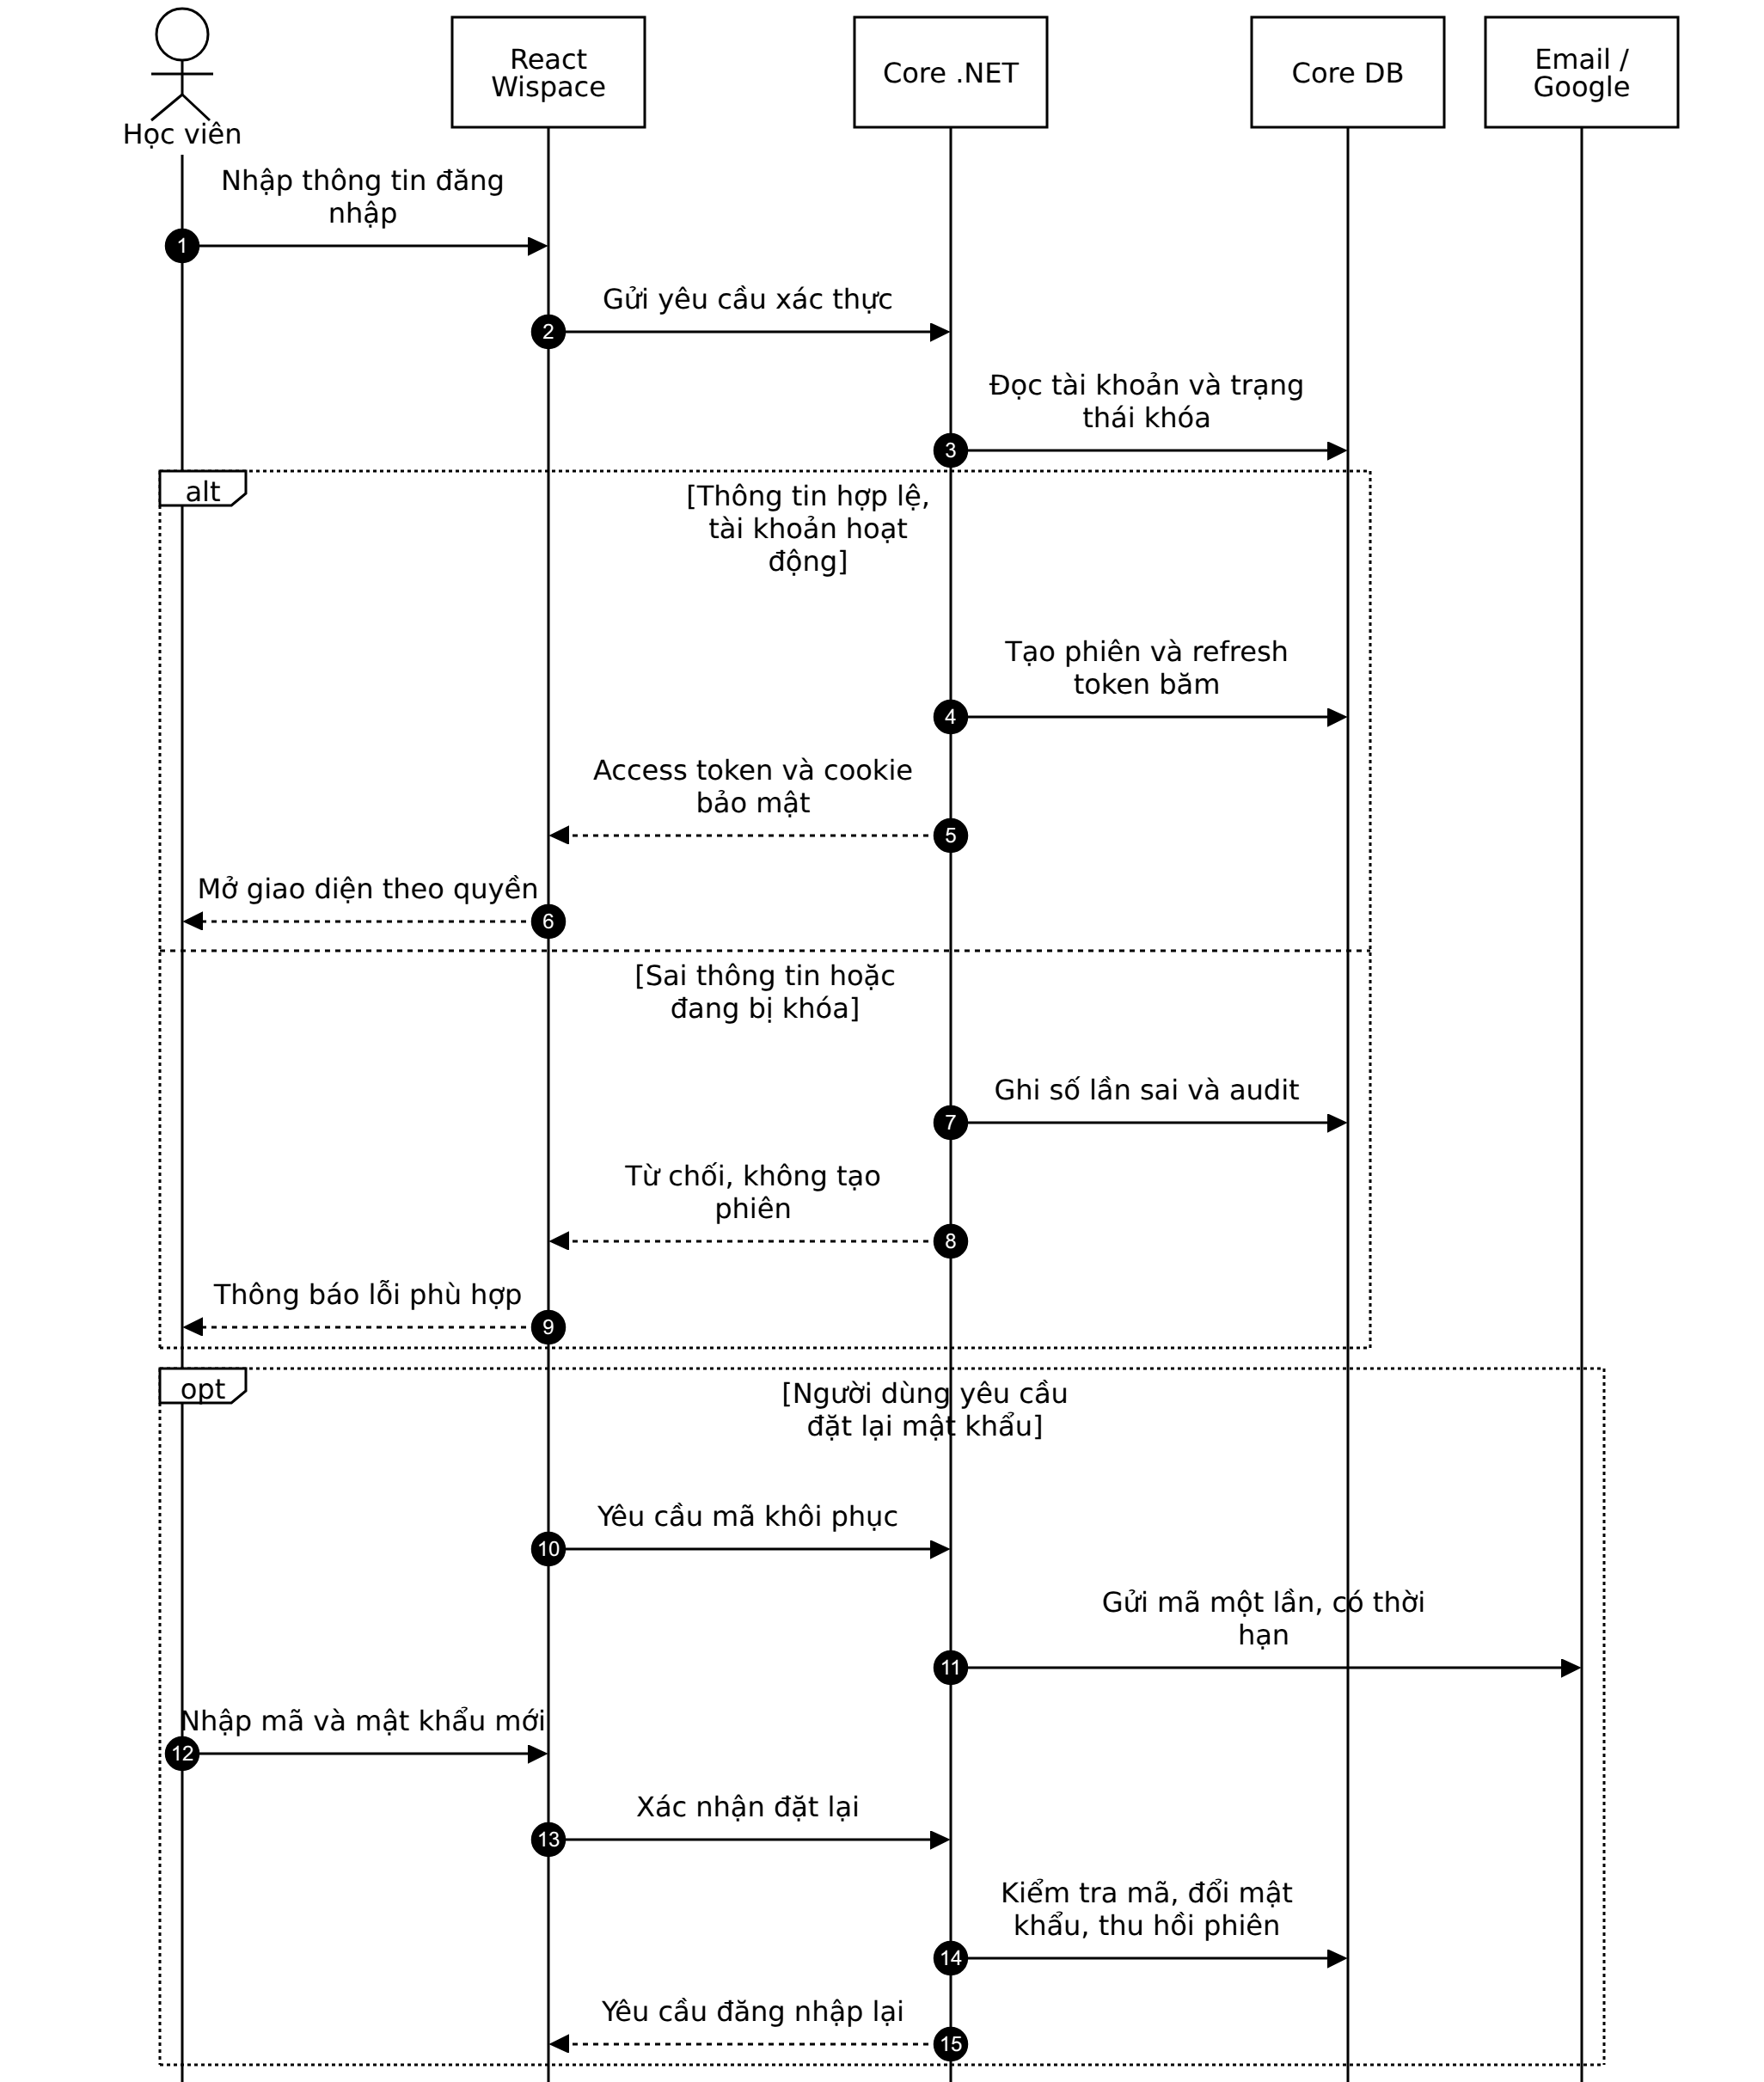
\includegraphics[width=\linewidth,height=.77\textheight,keepaspectratio]{Images/Sequence/Wispace/sequence_uc02_login.png}
\caption{Sequence diagram Wispace UC02 — Đăng nhập và khôi phục mật khẩu}
\label{sequence:wispace:sequence_uc02_login}
\end{figure}

Máy chủ kiểm tra danh tính và trạng thái trước khi cấp phiên; đặt lại mật khẩu thu hồi các phiên cũ.

\clearpage
\paragraph*{UC03. Đăng xuất}

\begin{figure}[H]
\centering
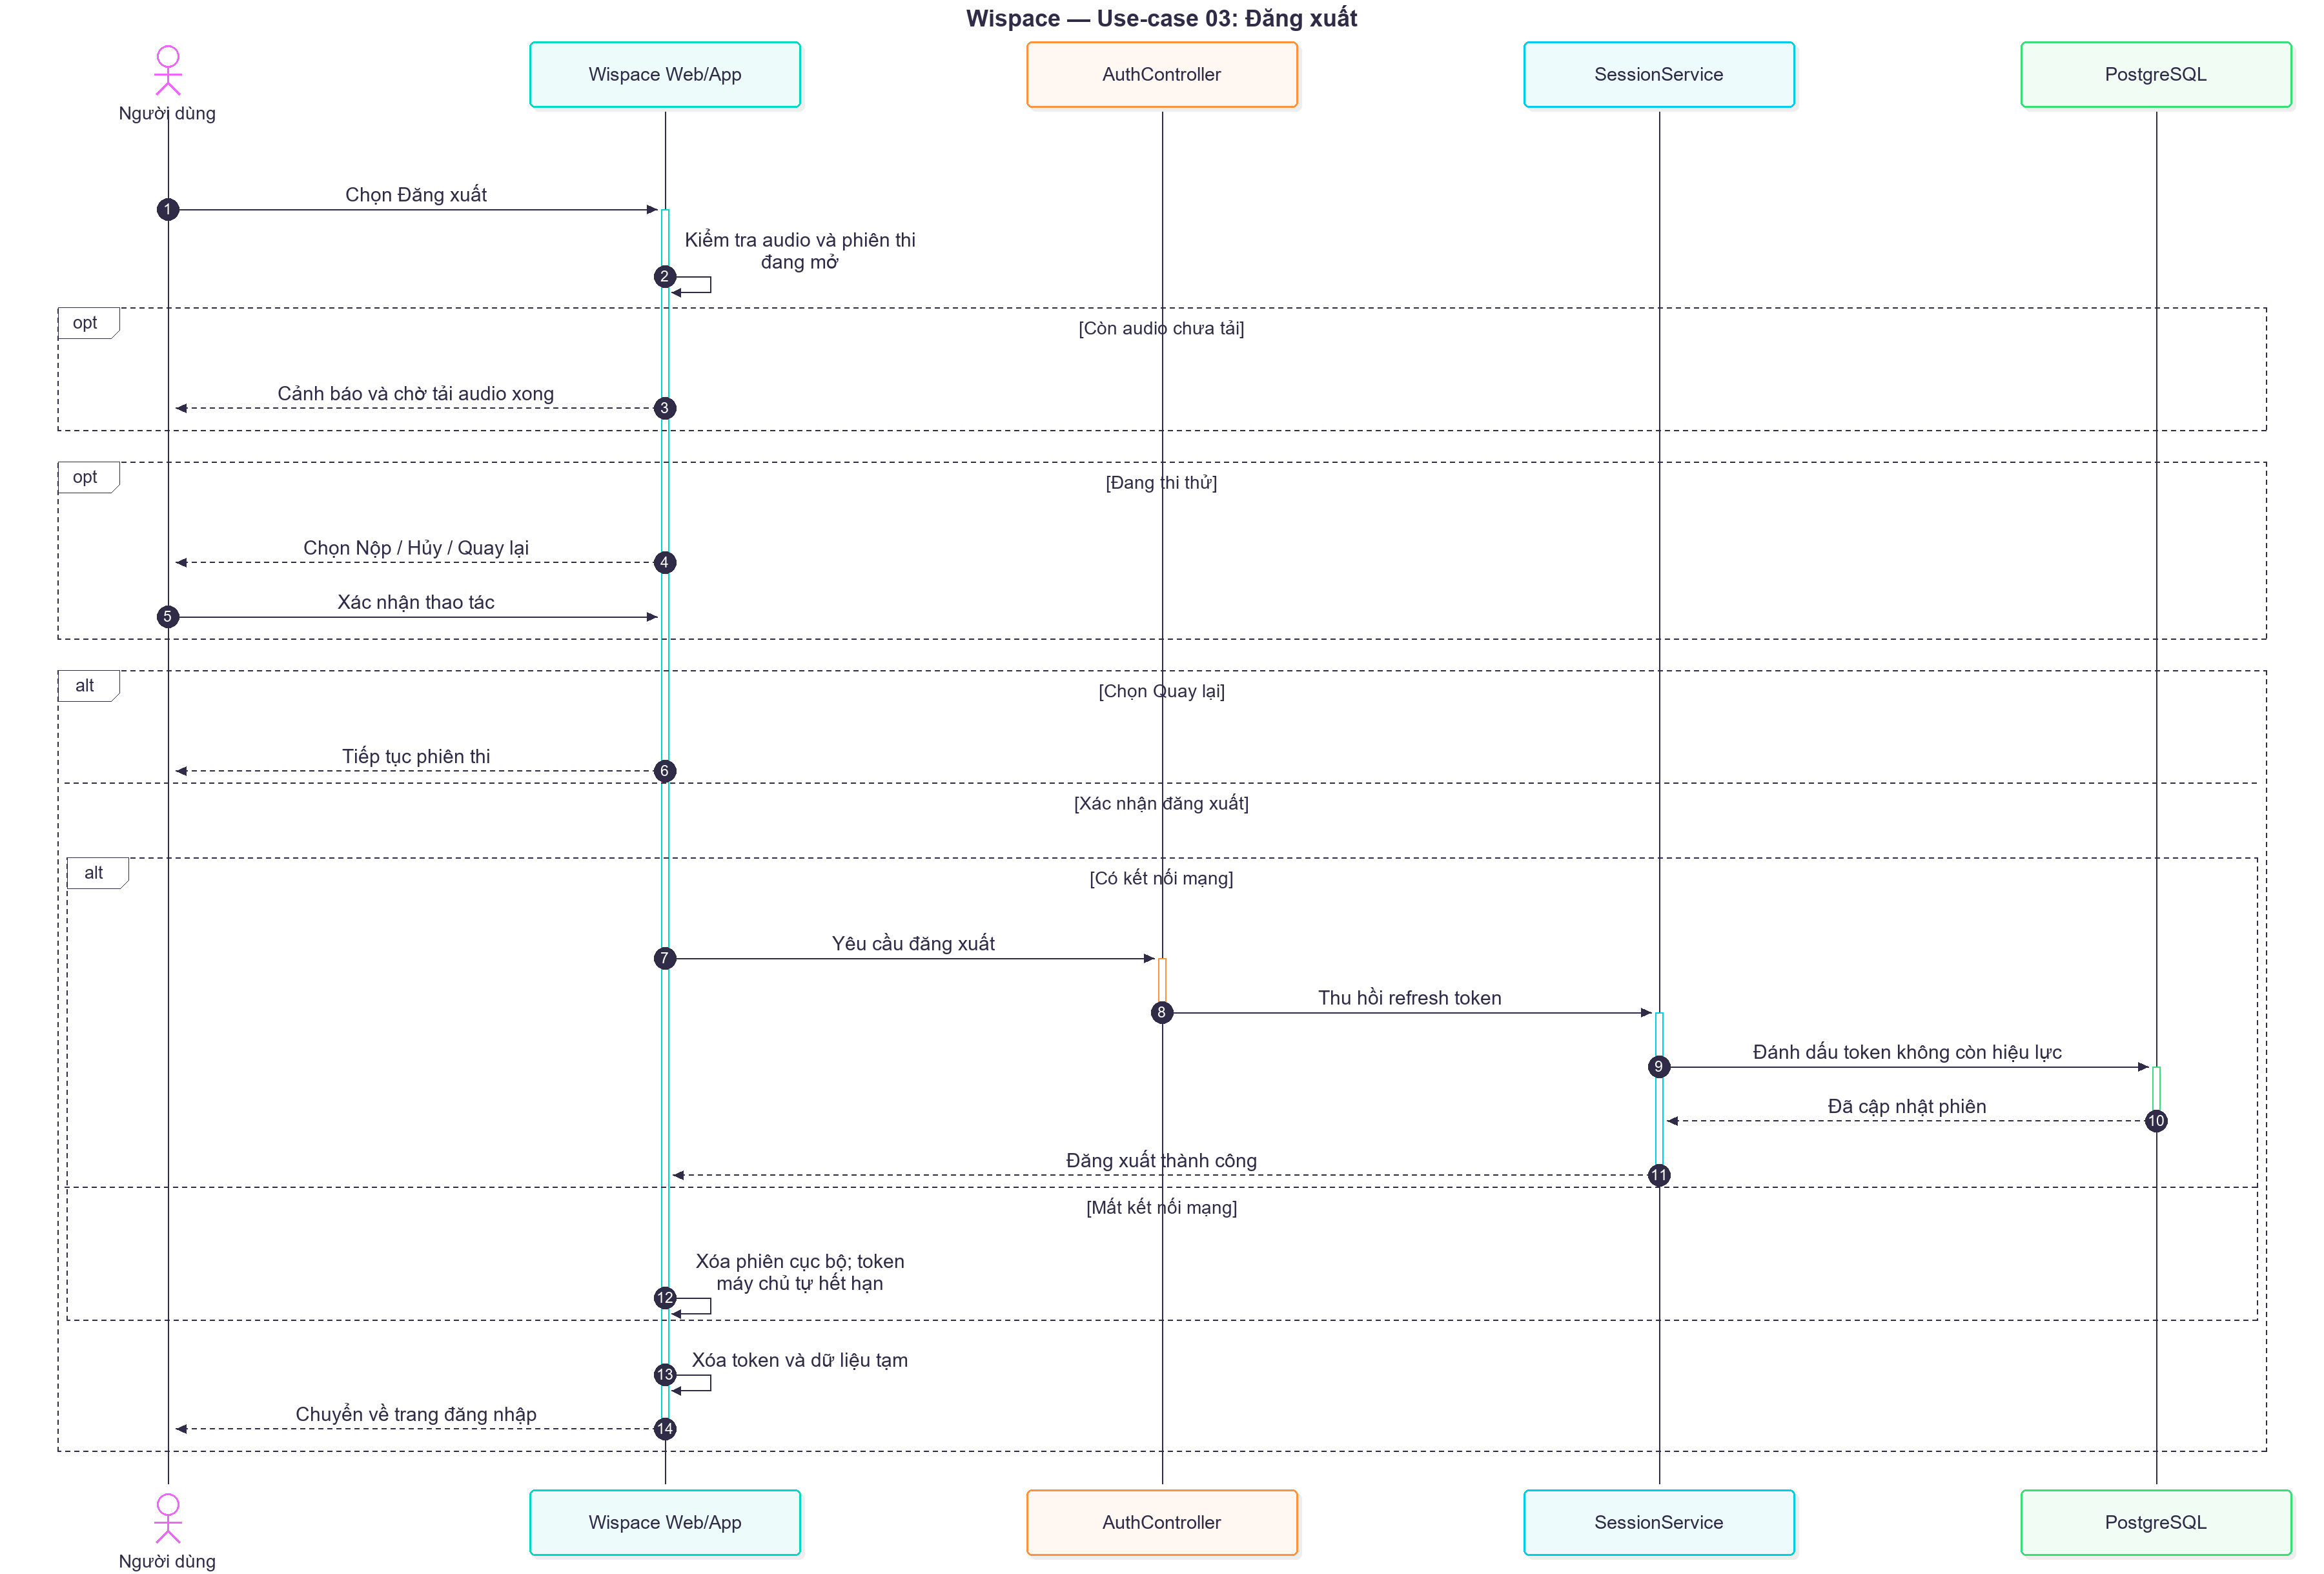
\includegraphics[width=\linewidth,height=.77\textheight,keepaspectratio]{Images/Sequence/Wispace/sequence_uc03_logout.png}
\caption{Sequence diagram Wispace UC03 — Đăng xuất}
\label{sequence:wispace:sequence_uc03_logout}
\end{figure}

Learning lưu bài trong database của mình; Core thu hồi phiên đăng nhập, không ghi trực tiếp dữ liệu phiên thi.

\clearpage
\paragraph*{UC04. Quản lý hồ sơ}

\begin{figure}[H]
\centering
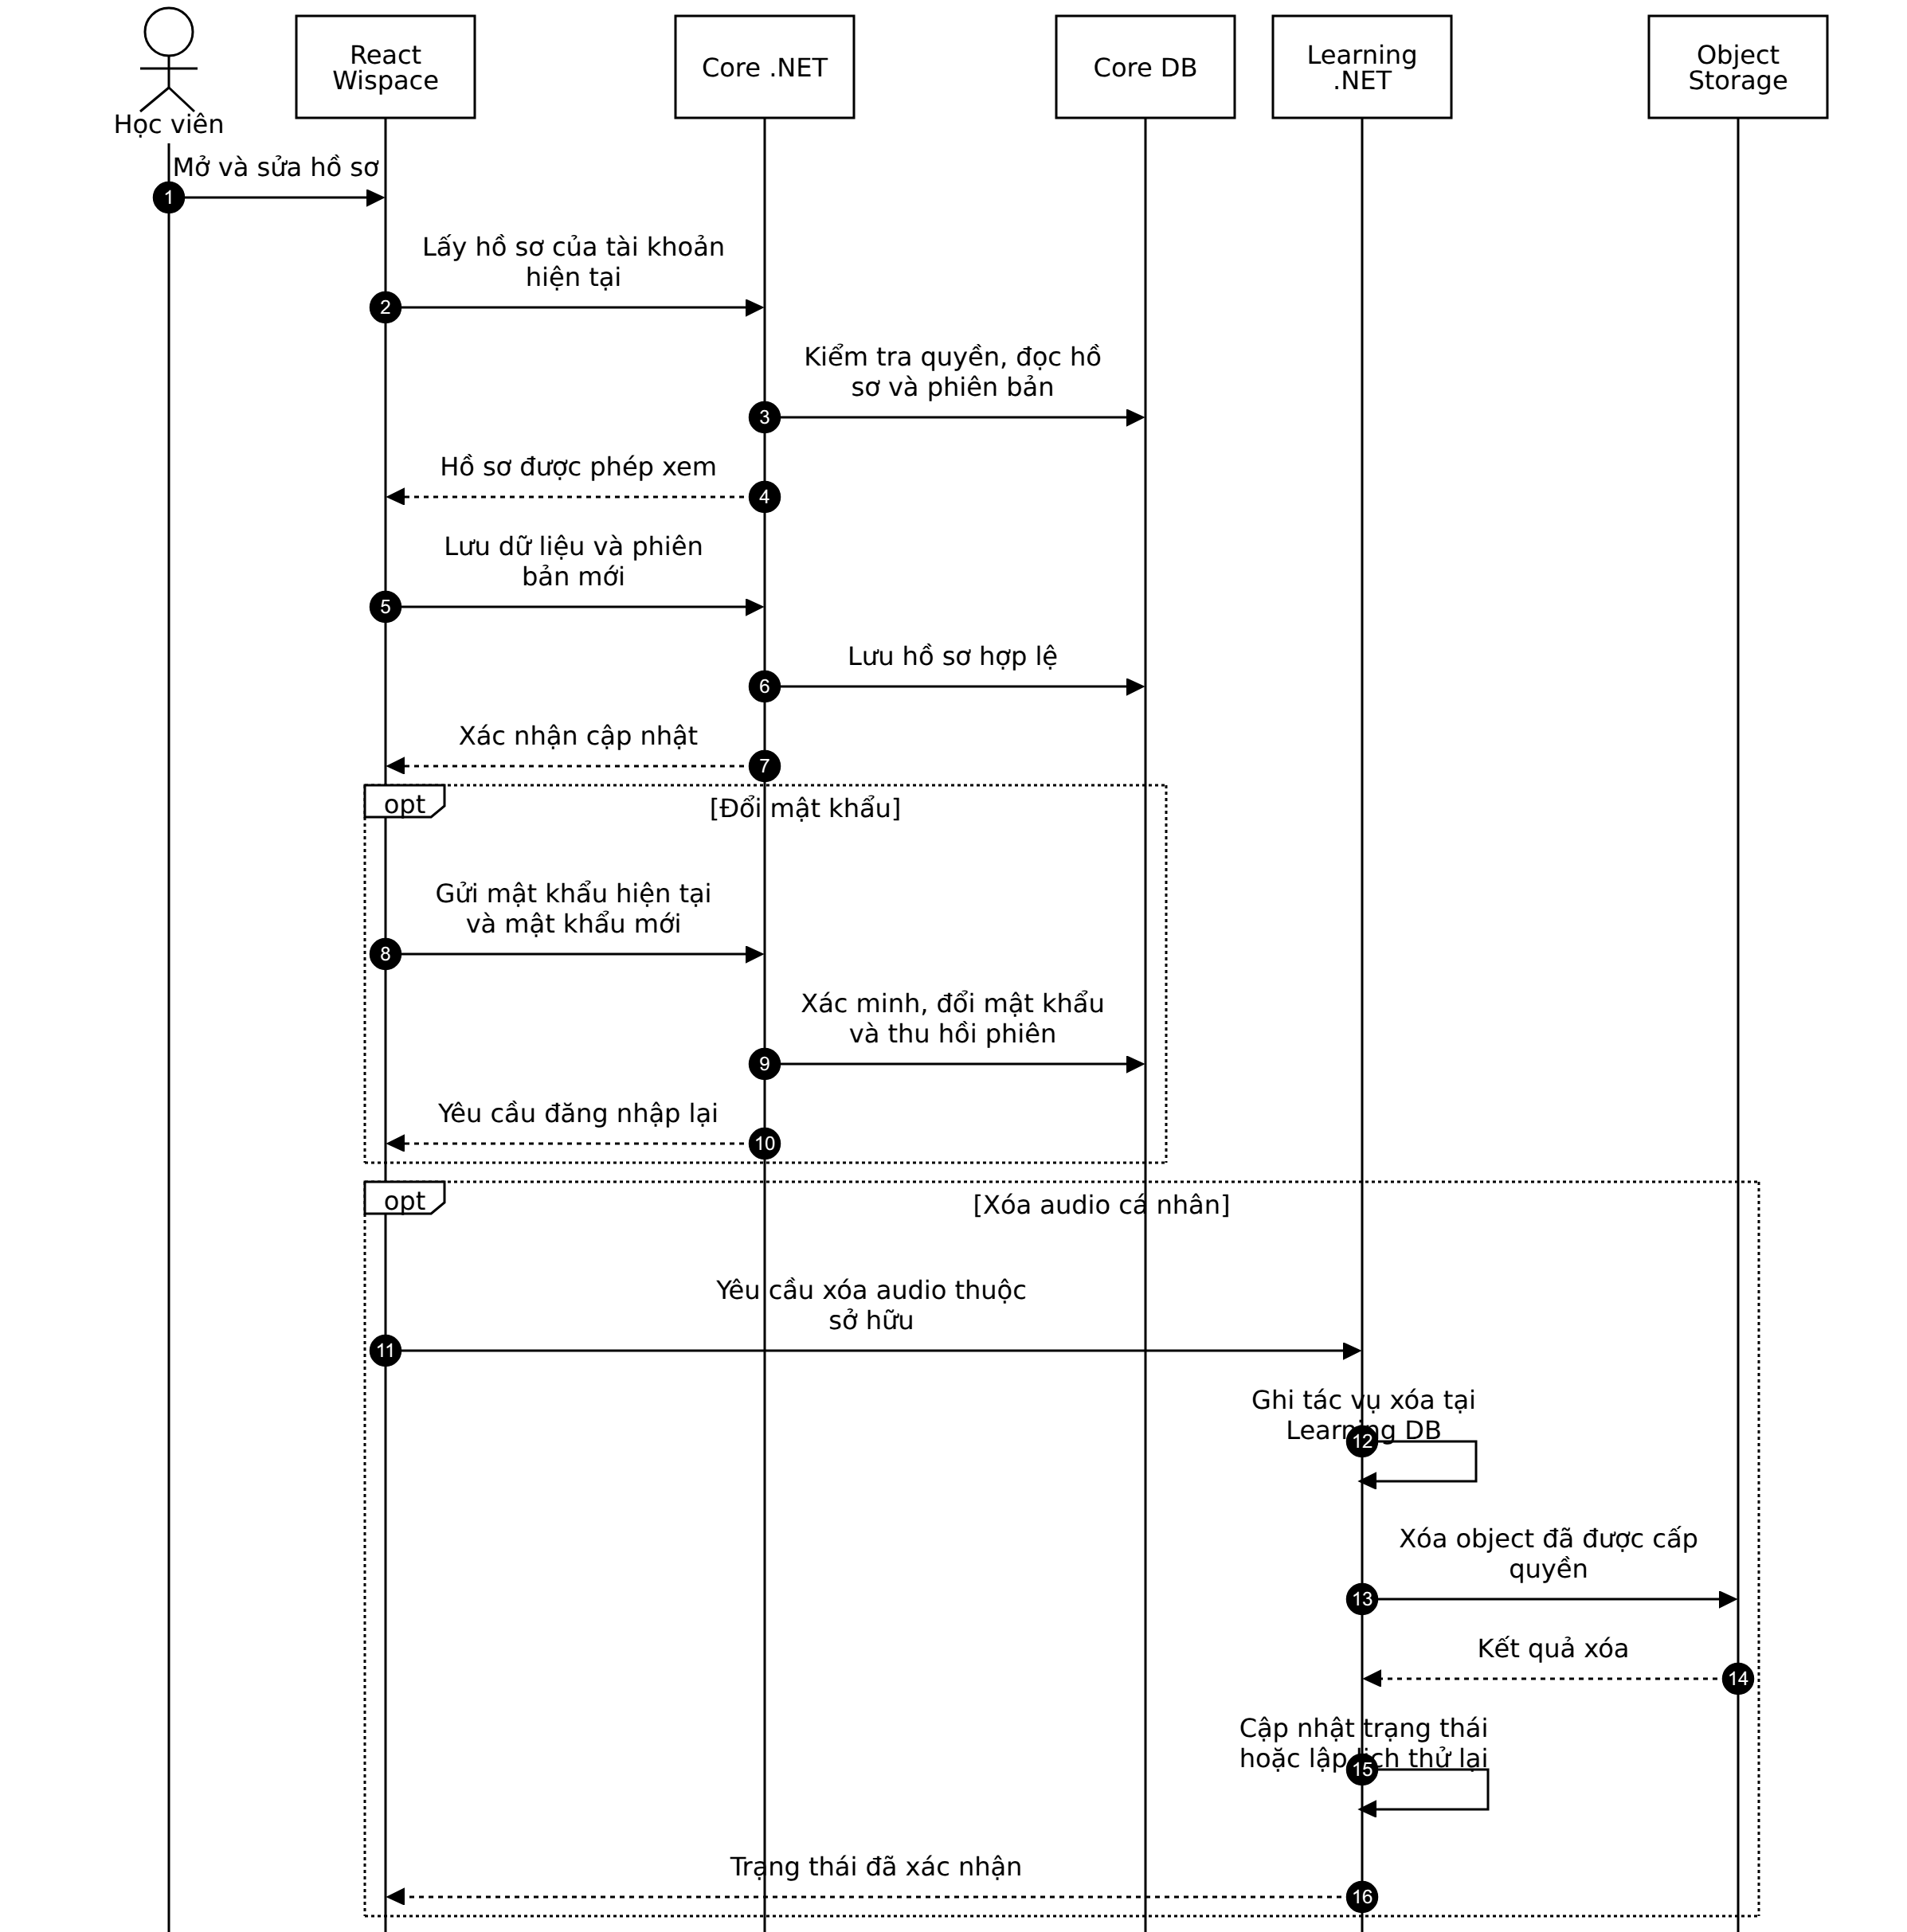
\includegraphics[width=\linewidth,height=.77\textheight,keepaspectratio]{Images/Sequence/Wispace/sequence_uc04_profile.png}
\caption{Sequence diagram Wispace UC04 — Quản lý hồ sơ}
\label{sequence:wispace:sequence_uc04_profile}
\end{figure}

Core quản lý hồ sơ; Learning quản lý quyền audio và trạng thái xóa, không có truy cập chéo database.

\clearpage
\paragraph*{UC05. Quản trị người dùng}

\begin{figure}[H]
\centering
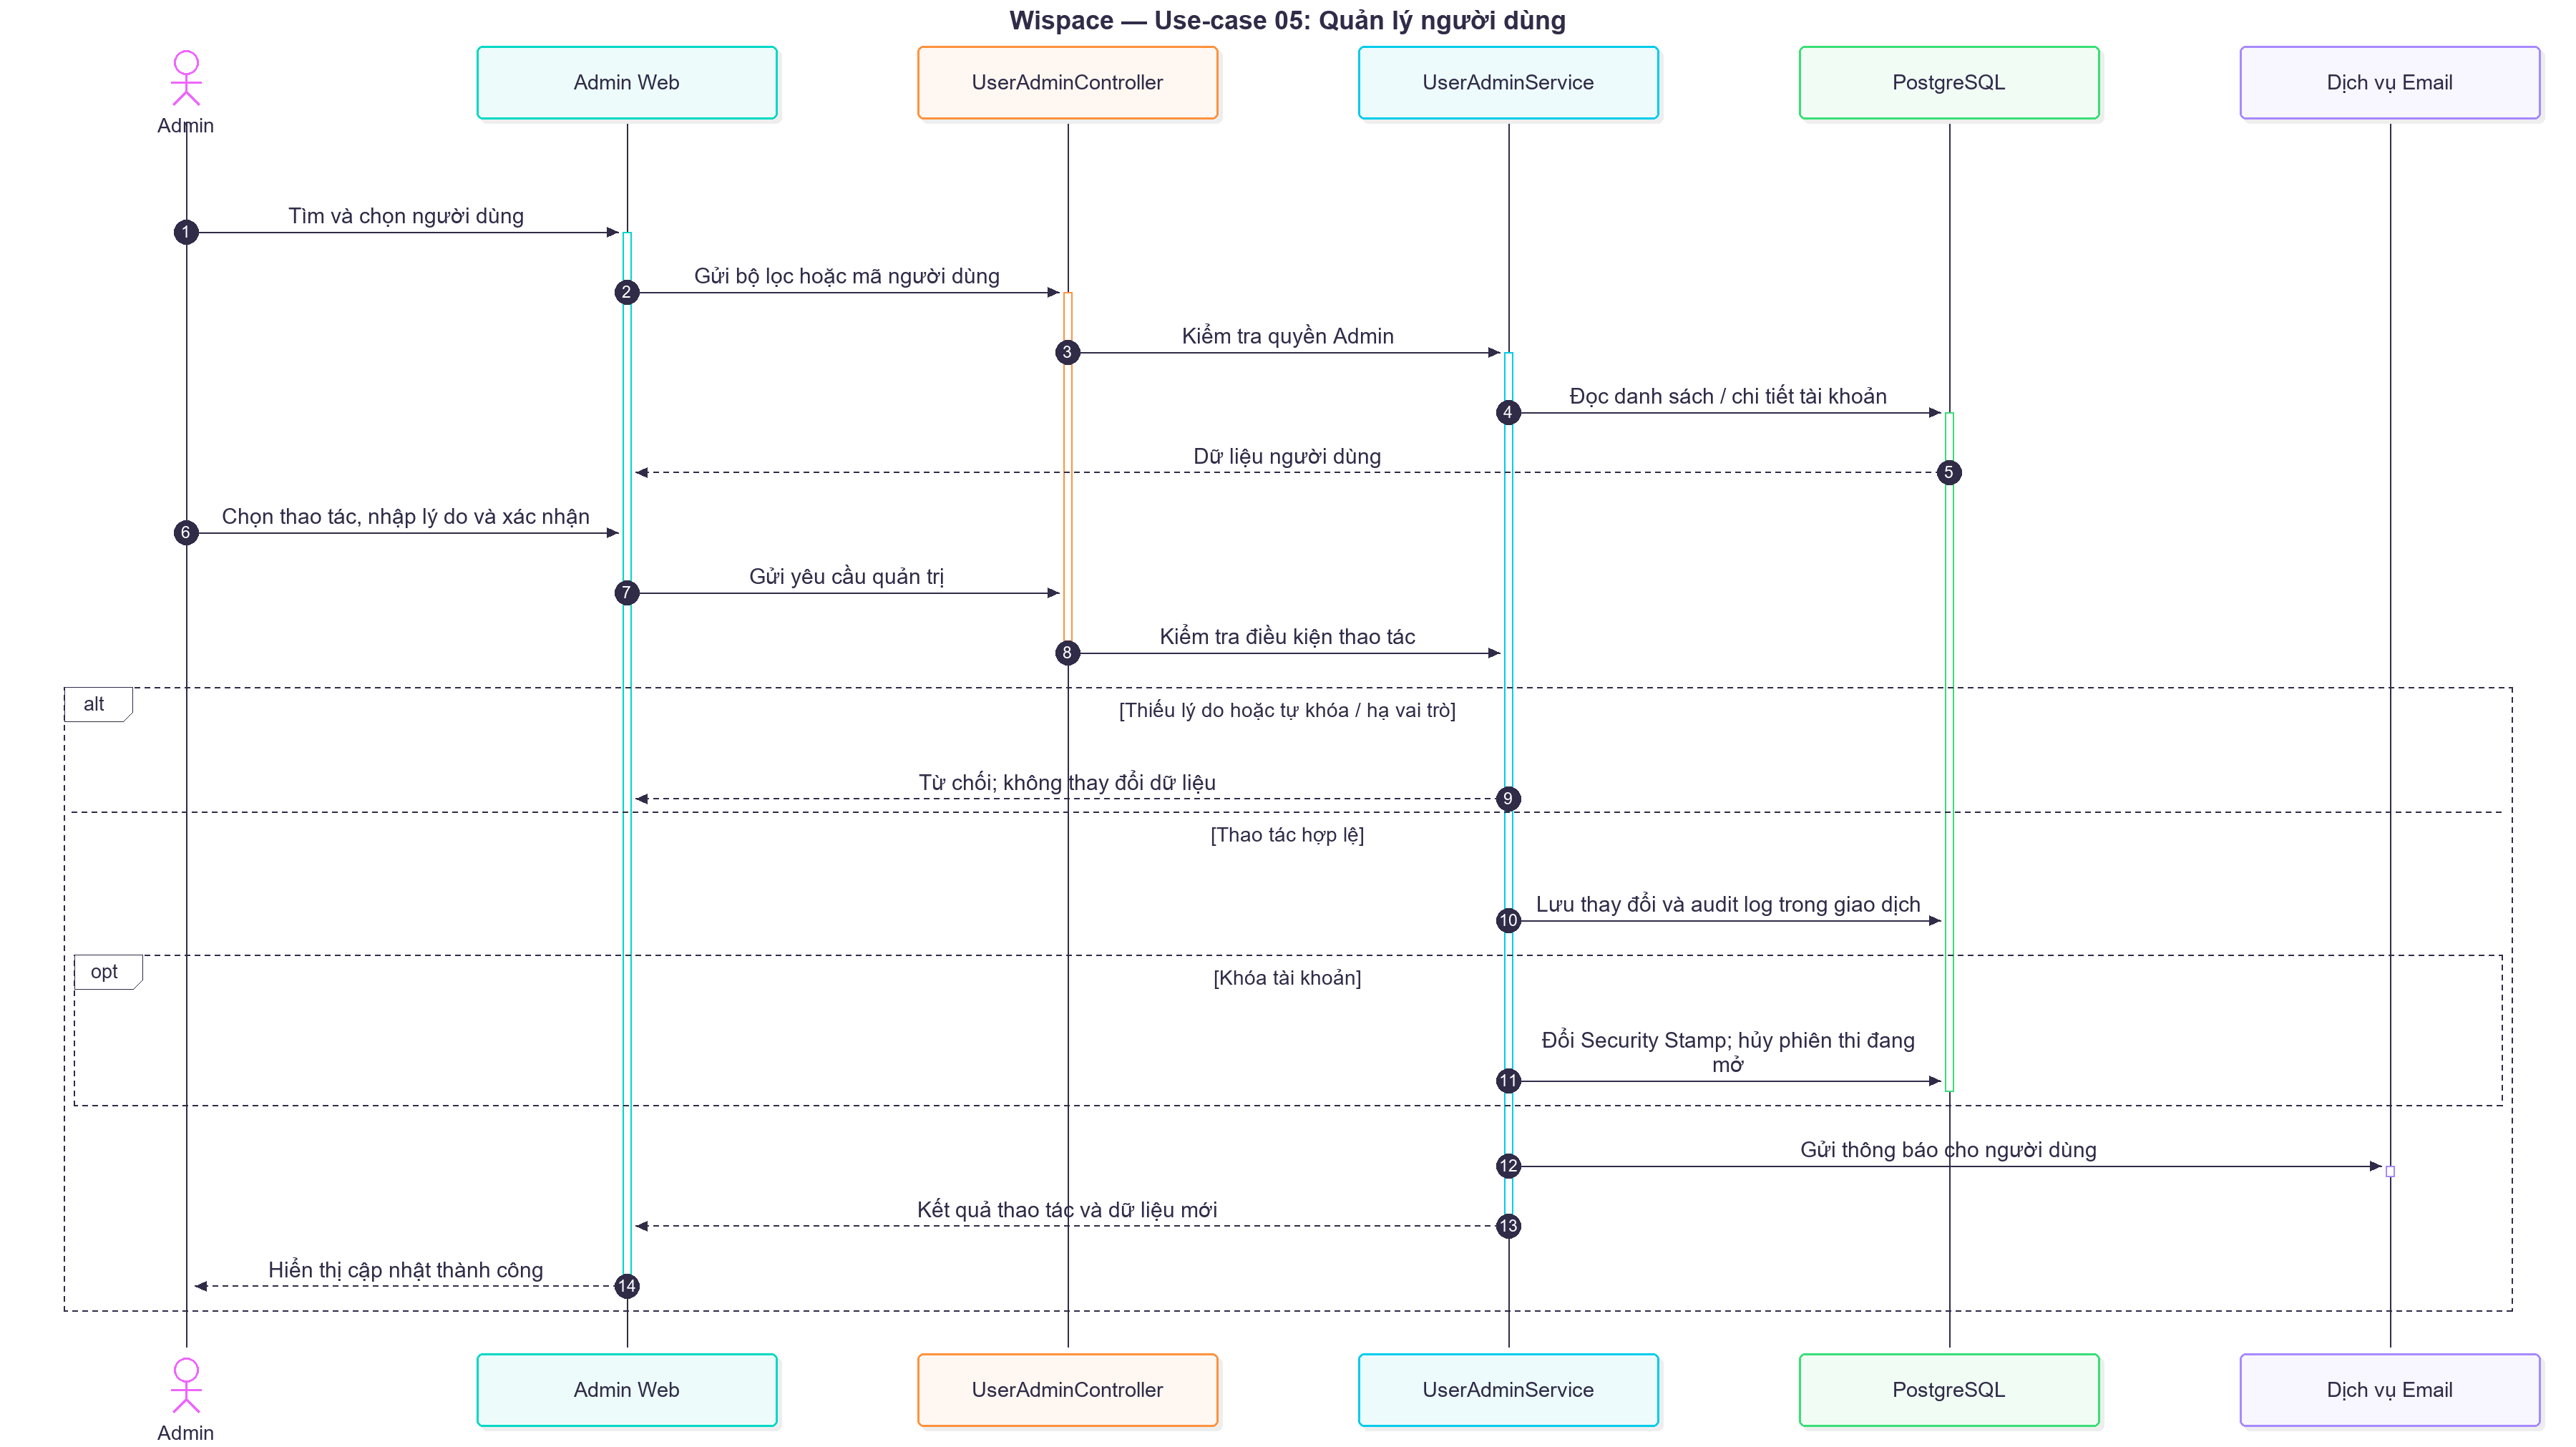
\includegraphics[width=\linewidth,height=.77\textheight,keepaspectratio]{Images/Sequence/Wispace/sequence_uc05_user_management.png}
\caption{Sequence diagram Wispace UC05 — Quản trị người dùng}
\label{sequence:wispace:sequence_uc05_user_management}
\end{figure}

Kiểm tra quyền và quy tắc tài khoản trước giao dịch; thay đổi nhạy cảm gắn với kiểm toán và thu hồi phiên.

\clearpage
\paragraph*{UC06. Xem và tìm kiếm đề}

\begin{figure}[H]
\centering
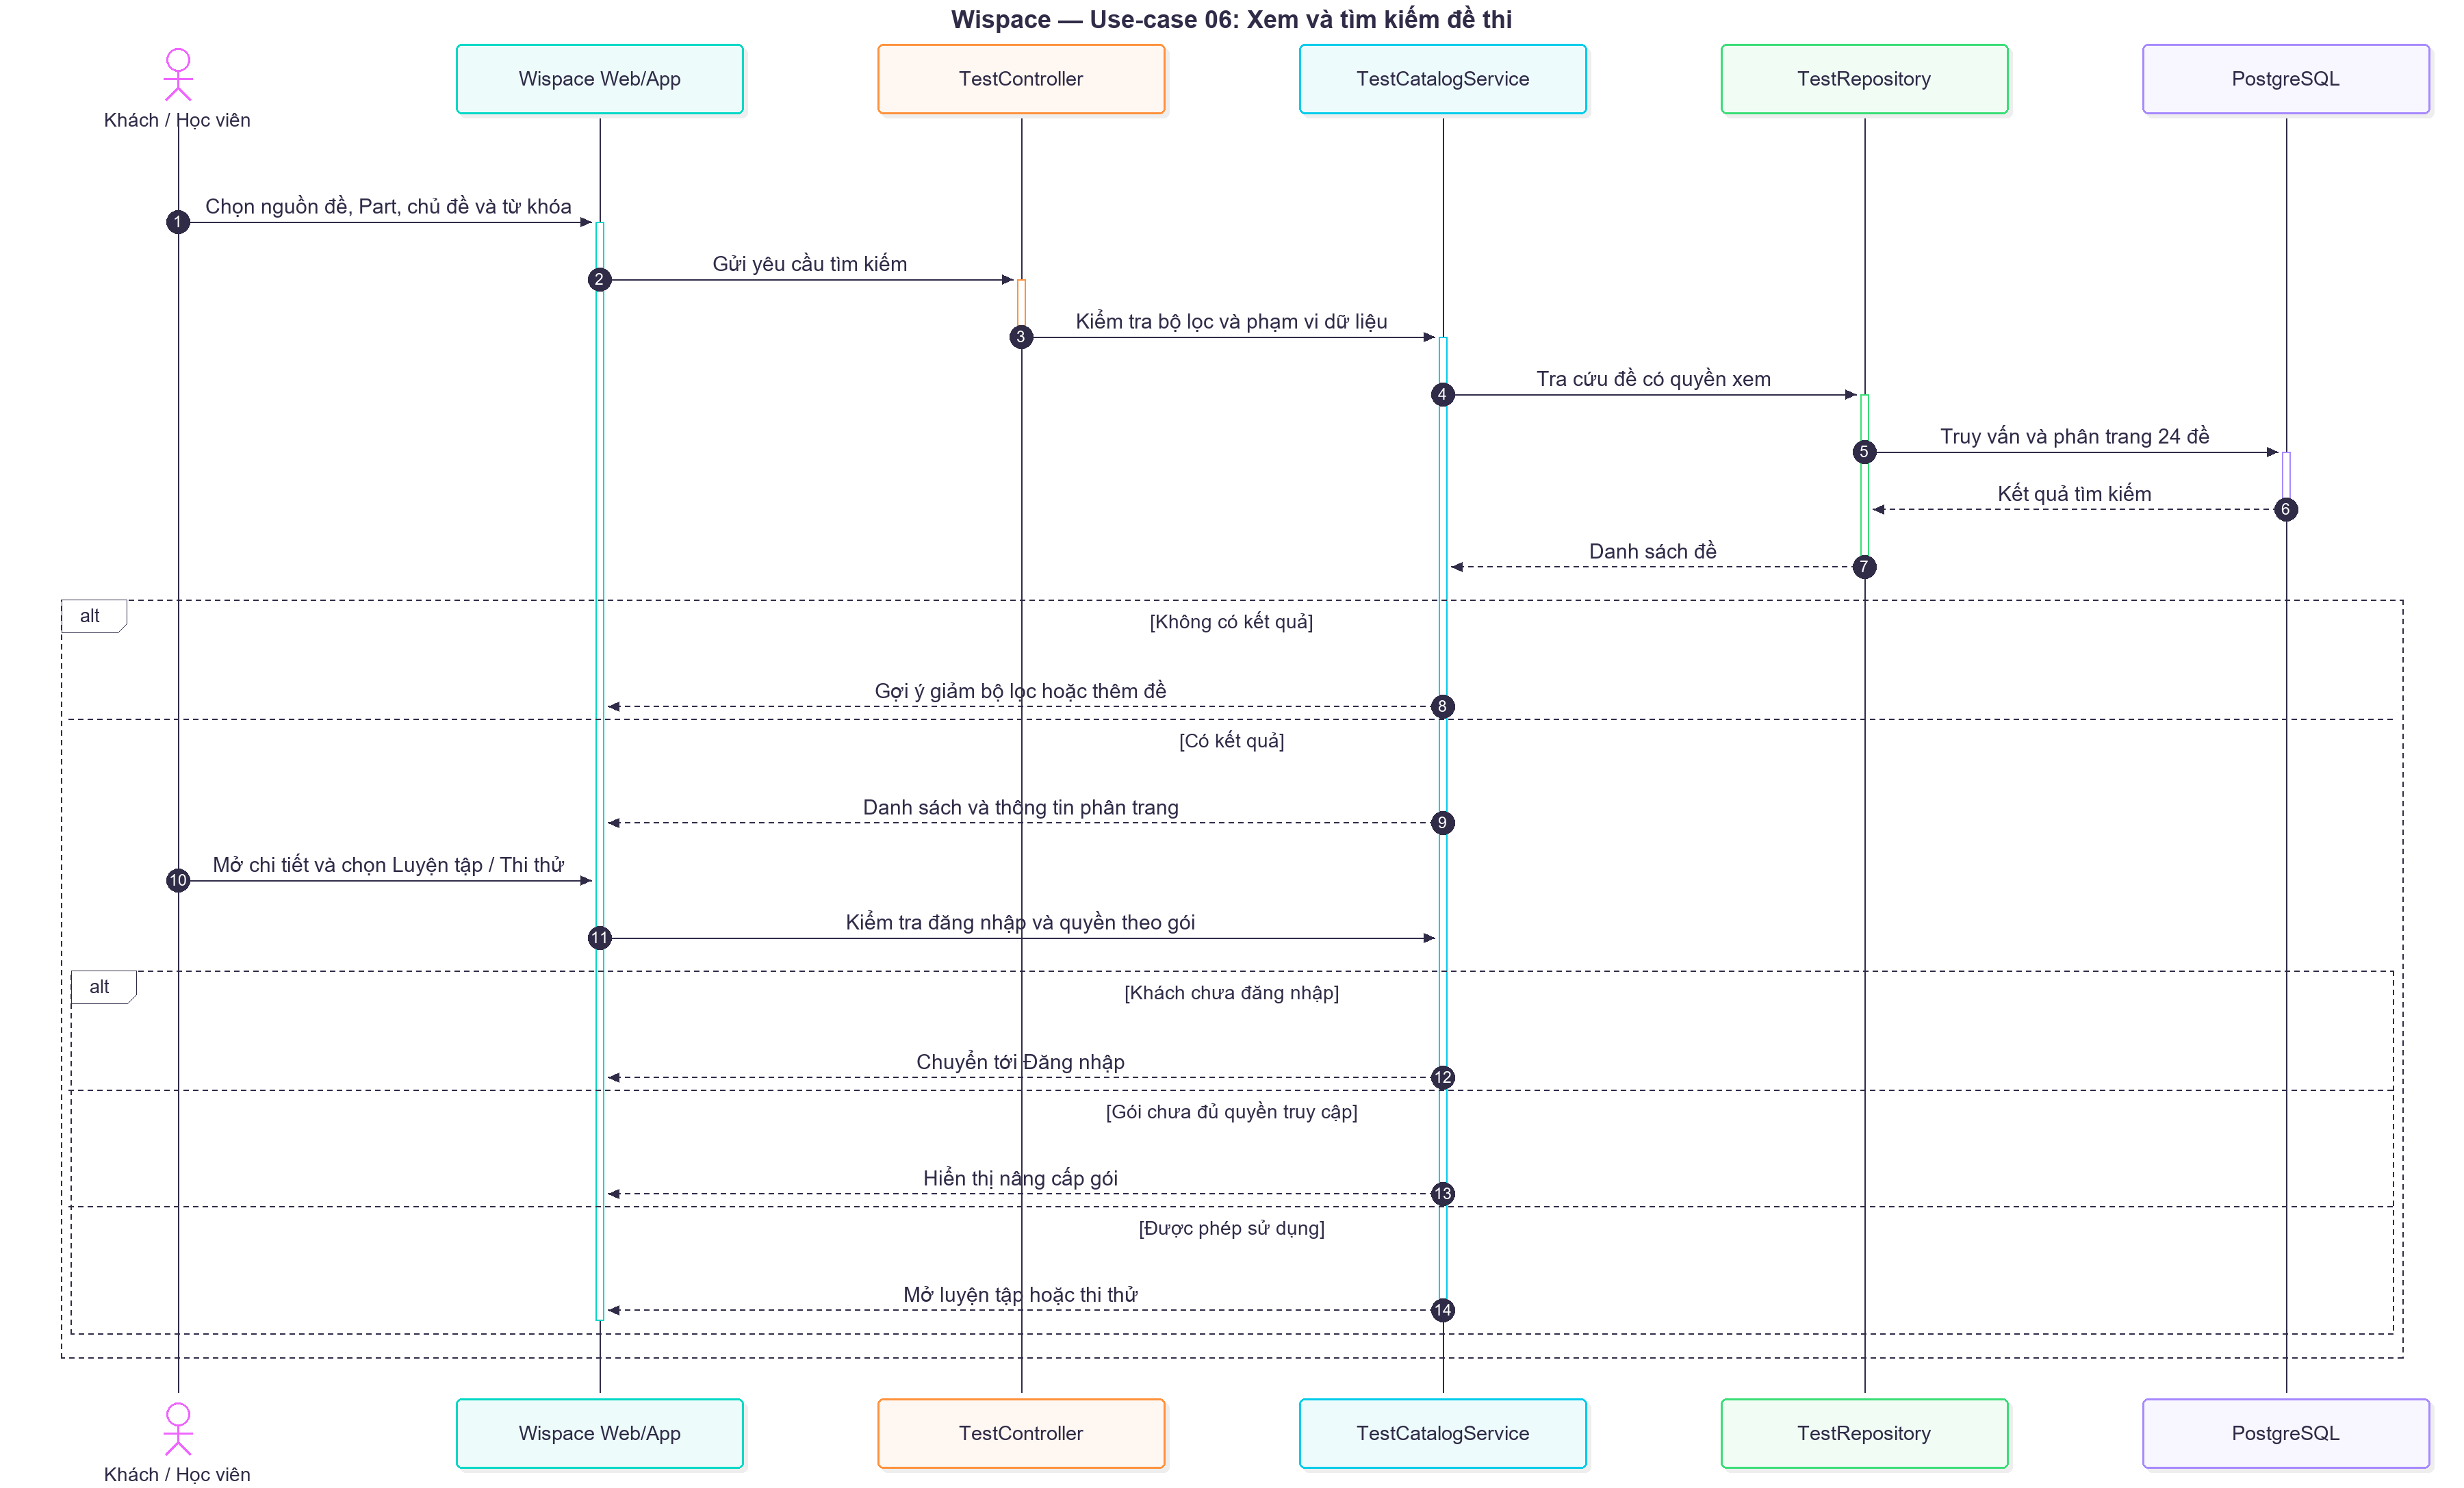
\includegraphics[width=\linewidth,height=.77\textheight,keepaspectratio]{Images/Sequence/Wispace/sequence_uc06_browse_tests.png}
\caption{Sequence diagram Wispace UC06 — Xem và tìm kiếm đề}
\label{sequence:wispace:sequence_uc06_browse_tests}
\end{figure}

Bộ lọc quyền được áp dụng trong truy vấn và kiểm tra lại ở trang chi tiết; quyền xem không đồng nghĩa quyền thi.

\clearpage
\paragraph*{UC07. Thêm đề luyện tập}

\begin{figure}[H]
\centering
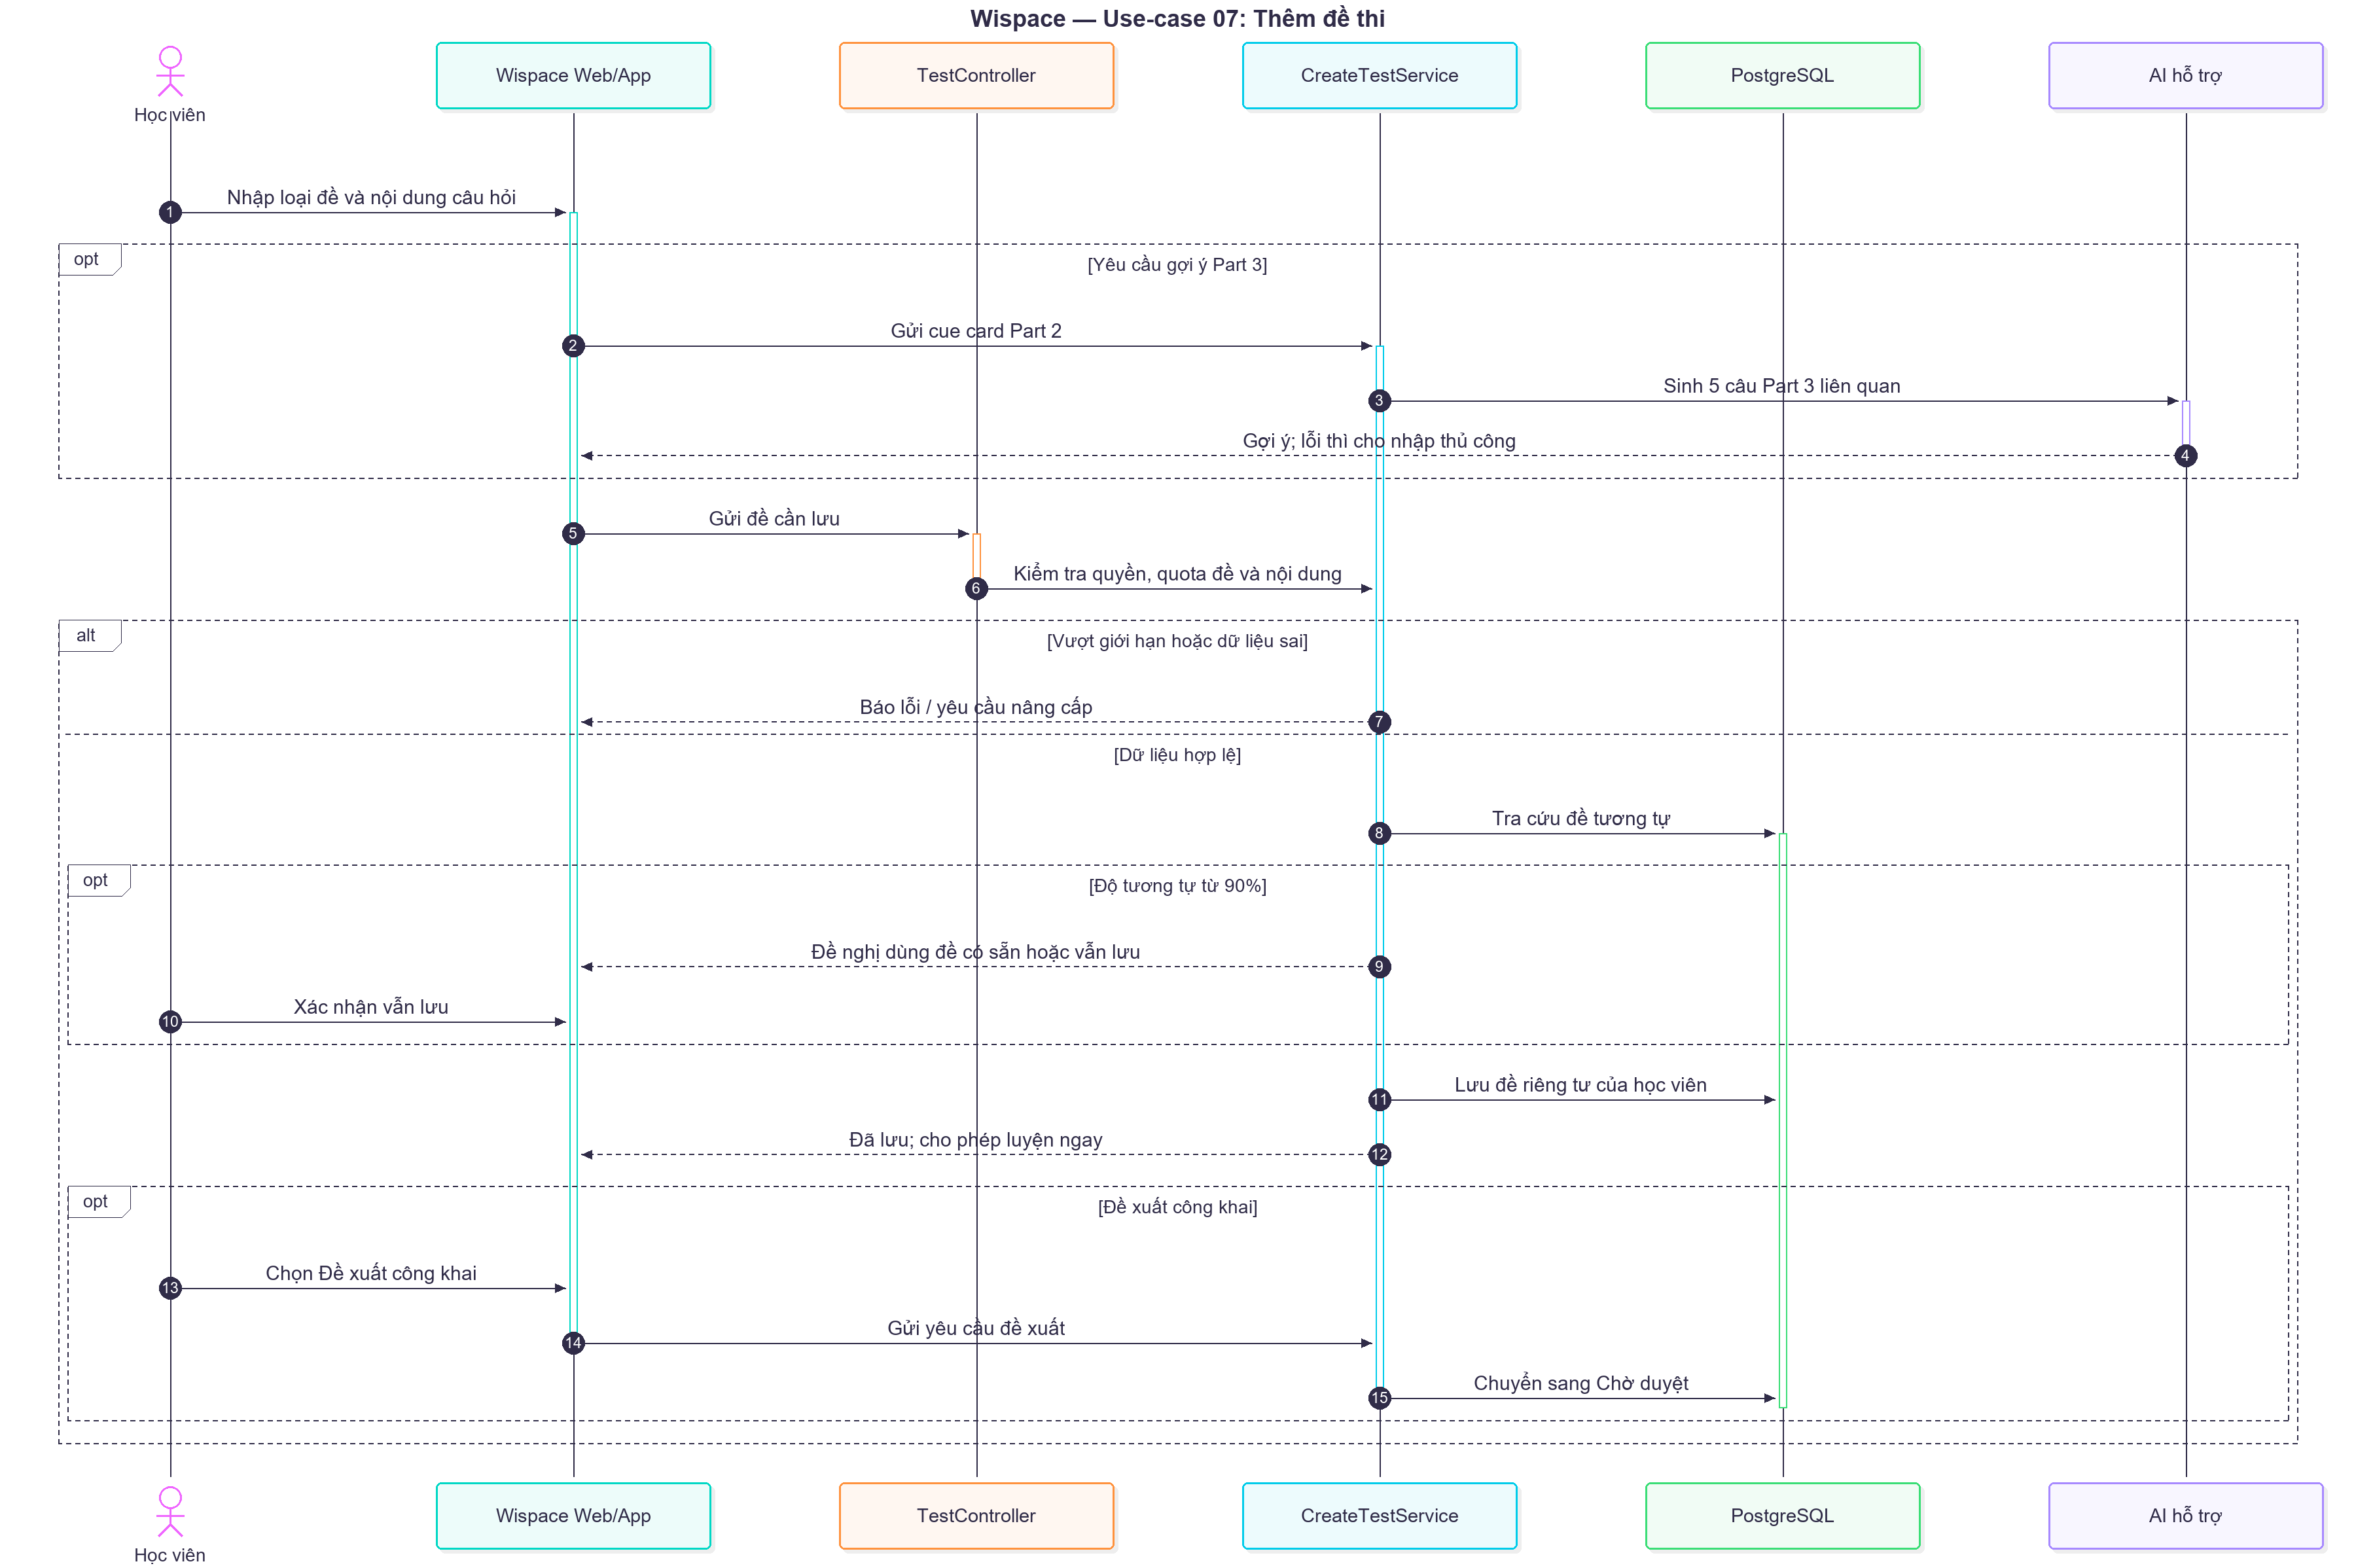
\includegraphics[width=\linewidth,height=.77\textheight,keepaspectratio]{Images/Sequence/Wispace/sequence_uc07_add_test.png}
\caption{Sequence diagram Wispace UC07 — Thêm đề luyện tập}
\label{sequence:wispace:sequence_uc07_add_test}
\end{figure}

Đề được lưu riêng tư sau kiểm tra toàn bộ; lỗi TTS không làm mất đề và đề xuất công khai cần kiểm duyệt.

\clearpage
\paragraph*{UC08. Quản lý và kiểm duyệt đề}

\begin{figure}[H]
\centering
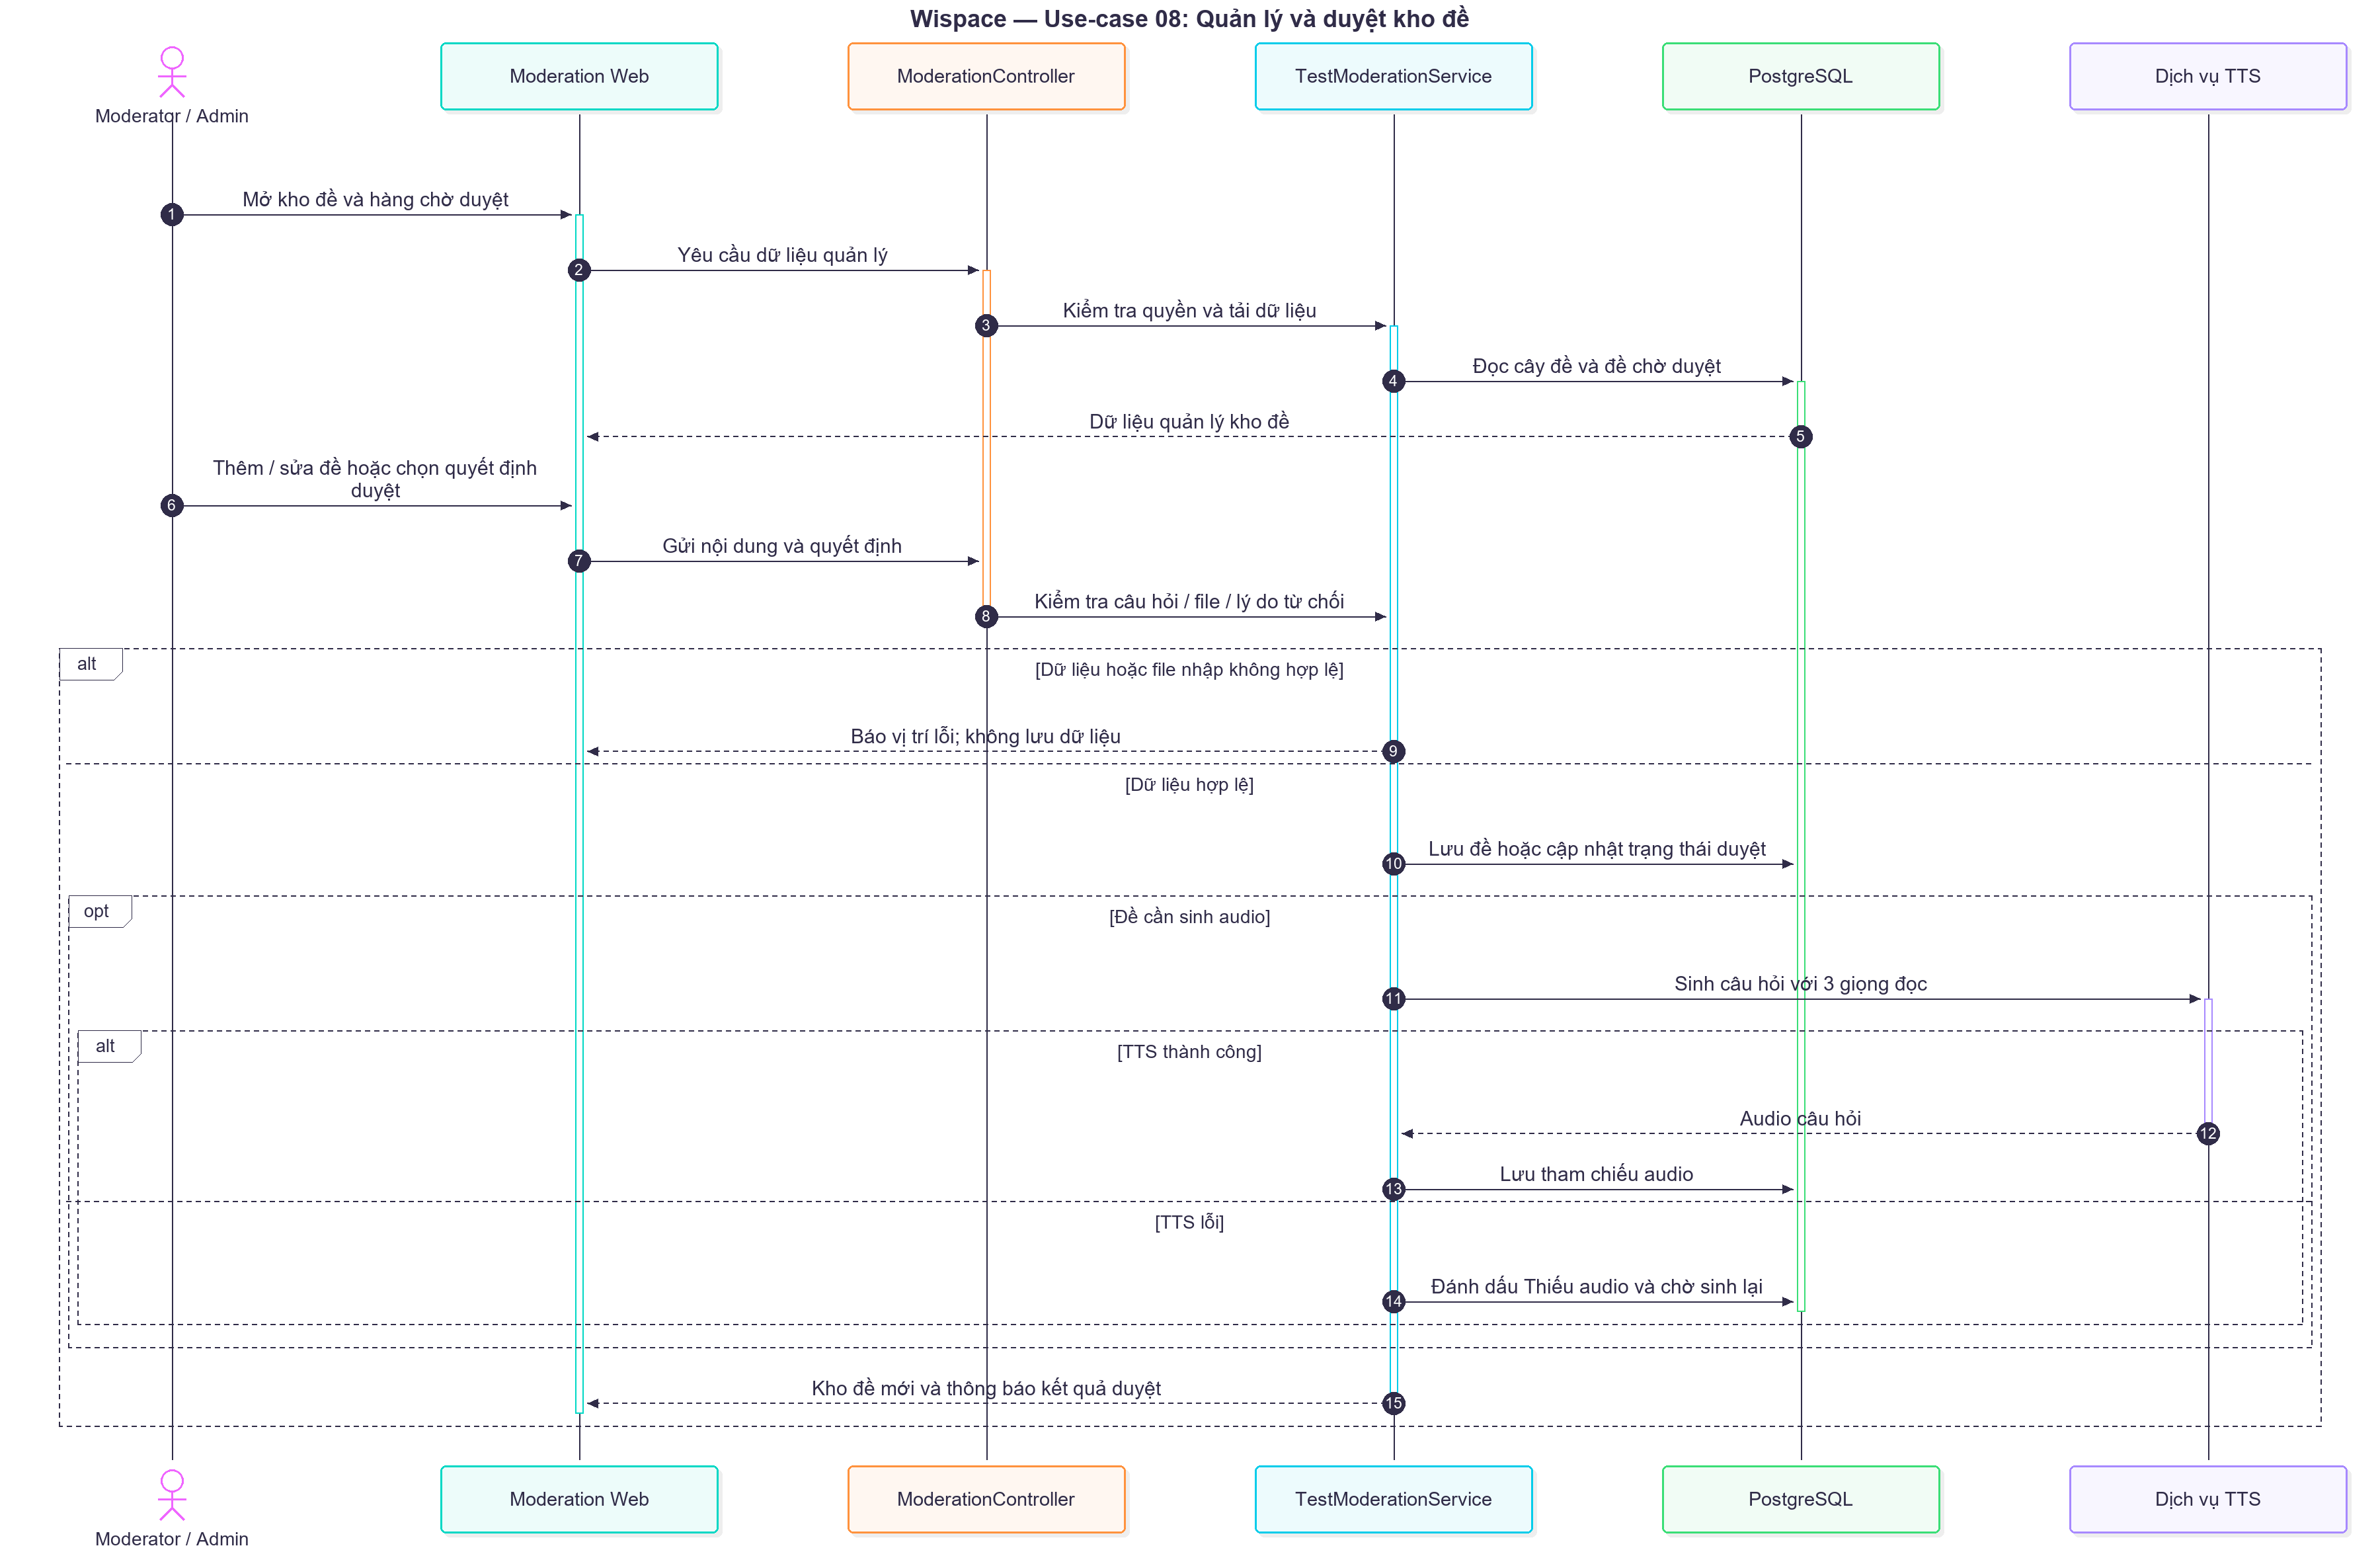
\includegraphics[width=\linewidth,height=.77\textheight,keepaspectratio]{Images/Sequence/Wispace/sequence_uc08_moderate_tests.png}
\caption{Sequence diagram Wispace UC08 — Quản lý và kiểm duyệt đề}
\label{sequence:wispace:sequence_uc08_moderate_tests}
\end{figure}

Quyết định duyệt sử dụng phiên bản để tránh ghi đè; ẩn đề bảo toàn lịch sử của người học.

\clearpage
\paragraph*{UC09. Luyện tập Speaking theo Part}

\begin{figure}[H]
\centering
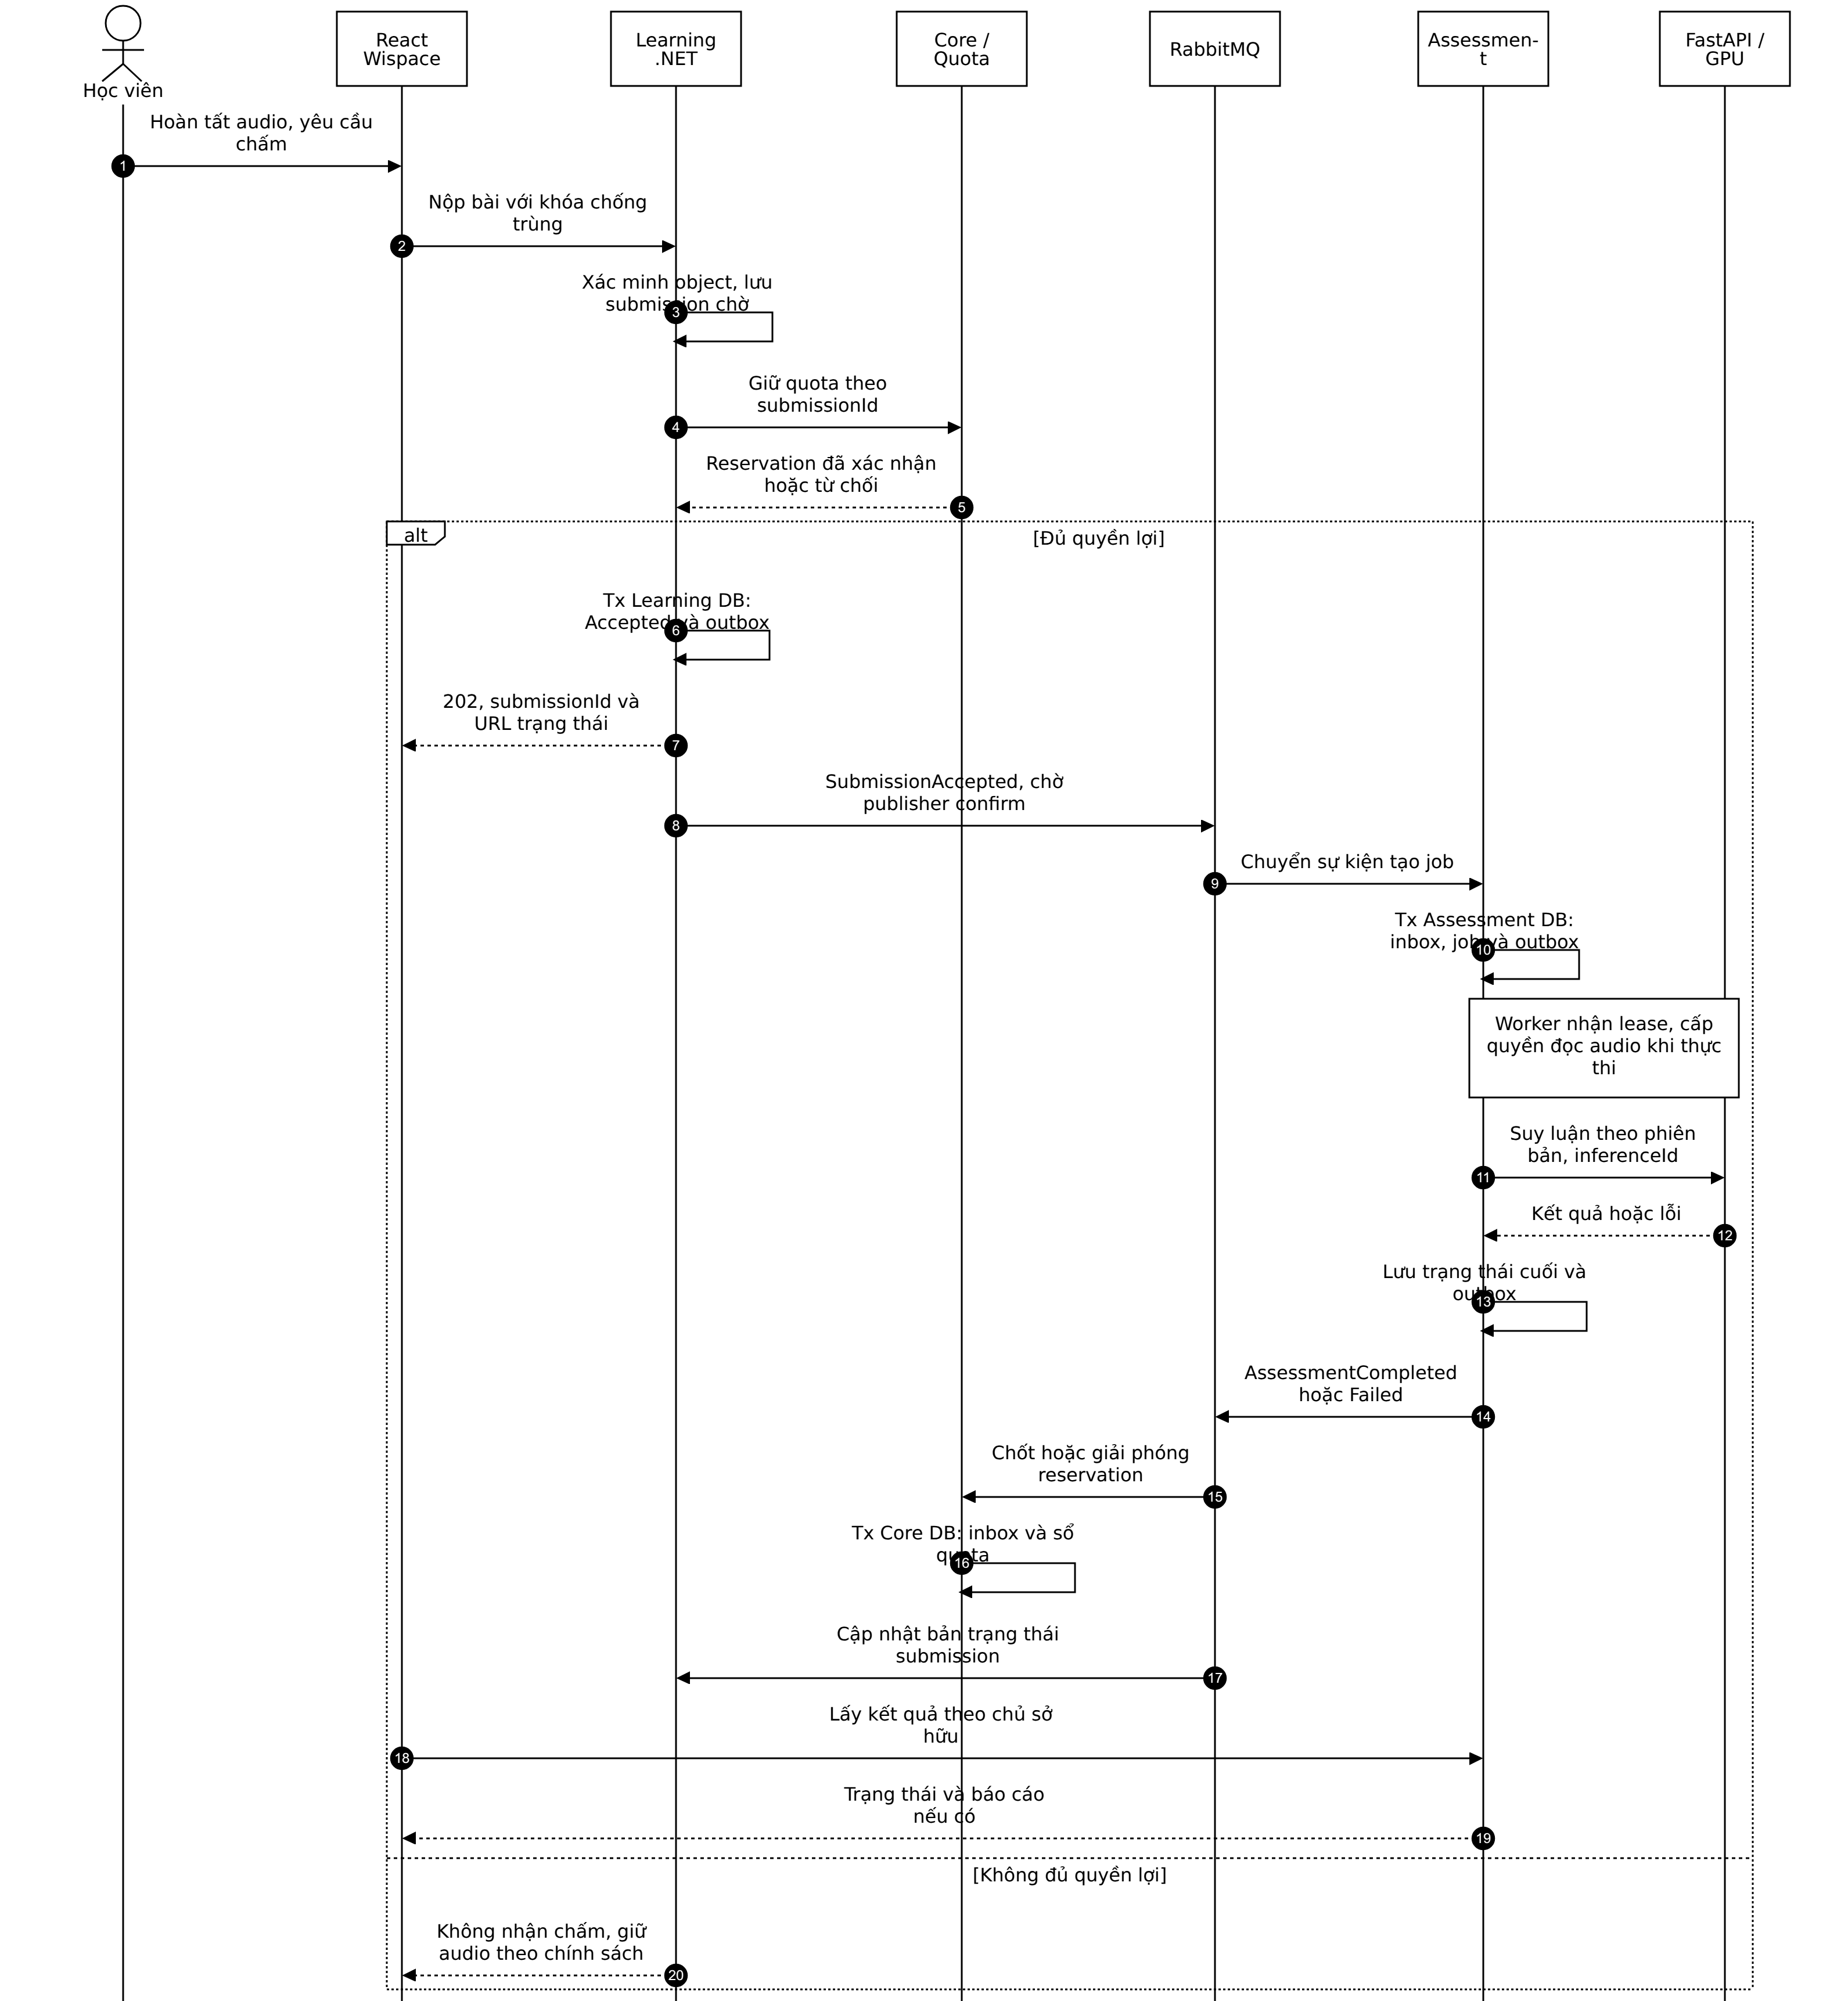
\includegraphics[width=\linewidth,height=.77\textheight,keepaspectratio]{Images/Sequence/Wispace/sequence_uc09_part_practice.png}
\caption{Sequence diagram Wispace UC09 — Luyện tập Speaking theo Part}
\label{sequence:wispace:sequence_uc09_part_practice}
\end{figure}

Learning, Core và Assessment dùng transaction riêng; sự kiện có outbox/inbox, quota không chốt trong transaction của Assessment.

\clearpage
\paragraph*{UC10. Xem kết quả và chấm lại}

\begin{figure}[H]
\centering
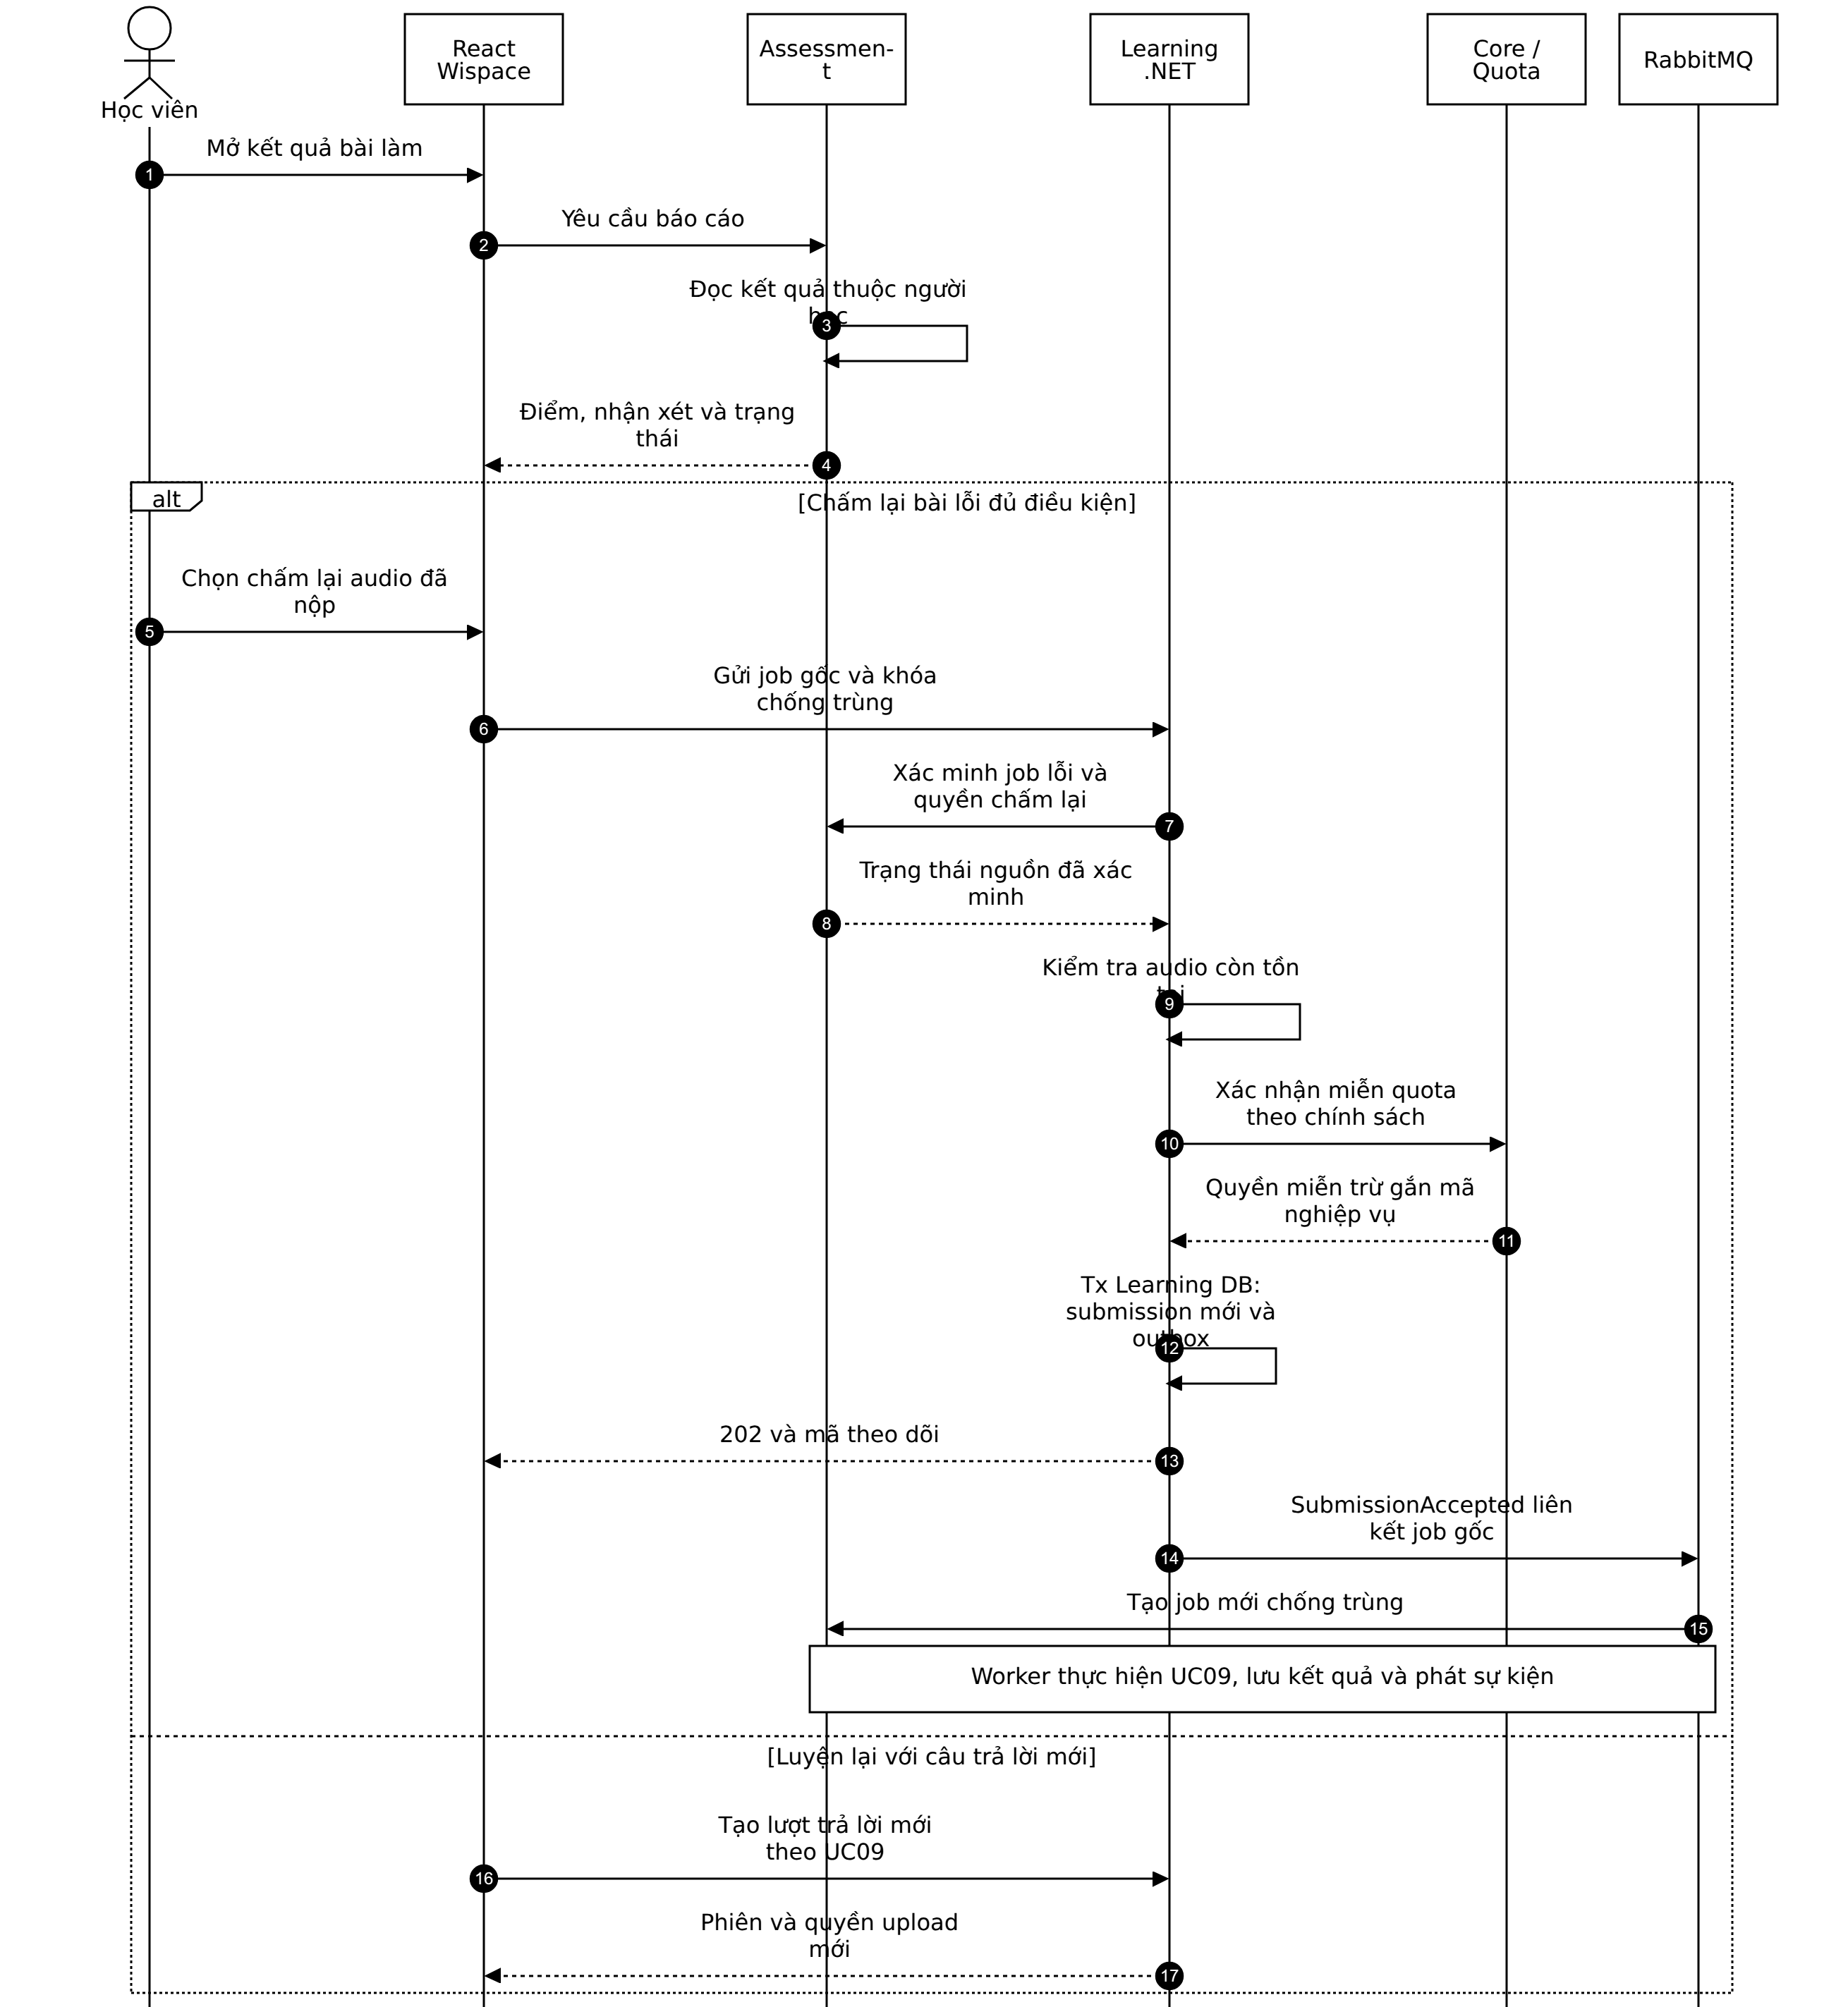
\includegraphics[width=\linewidth,height=.77\textheight,keepaspectratio]{Images/Sequence/Wispace/sequence_uc10_results_retry.png}
\caption{Sequence diagram Wispace UC10 — Xem kết quả và chấm lại}
\label{sequence:wispace:sequence_uc10_results_retry}
\end{figure}

Chấm lại lỗi phải xác minh miễn quota và audio; lượt luyện mới tạo submission mới, không cập nhật trực tiếp sổ Core.

\clearpage
\paragraph*{UC11. Thi thử Speaking}

\begin{figure}[H]
\centering
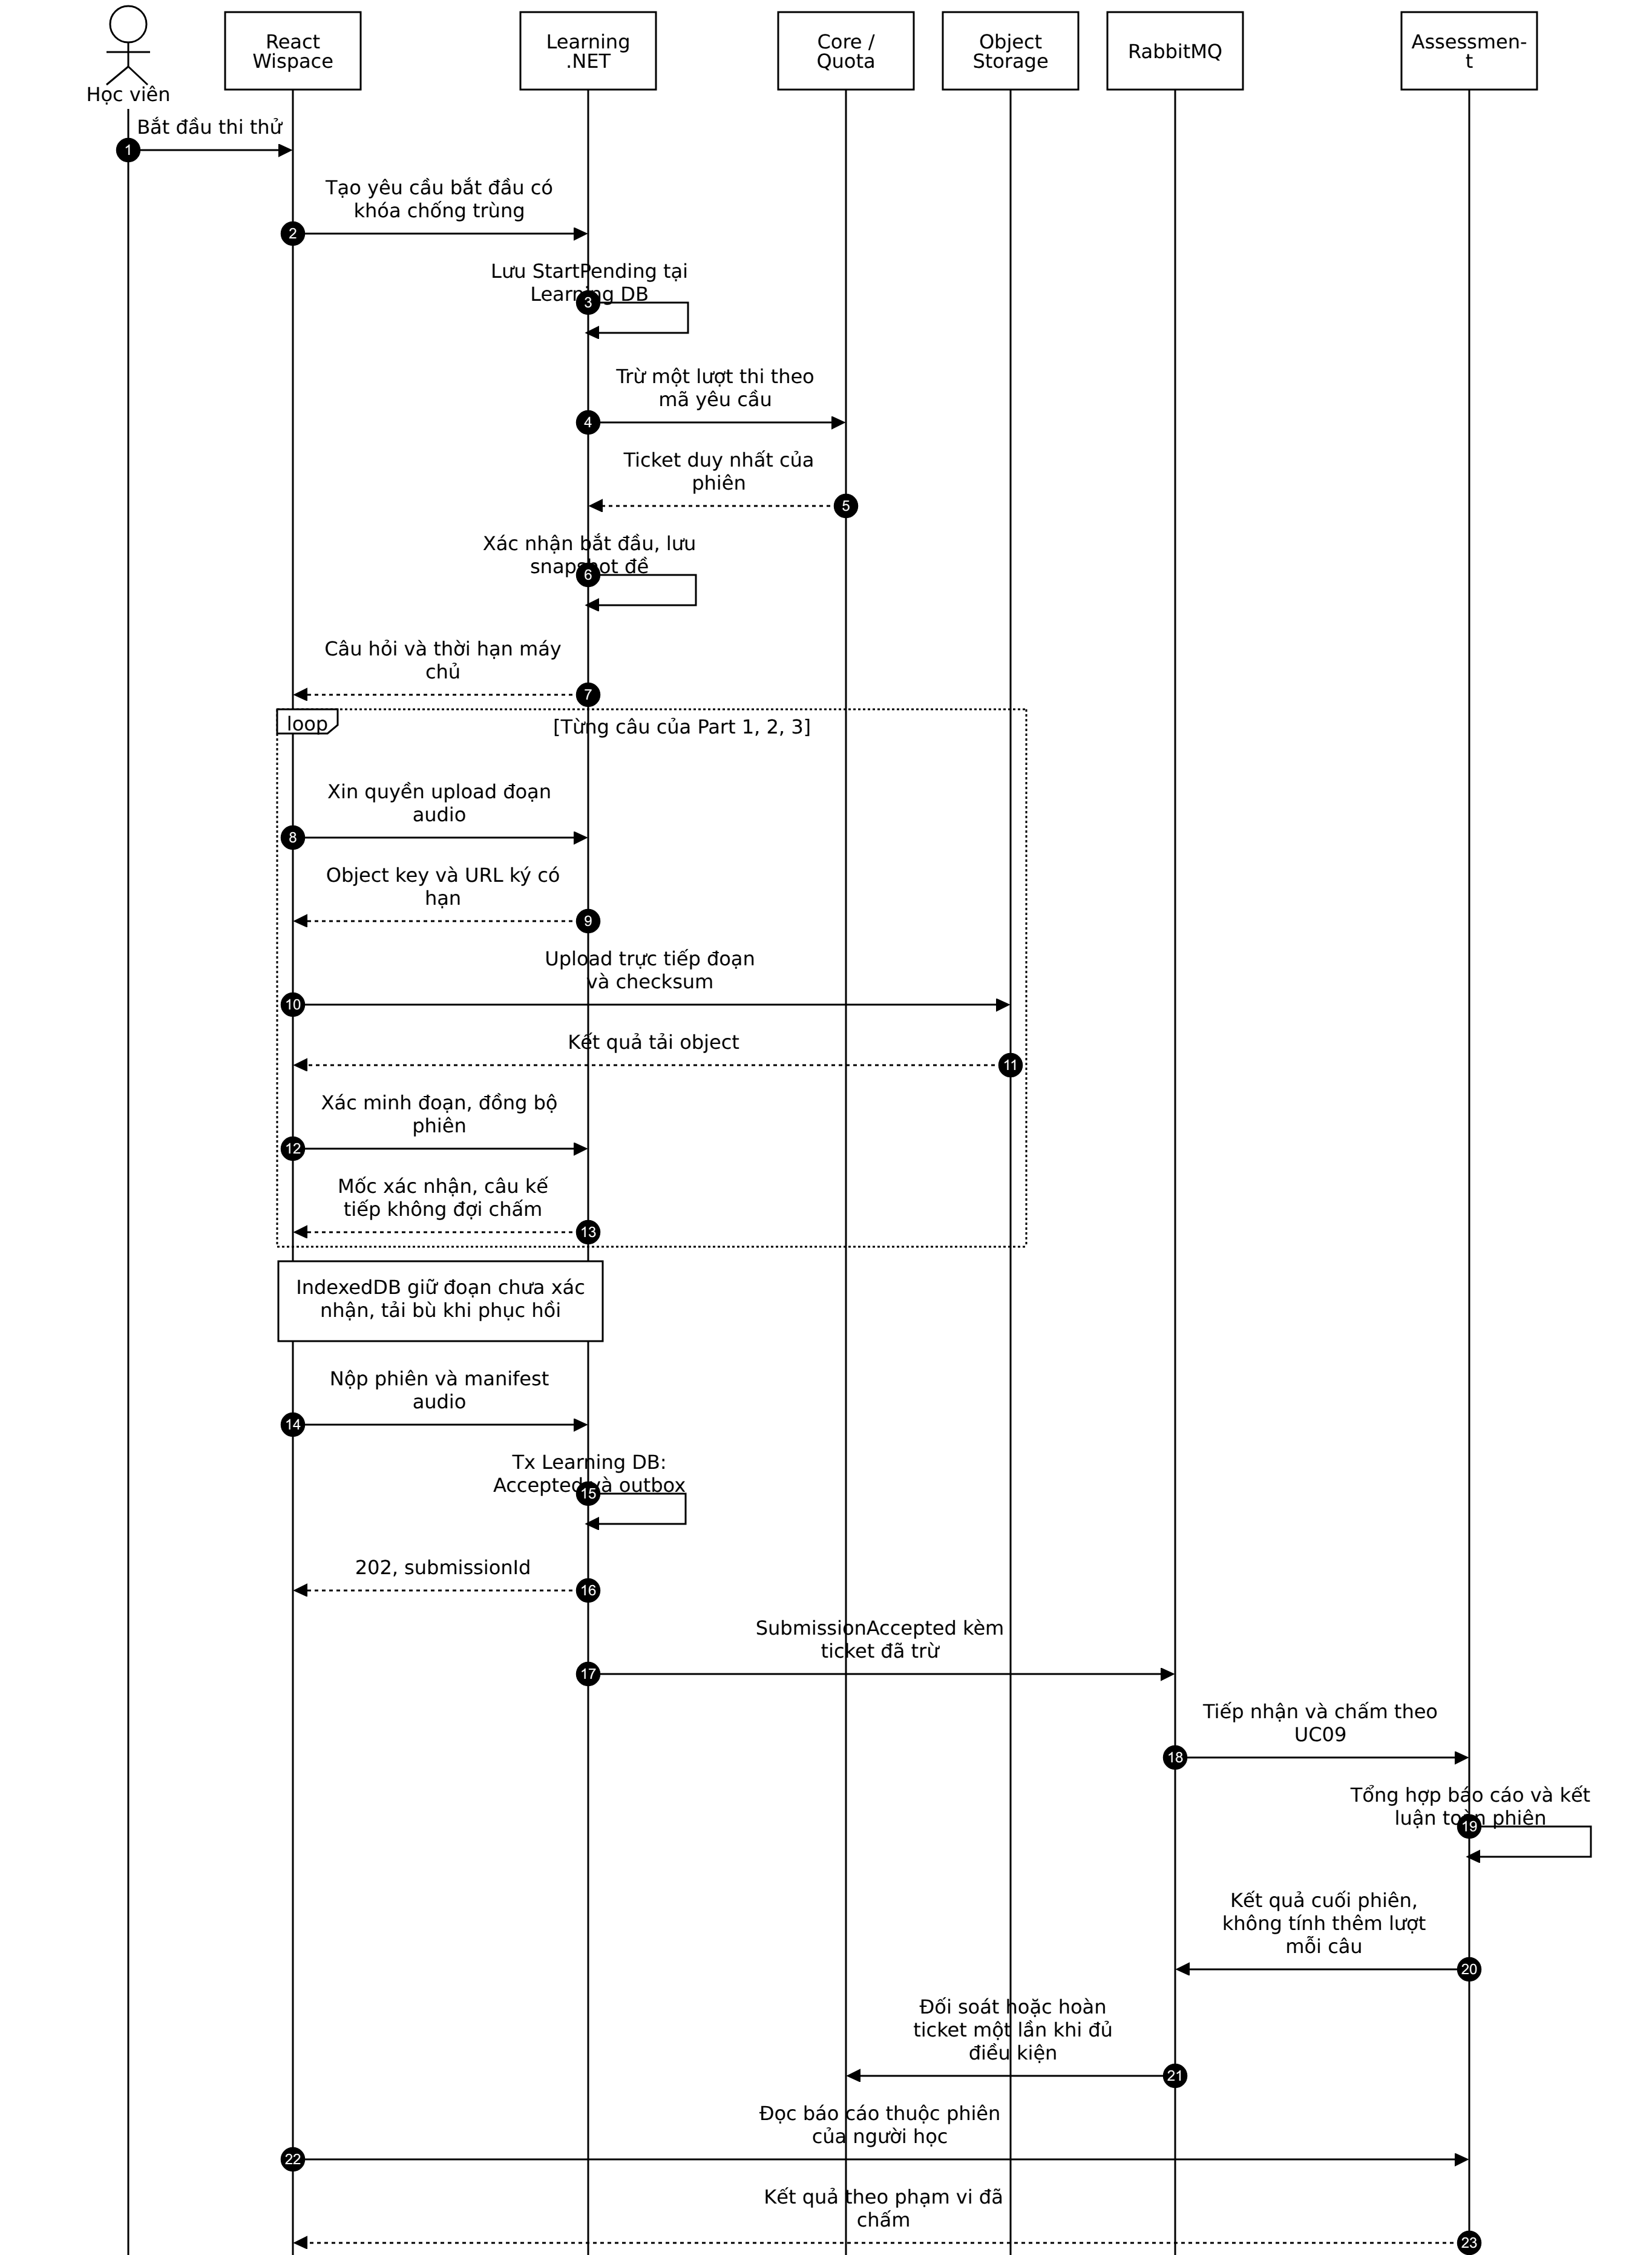
\includegraphics[width=\linewidth,height=.77\textheight,keepaspectratio]{Images/Sequence/Wispace/sequence_uc11_mock_test.png}
\caption{Sequence diagram Wispace UC11 — Thi thử Speaking}
\label{sequence:wispace:sequence_uc11_mock_test}
\end{figure}

Audio đi trực tiếp vào Object Storage; Core trừ một lượt theo ticket, Assessment kết luận toàn phiên trước khi phát quyết định hoàn.

\clearpage
\paragraph*{UC12. Lịch sử và theo dõi tiến bộ}

\begin{figure}[H]
\centering
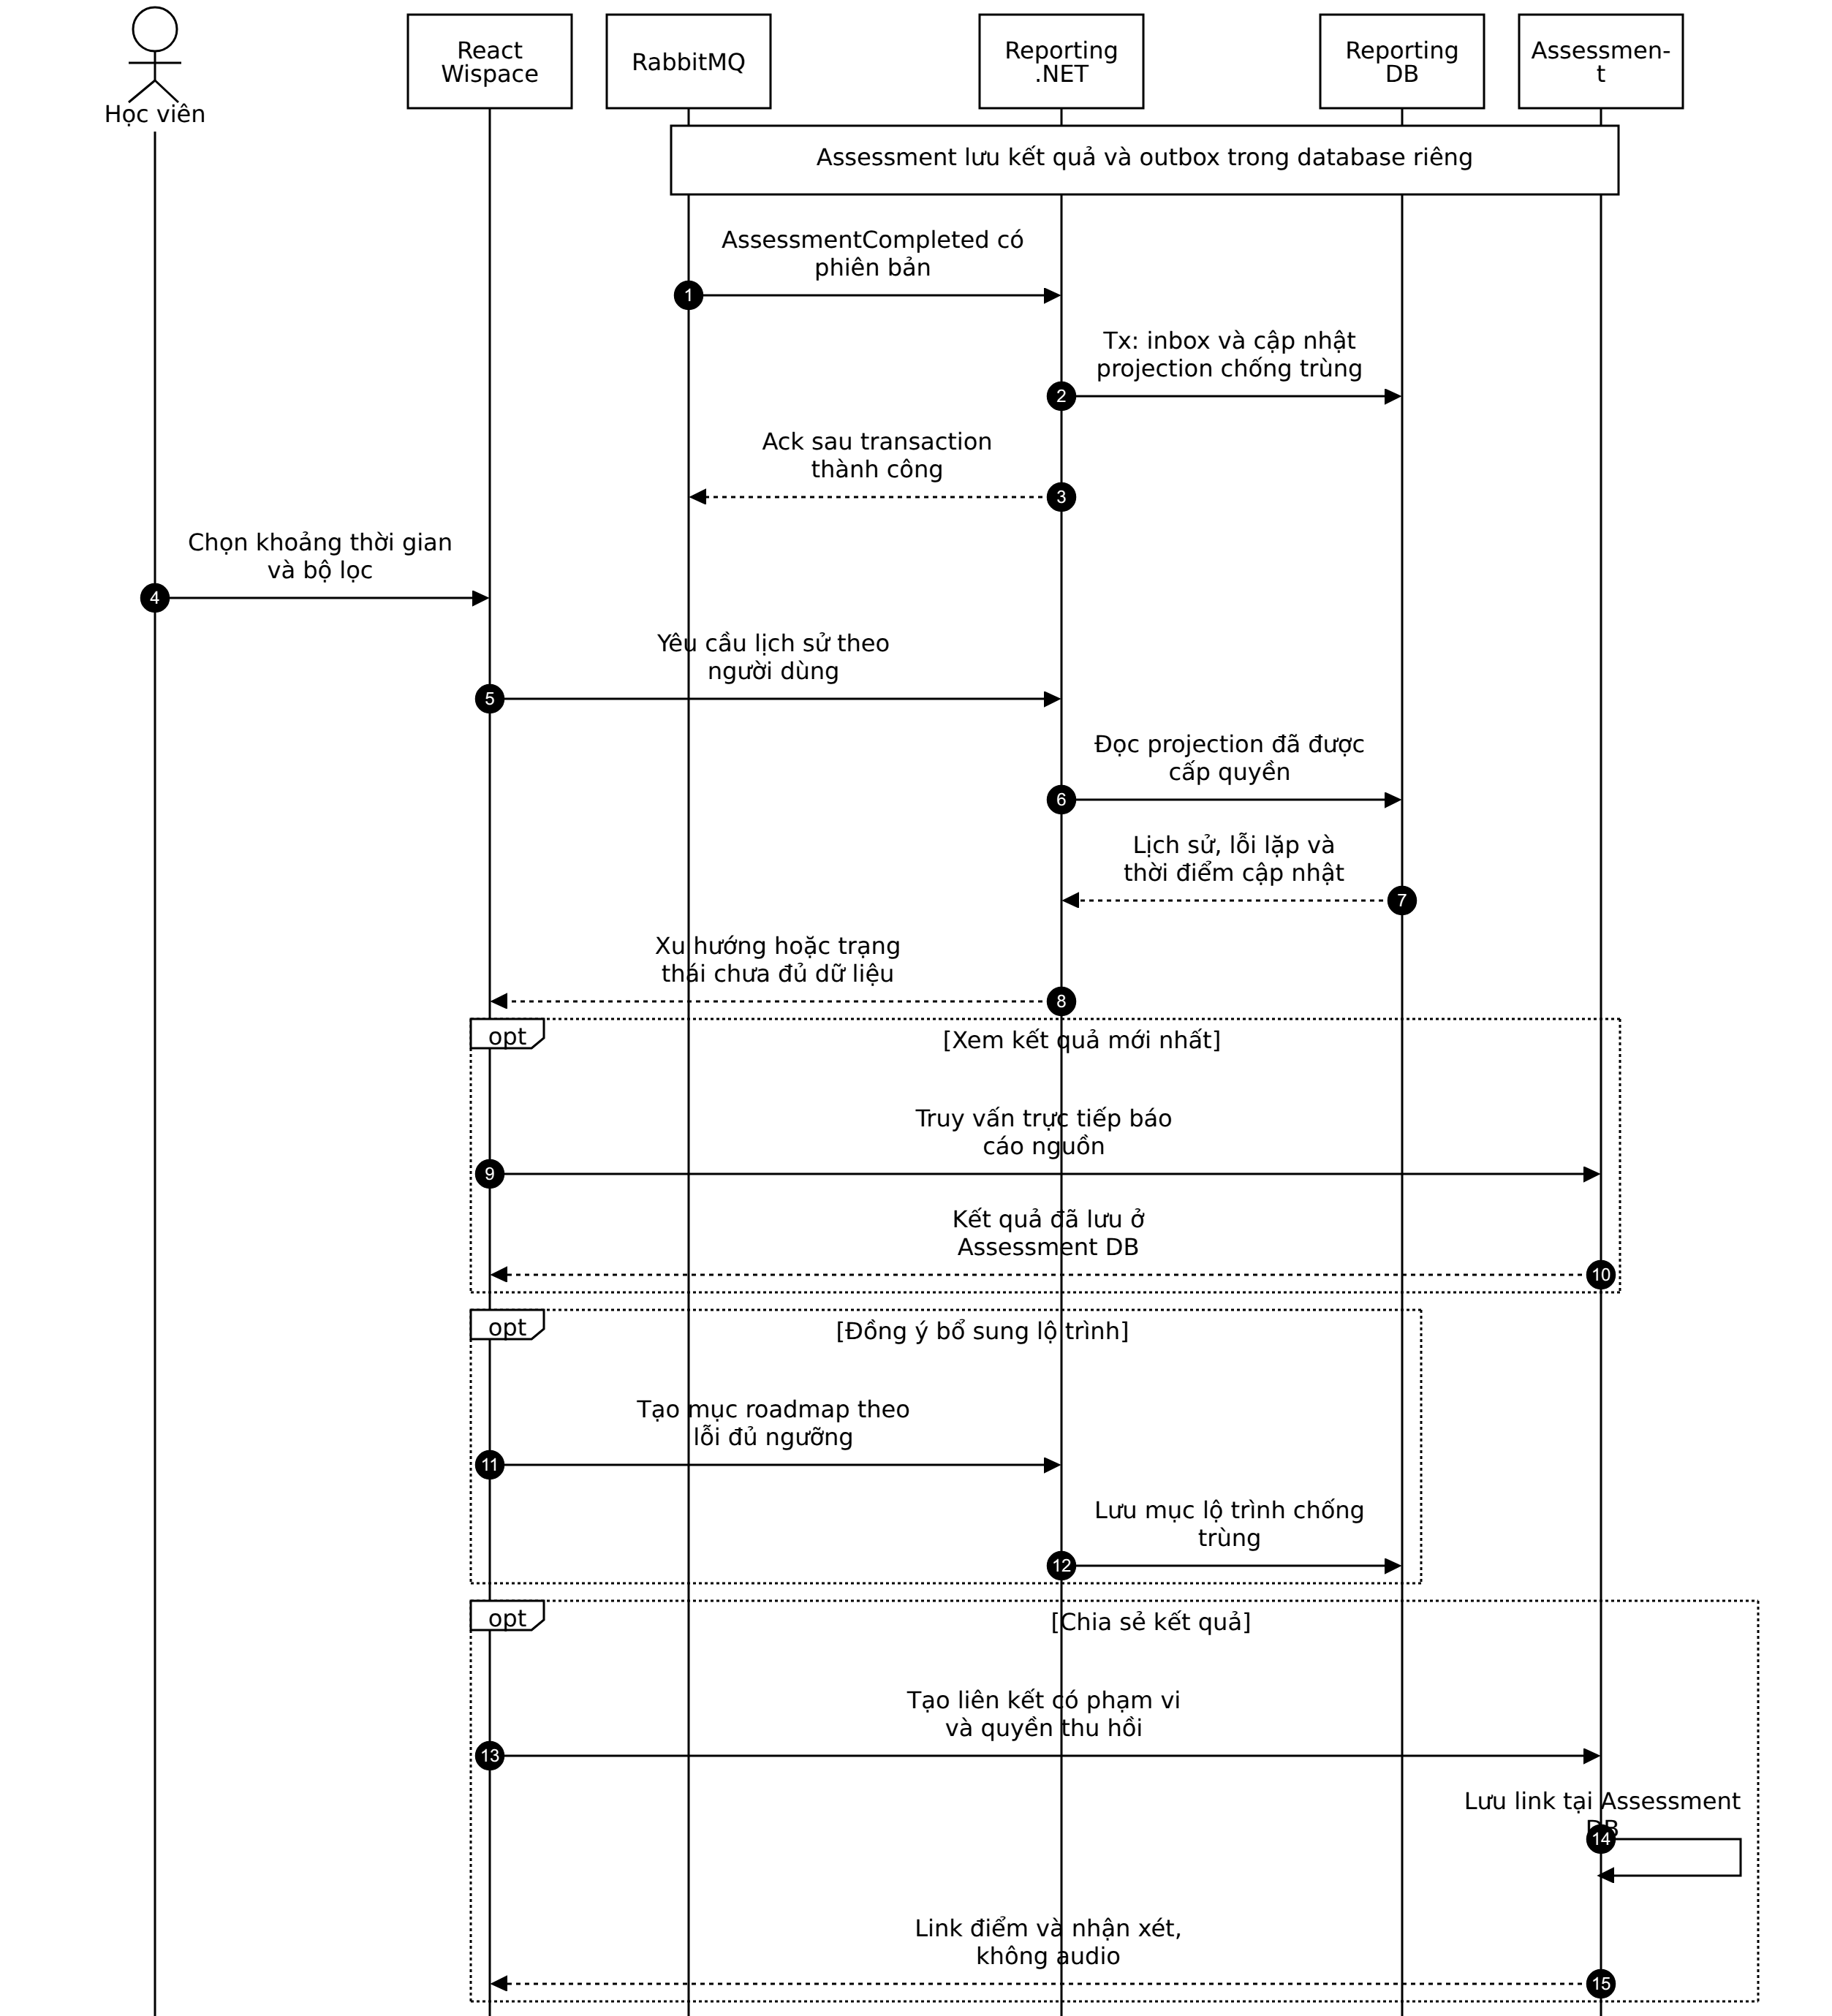
\includegraphics[width=\linewidth,height=.77\textheight,keepaspectratio]{Images/Sequence/Wispace/sequence_uc12_progress_history.png}
\caption{Sequence diagram Wispace UC12 — Lịch sử và theo dõi tiến bộ}
\label{sequence:wispace:sequence_uc12_progress_history}
\end{figure}

Reporting đọc database tổng hợp riêng, hiển thị độ mới dữ liệu; báo cáo nguồn và liên kết chia sẻ thuộc Assessment.

\subsubsection{Bảo mật và vận hành riêng của Wispace}

Quyền truy cập bài làm, audio và kết quả được kiểm tra theo chủ sở hữu tại backend. Moderator được kiểm duyệt kho đề nhưng không mặc nhiên được nghe audio riêng tư của học viên. Link chia sẻ chỉ công bố điểm và nhận xét trong phạm vi được cho phép; học viên có thể thu hồi link.

Luồng chấm dùng queue speaking.assessment và Assessment Worker có giới hạn đồng thời. Kết quả, quota và trạng thái phiên được cập nhật bằng transaction riêng tại dịch vụ sở hữu, kết nối bằng outbox/inbox và cơ chế đối soát. Thông báo SignalR chỉ gửi đến người được phép; khi mất kết nối, giao diện đọc lại trạng thái bằng REST. Audio có vòng đời 180 ngày; xóa audio không làm mất điểm và transcript được phép giữ.

\subsection{Thiết kế hệ thống AIHub}

\subsubsection{Phạm vi, giao diện và kiến trúc}

AIHub là hệ thống quản lý và cung cấp API mô hình cho các tổ chức B2B. Frontend React AIHub phục vụ Portal đối tác, quản trị nền tảng và khu vực Academic Lab nội bộ. Ứng dụng máy chủ của đối tác gọi API B2B trên .NET; Gateway xác thực credentials, kiểm tra quyền dịch vụ và điều phối tới Python FastAPI qua adapter được cấu hình.

AIHub có thể cung cấp cùng mô hình Speaking mà Wispace đang sử dụng, nhưng yêu cầu đối tác có danh tính tổ chức, quota và nhật ký riêng. Các dịch vụ sinh bài tập, Prompt, dẫn chứng và xuất dữ liệu thuộc công cụ chất lượng mô hình; khách B2B không tự động có quyền truy cập dữ liệu Academic Lab.

\paragraph*{Tổ chức frontend}

Frontend AIHub có ba khu vực chức năng:

\begin{enumerate}
\item \textbf{Portal khách hàng B2B:} tổ chức, thành viên, credentials, danh mục API, tài liệu tích hợp, Sandbox, hạn mức và usage.
\item \textbf{Quản trị nền tảng:} danh mục mô hình, model route, gói B2B, cấu hình dịch vụ và giám sát.
\item \textbf{Academic Lab nội bộ:} mẫu sinh, bản hiệu đính, điểm chất lượng, quyết định duyệt và xuất dữ liệu.
\end{enumerate}

Việc tách route trên React giúp tổ chức giao diện. Backend phải kiểm tra quyền độc lập tại từng endpoint; ẩn nút hoặc chặn route phía trình duyệt không thay thế kiểm soát truy cập trên máy chủ.

\begin{figure}[H]
\centering
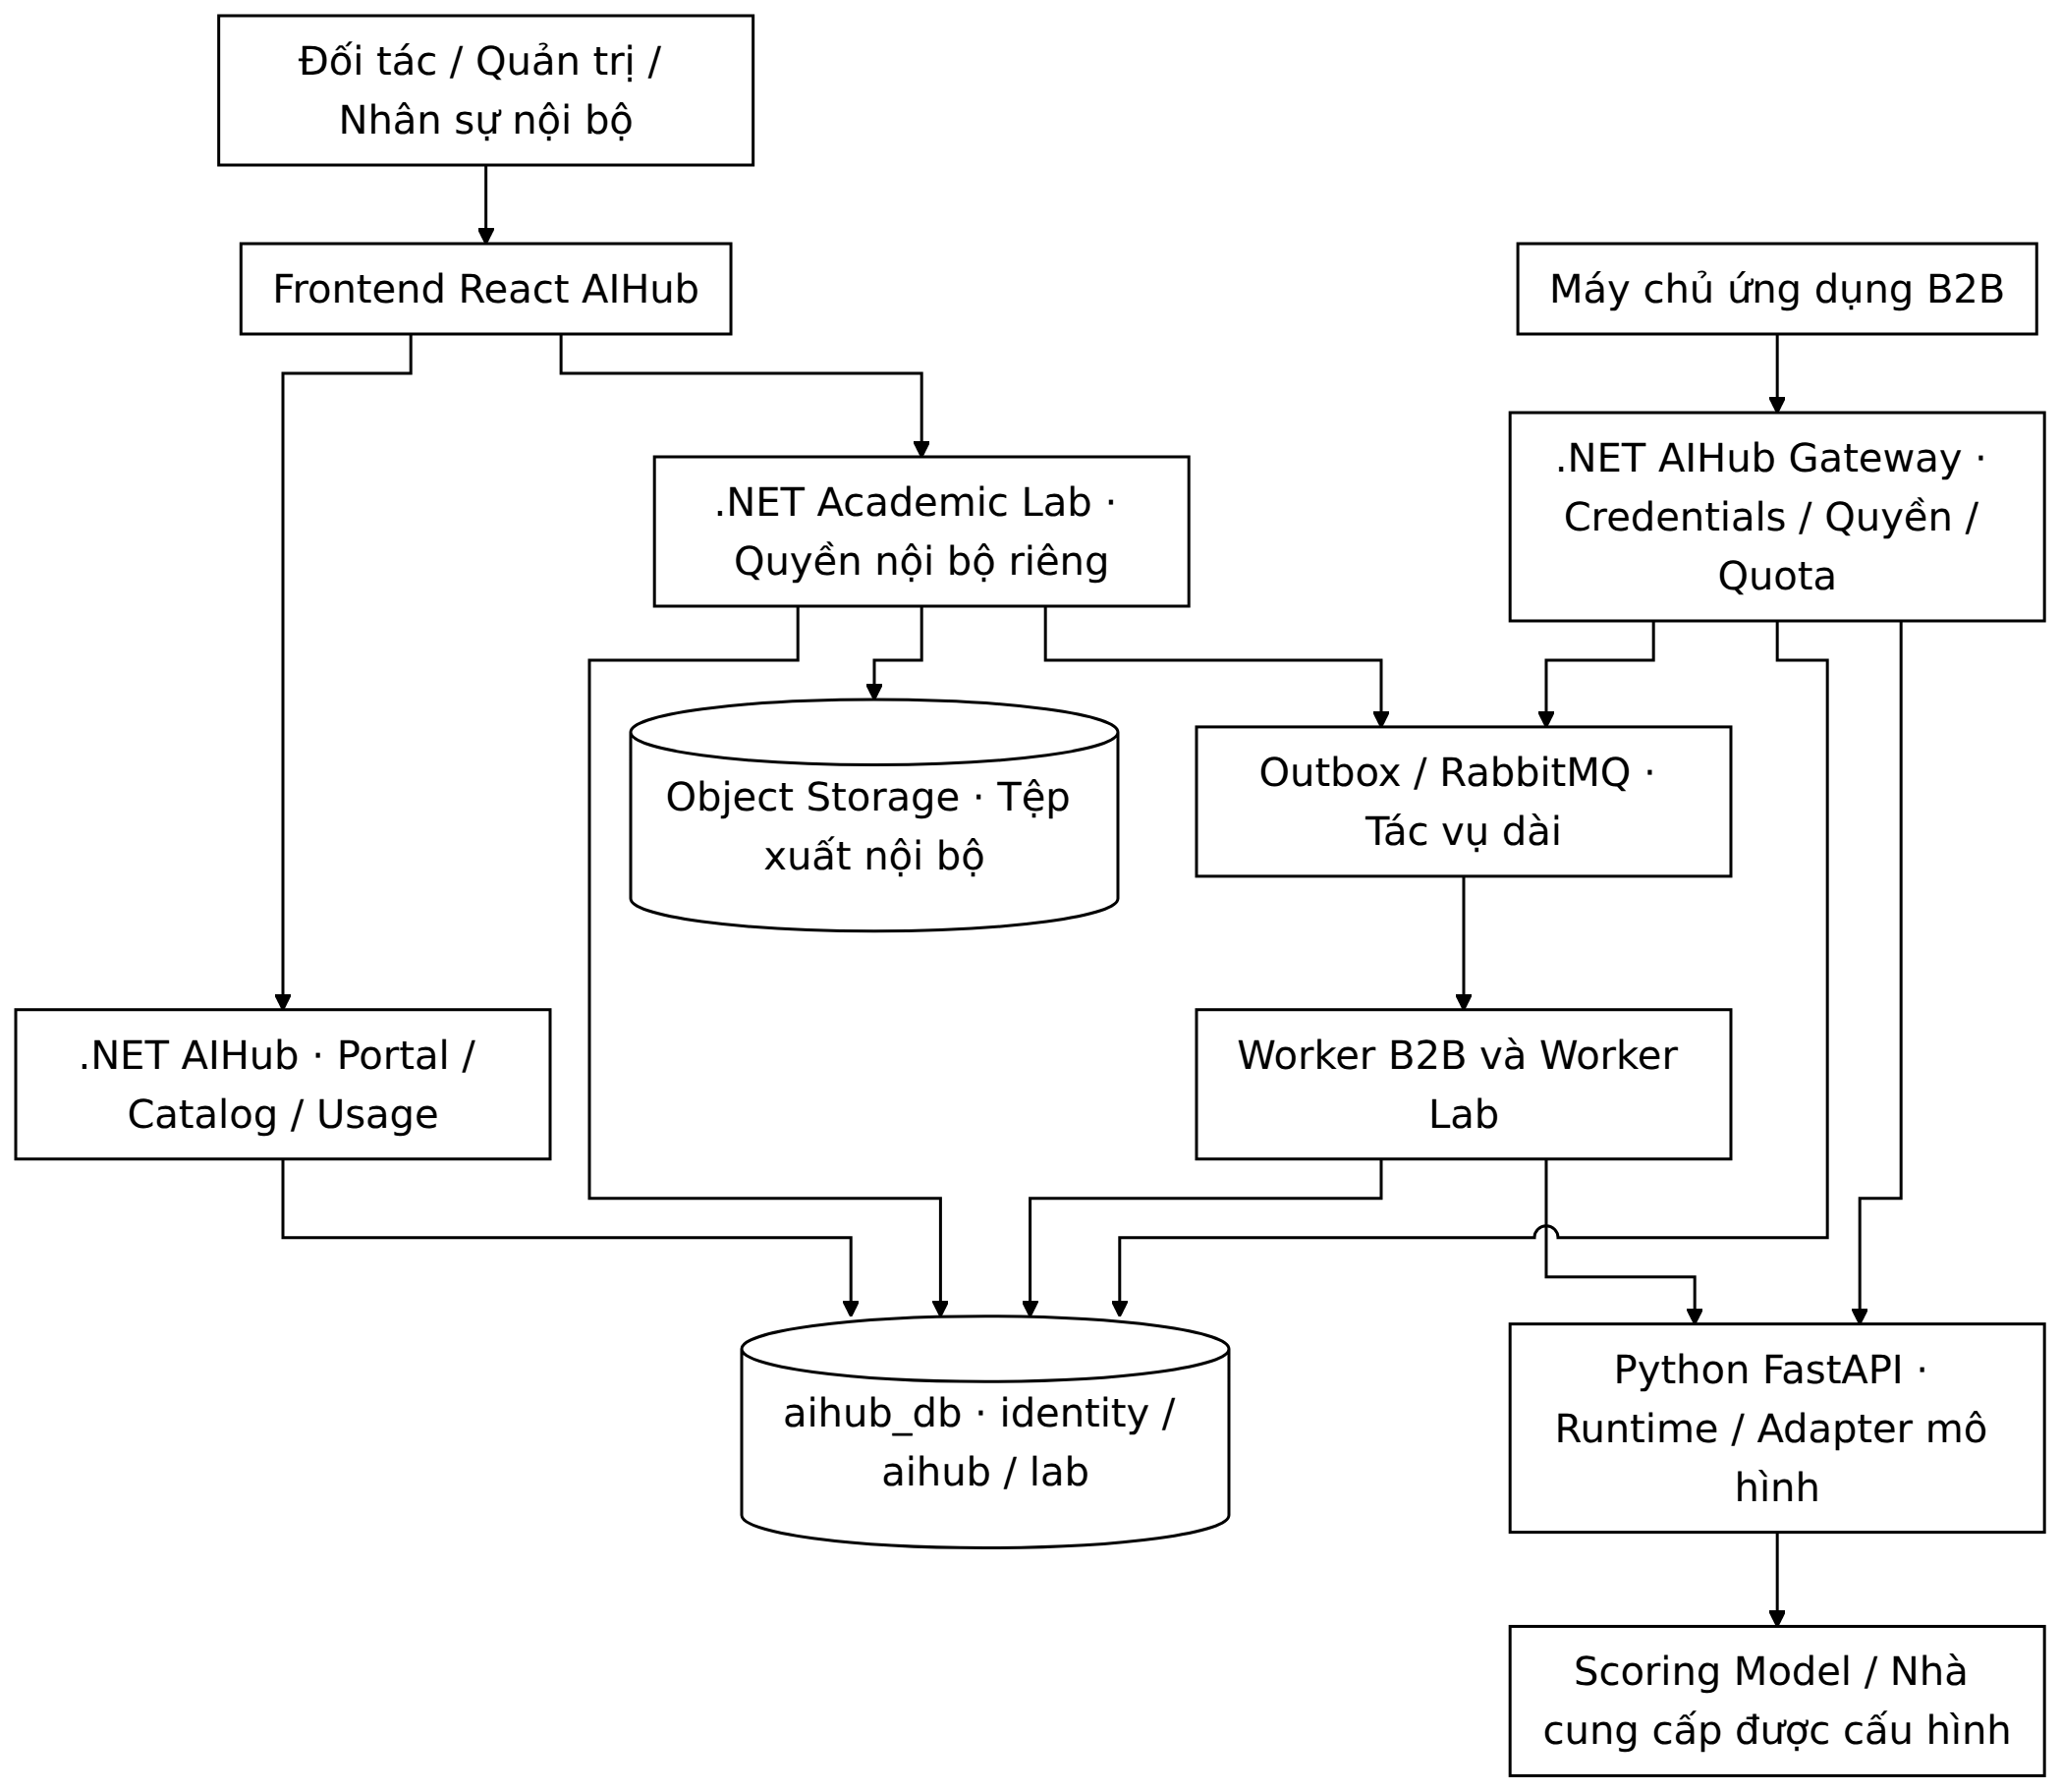
\includegraphics[width=\linewidth,height=.72\textheight,keepaspectratio]{Images/Design/aihub_architecture.png}
\caption{Kiến trúc chức năng của AIHub}
\label{design:fig:aihub_architecture}
\end{figure}

\paragraph*{Các module xử lý}

\begingroup\small\setstretch{1.1}
\begin{longtable}{|>{\raggedright\arraybackslash}p{\dimexpr 0.29\linewidth-2\tabcolsep-2\arrayrulewidth\relax}|>{\raggedright\arraybackslash}p{\dimexpr 0.71\linewidth-2\tabcolsep-2\arrayrulewidth\relax}|}
\caption{Các module xử lý}\label{design:tab:2}\\
\hline
\textbf{Module} & \textbf{Trách nhiệm} \\ \hline
\endfirsthead
\hline
\textbf{Module} & \textbf{Trách nhiệm} \\ \hline
\endhead
\endfoot
AIHub.Access & Tổ chức, thành viên, credentials và quyền dùng dịch vụ. \\ \hline
AIHub.Gateway & Xác thực B2B, kiểm định yêu cầu, điều phối thực thi và chuẩn hóa phản hồi. \\ \hline
AIHub.Catalog & Danh mục API, Universal Specs, phiên bản mô hình, model route và Sandbox. \\ \hline
AIHub.Usage & Gói tổ chức, rate limit, quota, usage và đối soát. \\ \hline
AcademicLab & Dẫn chứng, sinh mẫu, hiệu đính, thẩm định, xuất dữ liệu và phân tích chất lượng. \\ \hline
\end{longtable}
\endgroup

\subsubsection{Thiết kế dữ liệu AIHub}

\begin{figure}[H]
\centering
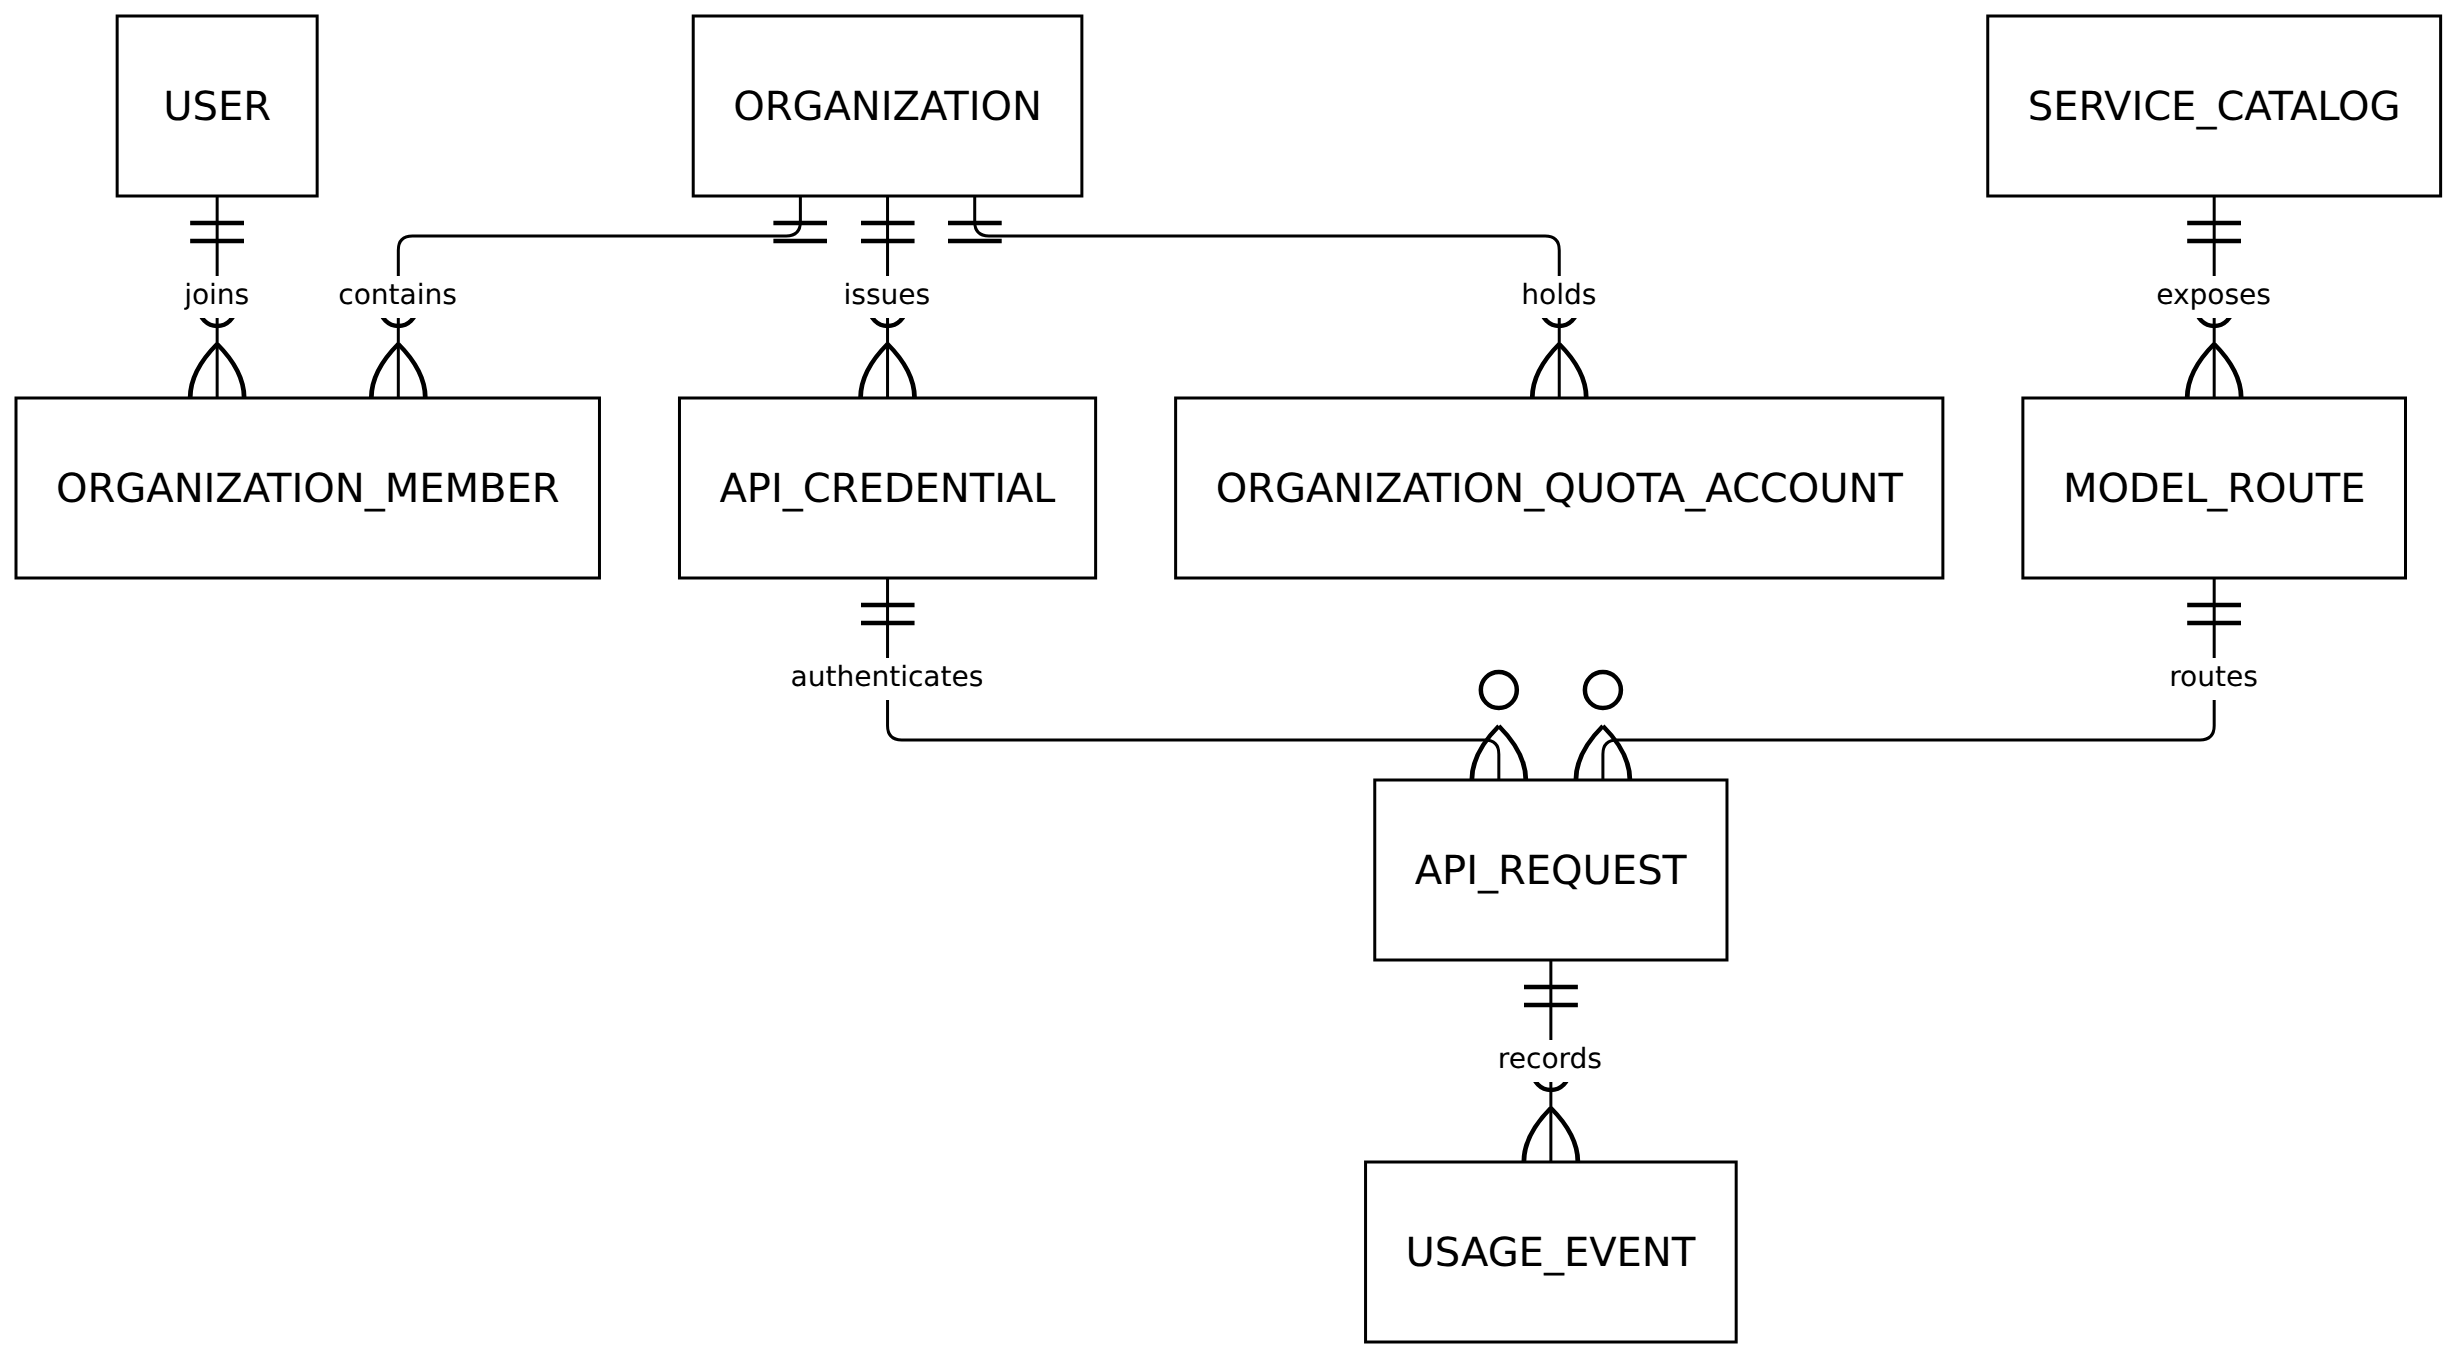
\includegraphics[width=\linewidth,height=.72\textheight,keepaspectratio]{Images/Design/aihub_data.png}
\caption{Quan hệ dữ liệu chính của AIHub B2B}
\label{design:fig:aihub_data}
\end{figure}

\begin{figure}[H]
\centering
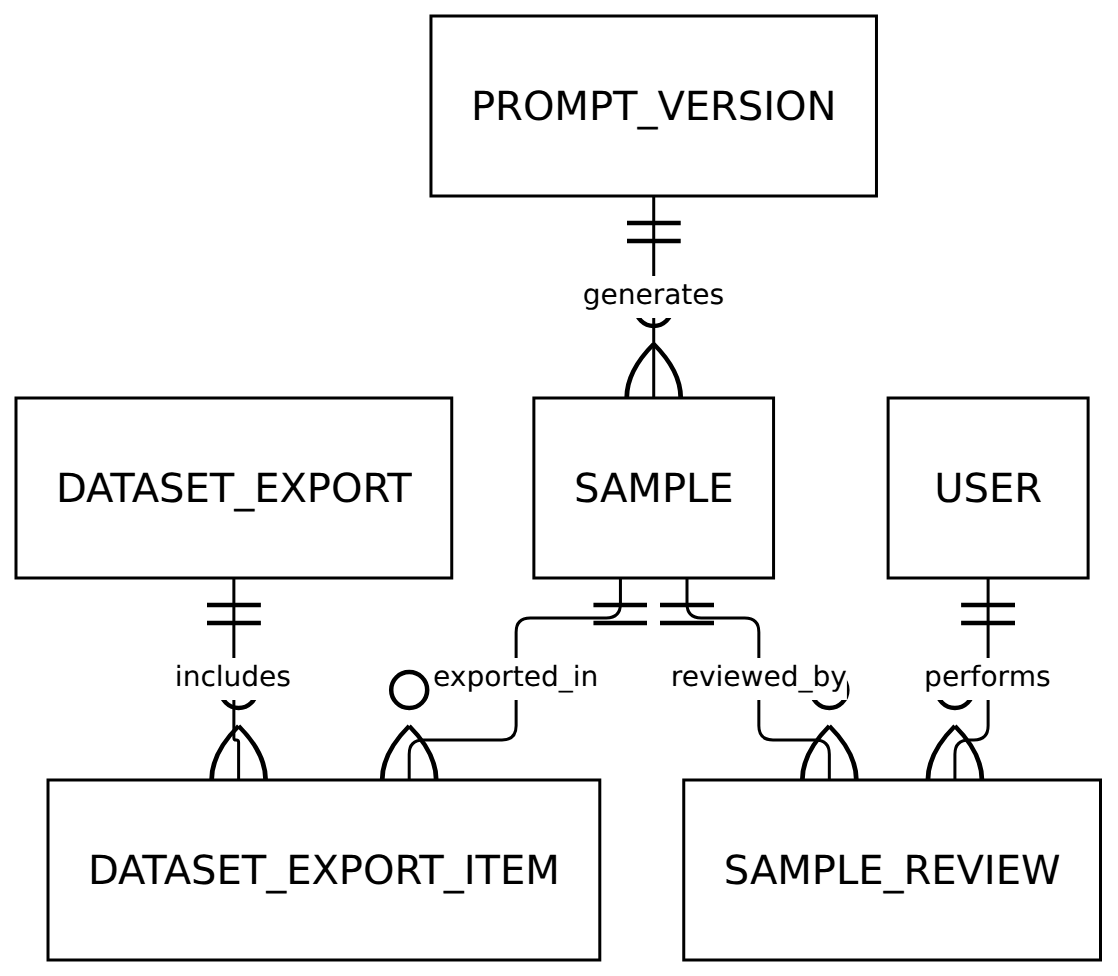
\includegraphics[width=\linewidth,height=.72\textheight,keepaspectratio]{Images/Design/lab_data.png}
\caption{Quan hệ dữ liệu Academic Lab nội bộ}
\label{design:fig:lab_data}
\end{figure}

Một người dùng có thể tham gia nhiều tổ chức. Quyền của thành viên được đánh giá theo tổ chức đang thao tác. Quyền nội bộ của Academic Lab được cấp riêng; việc sở hữu một tổ chức hoặc API key không tạo quyền đọc mẫu, audio hay dữ liệu huấn luyện nội bộ.

Metadata công việc B2B được lưu theo \texttt{api\allowbreak{}Request\allowbreak{}Id} và \texttt{organization\allowbreak{}Id}; những lần thử cần được lưu với route, phiên bản mô hình thực tế, thời gian và lỗi tương ứng. Số liệu chi phí mỗi lần suy luận được tách khỏi số lần tiêu thụ hạn mức nghiệp vụ. Tệp xuất của Academic Lab có manifest riêng, được lưu trong bucket nội bộ với quyền truy cập có thời hạn.

\subsubsection{Thiết kế API B2B và quản lý mô hình}

\paragraph*{Danh mục dịch vụ và quyền khai thác}

AIHub công bố danh mục dịch vụ gồm mã dịch vụ, phiên bản API, schema đầu vào/đầu ra, hình thức xử lý đồng bộ hoặc bất đồng bộ, model route được phép và đơn vị tính hạn mức. Một tổ chức chỉ được gọi các dịch vụ đã được cấp quyền trong gói của mình.

Danh mục có thể bao gồm chấm Speaking hoặc các tác vụ AI khác nếu được cấu hình công khai cho đối tác. Việc công bố cùng một Scoring Model qua B2B không làm thay đổi đường gọi AI trực tiếp của module Wispace. API công khai không cho đối tác truyền tùy ý URL nội bộ, tên container hay địa chỉ nhà cung cấp để backend gọi theo.

\paragraph*{Luồng tiếp nhận API B2B}

\begin{figure}[H]
\centering
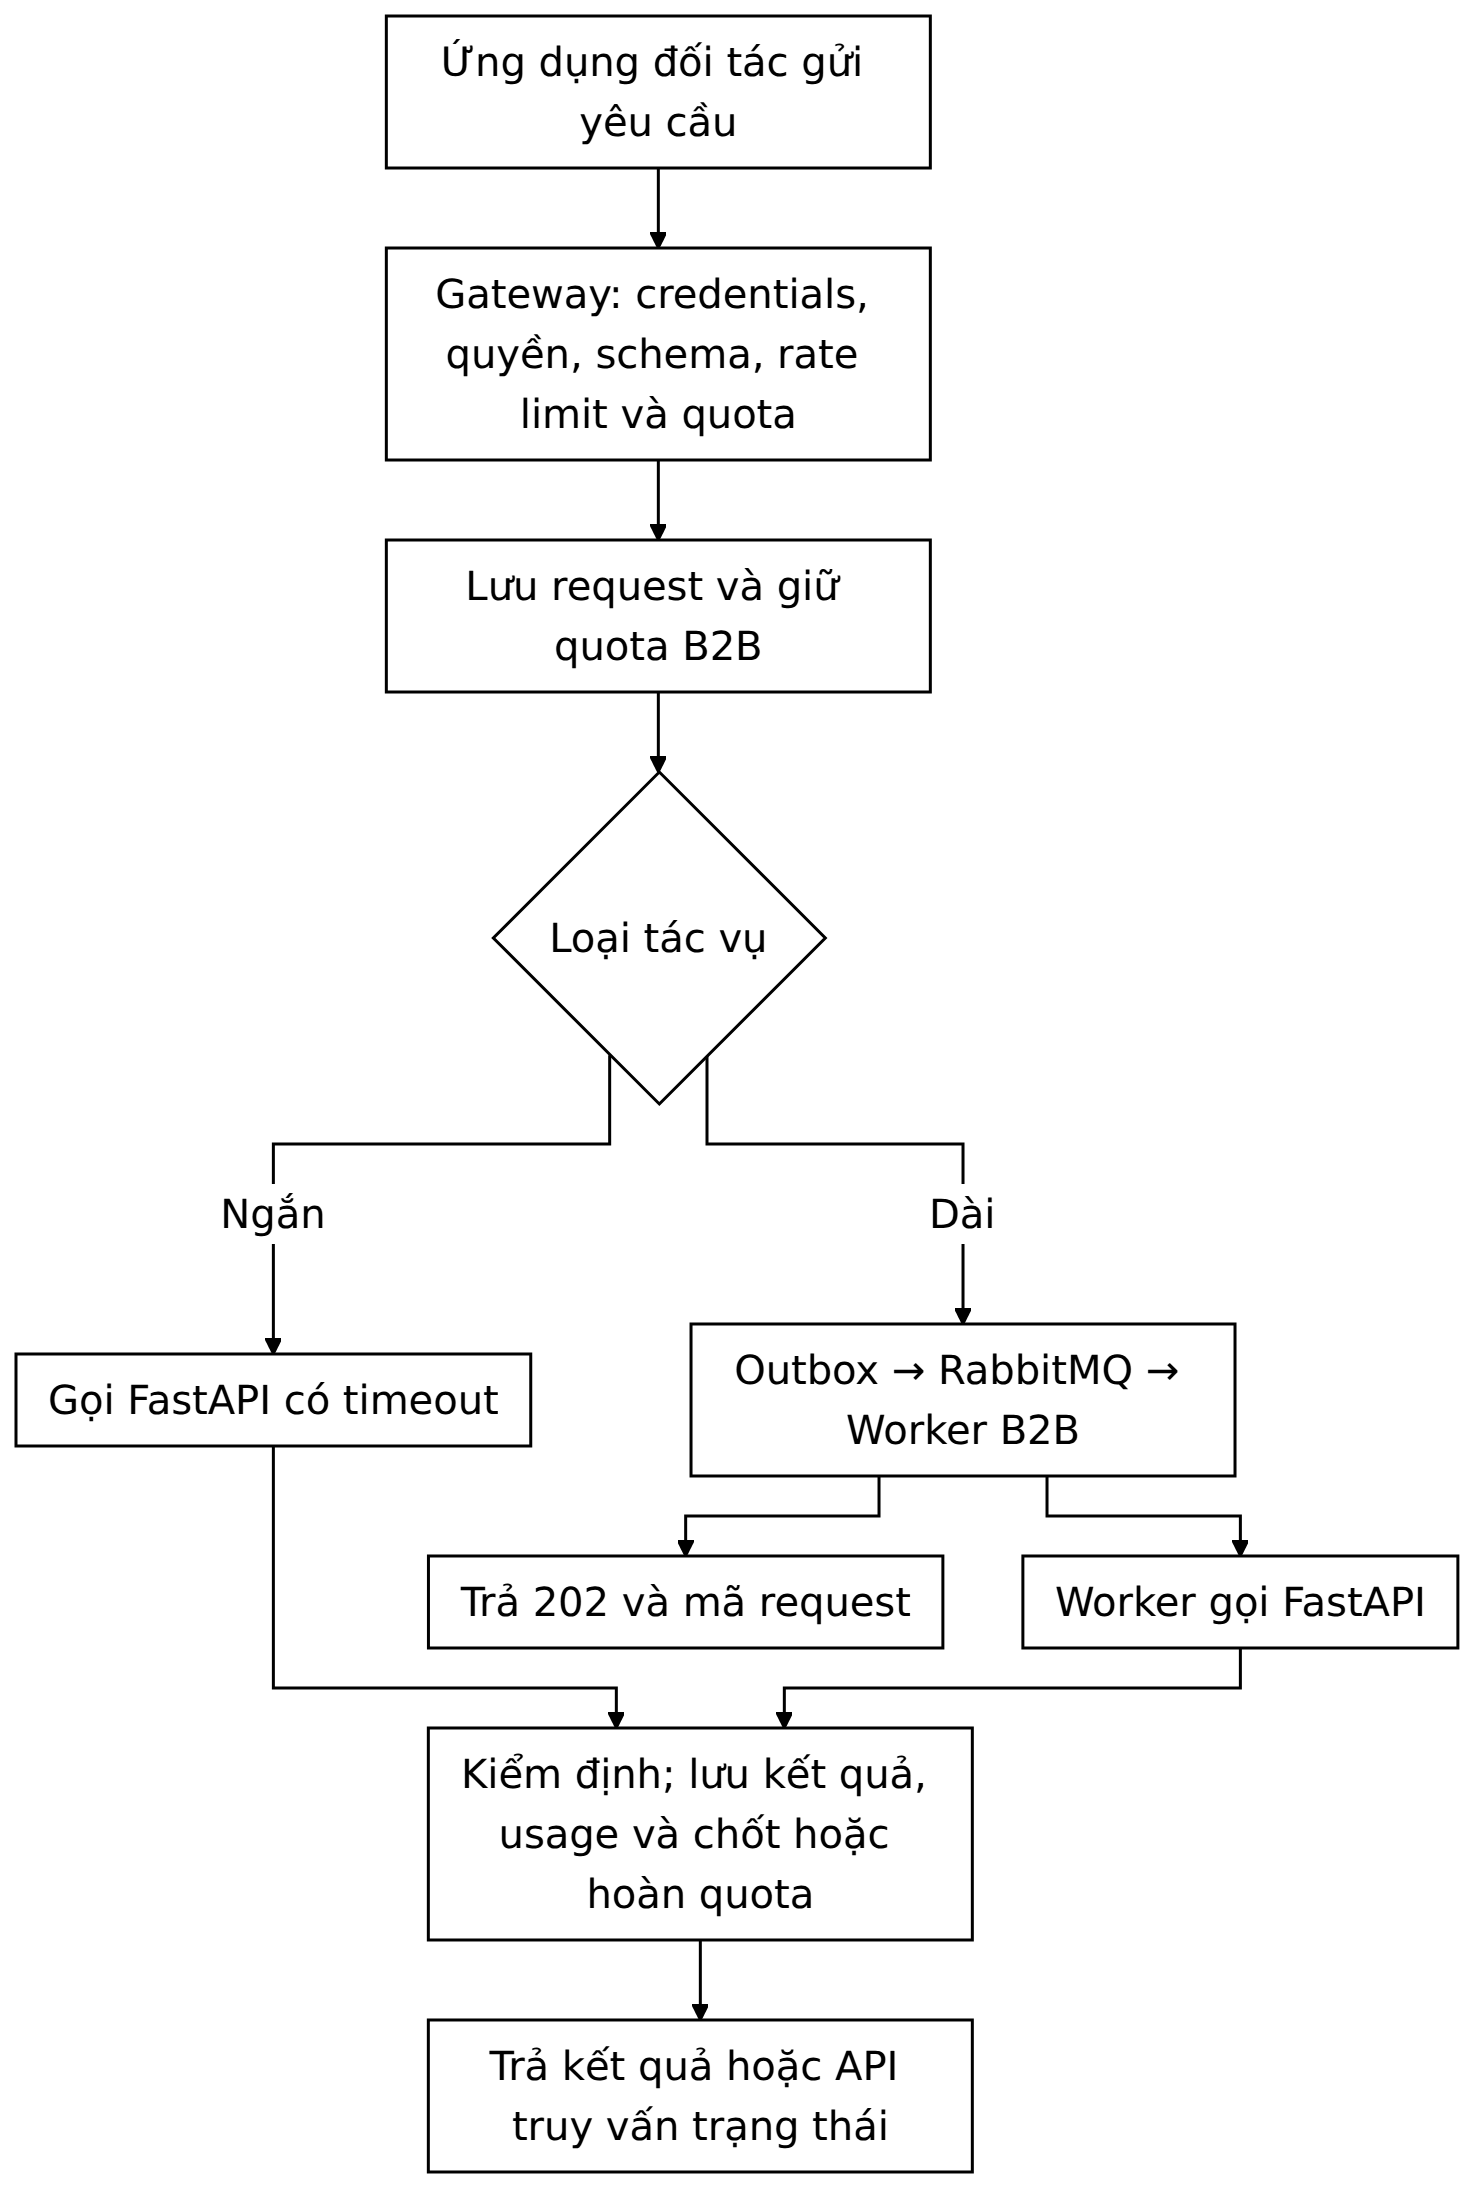
\includegraphics[width=\linewidth,height=.72\textheight,keepaspectratio]{Images/Design/b2b_flow.png}
\caption{Luồng tiếp nhận API B2B}
\label{design:fig:b2b_flow}
\end{figure}

Các tác vụ dài như chấm audio được xử lý bất đồng bộ. Đối tác nhận mã yêu cầu và dùng endpoint truy vấn trạng thái trong phạm vi tổ chức. Những tác vụ ngắn có thể dùng phản hồi đồng bộ với timeout phù hợp. Nếu client gửi lại do mất phản hồi, \texttt{Idempotency-\allowbreak{}Key} và nội dung yêu cầu phải được kiểm tra để tránh tạo yêu cầu và tính hạn mức lặp.

\paragraph*{Credentials và phân quyền tổ chức}

Mỗi bộ credentials có \texttt{client\allowbreak{}Id}, bí mật ngẫu nhiên, môi trường sử dụng, tập quyền dịch vụ, thời điểm tạo và trạng thái. Bí mật chỉ hiển thị một lần khi cấp mới hoặc xoay vòng; hệ thống lưu dạng băm và không cung cấp endpoint đọc lại bí mật gốc.

Đề xuất giữ cách xác thực \texttt{x-\allowbreak{}client-\allowbreak{}id} và \texttt{x-\allowbreak{}secret-\allowbreak{}key} đã được mô tả trong yêu cầu. Credentials được dùng qua HTTPS từ ứng dụng máy chủ của đối tác; không nhúng bí mật B2B vào mã JavaScript công khai. Sau xác thực, \texttt{organization\allowbreak{}Id} được suy ra từ khóa đã lưu, thay vì tin trực tiếp định danh tổ chức trong request body.

Quản trị viên tổ chức có thể quản lý credentials và thành viên trong phạm vi quyền được cấp. Quản trị viên nền tảng mới được công bố dịch vụ, đổi cấu hình model route hoặc thay đổi chính sách gói toàn cục. Khóa bị thu hồi phải bị từ chối ở các yêu cầu tiếp theo theo kiểm tra trạng thái có thẩm quyền; cache xác thực không được làm vô hiệu thao tác thu hồi.

\paragraph*{Rate limit, quota và usage}

Rate limit giới hạn tốc độ truy cập trong một khoảng ngắn; quota giới hạn lượng sử dụng theo gói và chu kỳ. Mỗi dịch vụ định nghĩa đơn vị tiêu thụ, ví dụ lượt gọi hoặc thời lượng audio. Việc kiểm tra và giữ quota được thực hiện nguyên tử để các yêu cầu đồng thời không cùng tiêu thụ một số dư.

Thiết kế đề xuất chốt hạn mức nghiệp vụ khi kết quả được lưu thành công; lỗi hệ thống cuối cùng giải phóng phần đang giữ. Các chi phí thực tế của nhà cung cấp, kể cả chi phí phát sinh ở lần thử lỗi, được ghi riêng cho vận hành. Rate limit vẫn ghi nhận lần truy cập để ngăn việc gửi lặp gây quá tải.

Yêu cầu đồng bộ cũng có trạng thái và thời hạn xử lý trong PostgreSQL. Nếu API host dừng giữa lúc gọi mô hình và lưu kết quả, tác vụ đối soát phát hiện yêu cầu quá hạn, kiểm tra kết quả theo định danh khi dịch vụ hỗ trợ, rồi kết thúc hoặc khôi phục theo chính sách. Không tự động gọi lại dịch vụ có tính phí khi chưa xác định hành vi chống lặp; kết quả muộn chỉ được chấp nhận khi yêu cầu vẫn còn quyền hoàn tất. Mọi khoản giữ hạn mức phải được chốt hoặc giải phóng bằng thao tác có kiểm tra chống lặp.

Mỗi usage event chứa tổ chức, credentials, dịch vụ, phiên bản mô hình, request ID, trạng thái, latency và đơn vị tiêu thụ. Với dịch vụ LLM có thể ghi token; với Scoring Model cần ghi thời lượng audio và thời gian suy luận tương ứng. Phân biệt số liệu đo được với chi phí ước tính theo bảng giá cấu hình.

\paragraph*{Chọn mô hình và xử lý dự phòng}

Mỗi loại dịch vụ có chính sách model route riêng. Dịch vụ sinh bài hoặc sinh nội dung có thể sử dụng chuỗi WISPACE Micro-Engine, Gemini, OpenAI và phương án xác định theo cấu hình của đề tài. Đầu ra dự phòng phải được kiểm định theo cùng hợp đồng; phản hồi ghi rõ mô hình thực tế đã sử dụng.

Đối với chấm Speaking, phương án khôi phục là chuyển tới bản sao hoặc phiên bản Scoring Model đã được kiểm chứng, hoặc giữ công việc chờ phục hồi. Chuỗi LLM sinh nội dung không được mặc định sử dụng để thay thế Scoring Model. Khi không có mô hình chấm phù hợp, hệ thống trả trạng thái chờ, không sẵn sàng hoặc thất bại theo loại yêu cầu.

\subsubsection{Thiết kế Academic Lab nội bộ}

Academic Lab được đặt trong khu vực nội bộ của frontend AIHub và có module xử lý riêng trên backend. Module hỗ trợ sinh mẫu từ Prompt có phiên bản, xem đầu ra gốc, hiệu đính, đánh giá chất lượng, chấp thuận/từ chối và phân tích nhóm lỗi. Chỉ nhân sự được cấp quyền nội bộ mới truy cập dữ liệu và thao tác xuất tập huấn luyện.

Mỗi mẫu lưu \texttt{raw\allowbreak{}Ai\allowbreak{}Output}, \texttt{final\allowbreak{}Output}, phiên bản Prompt, mô hình sinh, tiêu chí đánh giá và lịch sử review. Auto-save chỉ lưu bản hiệu đính; quyết định chấp thuận hoặc từ chối là thao tác riêng. Khi phát hiện phiên bản đã bị người khác sửa, backend trả xung đột để người dùng tải dữ liệu mới trước khi tiếp tục.

Việc xuất SFT lấy Prompt và đầu ra đã thẩm định theo schema huấn luyện được chọn. Việc xuất DPO cần cặp \texttt{chosen} và \texttt{rejected} cùng Prompt, có nguồn gốc và tiêu chí lựa chọn rõ ràng. Hai mẫu khác trạng thái không tự tạo thành một cặp hợp lệ. Mỗi lần xuất có manifest ghi danh sách mẫu, phiên bản, bộ lọc, người thực hiện và checksum của tệp.

Dữ liệu Academic Lab phục vụ cải thiện chất lượng mô hình nhưng được phân tách theo nhiệm vụ. Mẫu Writing và nội dung LLM không được coi là dữ liệu nhãn chuẩn để huấn luyện chấm Speaking nếu chưa có quy trình chuyển đổi và gán nhãn phù hợp. Audio dùng để cải thiện Scoring Model phải có sự đồng ý tương ứng và quy trình đánh giá bởi chuyên gia.

Huấn luyện được thực hiện ngoài luồng xử lý API thời gian thực. Artifact sau huấn luyện trải qua đánh giá và đăng ký phiên bản trước khi được đưa vào môi trường suy luận. Một tệp SFT/DPO được xuất thành công không đồng nghĩa mô hình mới đủ điều kiện triển khai.

\subsubsection{Sequence diagram các chức năng AIHub}

Các sơ đồ UC01–UC05 thể hiện Portal và khai thác dịch vụ; UC06–UC15 thể hiện công cụ học thuật/cấu hình nội bộ; UC16–UC20 thể hiện quản trị và vận hành. Nhãn tác nhân trong từng sơ đồ xác định vai trò được phép thực hiện, không xem tài khoản đối tác là quyền truy cập nội bộ.

\clearpage
\paragraph*{UC01. Xác thực Developer Portal}

\begin{figure}[H]
\centering
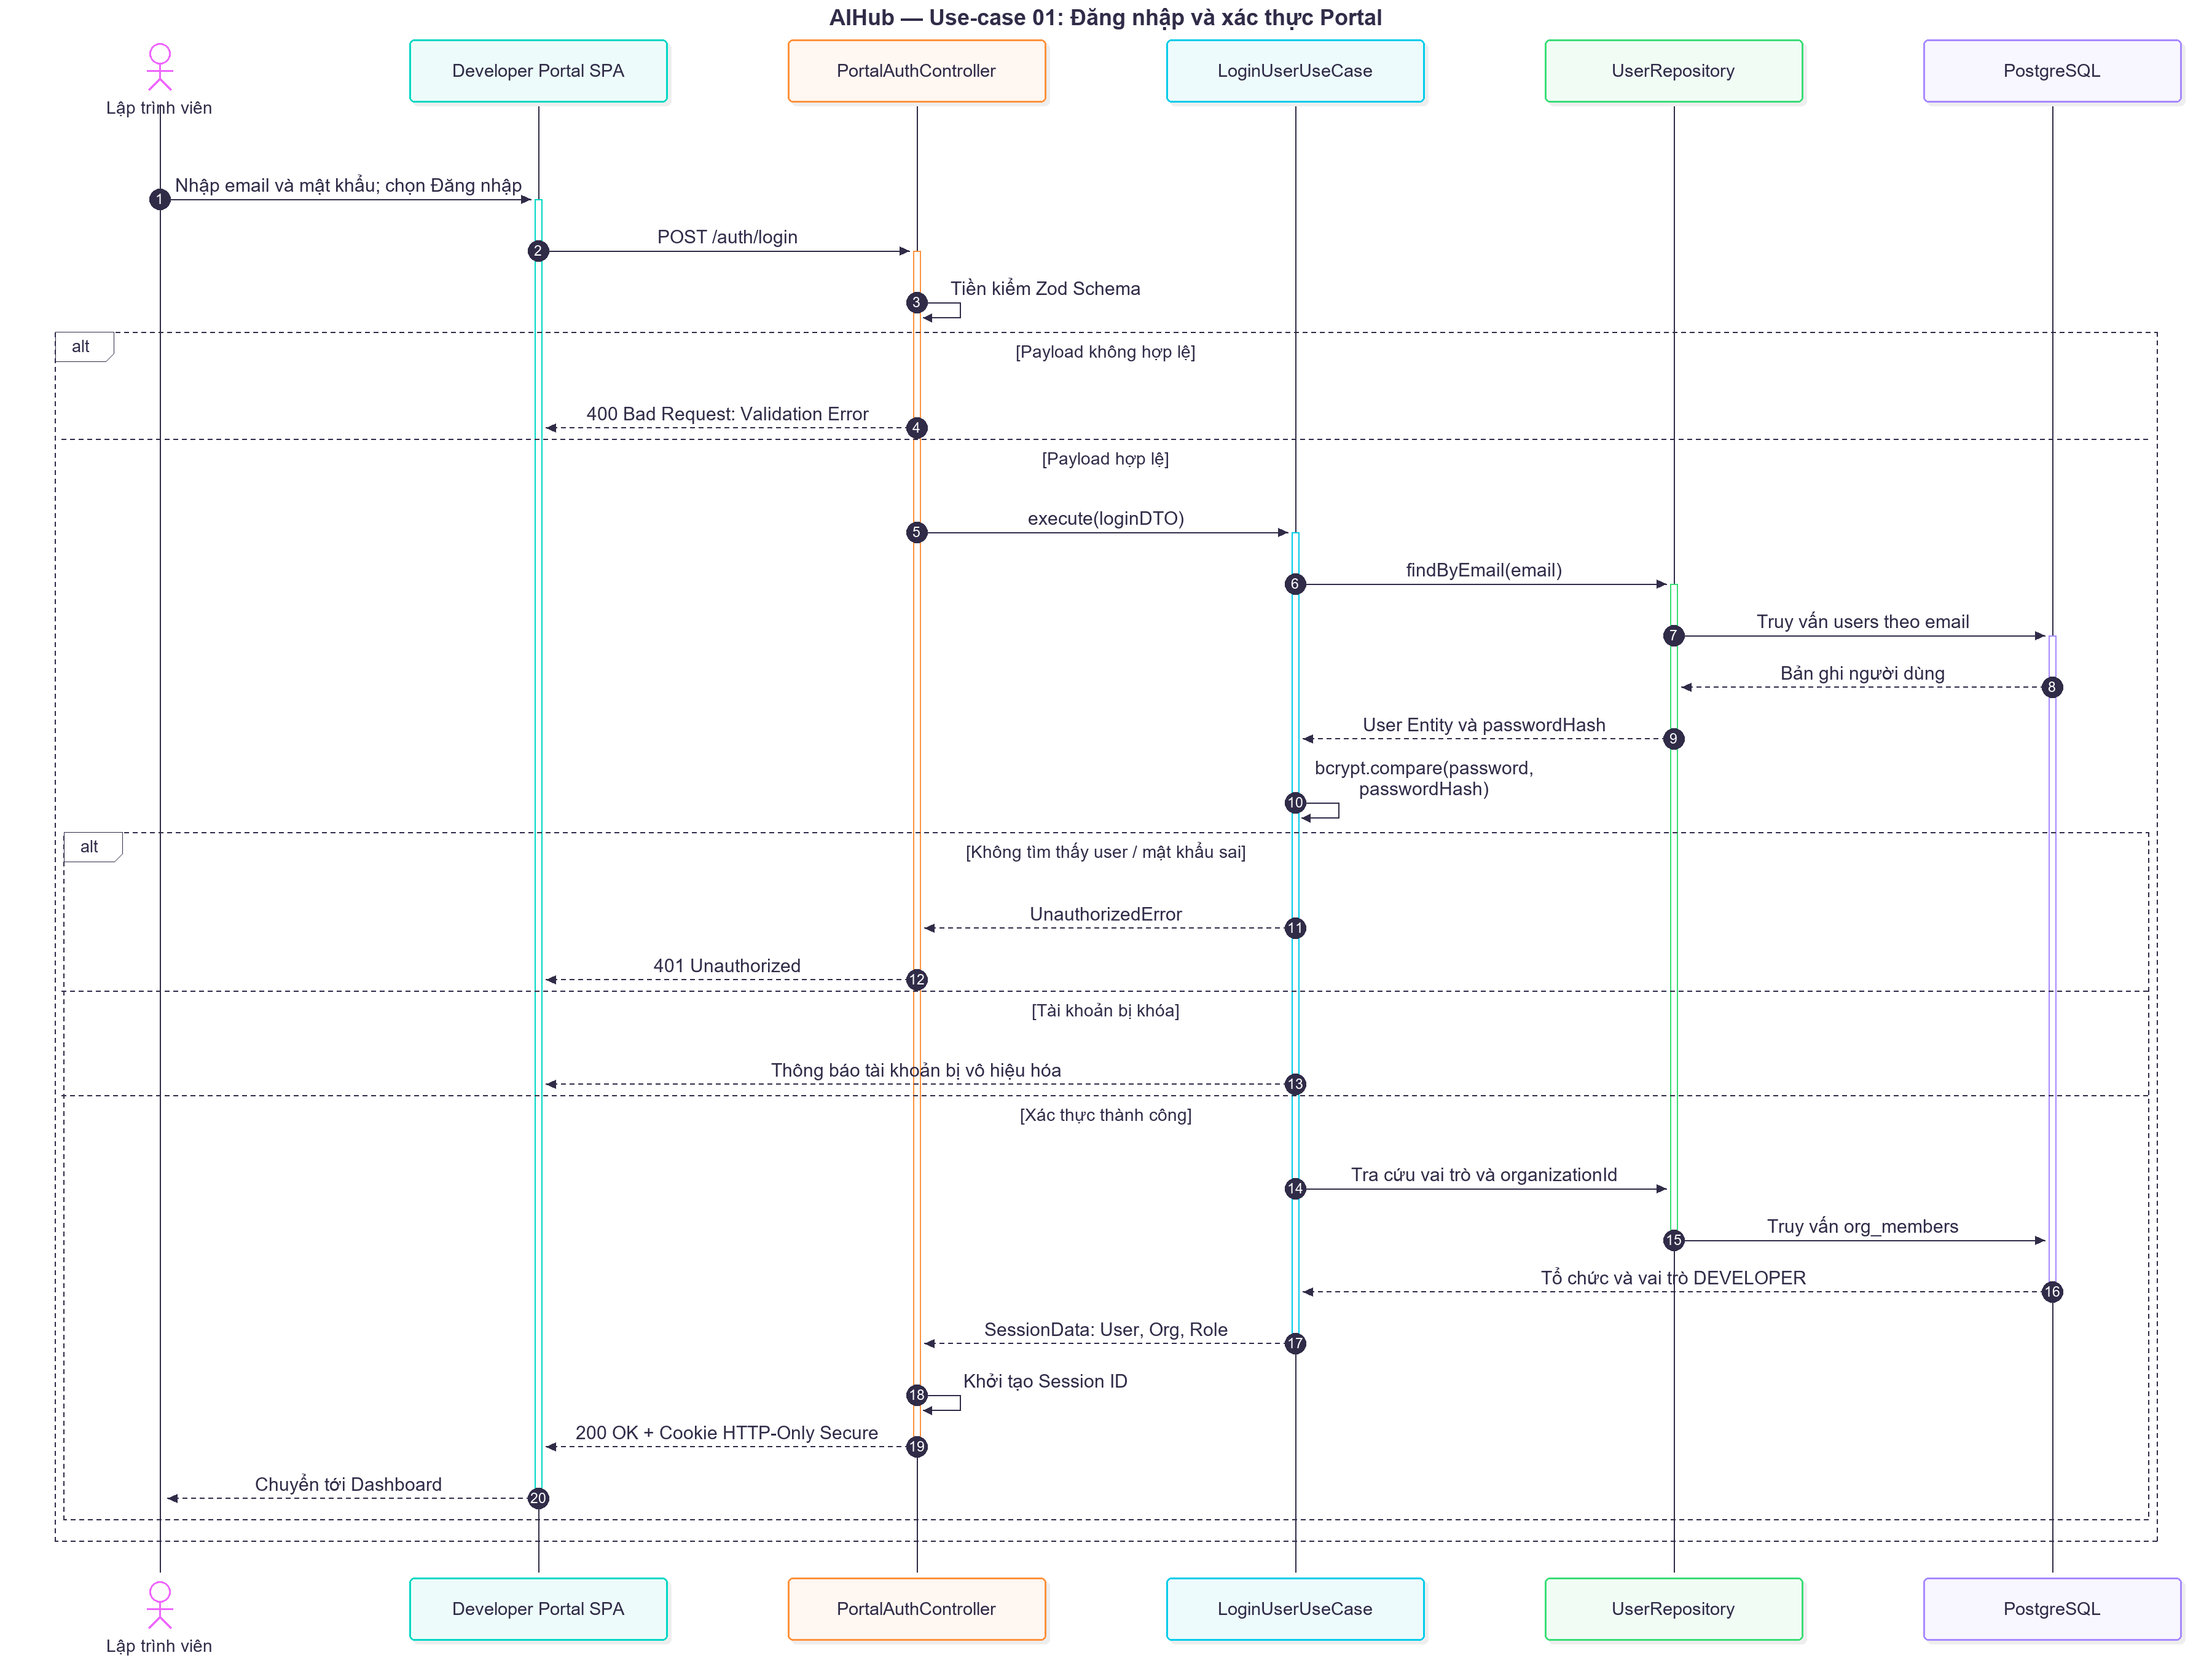
\includegraphics[width=\linewidth,height=.77\textheight,keepaspectratio]{Images/Sequence/AIHub/sequence_uc01_portal_auth.png}
\caption{Sequence diagram AIHub UC01 — Xác thực Developer Portal}
\label{sequence:aihub:sequence_uc01_portal_auth}
\end{figure}

Portal dùng danh tính người dùng; xác thực API đối tác là cơ chế riêng bằng credentials tổ chức.

\clearpage
\paragraph*{UC02. Quản lý khóa API}

\begin{figure}[H]
\centering
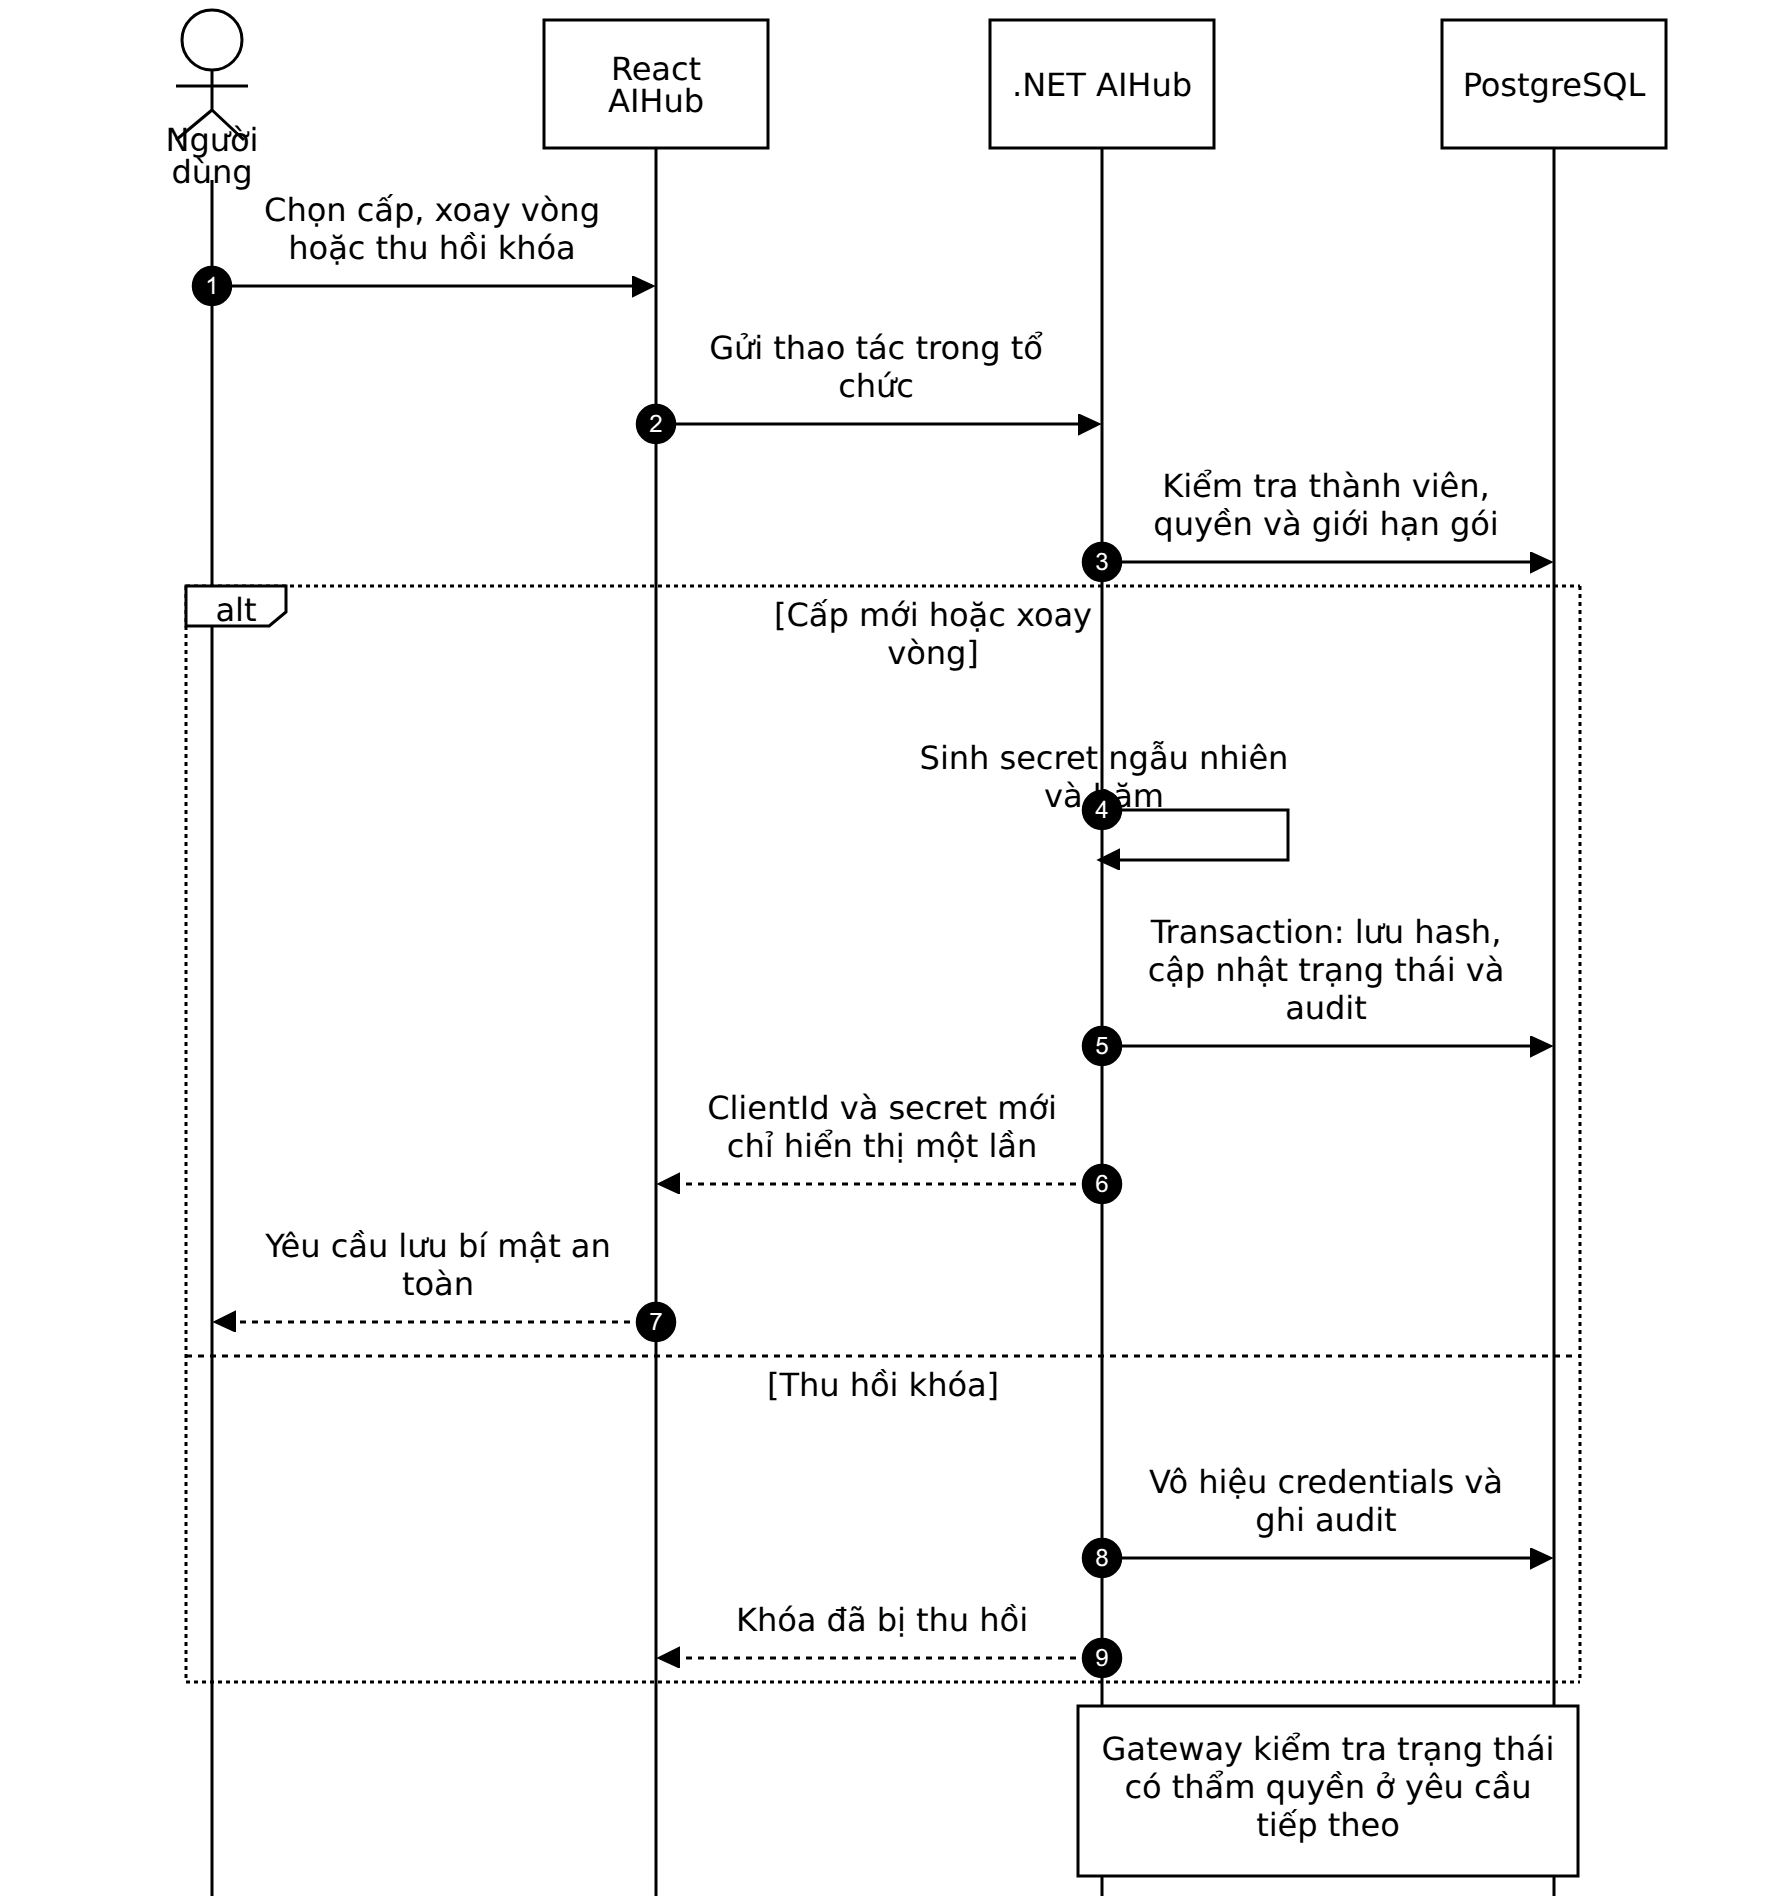
\includegraphics[width=\linewidth,height=.77\textheight,keepaspectratio]{Images/Sequence/AIHub/sequence_uc02_api_credentials.png}
\caption{Sequence diagram AIHub UC02 — Quản lý khóa API}
\label{sequence:aihub:sequence_uc02_api_credentials}
\end{figure}

Secret chỉ được trả một lần; phía máy chủ lưu hash và bảo đảm thu hồi có hiệu lực tại Gateway.

\clearpage
\paragraph*{UC03. Kiểm thử cURL Sandbox}

\begin{figure}[H]
\centering
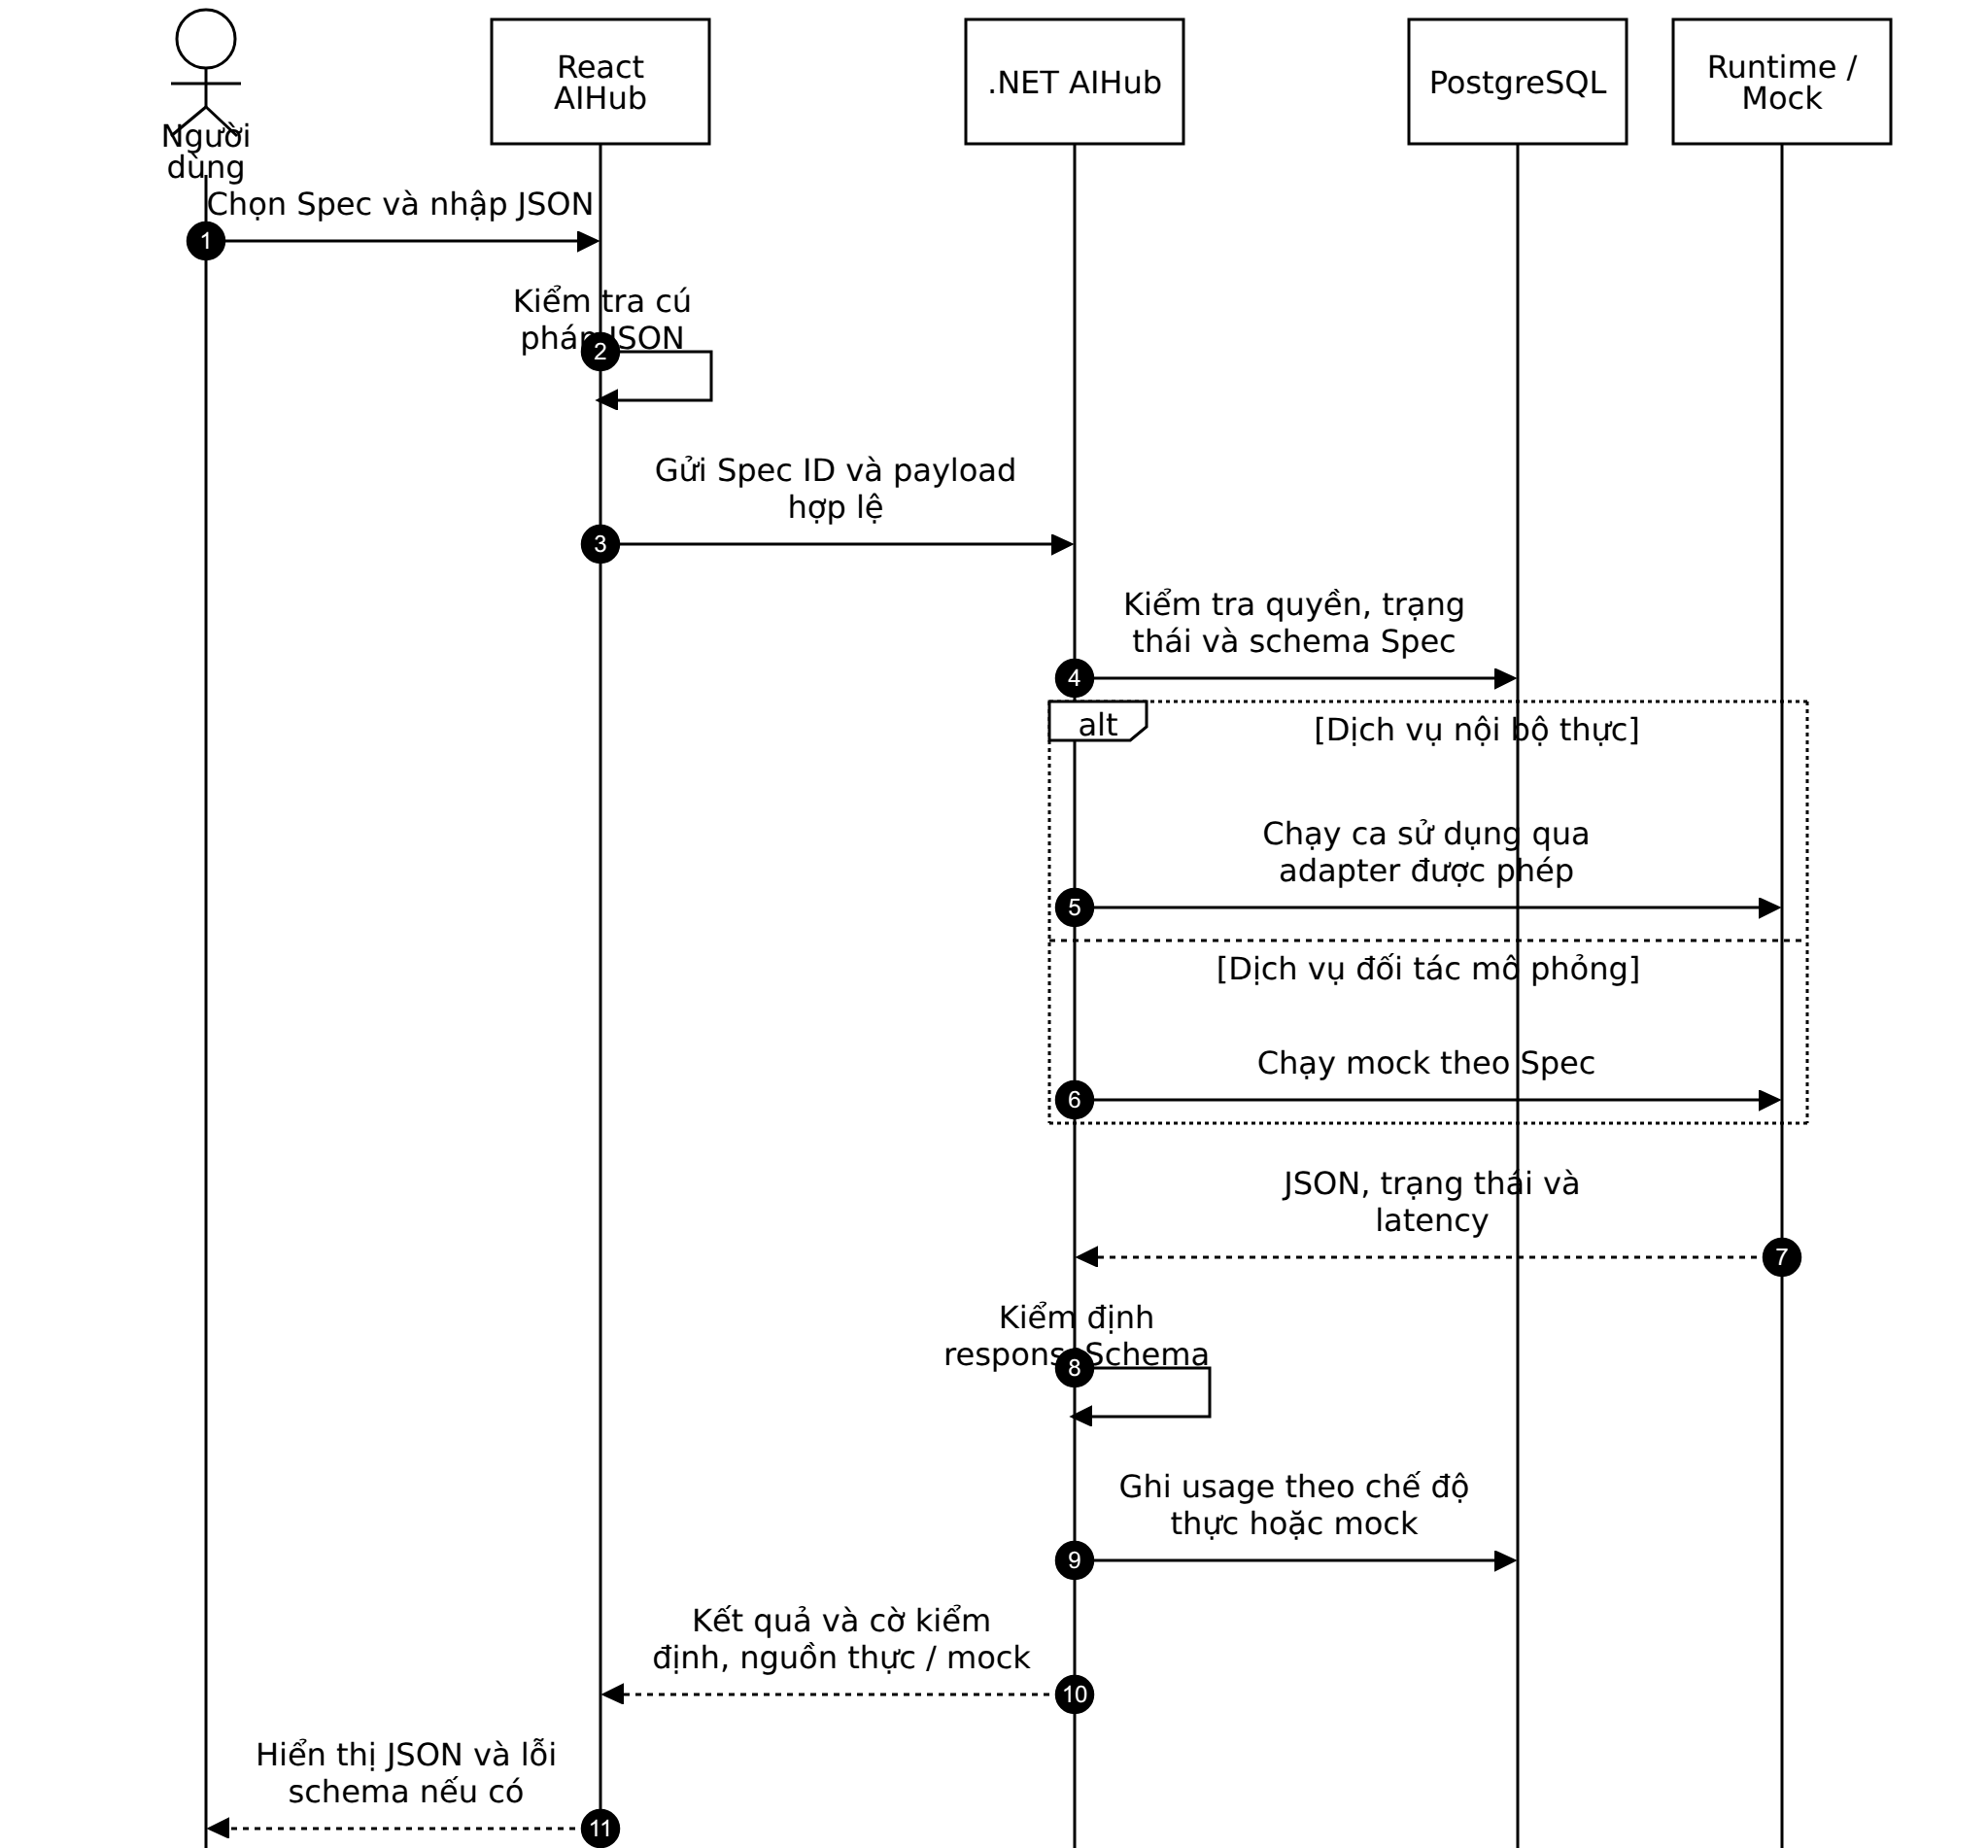
\includegraphics[width=\linewidth,height=.77\textheight,keepaspectratio]{Images/Sequence/AIHub/sequence_uc03_curl_sandbox.png}
\caption{Sequence diagram AIHub UC03 — Kiểm thử cURL Sandbox}
\label{sequence:aihub:sequence_uc03_curl_sandbox}
\end{figure}

Sandbox phân biệt chạy thật với mô phỏng và kiểm định đầu ra theo phiên bản Spec đang hoạt động.

\clearpage
\paragraph*{UC04. Gọi API sinh bài tập vi mô}

\begin{figure}[H]
\centering
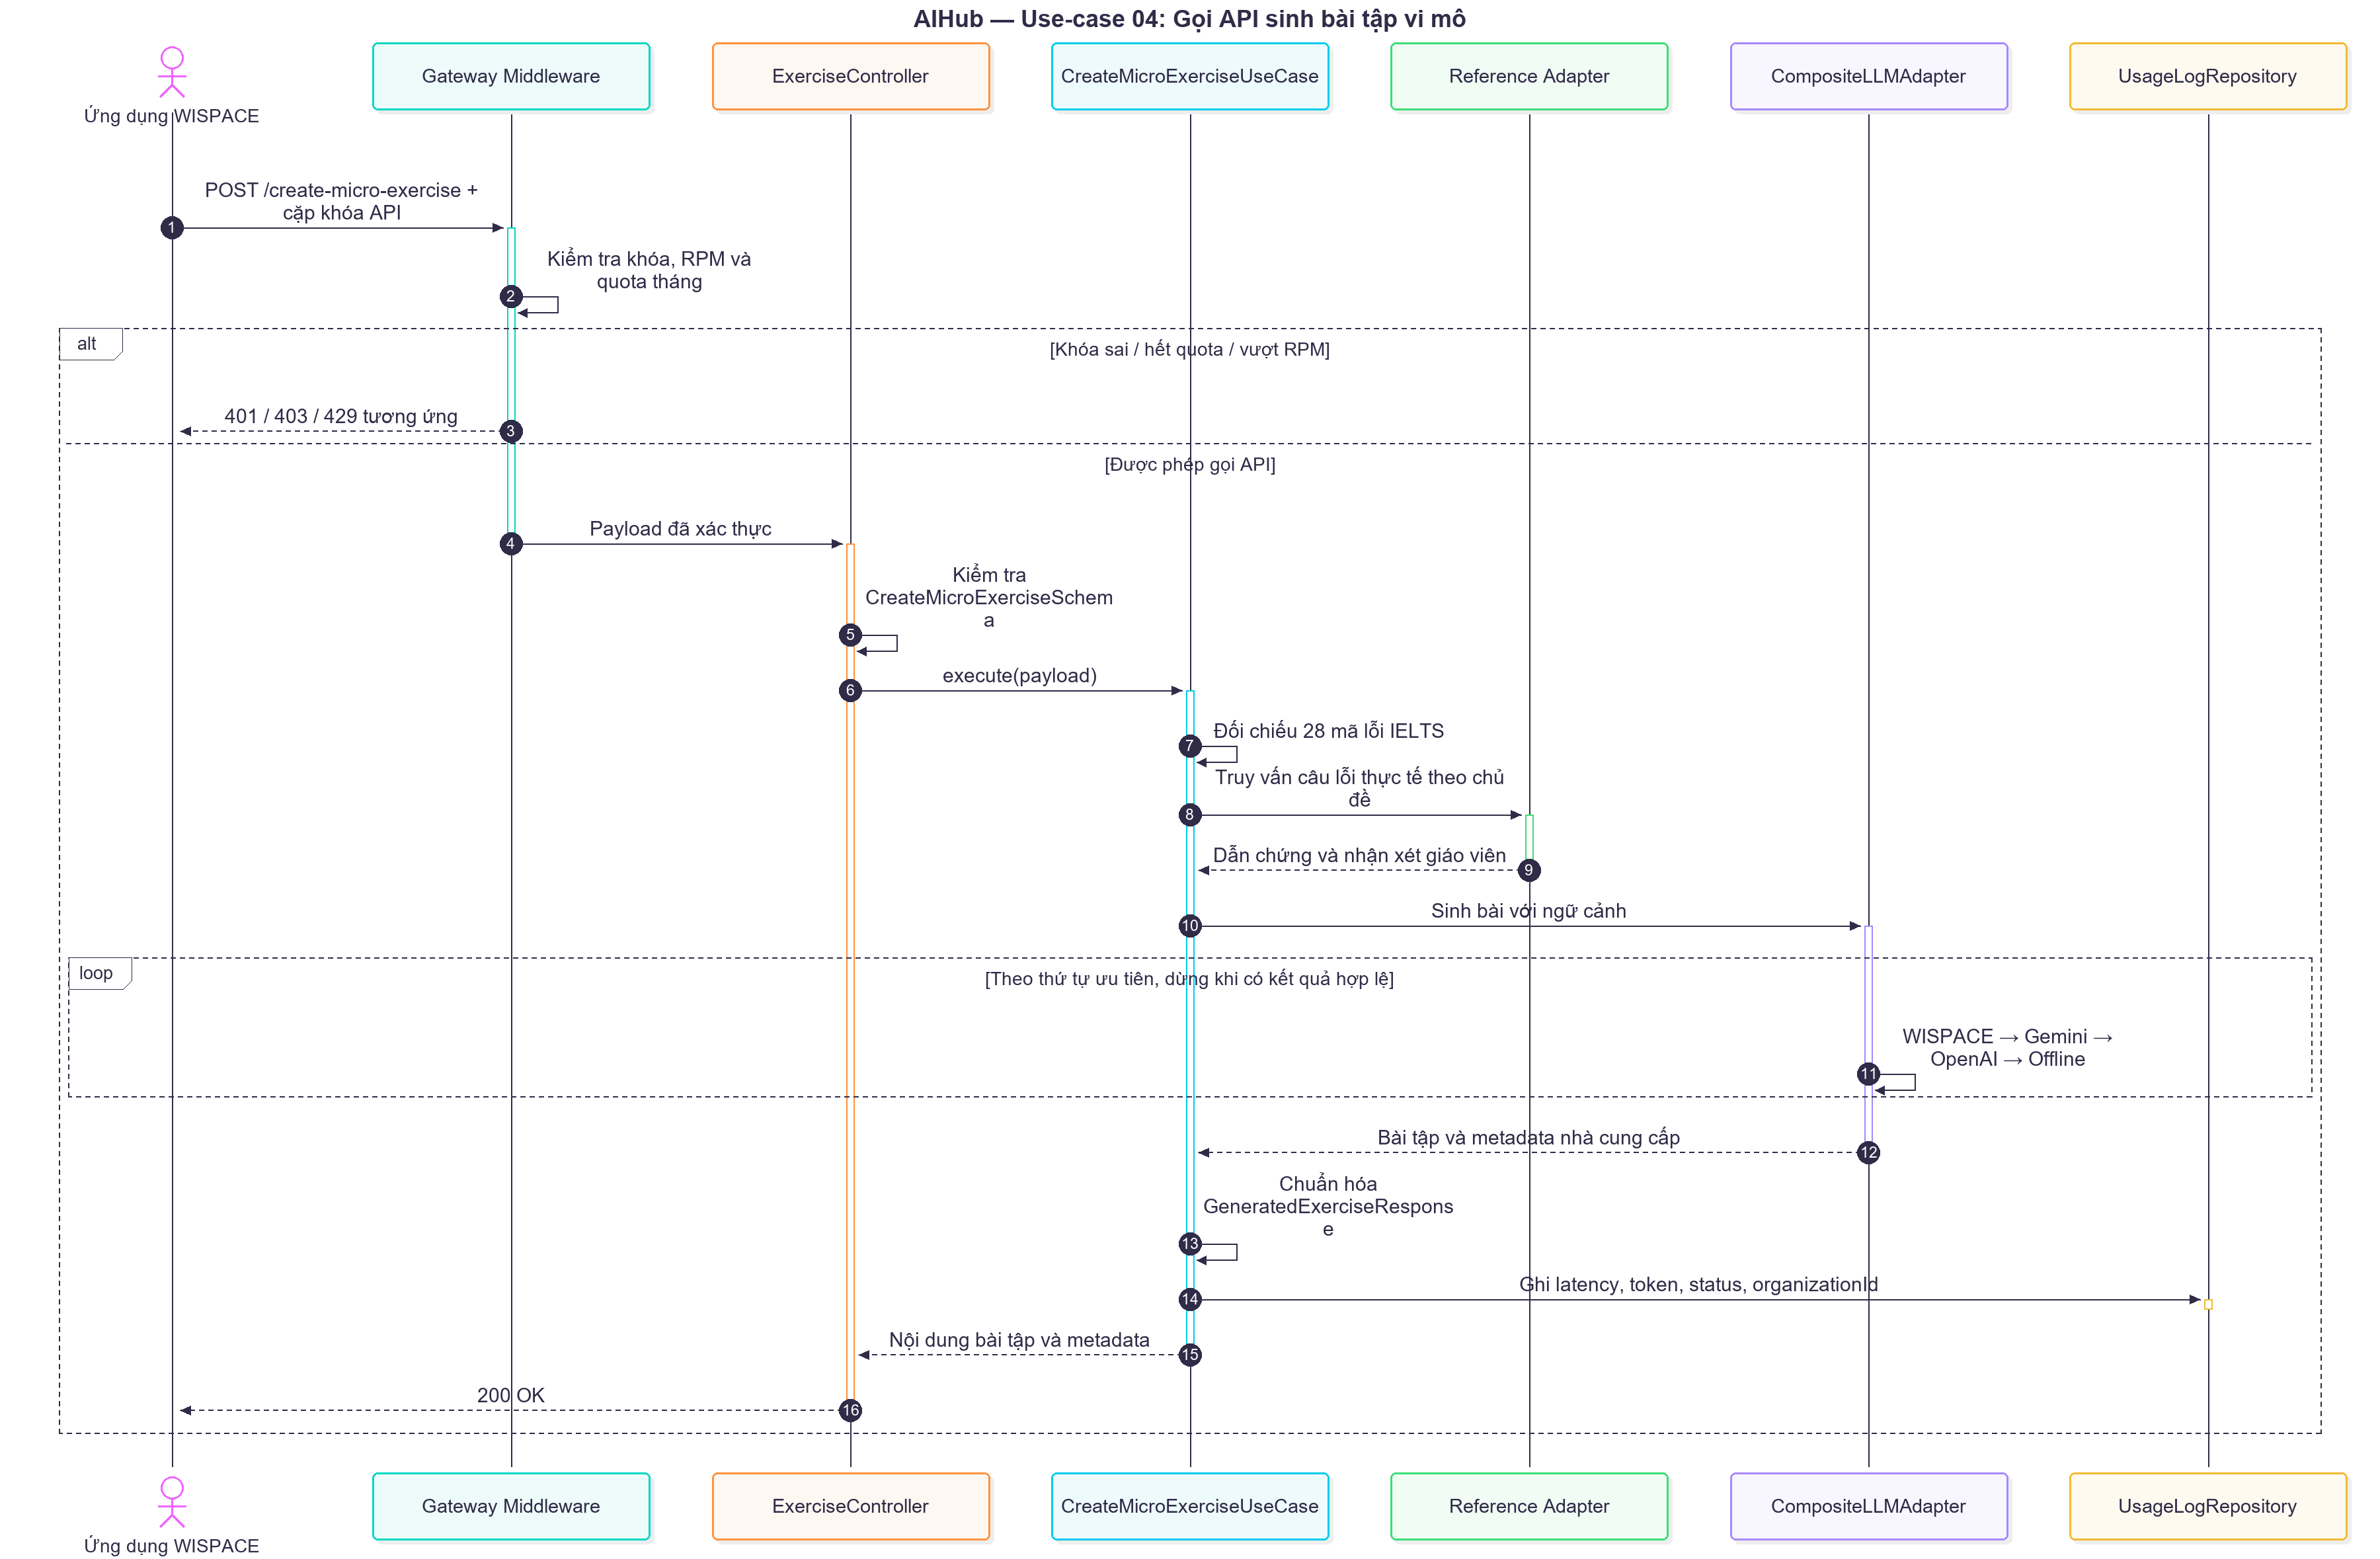
\includegraphics[width=\linewidth,height=.77\textheight,keepaspectratio]{Images/Sequence/AIHub/sequence_uc04_create_micro_exercise.png}
\caption{Sequence diagram AIHub UC04 — Gọi API sinh bài tập vi mô}
\label{sequence:aihub:sequence_uc04_create_micro_exercise}
\end{figure}

Gateway quản lý quyền và hạn mức B2B; adapter xử lý fallback rồi trả kết quả đã được kiểm định.

\clearpage
\paragraph*{UC05. Tra cứu hạn mức và nhật ký}

\begin{figure}[H]
\centering
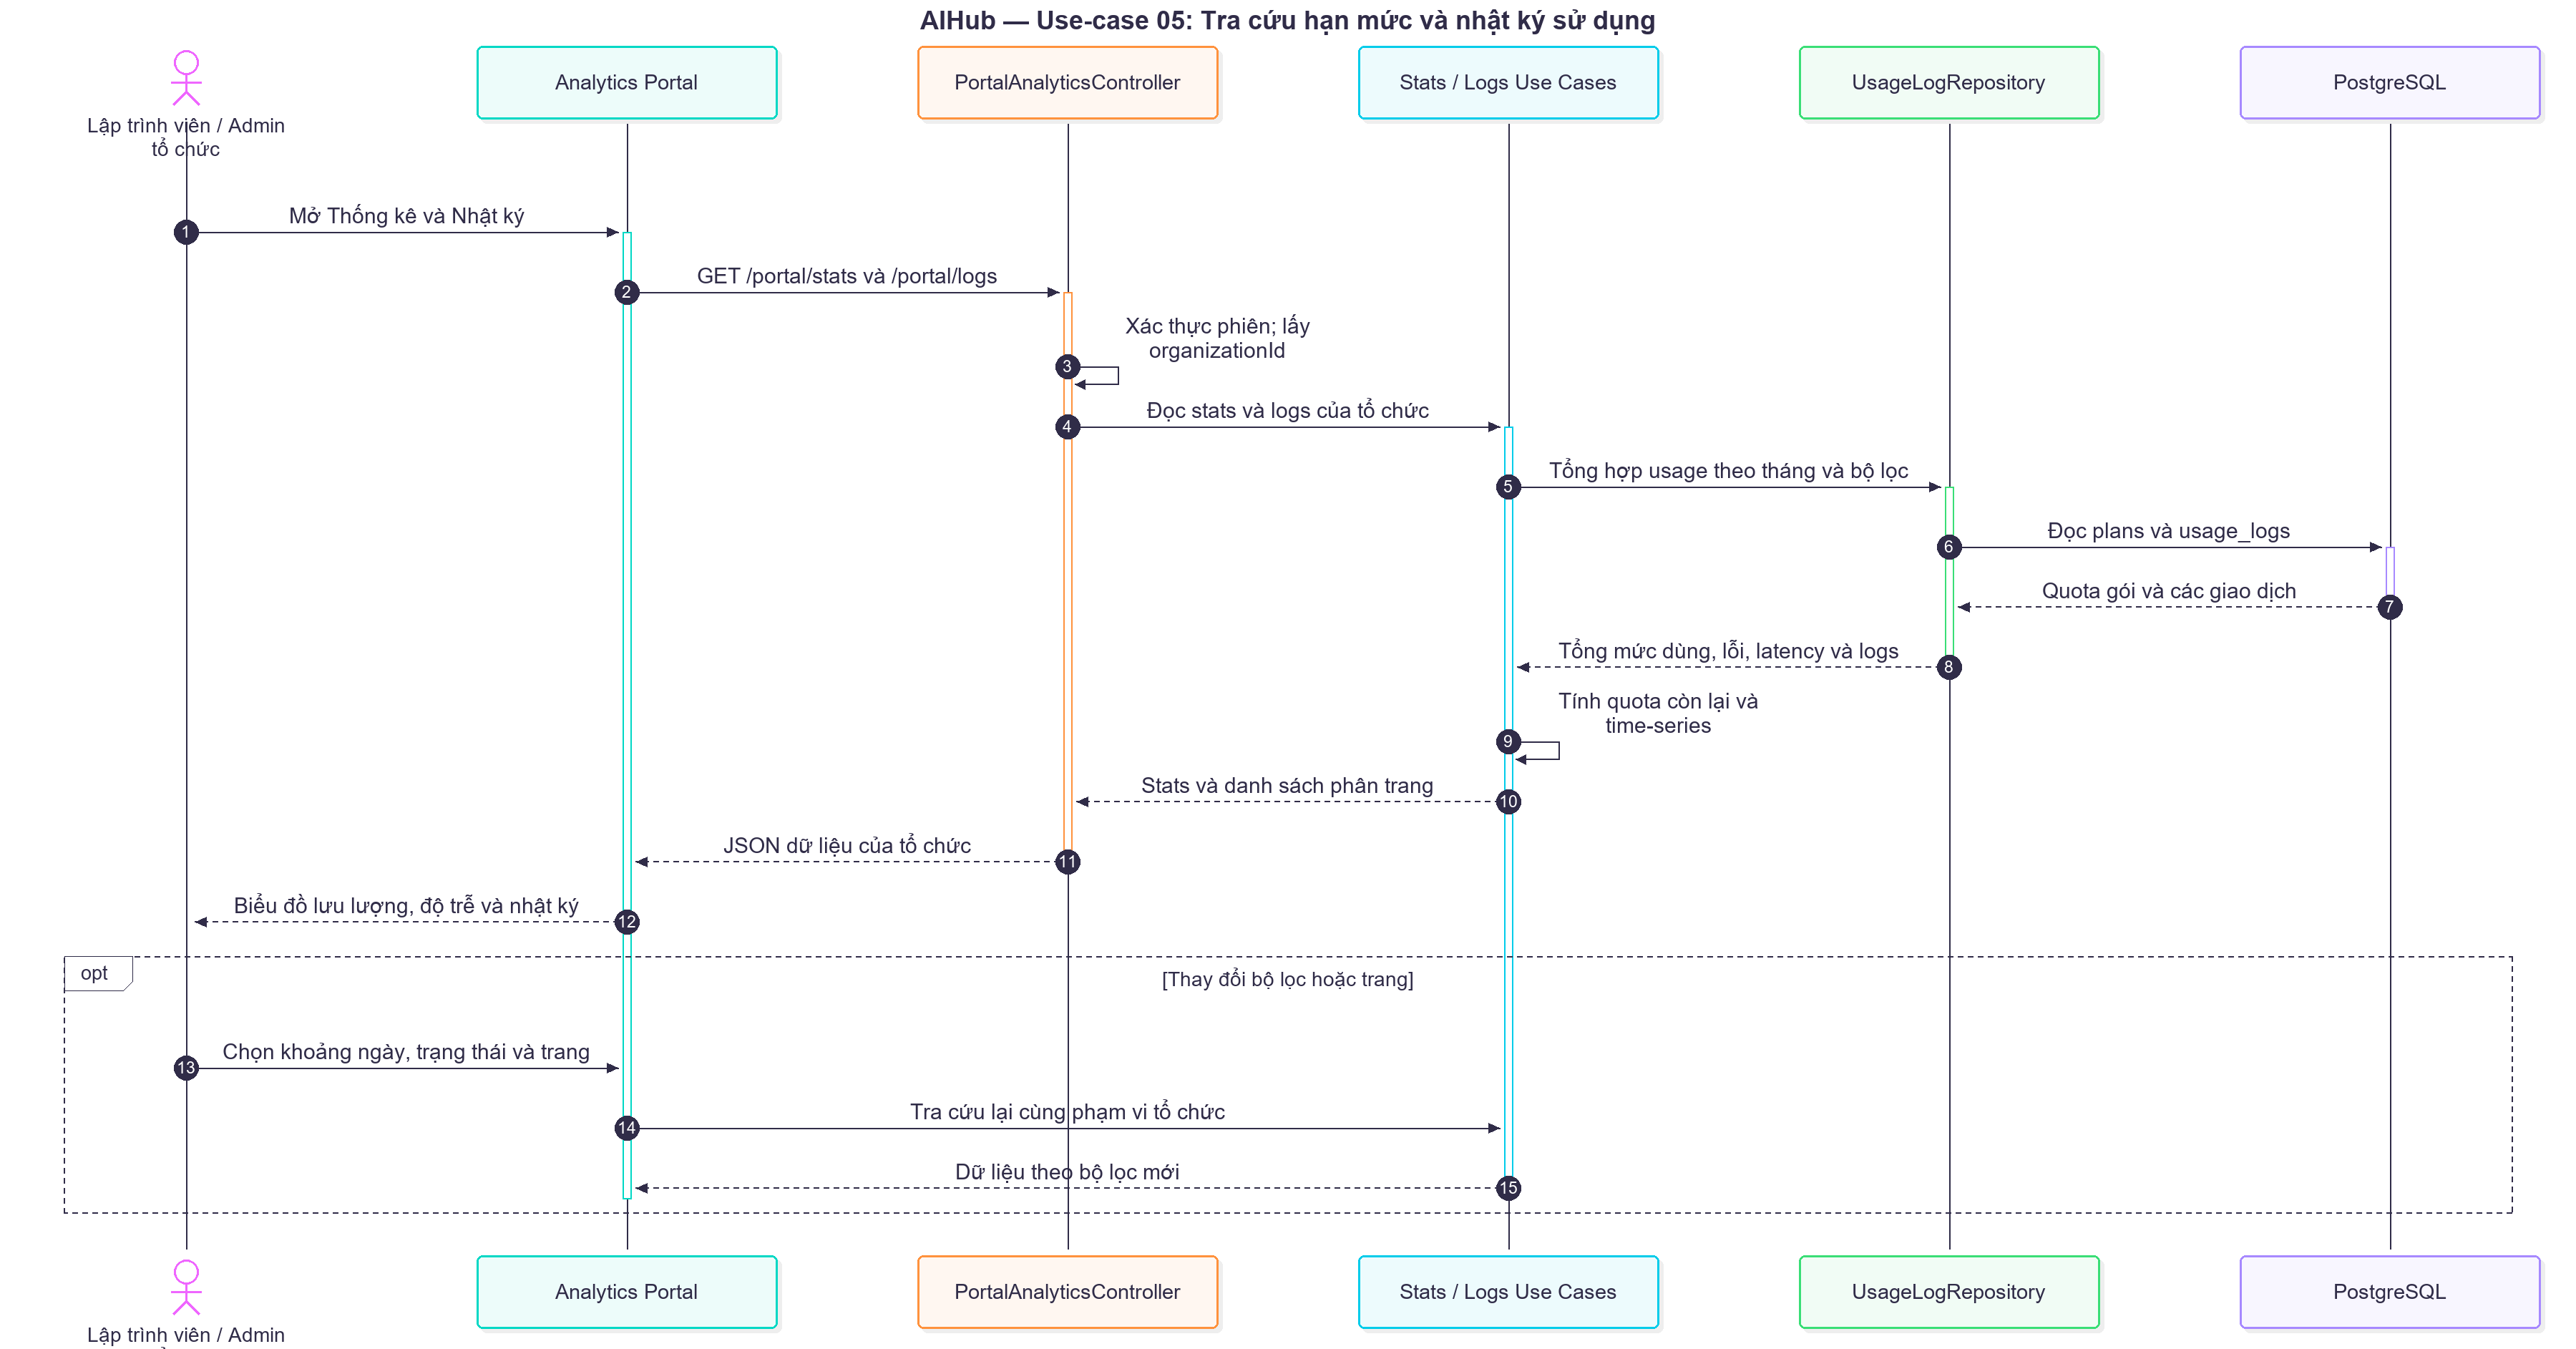
\includegraphics[width=\linewidth,height=.77\textheight,keepaspectratio]{Images/Sequence/AIHub/sequence_uc05_quota_usage_logs.png}
\caption{Sequence diagram AIHub UC05 — Tra cứu hạn mức và nhật ký}
\label{sequence:aihub:sequence_uc05_quota_usage_logs}
\end{figure}

Cả thống kê lẫn nhật ký được giới hạn theo tổ chức; các chi phí mô hình được tách khỏi hạn mức nghiệp vụ.

\clearpage
\paragraph*{UC06. Tra cứu dẫn chứng học thuật}

\begin{figure}[H]
\centering
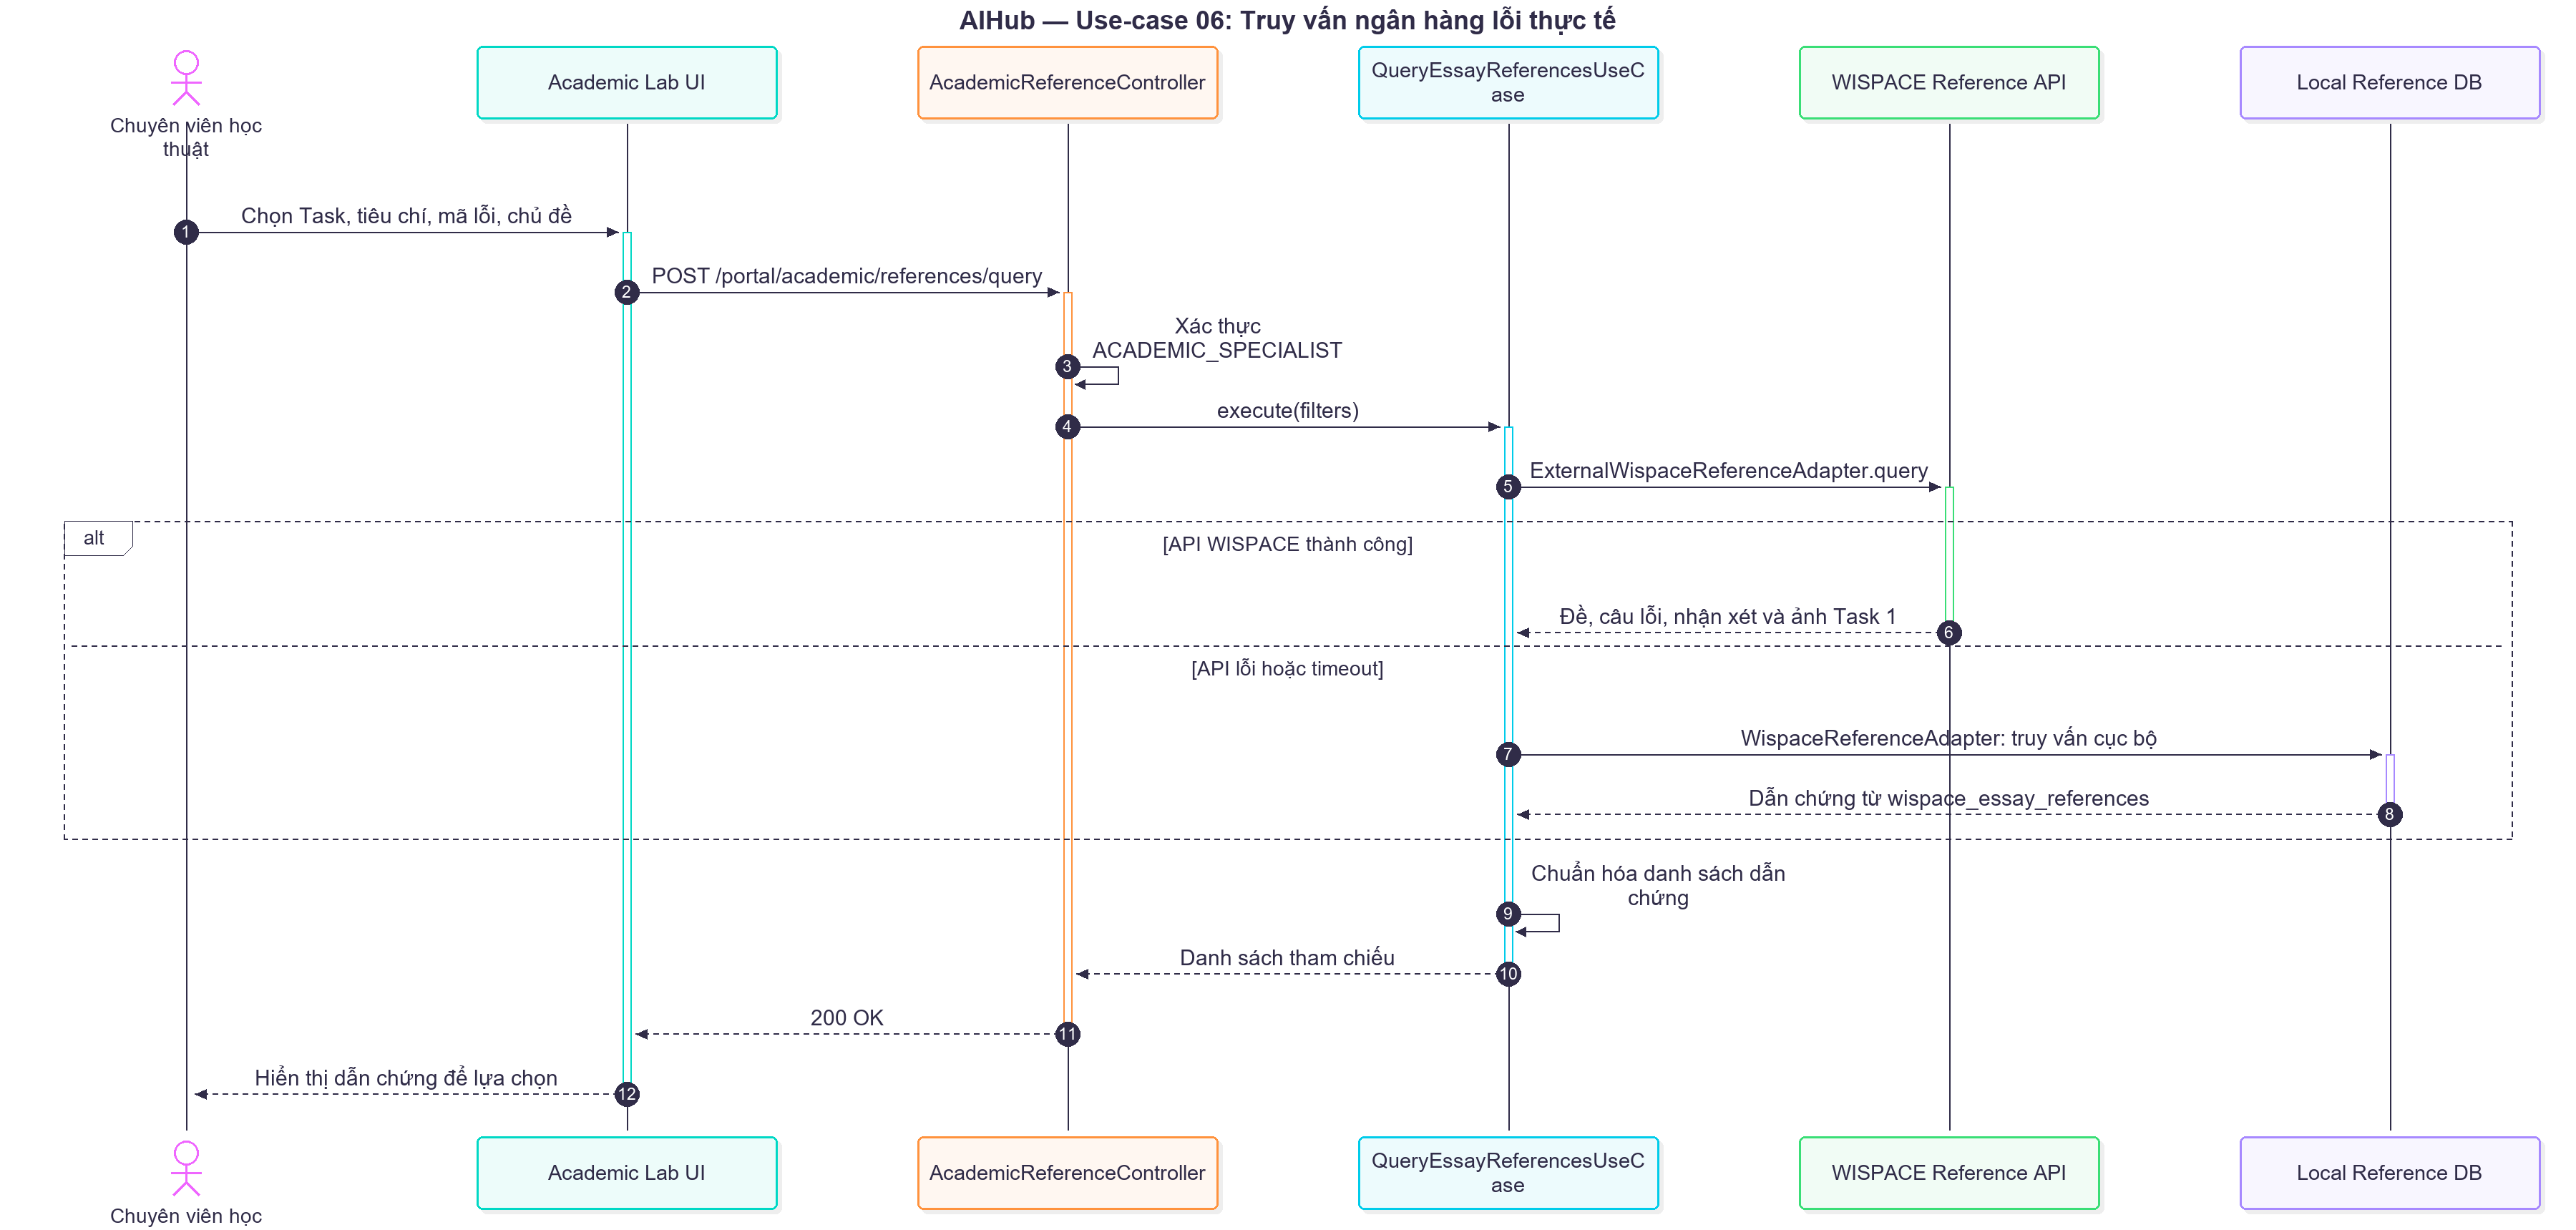
\includegraphics[width=\linewidth,height=.77\textheight,keepaspectratio]{Images/Sequence/AIHub/sequence_uc06_essay_references.png}
\caption{Sequence diagram AIHub UC06 — Tra cứu dẫn chứng học thuật}
\label{sequence:aihub:sequence_uc06_essay_references}
\end{figure}

Lỗi kết nối mới kích hoạt nguồn cục bộ; kết quả rỗng vẫn là kết quả nghiệp vụ hợp lệ.

\clearpage
\paragraph*{UC07. Sinh mẫu học thuật}

\begin{figure}[H]
\centering
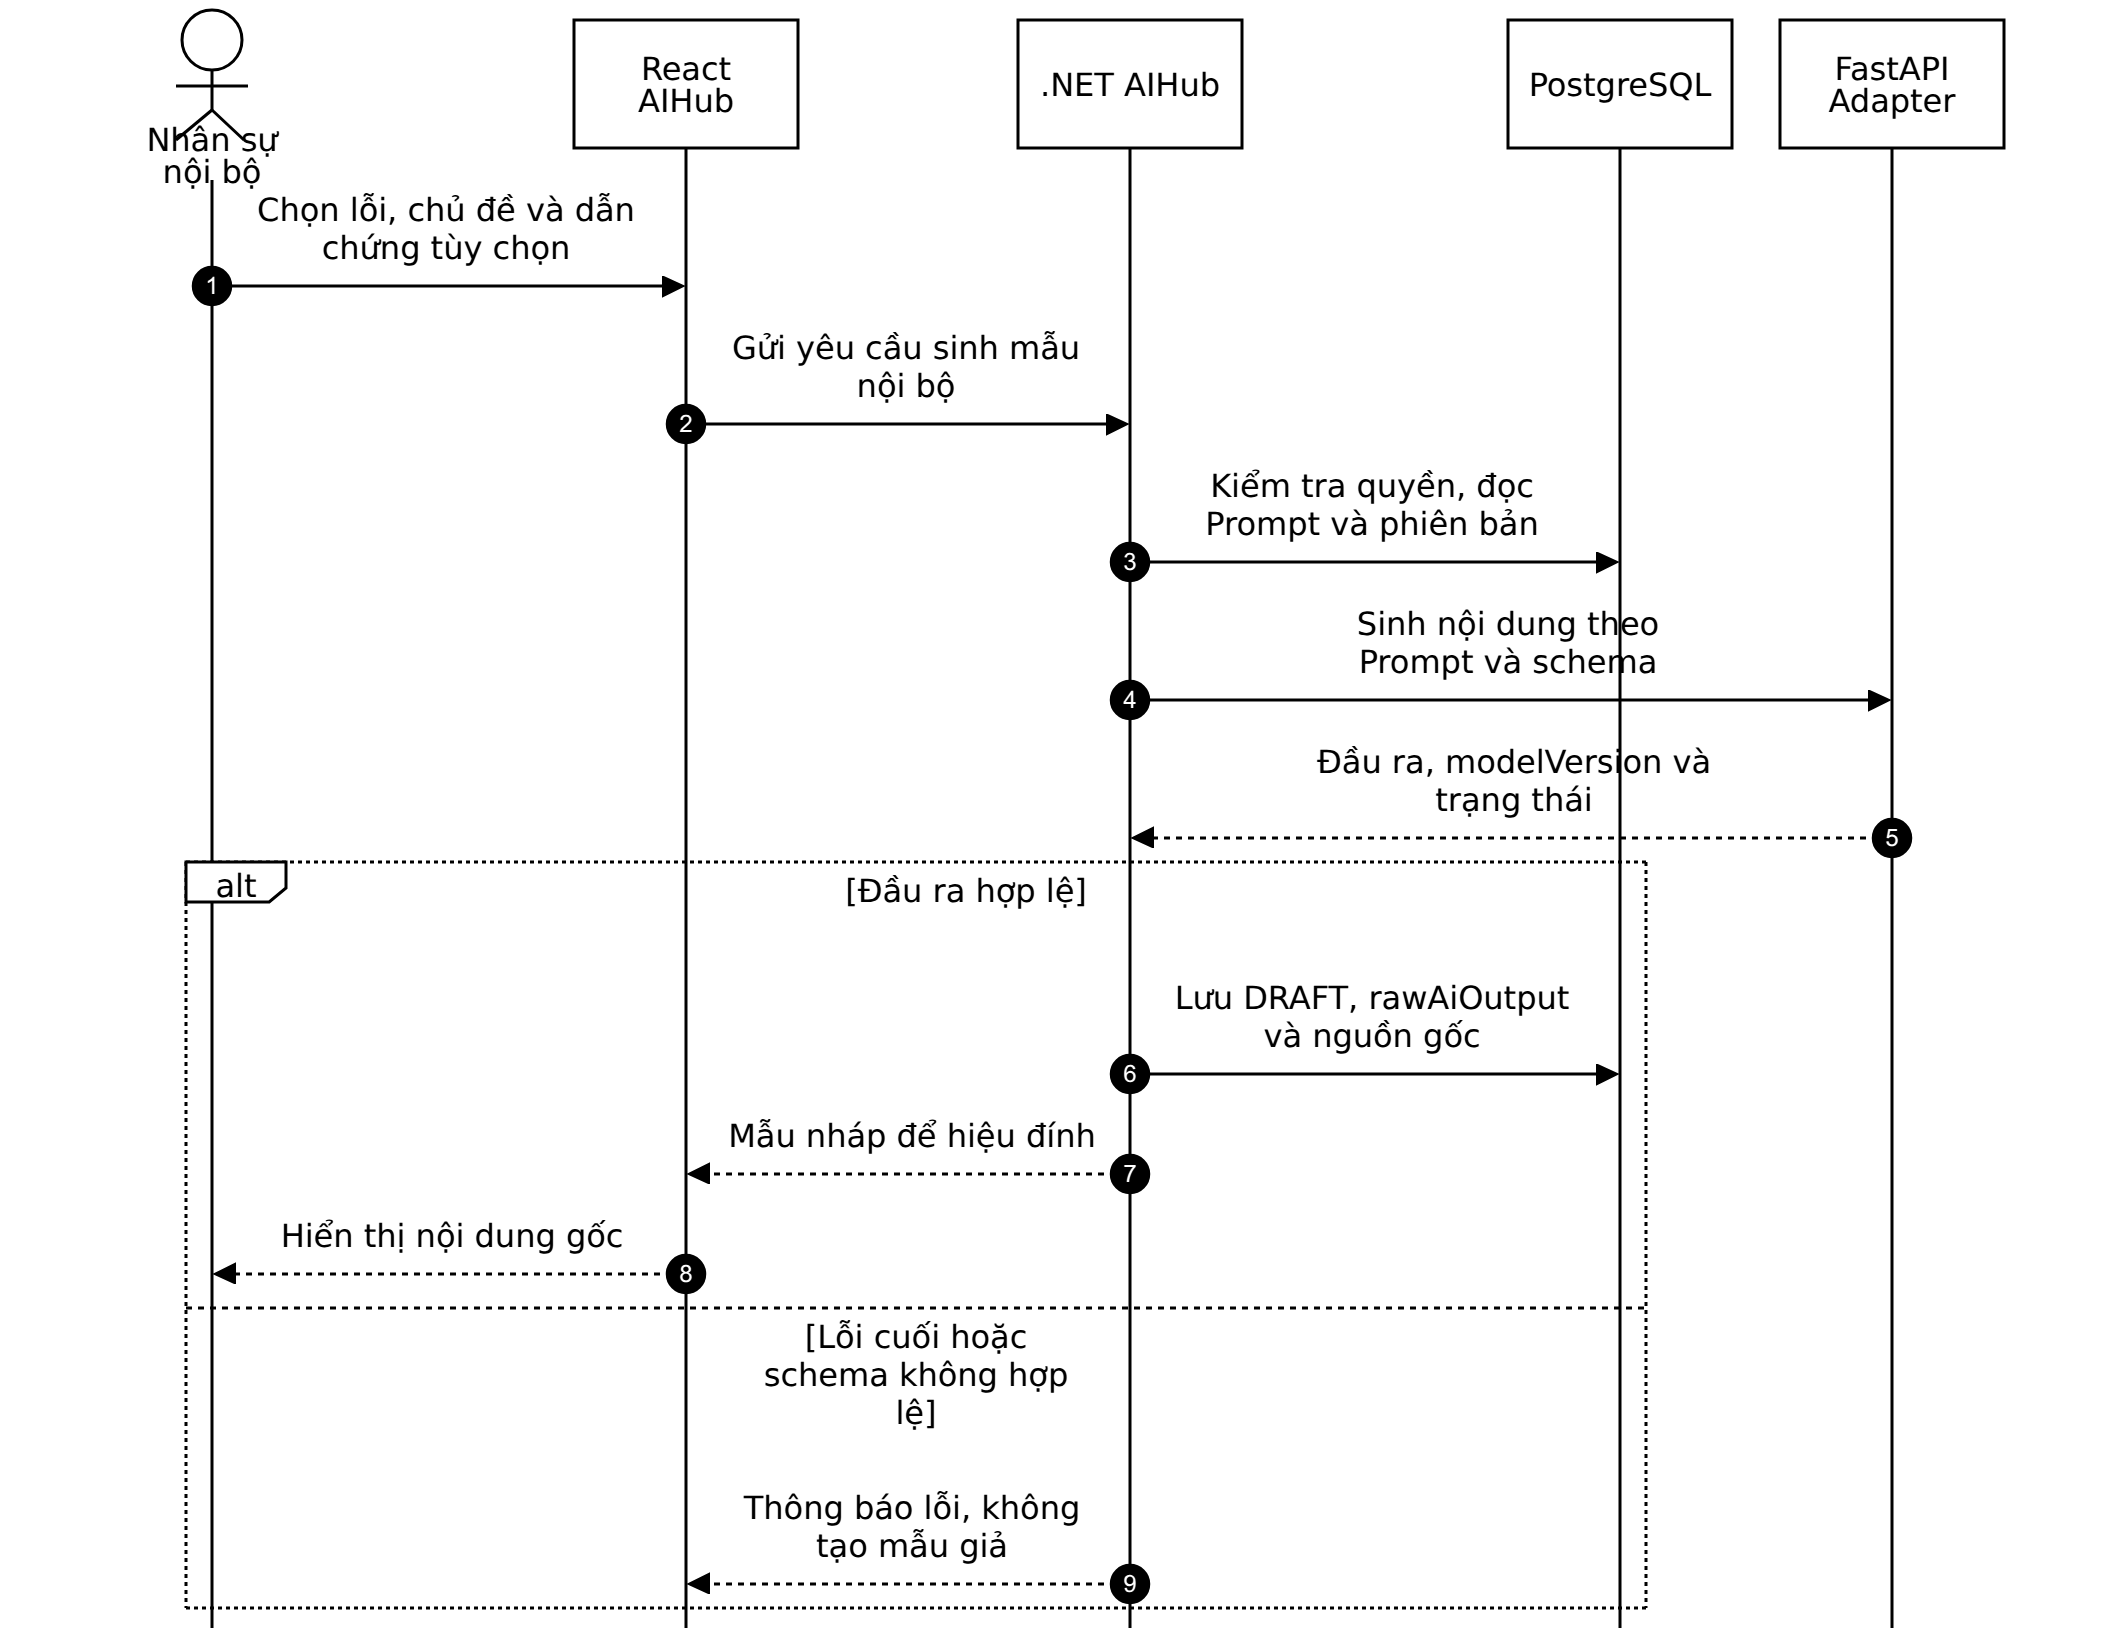
\includegraphics[width=\linewidth,height=.77\textheight,keepaspectratio]{Images/Sequence/AIHub/sequence_uc07_generate_academic_sample.png}
\caption{Sequence diagram AIHub UC07 — Sinh mẫu học thuật}
\label{sequence:aihub:sequence_uc07_generate_academic_sample}
\end{figure}

Chỉ tạo DRAFT khi đã có đầu ra hợp lệ; lưu Prompt và phiên bản mô hình để truy vết.

\clearpage
\paragraph*{UC08. Hiệu đính và chấm điểm mẫu}

\begin{figure}[H]
\centering
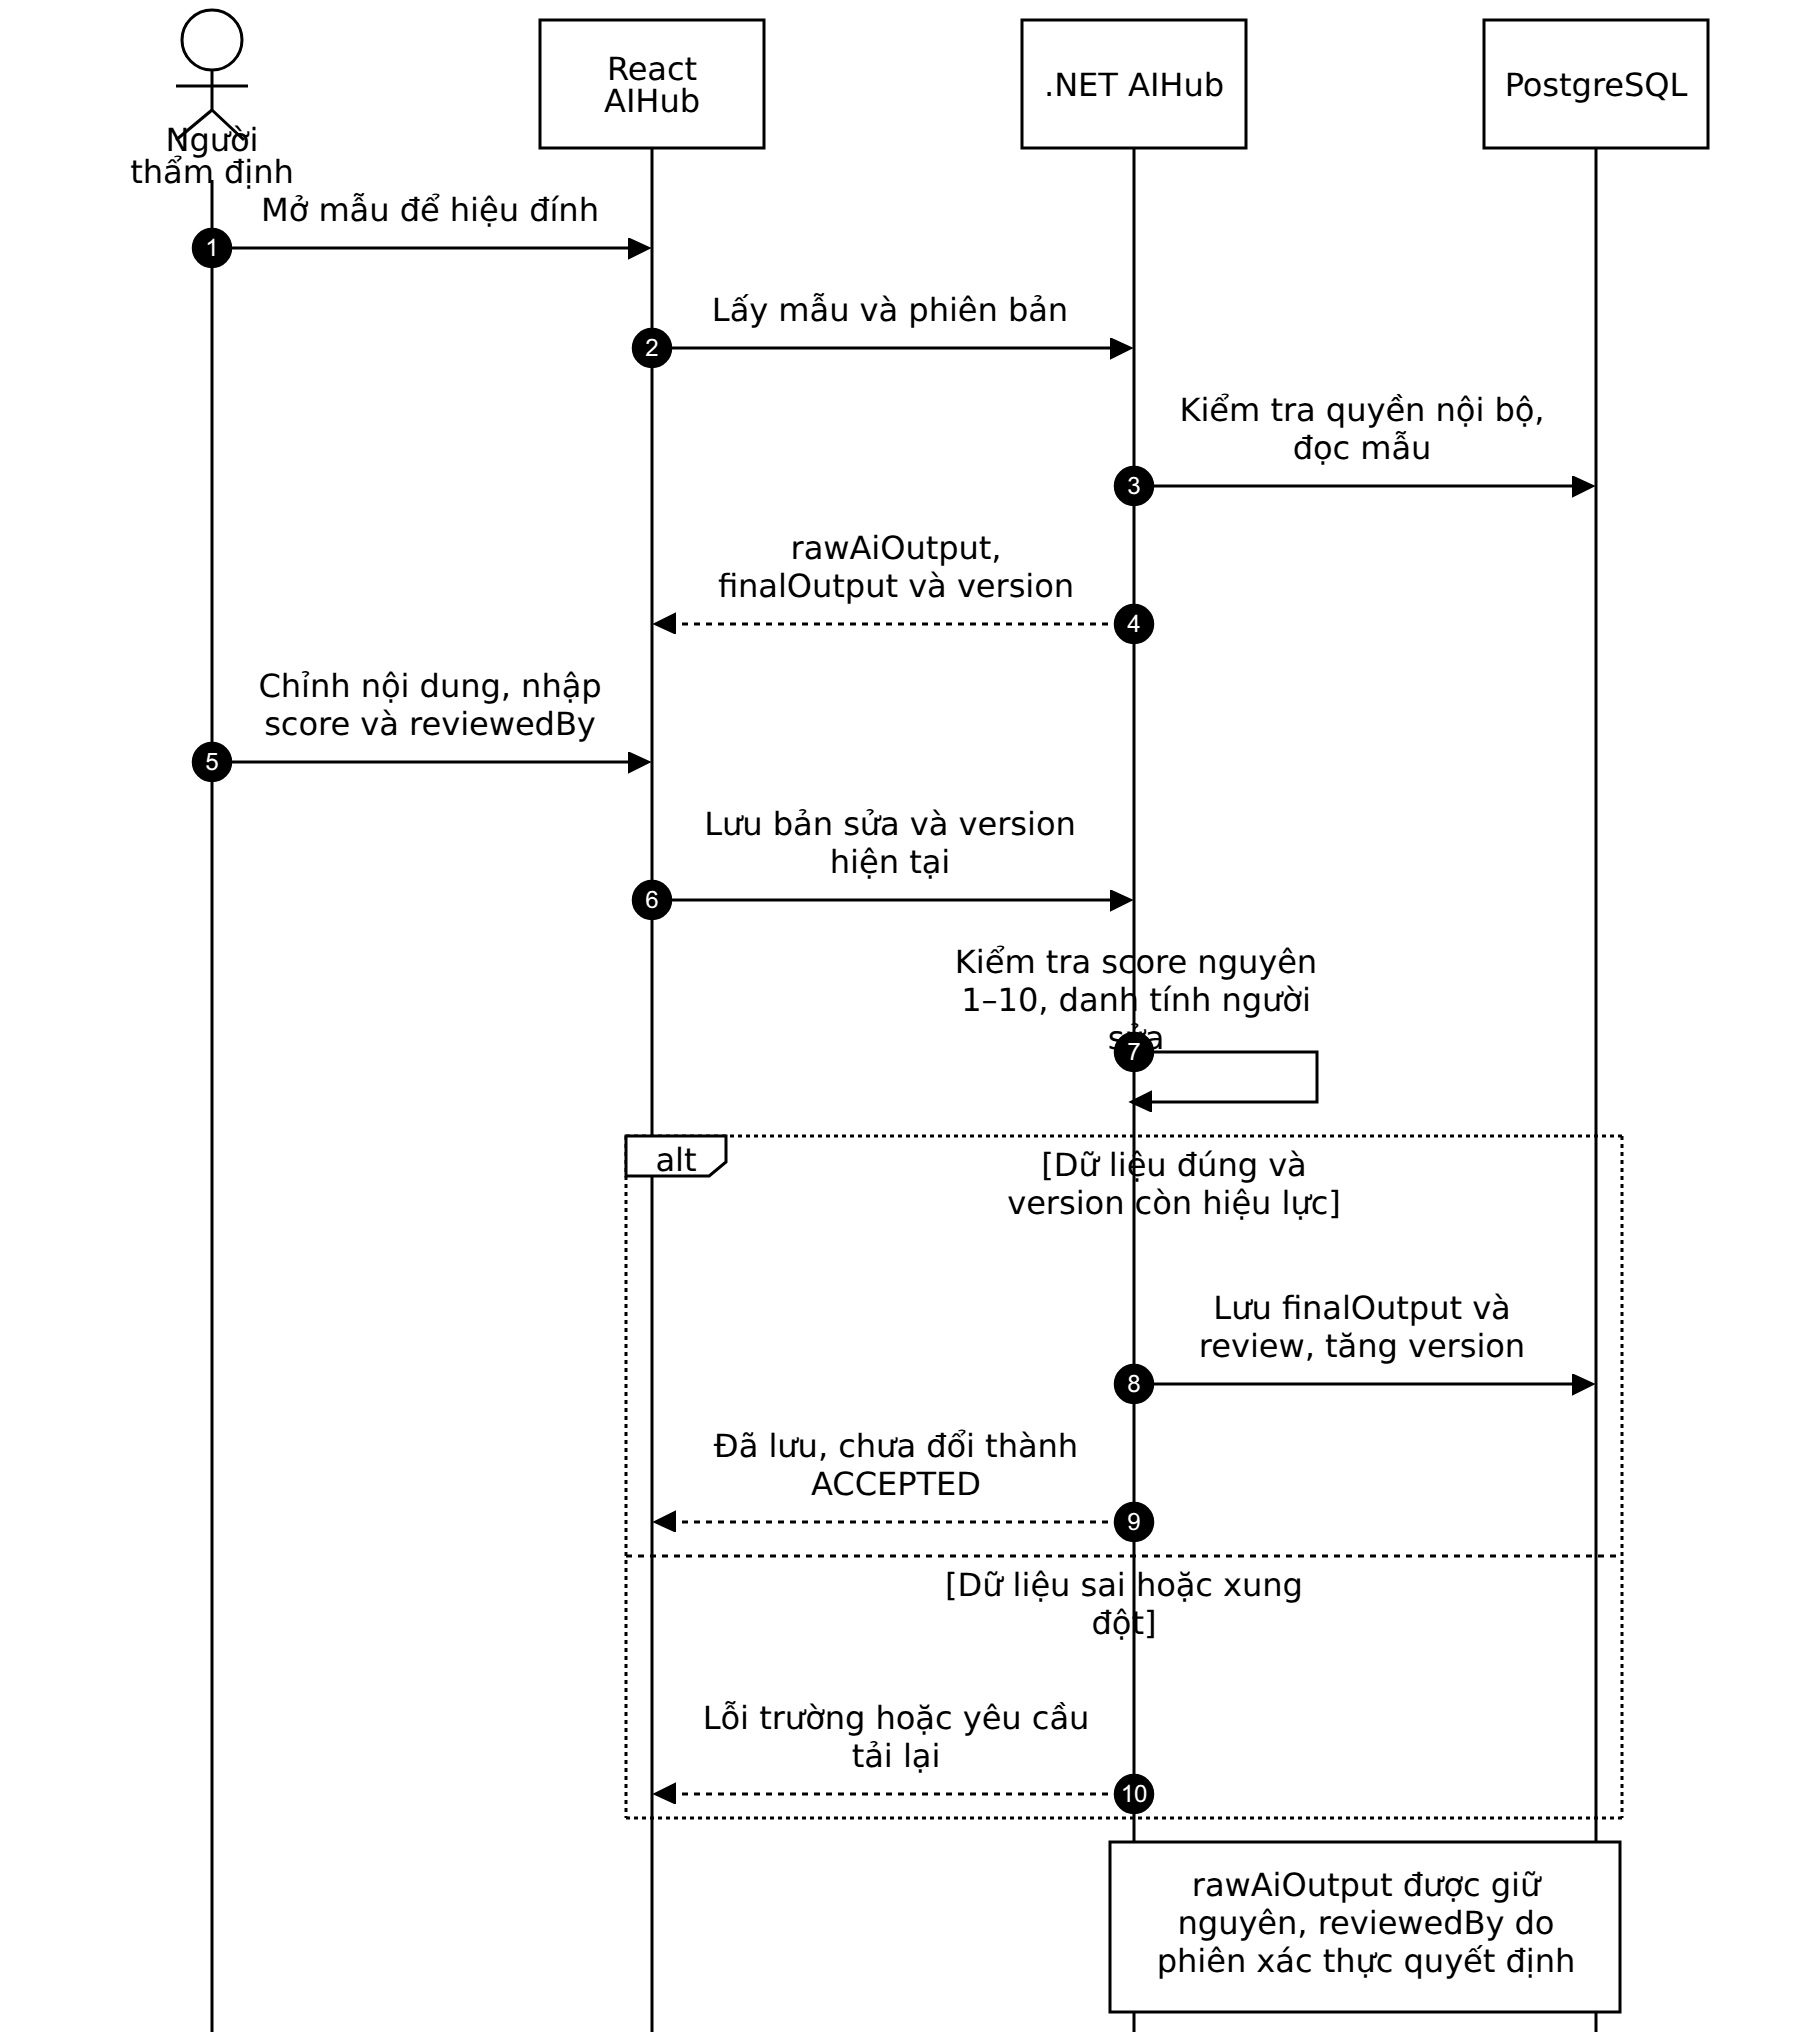
\includegraphics[width=\linewidth,height=.77\textheight,keepaspectratio]{Images/Sequence/AIHub/sequence_uc08_review_score_sample.png}
\caption{Sequence diagram AIHub UC08 — Hiệu đính và chấm điểm mẫu}
\label{sequence:aihub:sequence_uc08_review_score_sample}
\end{figure}

Lưu bản sửa không tự chấp thuận mẫu; kiểm tra phiên bản và danh tính người thẩm định trên máy chủ.

\clearpage
\paragraph*{UC09. Chấp thuận mẫu học thuật}

\begin{figure}[H]
\centering
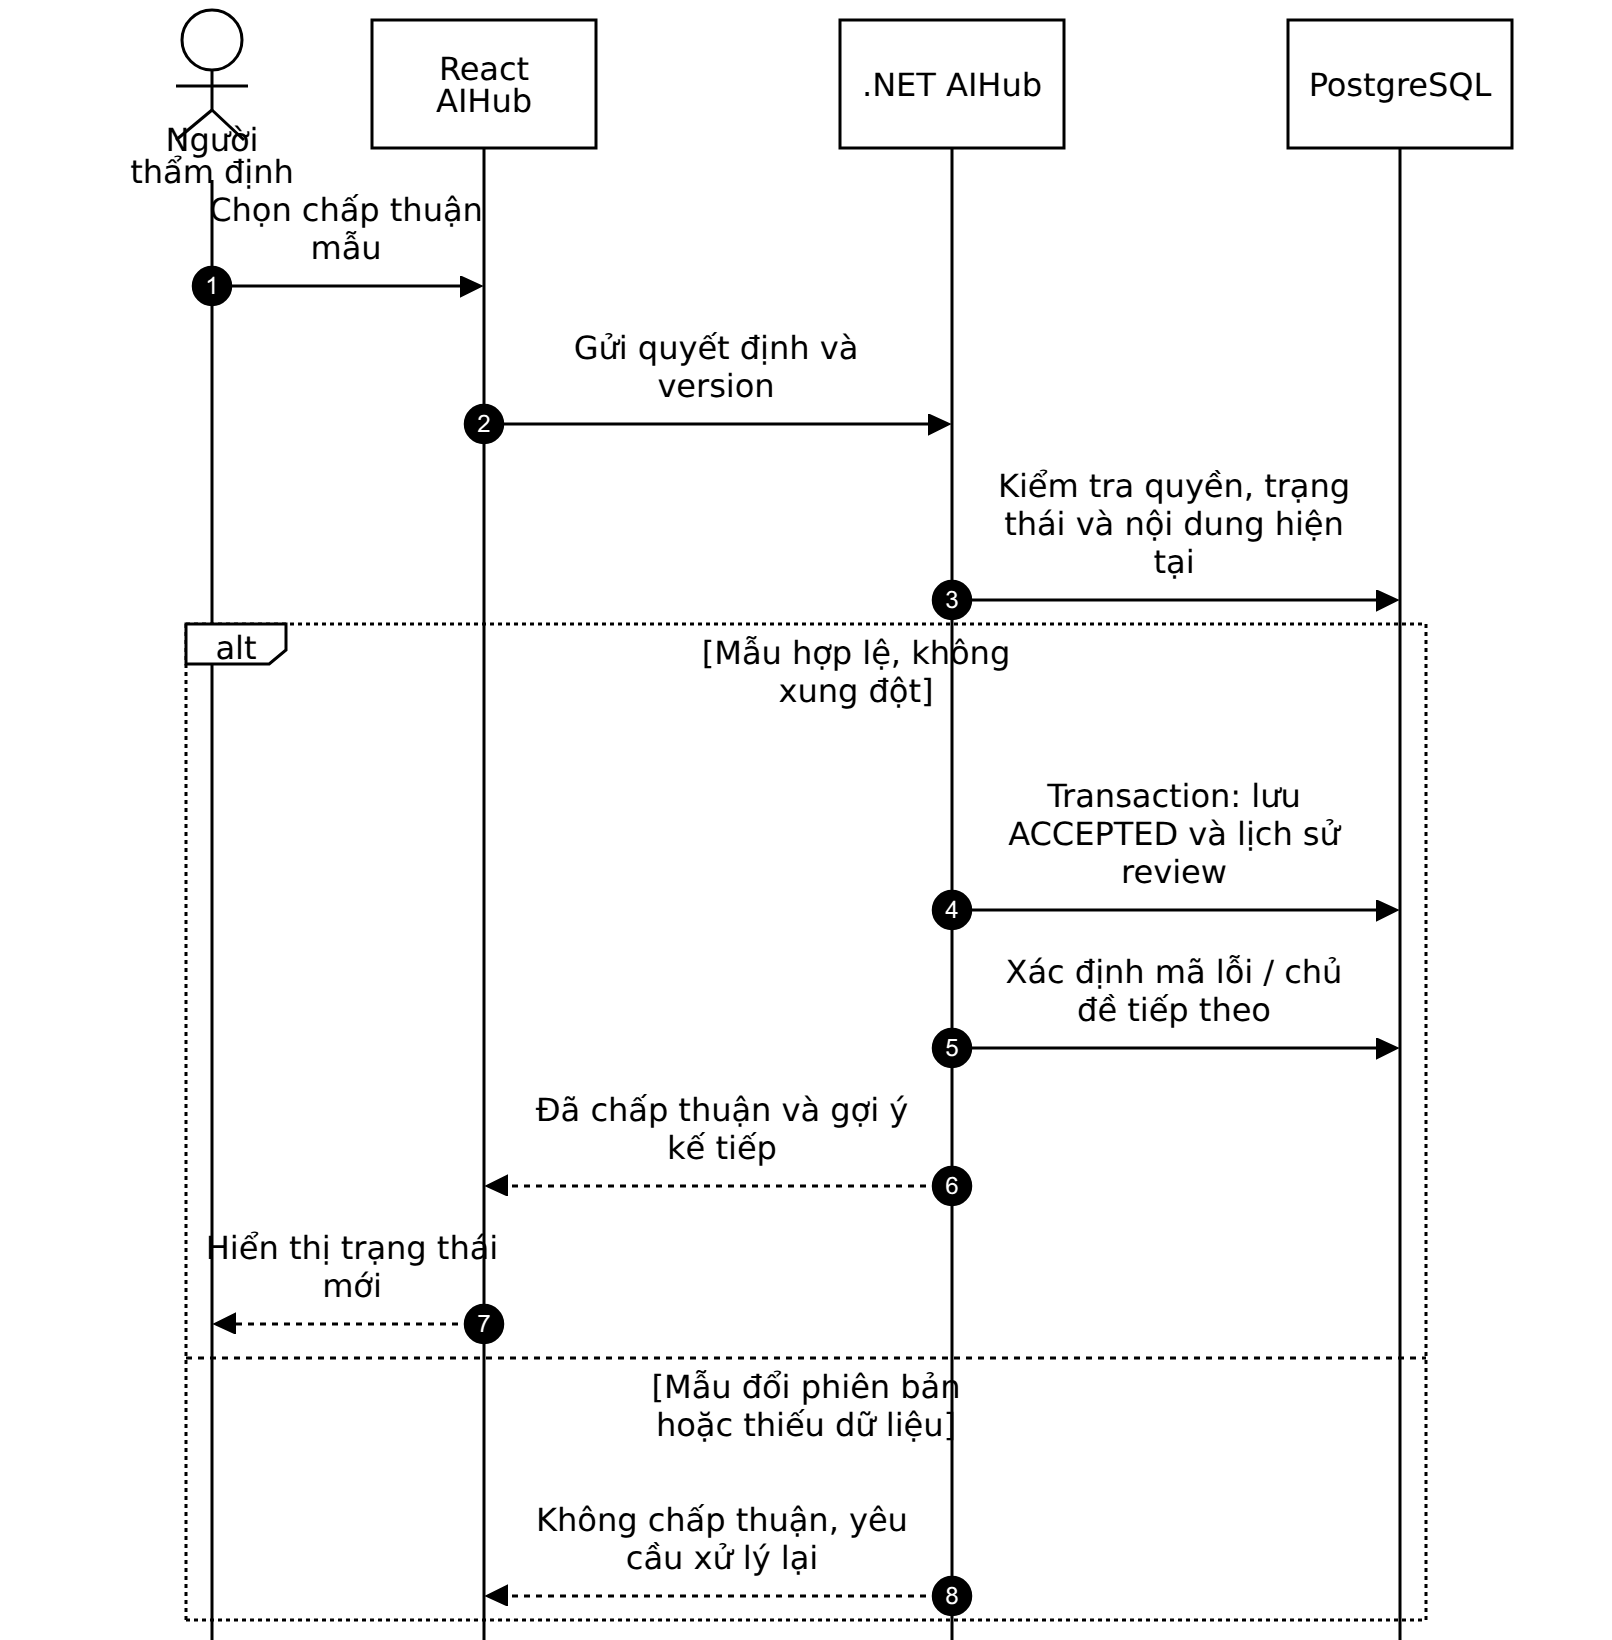
\includegraphics[width=\linewidth,height=.77\textheight,keepaspectratio]{Images/Sequence/AIHub/sequence_uc09_accept_sample.png}
\caption{Sequence diagram AIHub UC09 — Chấp thuận mẫu học thuật}
\label{sequence:aihub:sequence_uc09_accept_sample}
\end{figure}

Quyết định chấp thuận là giao dịch độc lập, có kiểm tra trạng thái và phiên bản trước khi xoay vòng lỗi.

\clearpage
\paragraph*{UC10. Từ chối mẫu học thuật}

\begin{figure}[H]
\centering
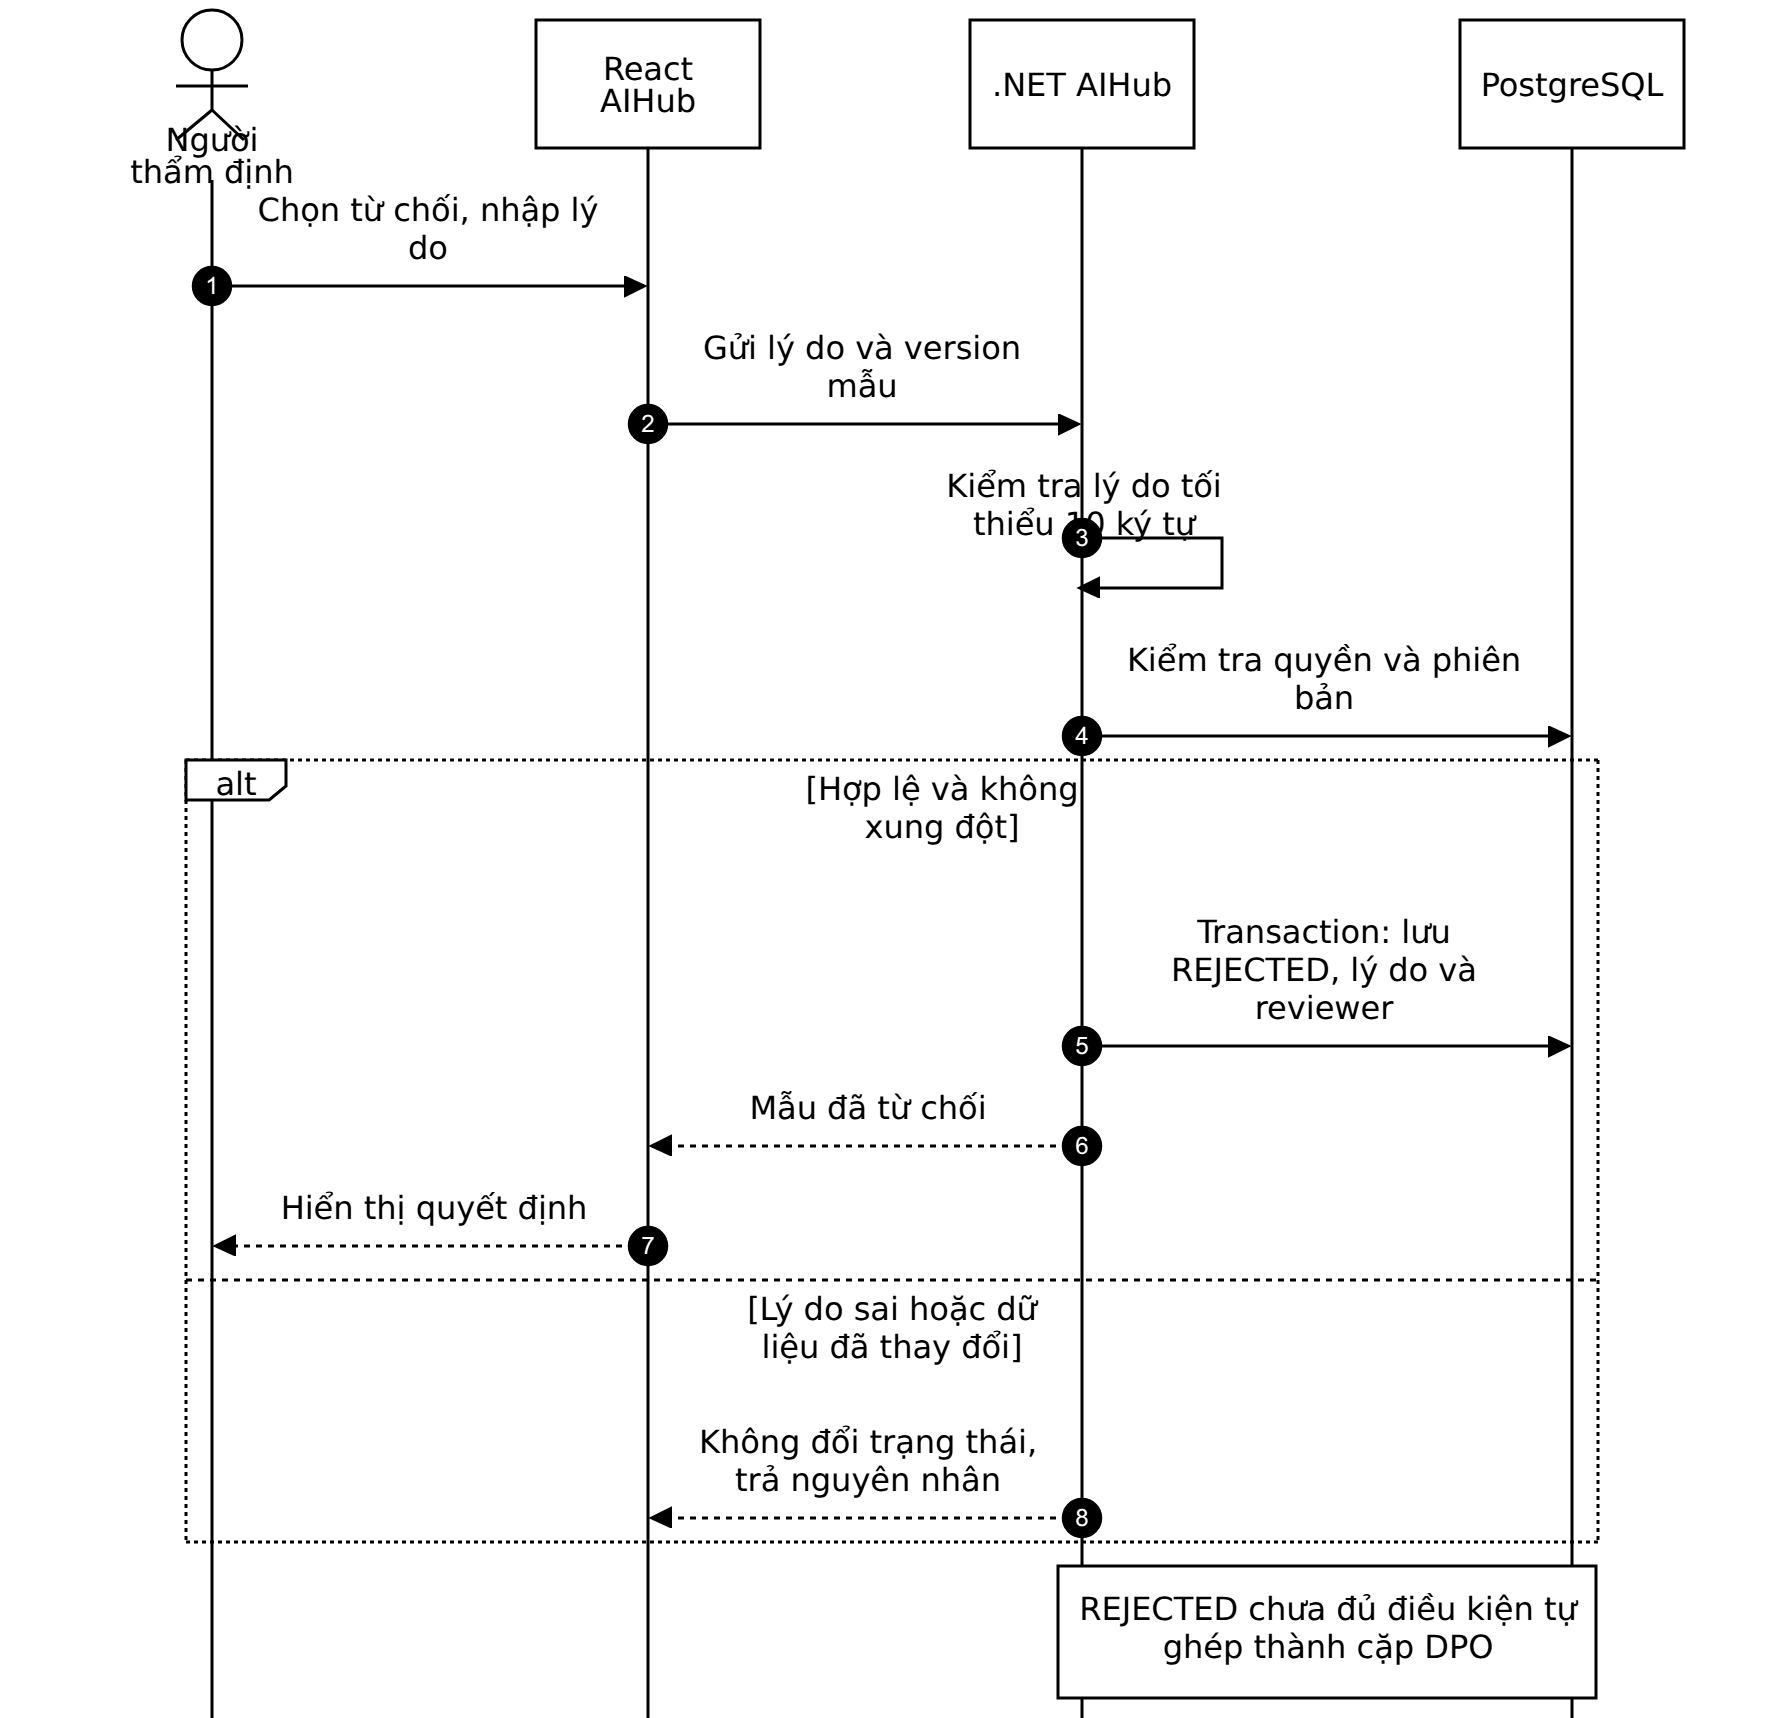
\includegraphics[width=\linewidth,height=.77\textheight,keepaspectratio]{Images/Sequence/AIHub/sequence_uc10_reject_sample.png}
\caption{Sequence diagram AIHub UC10 — Từ chối mẫu học thuật}
\label{sequence:aihub:sequence_uc10_reject_sample}
\end{figure}

Từ chối bảo toàn nội dung gốc và lý do; trạng thái REJECTED không tự biến mẫu thành dữ liệu DPO hợp lệ.

\clearpage
\paragraph*{UC11. Quản lý kho mẫu học thuật}

\begin{figure}[H]
\centering
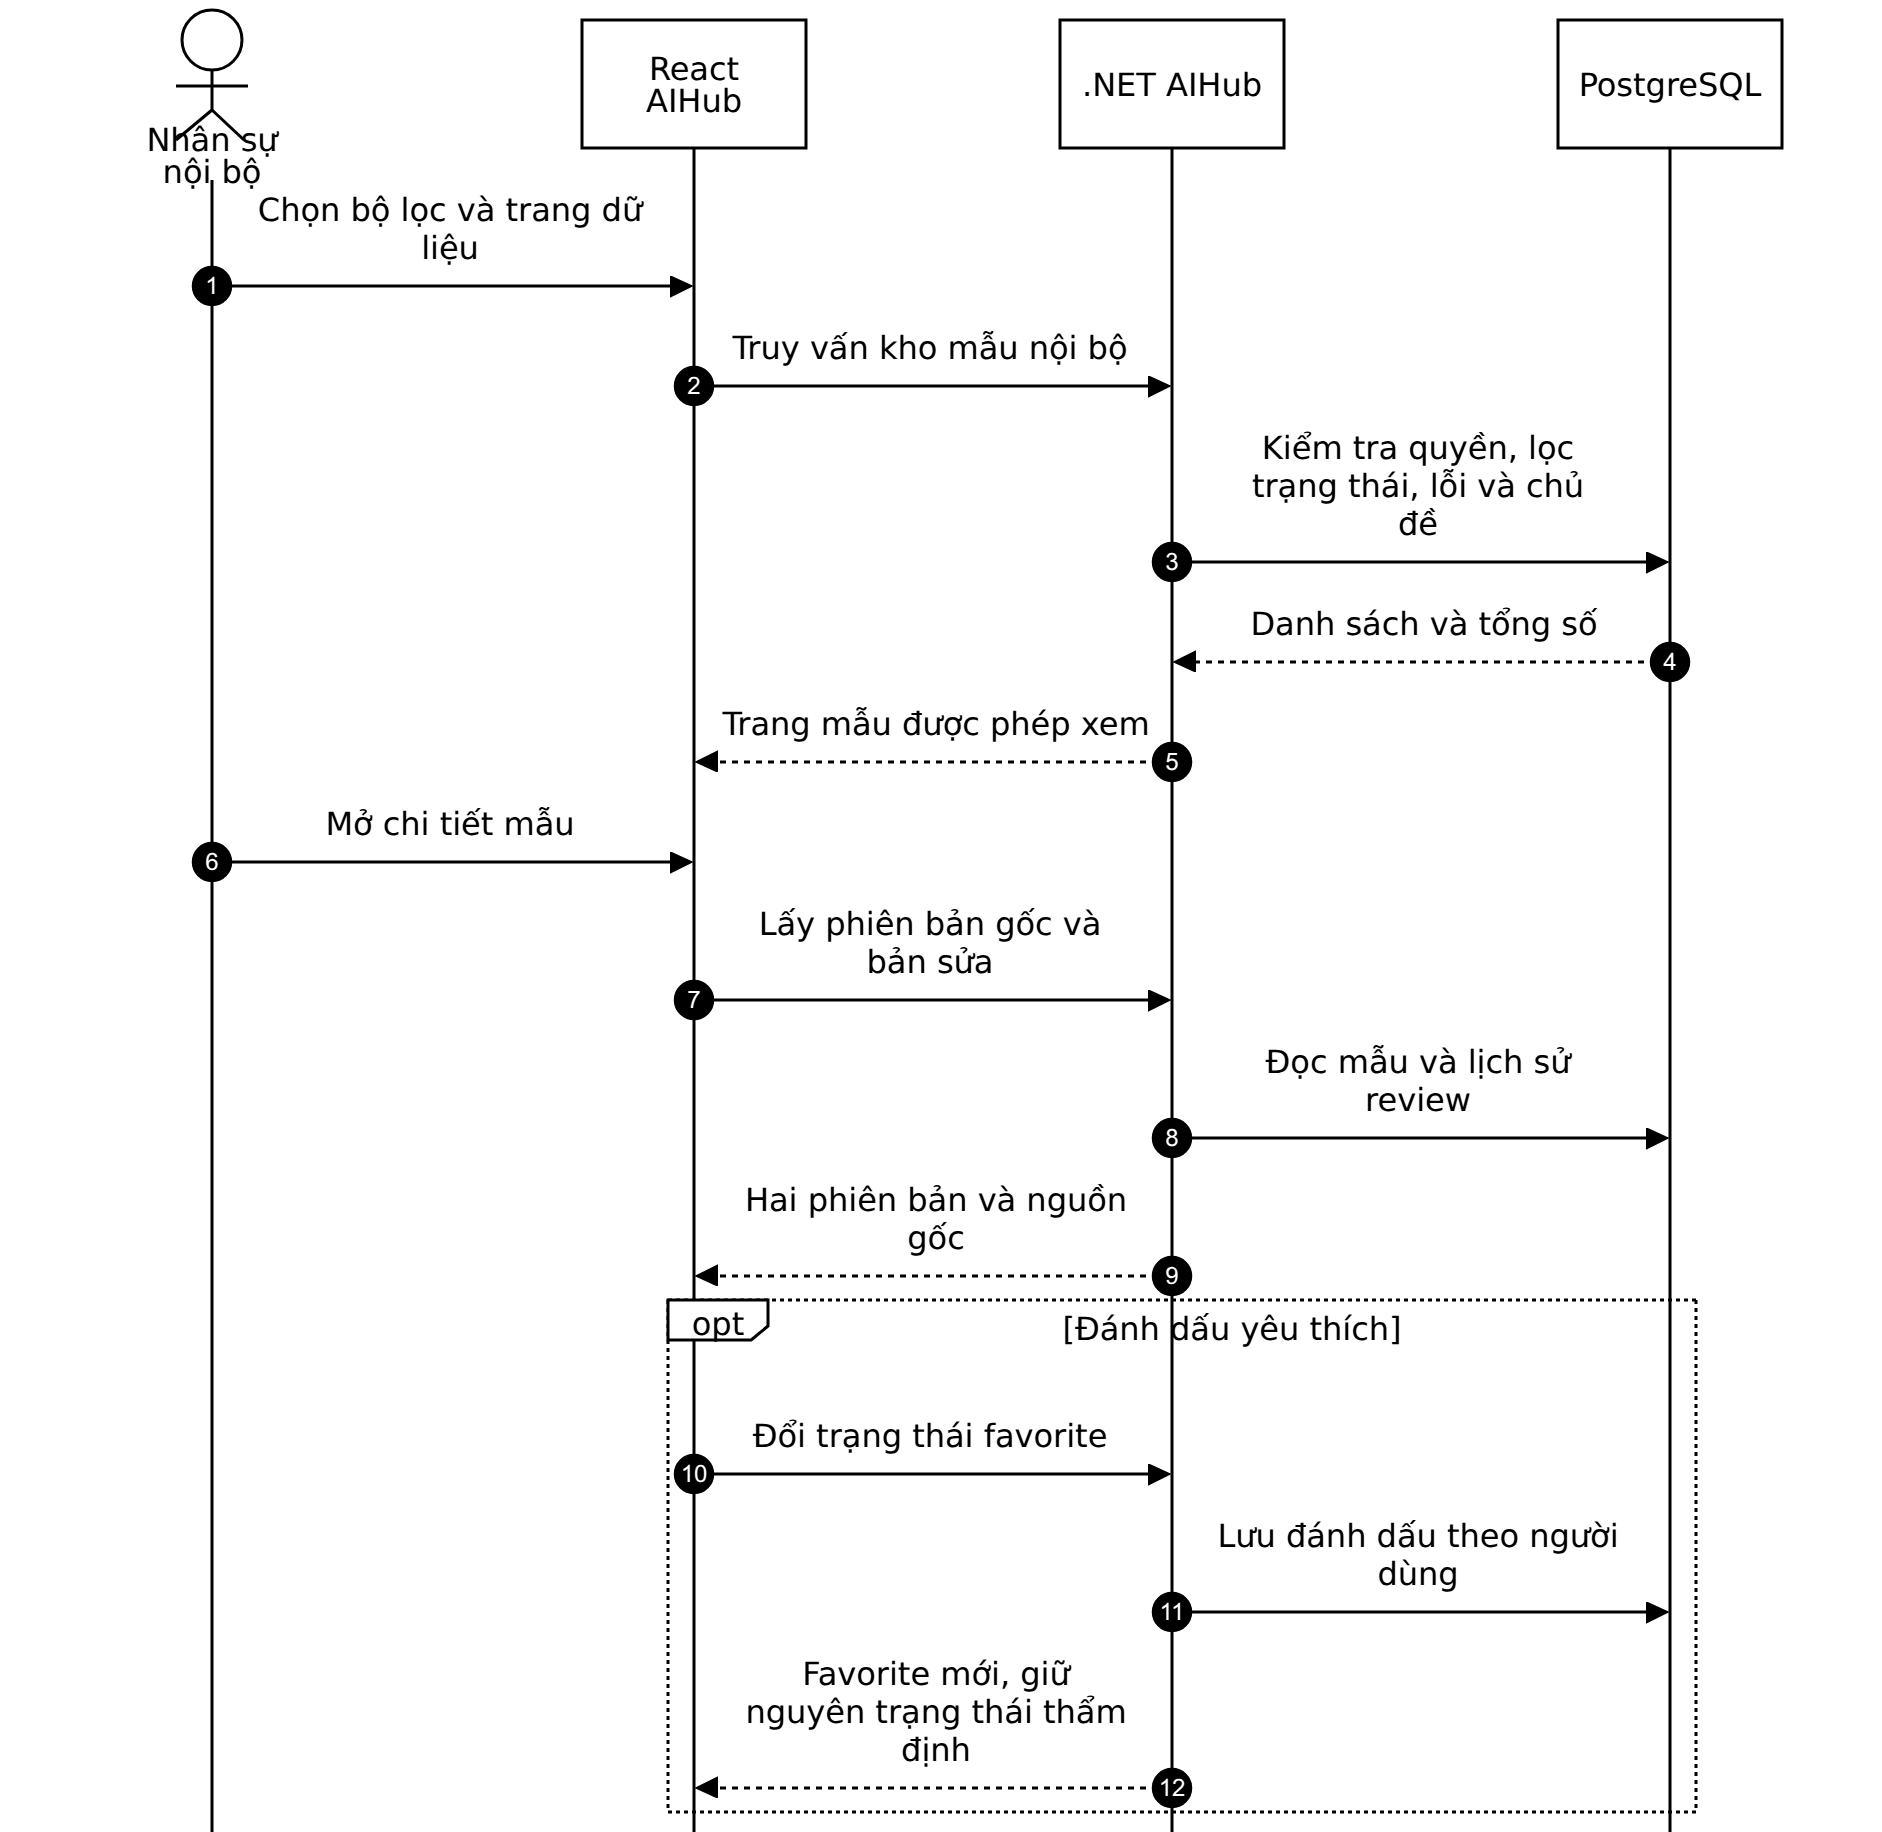
\includegraphics[width=\linewidth,height=.77\textheight,keepaspectratio]{Images/Sequence/AIHub/sequence_uc11_academic_inventory.png}
\caption{Sequence diagram AIHub UC11 — Quản lý kho mẫu học thuật}
\label{sequence:aihub:sequence_uc11_academic_inventory}
\end{figure}

Kho mẫu tách nội dung gốc, bản sửa và lịch sử; đánh dấu yêu thích không thay đổi quyết định thẩm định.

\clearpage
\paragraph*{UC12. Cấu hình mẫu Prompt}

\begin{figure}[H]
\centering
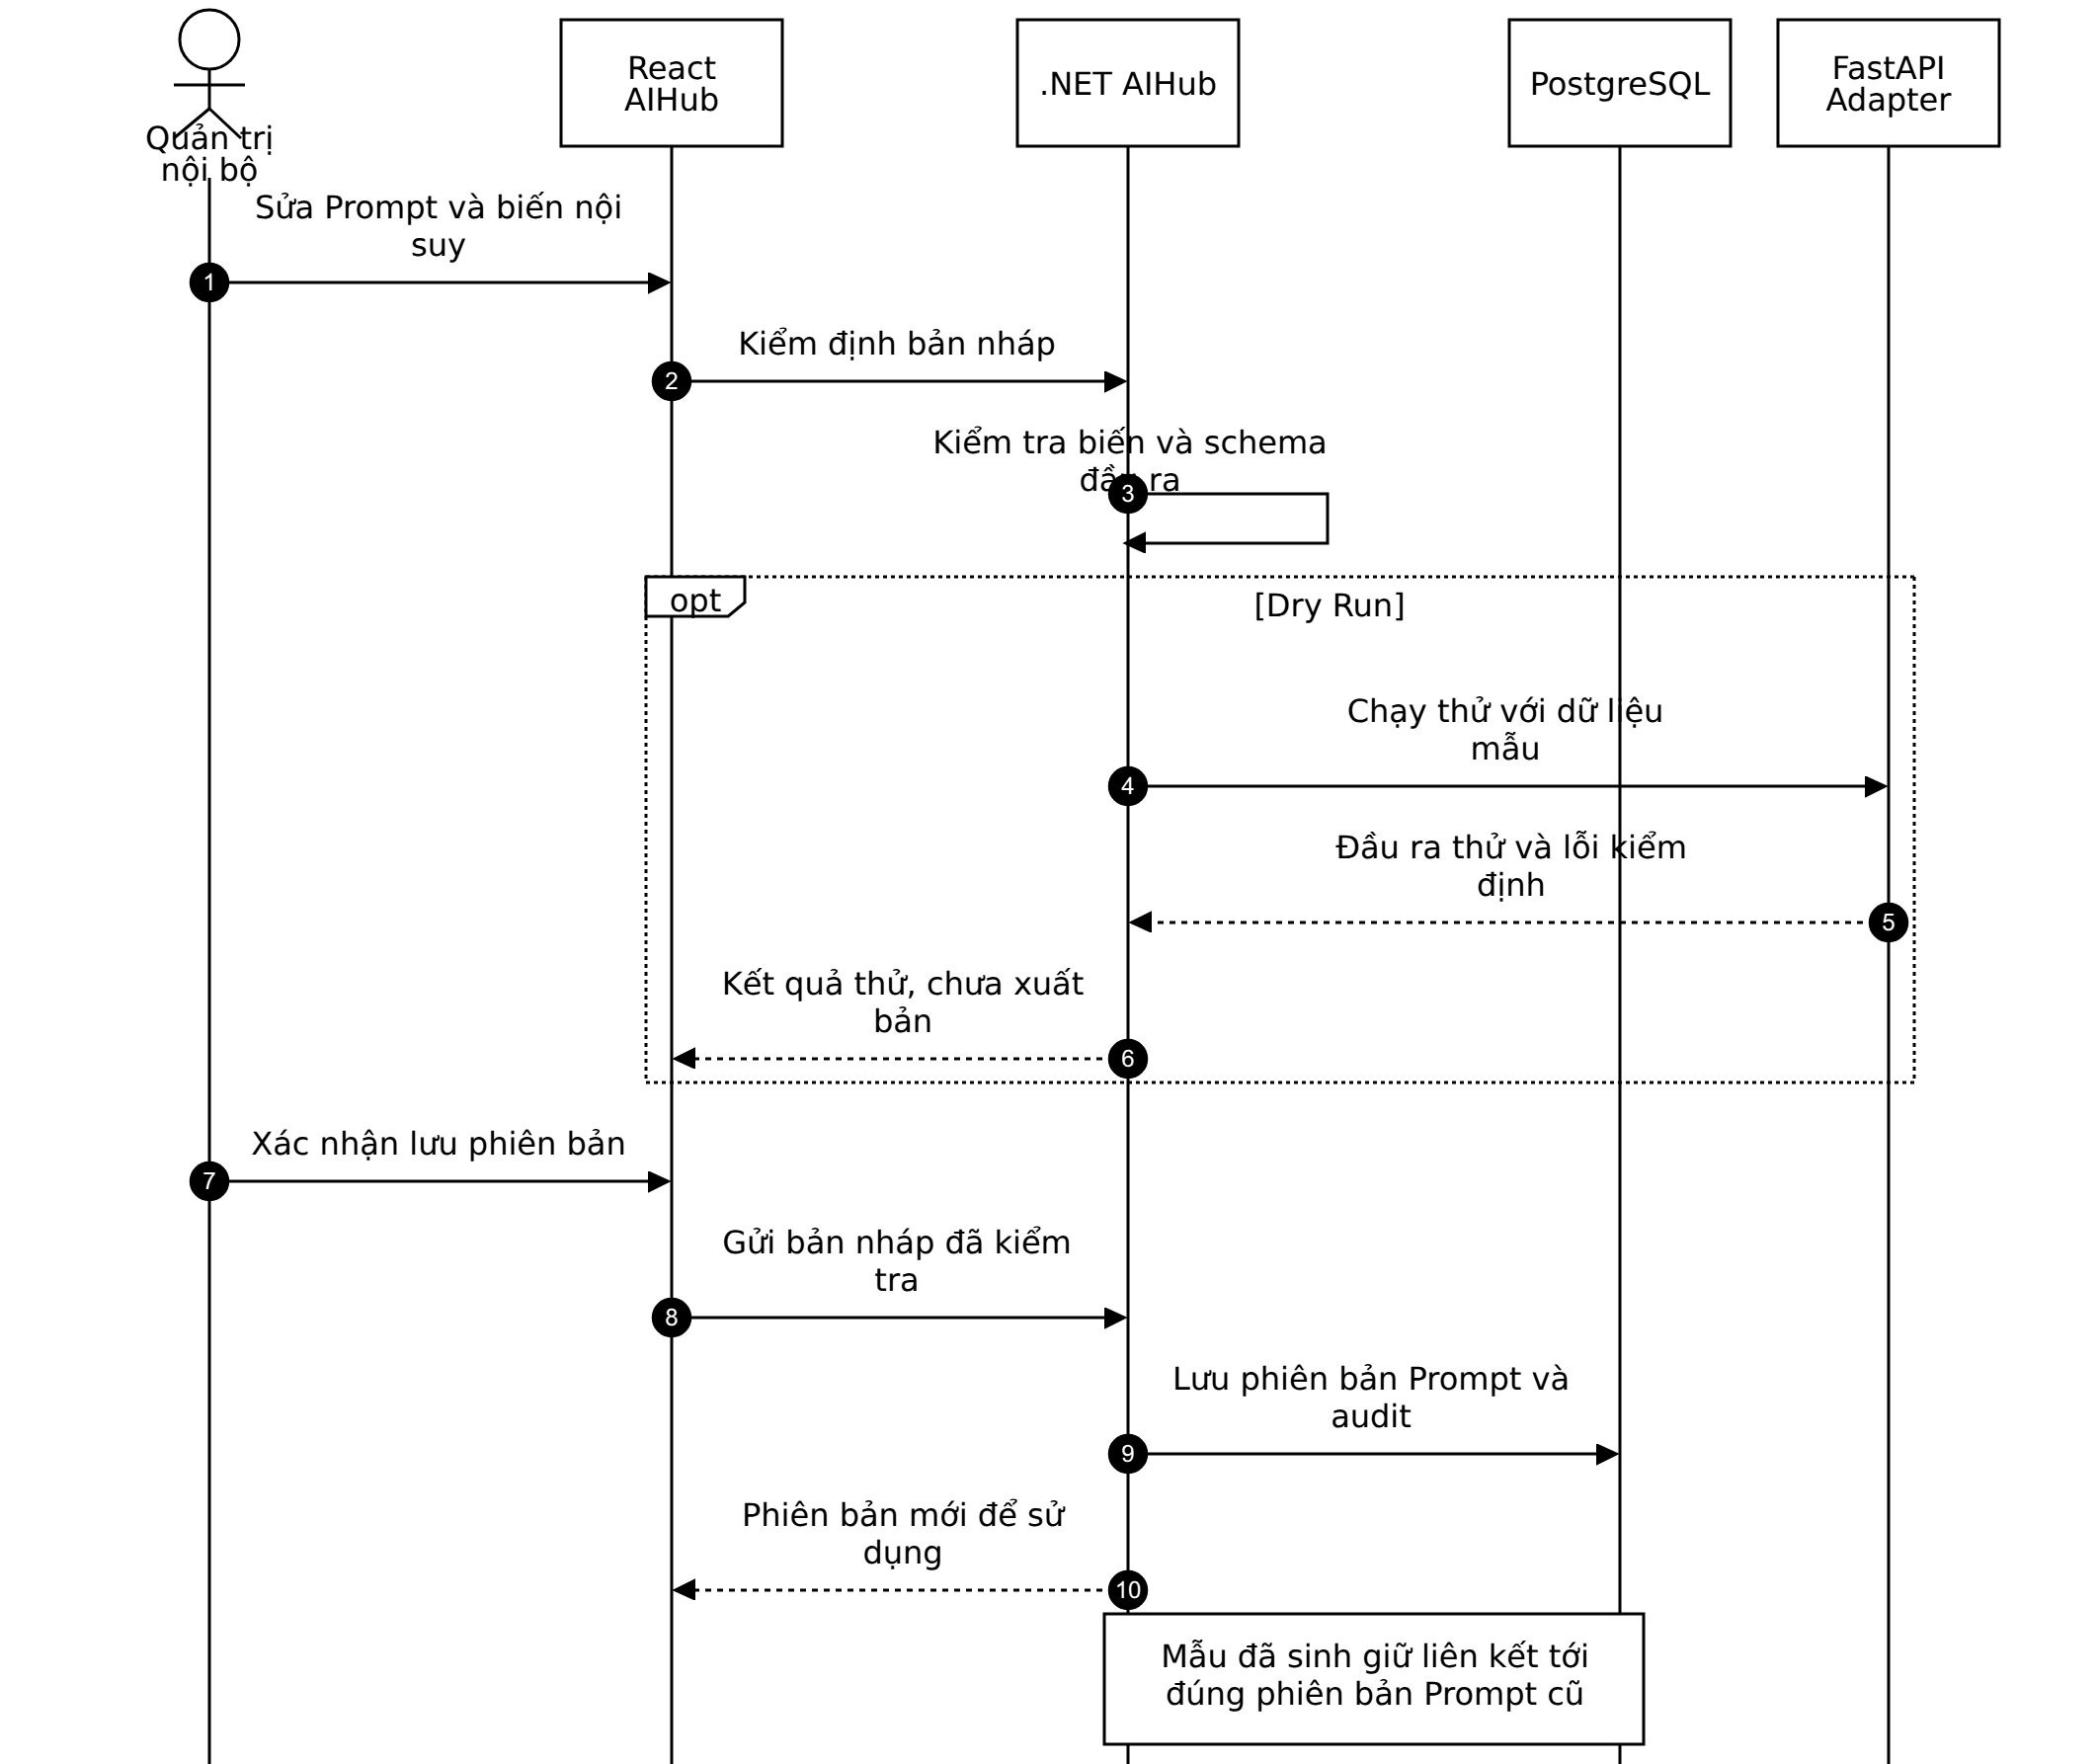
\includegraphics[width=\linewidth,height=.77\textheight,keepaspectratio]{Images/Sequence/AIHub/sequence_uc12_prompt_templates.png}
\caption{Sequence diagram AIHub UC12 — Cấu hình mẫu Prompt}
\label{sequence:aihub:sequence_uc12_prompt_templates}
\end{figure}

Dry Run không xuất bản cấu hình; Prompt được lưu phiên bản để bảo toàn khả năng truy vết mẫu.

\clearpage
\paragraph*{UC13. Cấu hình chuỗi mô hình dự phòng}

\begin{figure}[H]
\centering
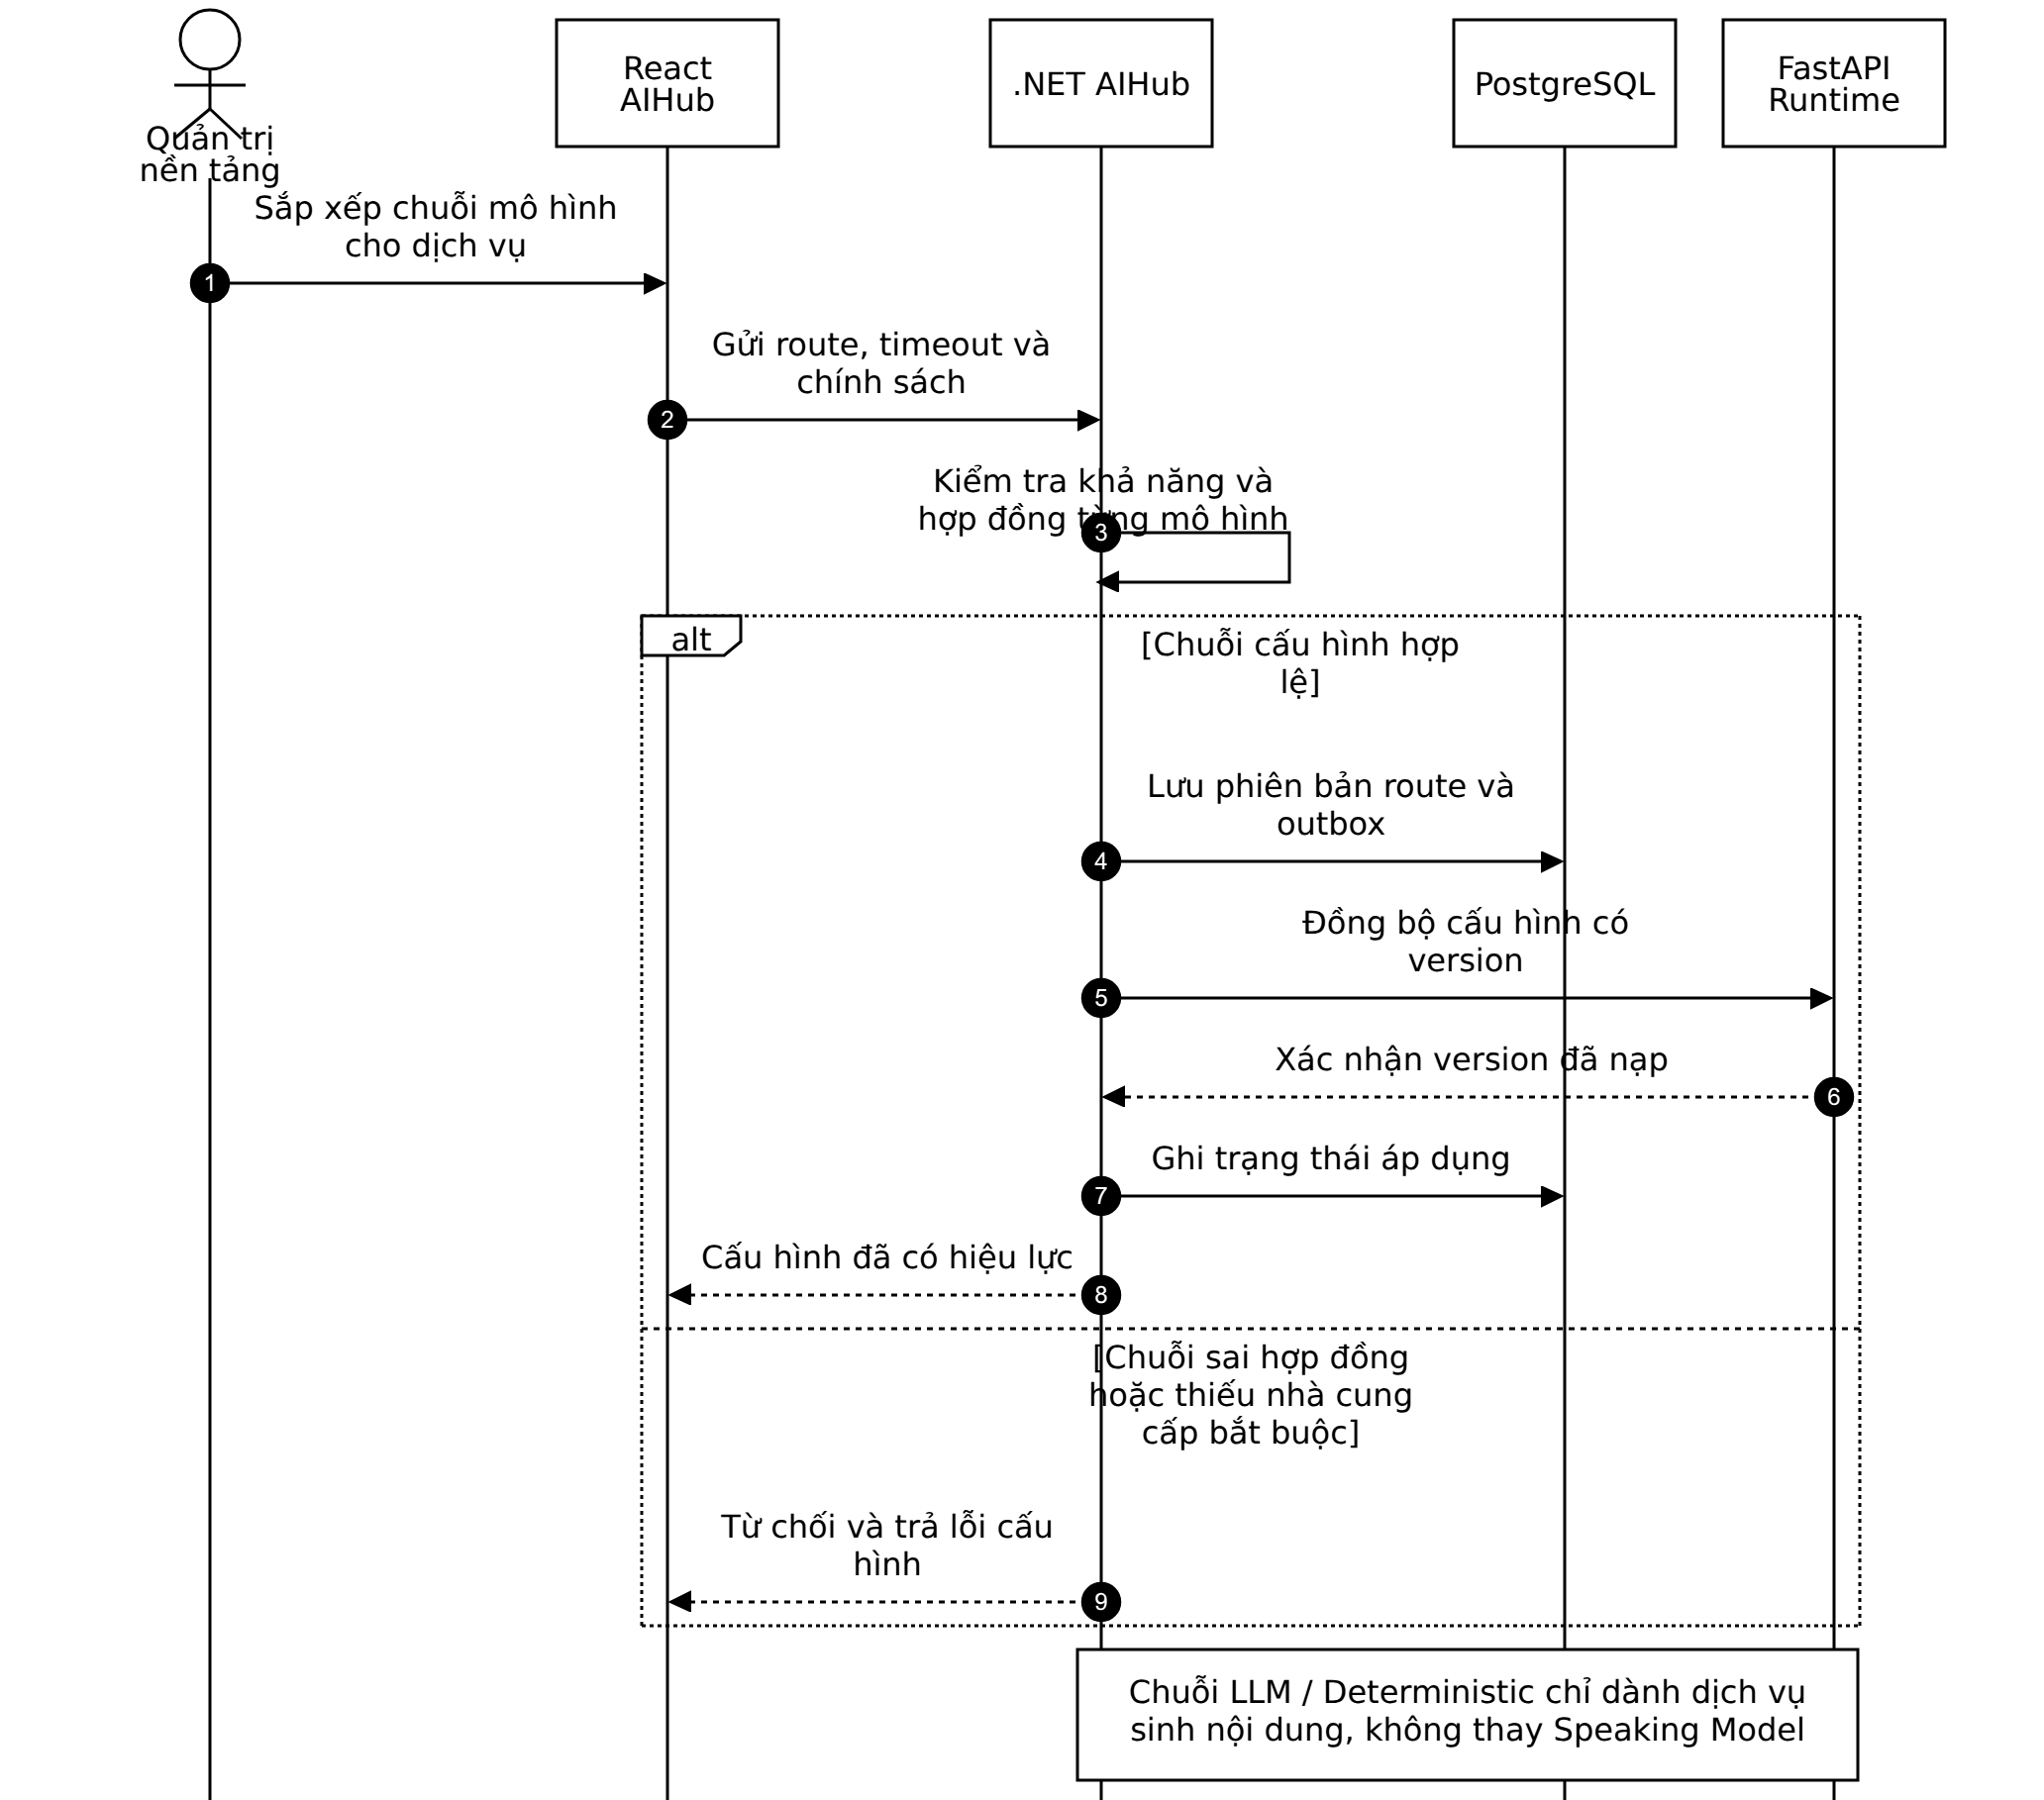
\includegraphics[width=\linewidth,height=.77\textheight,keepaspectratio]{Images/Sequence/AIHub/sequence_uc13_model_fallback.png}
\caption{Sequence diagram AIHub UC13 — Cấu hình chuỗi mô hình dự phòng}
\label{sequence:aihub:sequence_uc13_model_fallback}
\end{figure}

Chỉ công bố route đã kiểm định; dự phòng cho sinh nội dung không mặc nhiên thay thế mô hình chấm Speaking.

\clearpage
\paragraph*{UC14. Xuất dữ liệu SFT và DPO}

\begin{figure}[H]
\centering
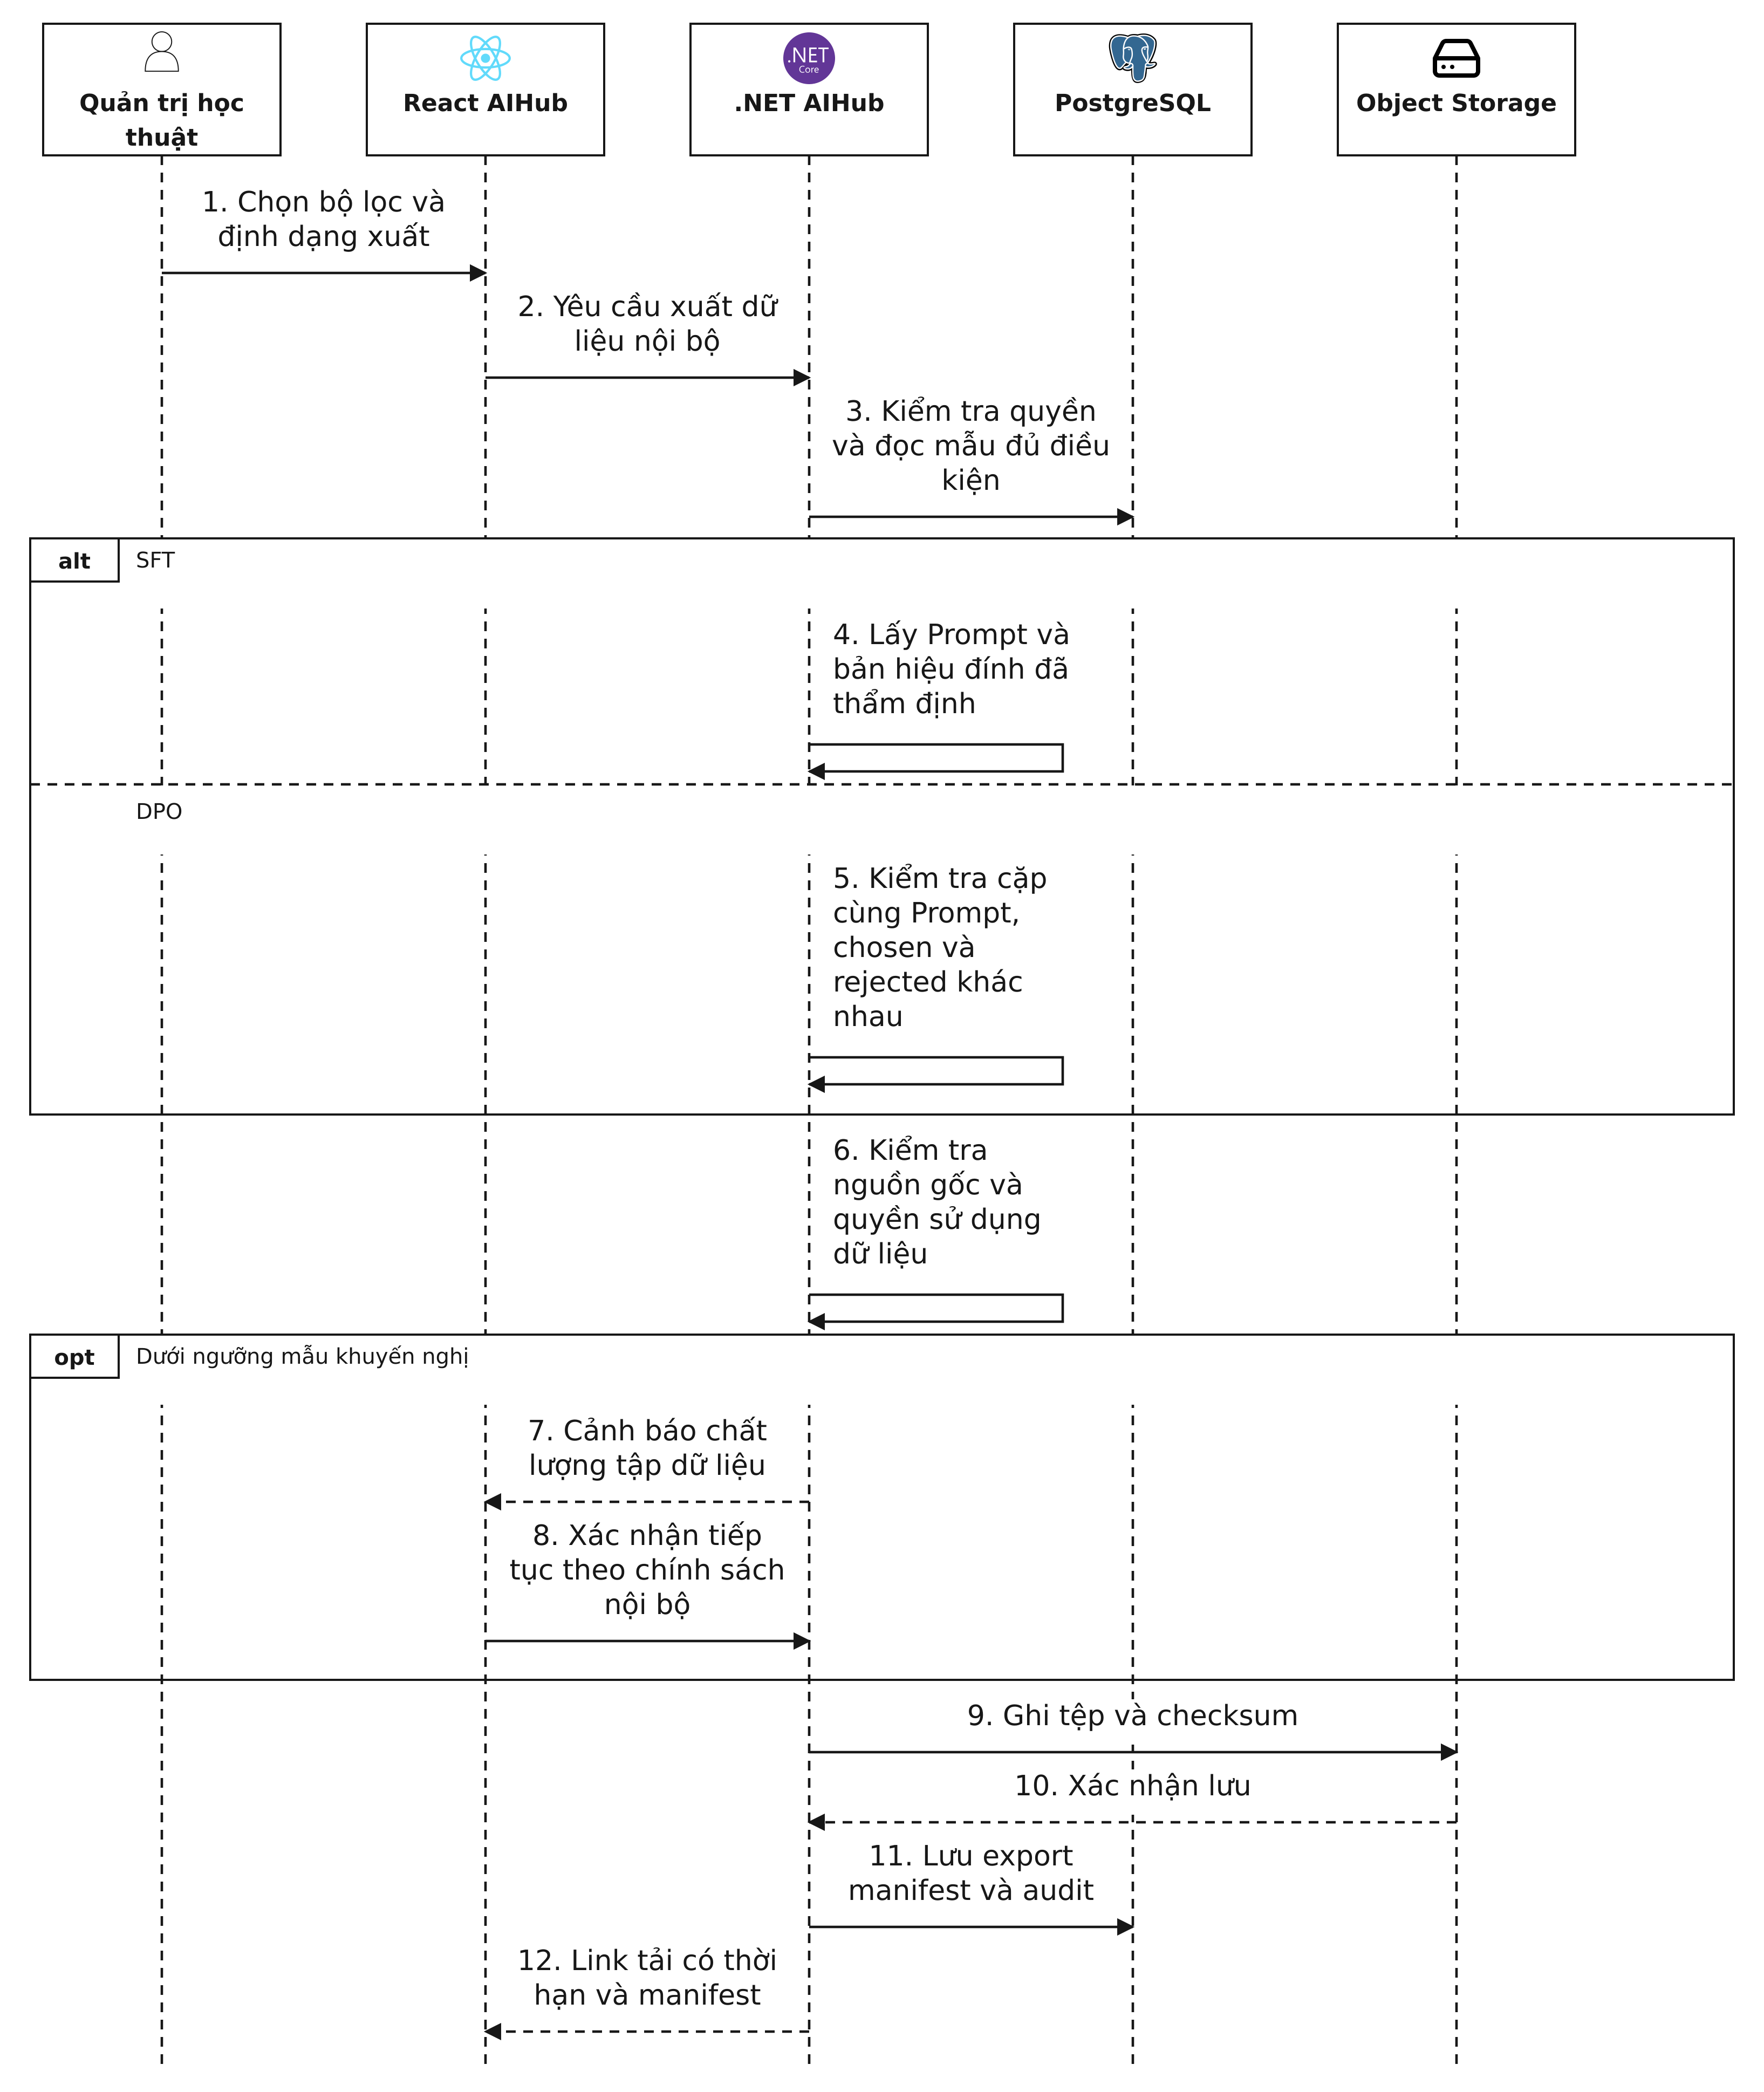
\includegraphics[width=\linewidth,height=.77\textheight,keepaspectratio]{Images/Sequence/AIHub/sequence_uc14_export_datasets.png}
\caption{Sequence diagram AIHub UC14 — Xuất dữ liệu SFT và DPO}
\label{sequence:aihub:sequence_uc14_export_datasets}
\end{figure}

Xuất dữ liệu kiểm tra nguồn gốc và cấu trúc cặp; manifest lưu đầy đủ mẫu và phiên bản được chọn.

\clearpage
\paragraph*{UC15. Phân tích lỗi mô hình}

\begin{figure}[H]
\centering
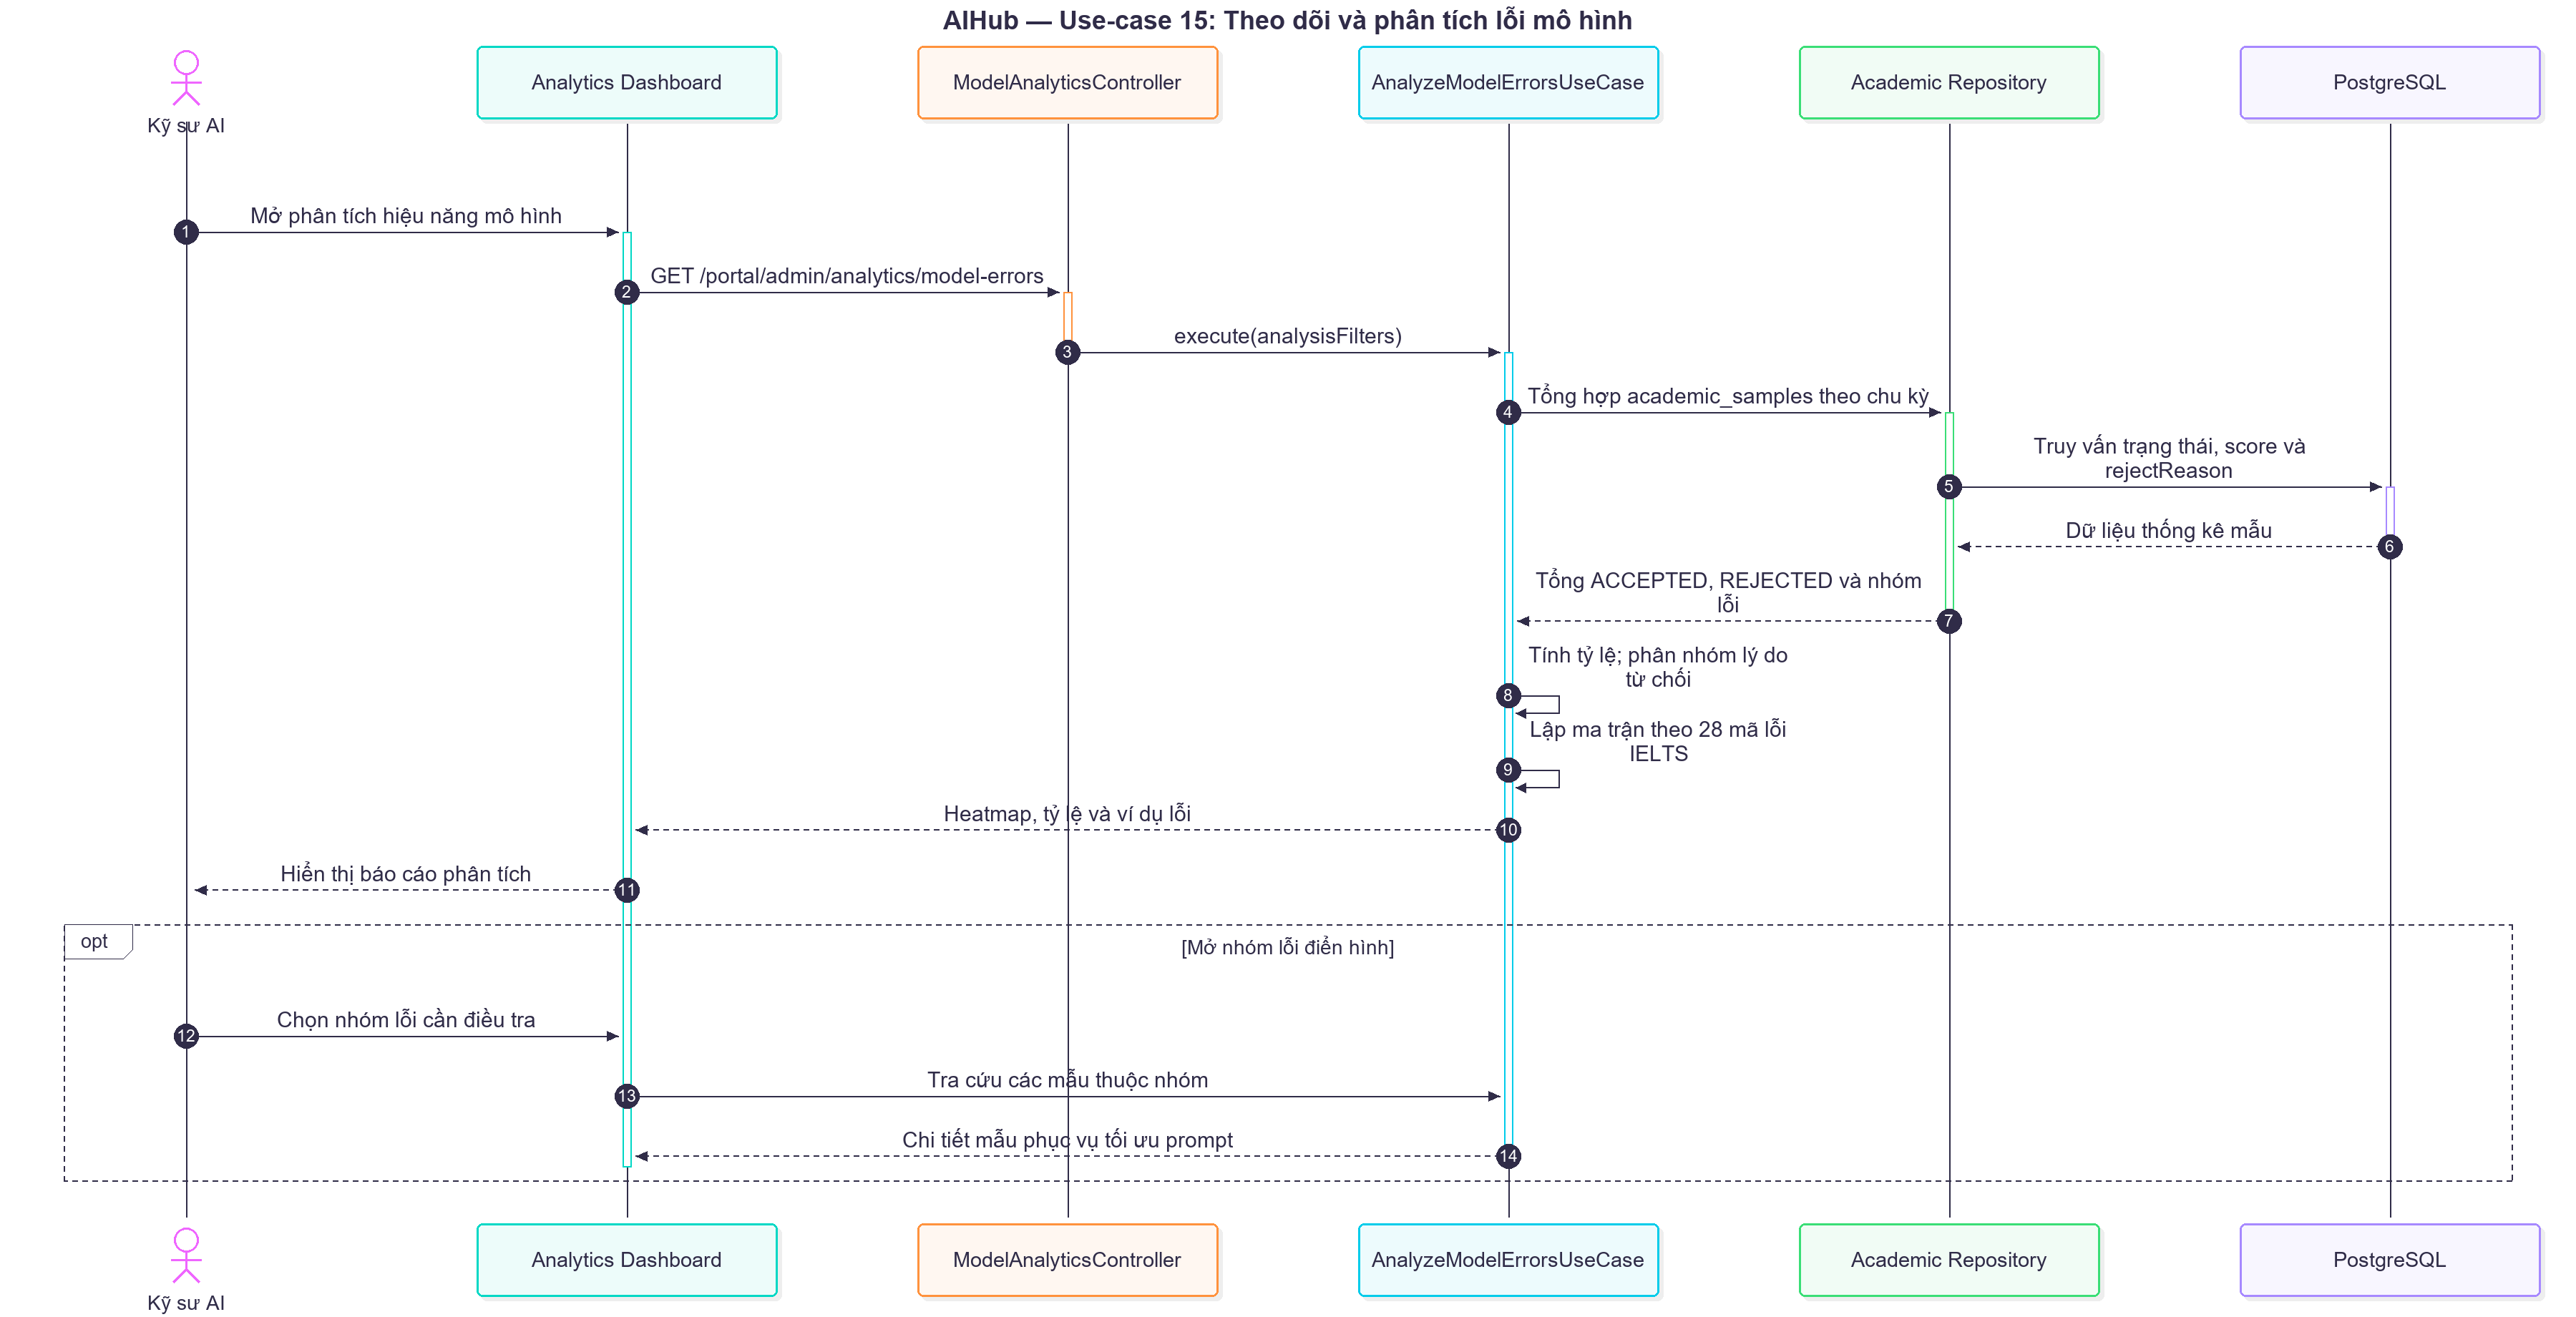
\includegraphics[width=\linewidth,height=.77\textheight,keepaspectratio]{Images/Sequence/AIHub/sequence_uc15_model_error_analysis.png}
\caption{Sequence diagram AIHub UC15 — Phân tích lỗi mô hình}
\label{sequence:aihub:sequence_uc15_model_error_analysis}
\end{figure}

Thống kê thể hiện số mẫu và phiên bản; mẫu nháp không làm sai mẫu số của tỷ lệ thẩm định.

\clearpage
\paragraph*{UC16. Quản lý thành viên tổ chức}

\begin{figure}[H]
\centering
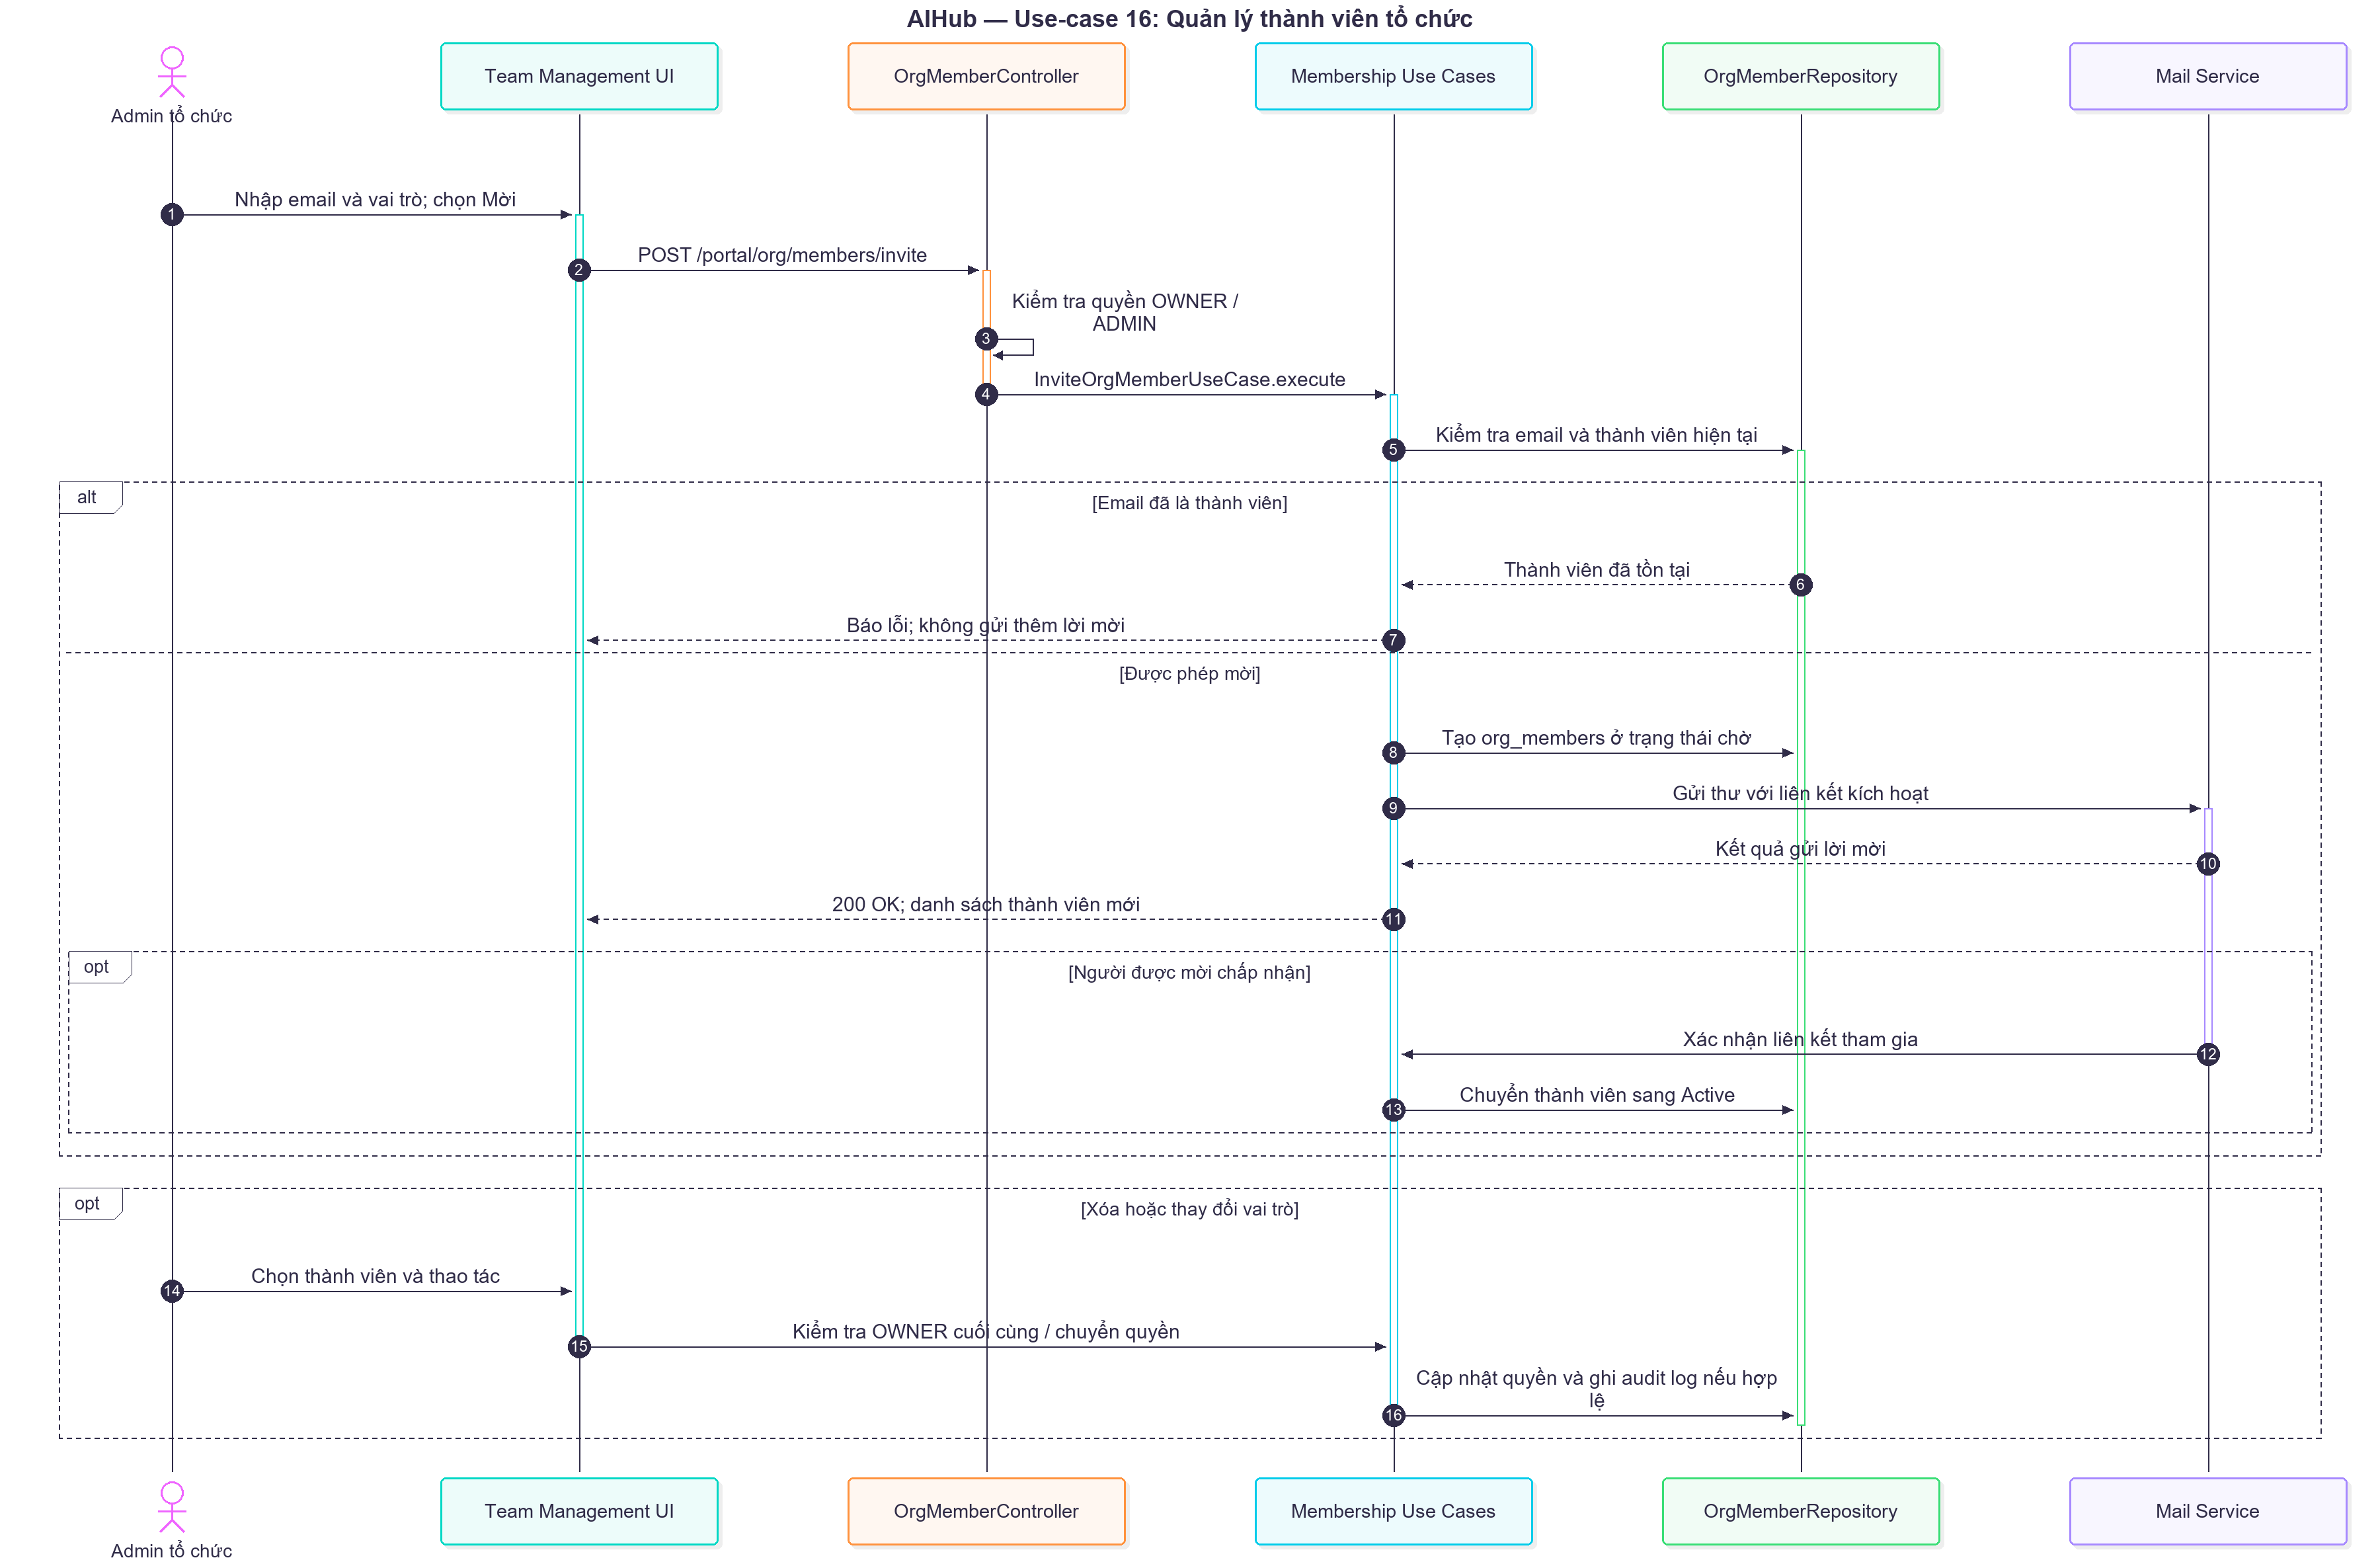
\includegraphics[width=\linewidth,height=.77\textheight,keepaspectratio]{Images/Sequence/AIHub/sequence_uc16_organization_members.png}
\caption{Sequence diagram AIHub UC16 — Quản lý thành viên tổ chức}
\label{sequence:aihub:sequence_uc16_organization_members}
\end{figure}

Mọi thay đổi giới hạn theo tổ chức; chuyển Owner là giao dịch có xác thực bổ sung và không để mất Owner.

\clearpage
\paragraph*{UC17. Quản trị gói và hạn mức}

\begin{figure}[H]
\centering
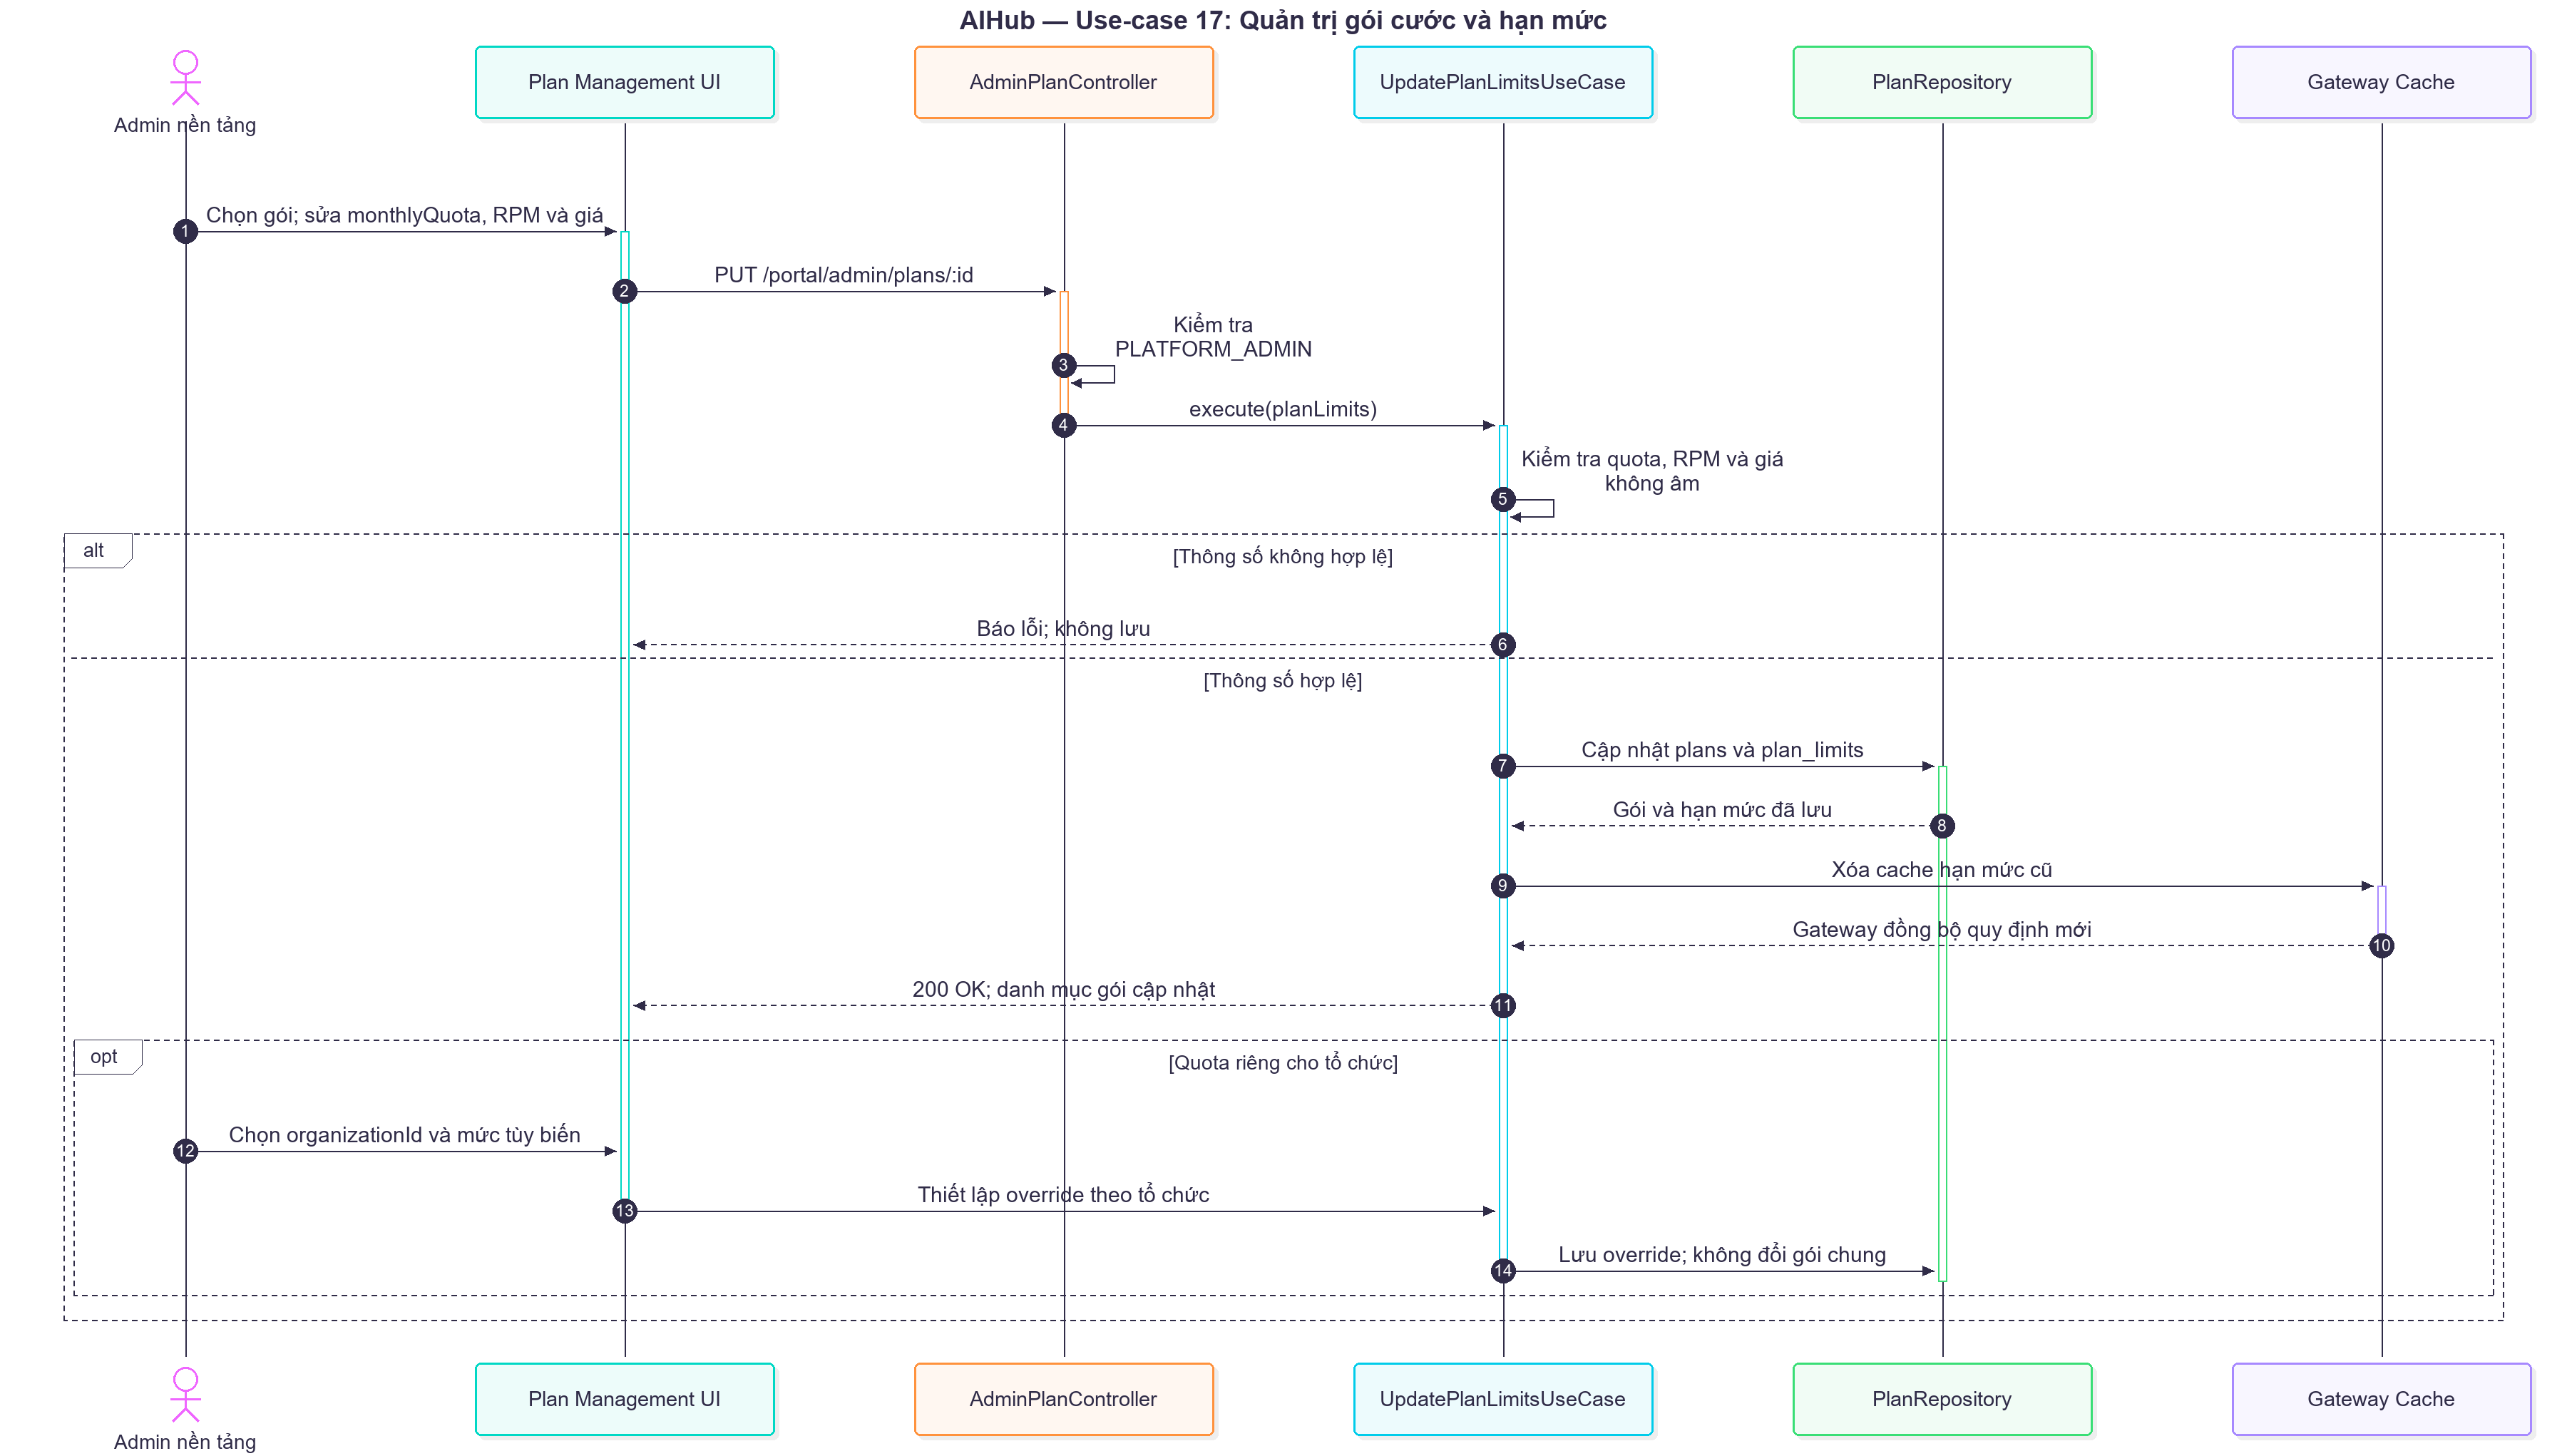
\includegraphics[width=\linewidth,height=.77\textheight,keepaspectratio]{Images/Sequence/AIHub/sequence_uc17_plans_quota.png}
\caption{Sequence diagram AIHub UC17 — Quản trị gói và hạn mức}
\label{sequence:aihub:sequence_uc17_plans_quota}
\end{figure}

Cập nhật gói và override là hai nghiệp vụ khác nhau; override không tác động số dư của tổ chức khác.

\clearpage
\paragraph*{UC18. Giám sát trạng thái hệ thống}

\begin{figure}[H]
\centering
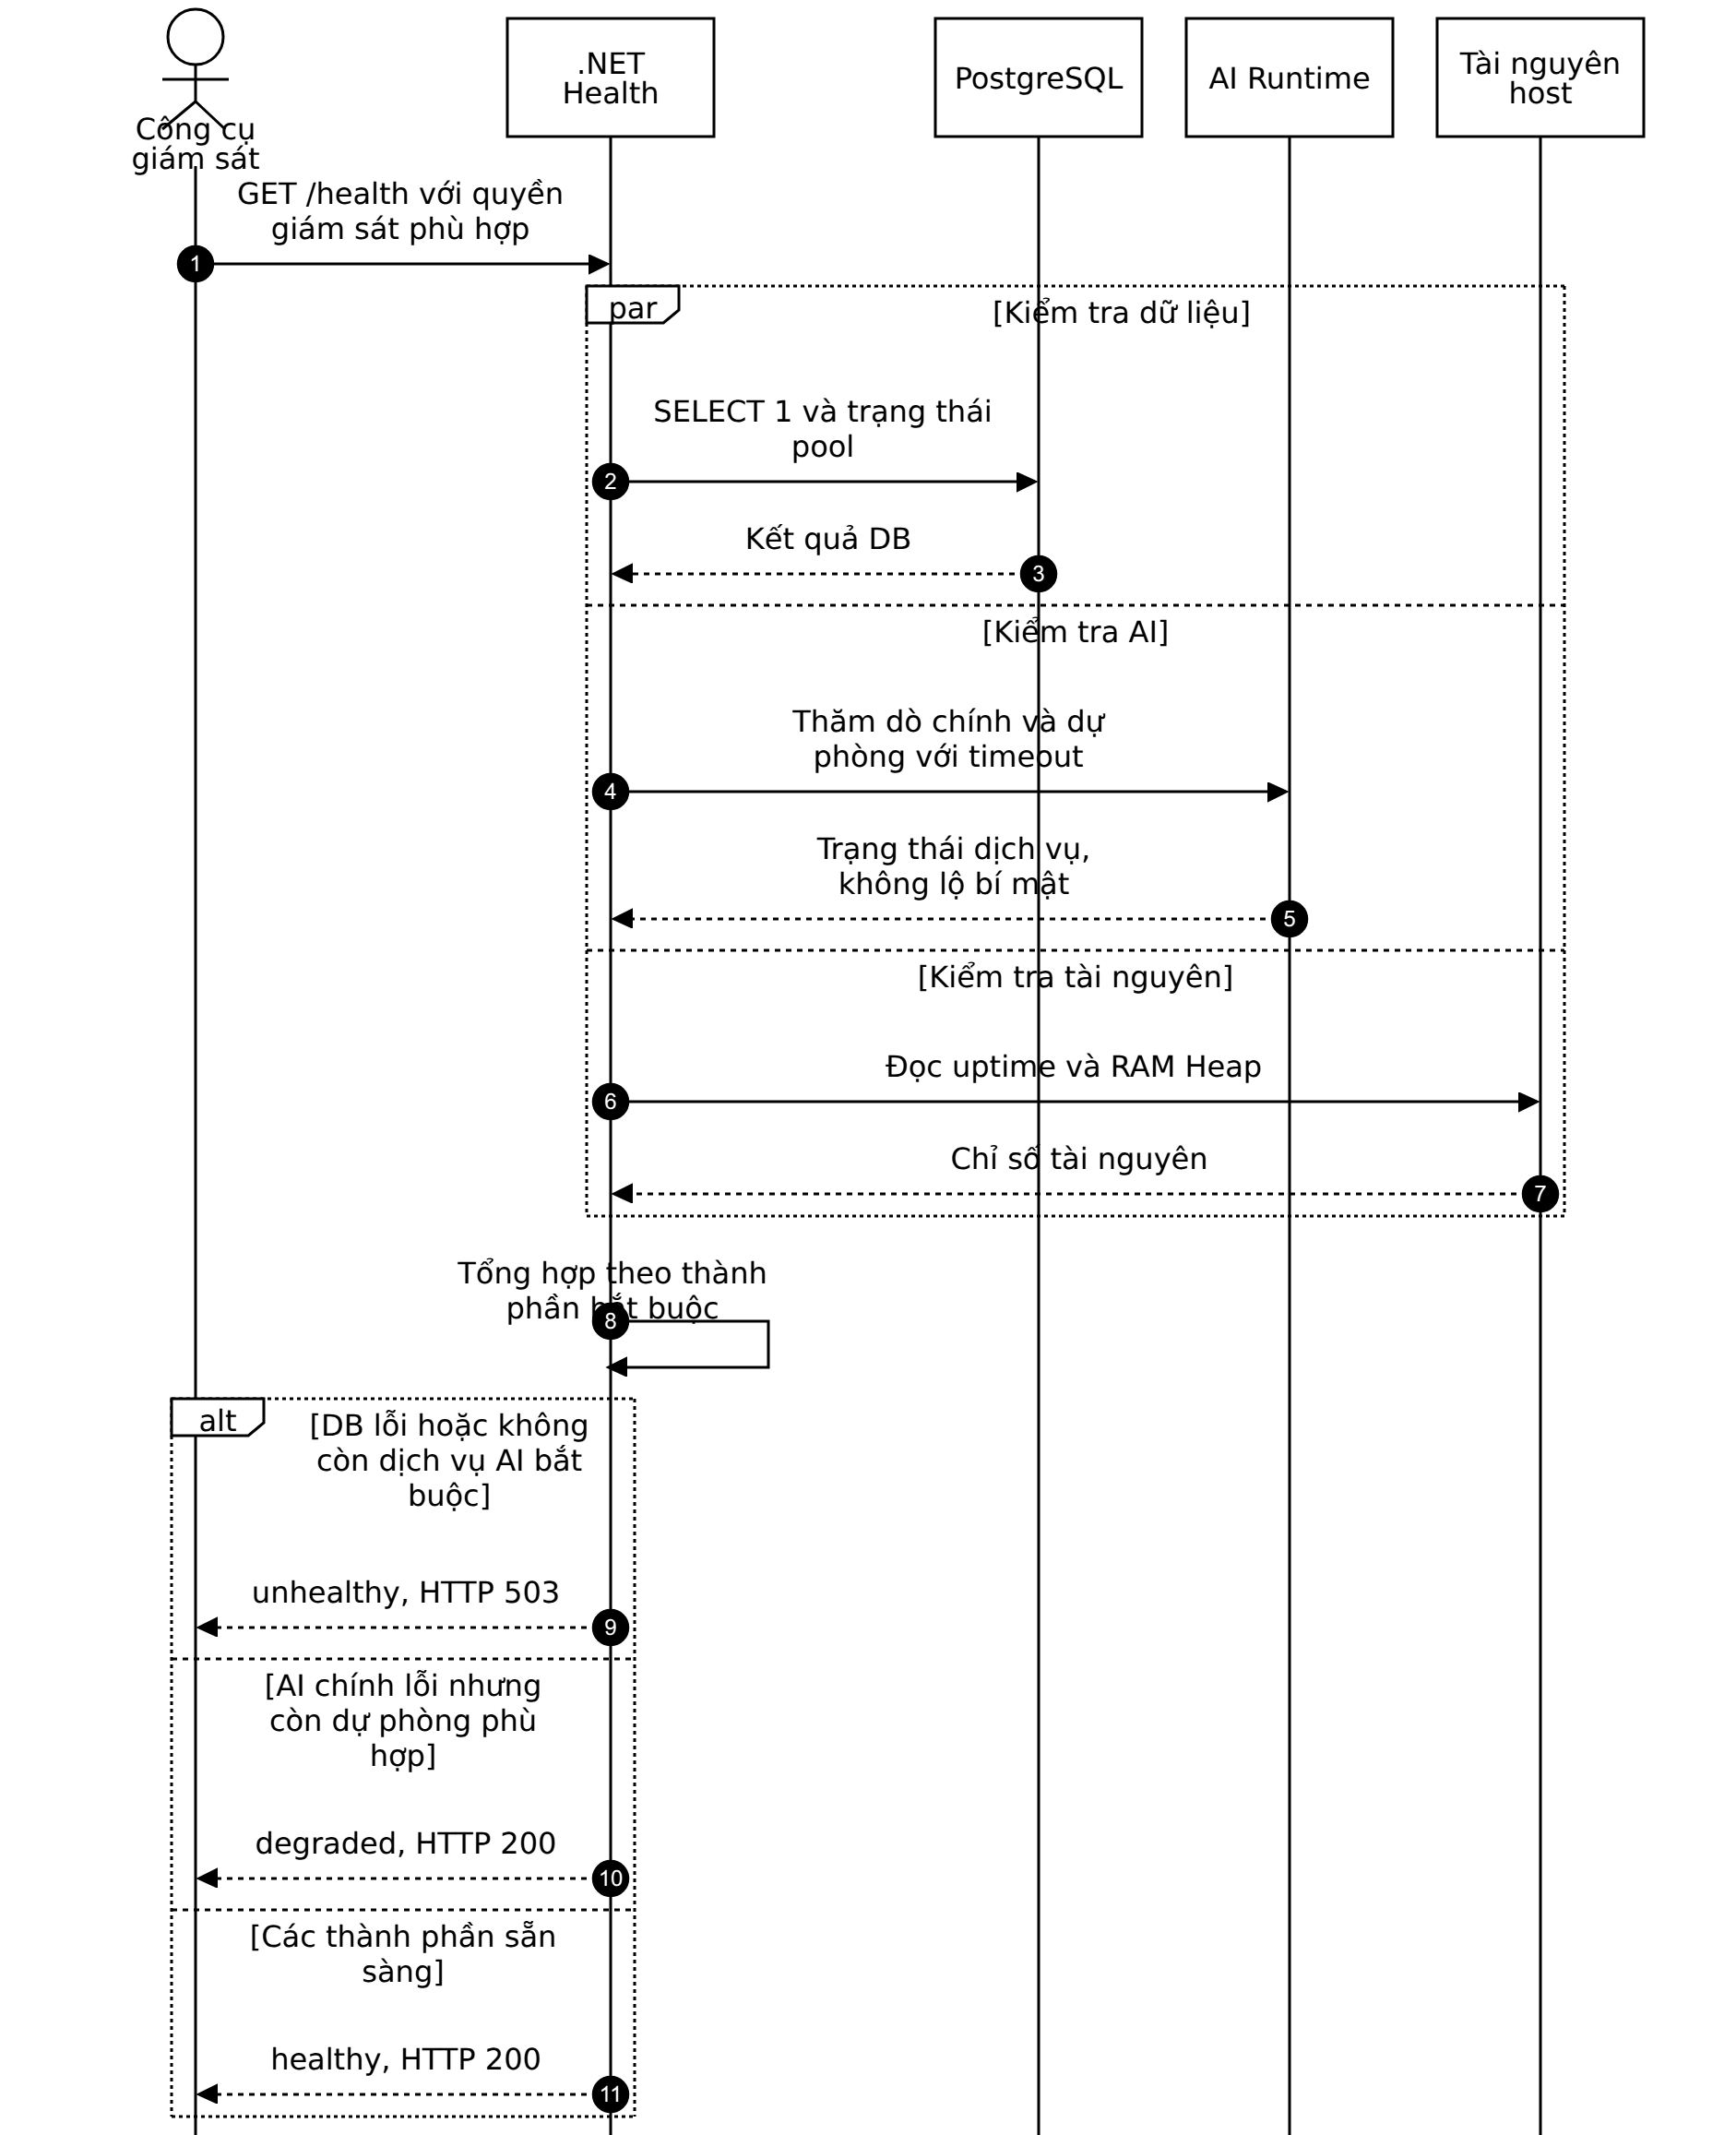
\includegraphics[width=\linewidth,height=.77\textheight,keepaspectratio]{Images/Sequence/AIHub/sequence_uc18_system_health.png}
\caption{Sequence diagram AIHub UC18 — Giám sát trạng thái hệ thống}
\label{sequence:aihub:sequence_uc18_system_health}
\end{figure}

Health tổng hợp kiểm tra có timeout; trạng thái degraded chỉ hợp lệ khi còn phương án thực sự đáp ứng hợp đồng dịch vụ.

\clearpage
\paragraph*{UC19. Quản lý Universal Specs}

\begin{figure}[H]
\centering
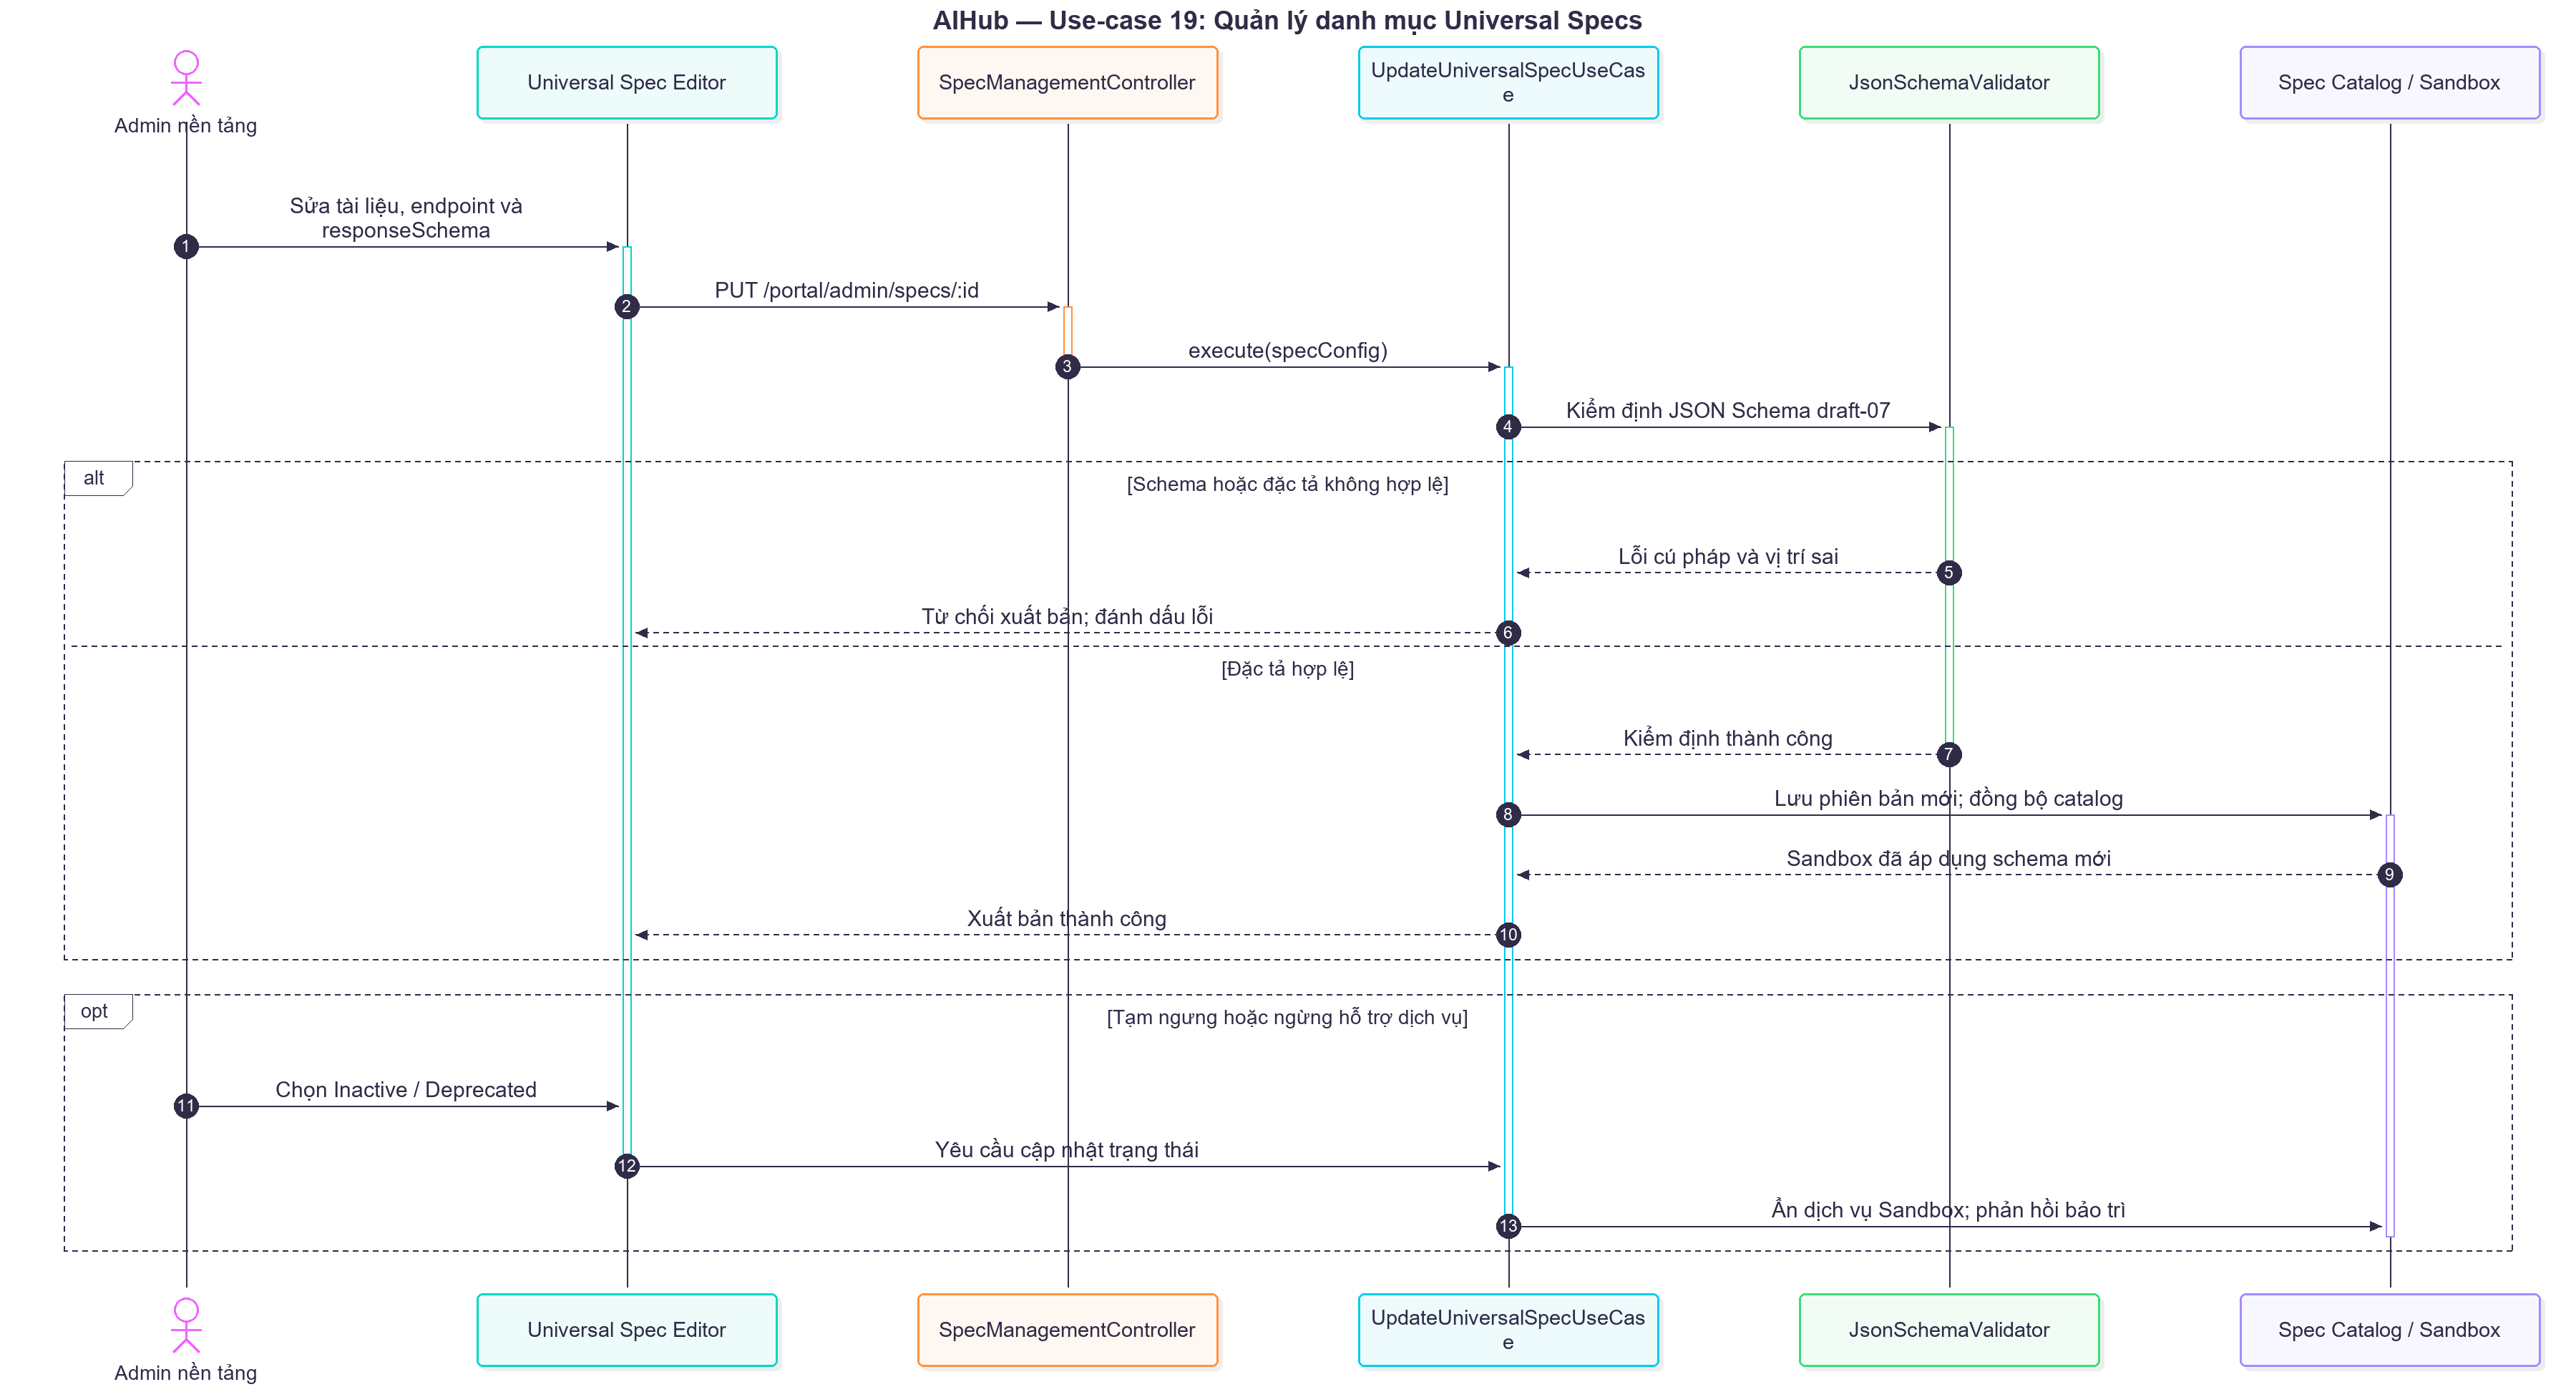
\includegraphics[width=\linewidth,height=.77\textheight,keepaspectratio]{Images/Sequence/AIHub/sequence_uc19_universal_specs.png}
\caption{Sequence diagram AIHub UC19 — Quản lý Universal Specs}
\label{sequence:aihub:sequence_uc19_universal_specs}
\end{figure}

Spec được version hóa và đồng bộ với Sandbox; phiên bản ngừng hoạt động không được sử dụng để chạy thử.

\clearpage
\paragraph*{UC20. Kiểm toán và truy vết giao dịch}

\begin{figure}[H]
\centering
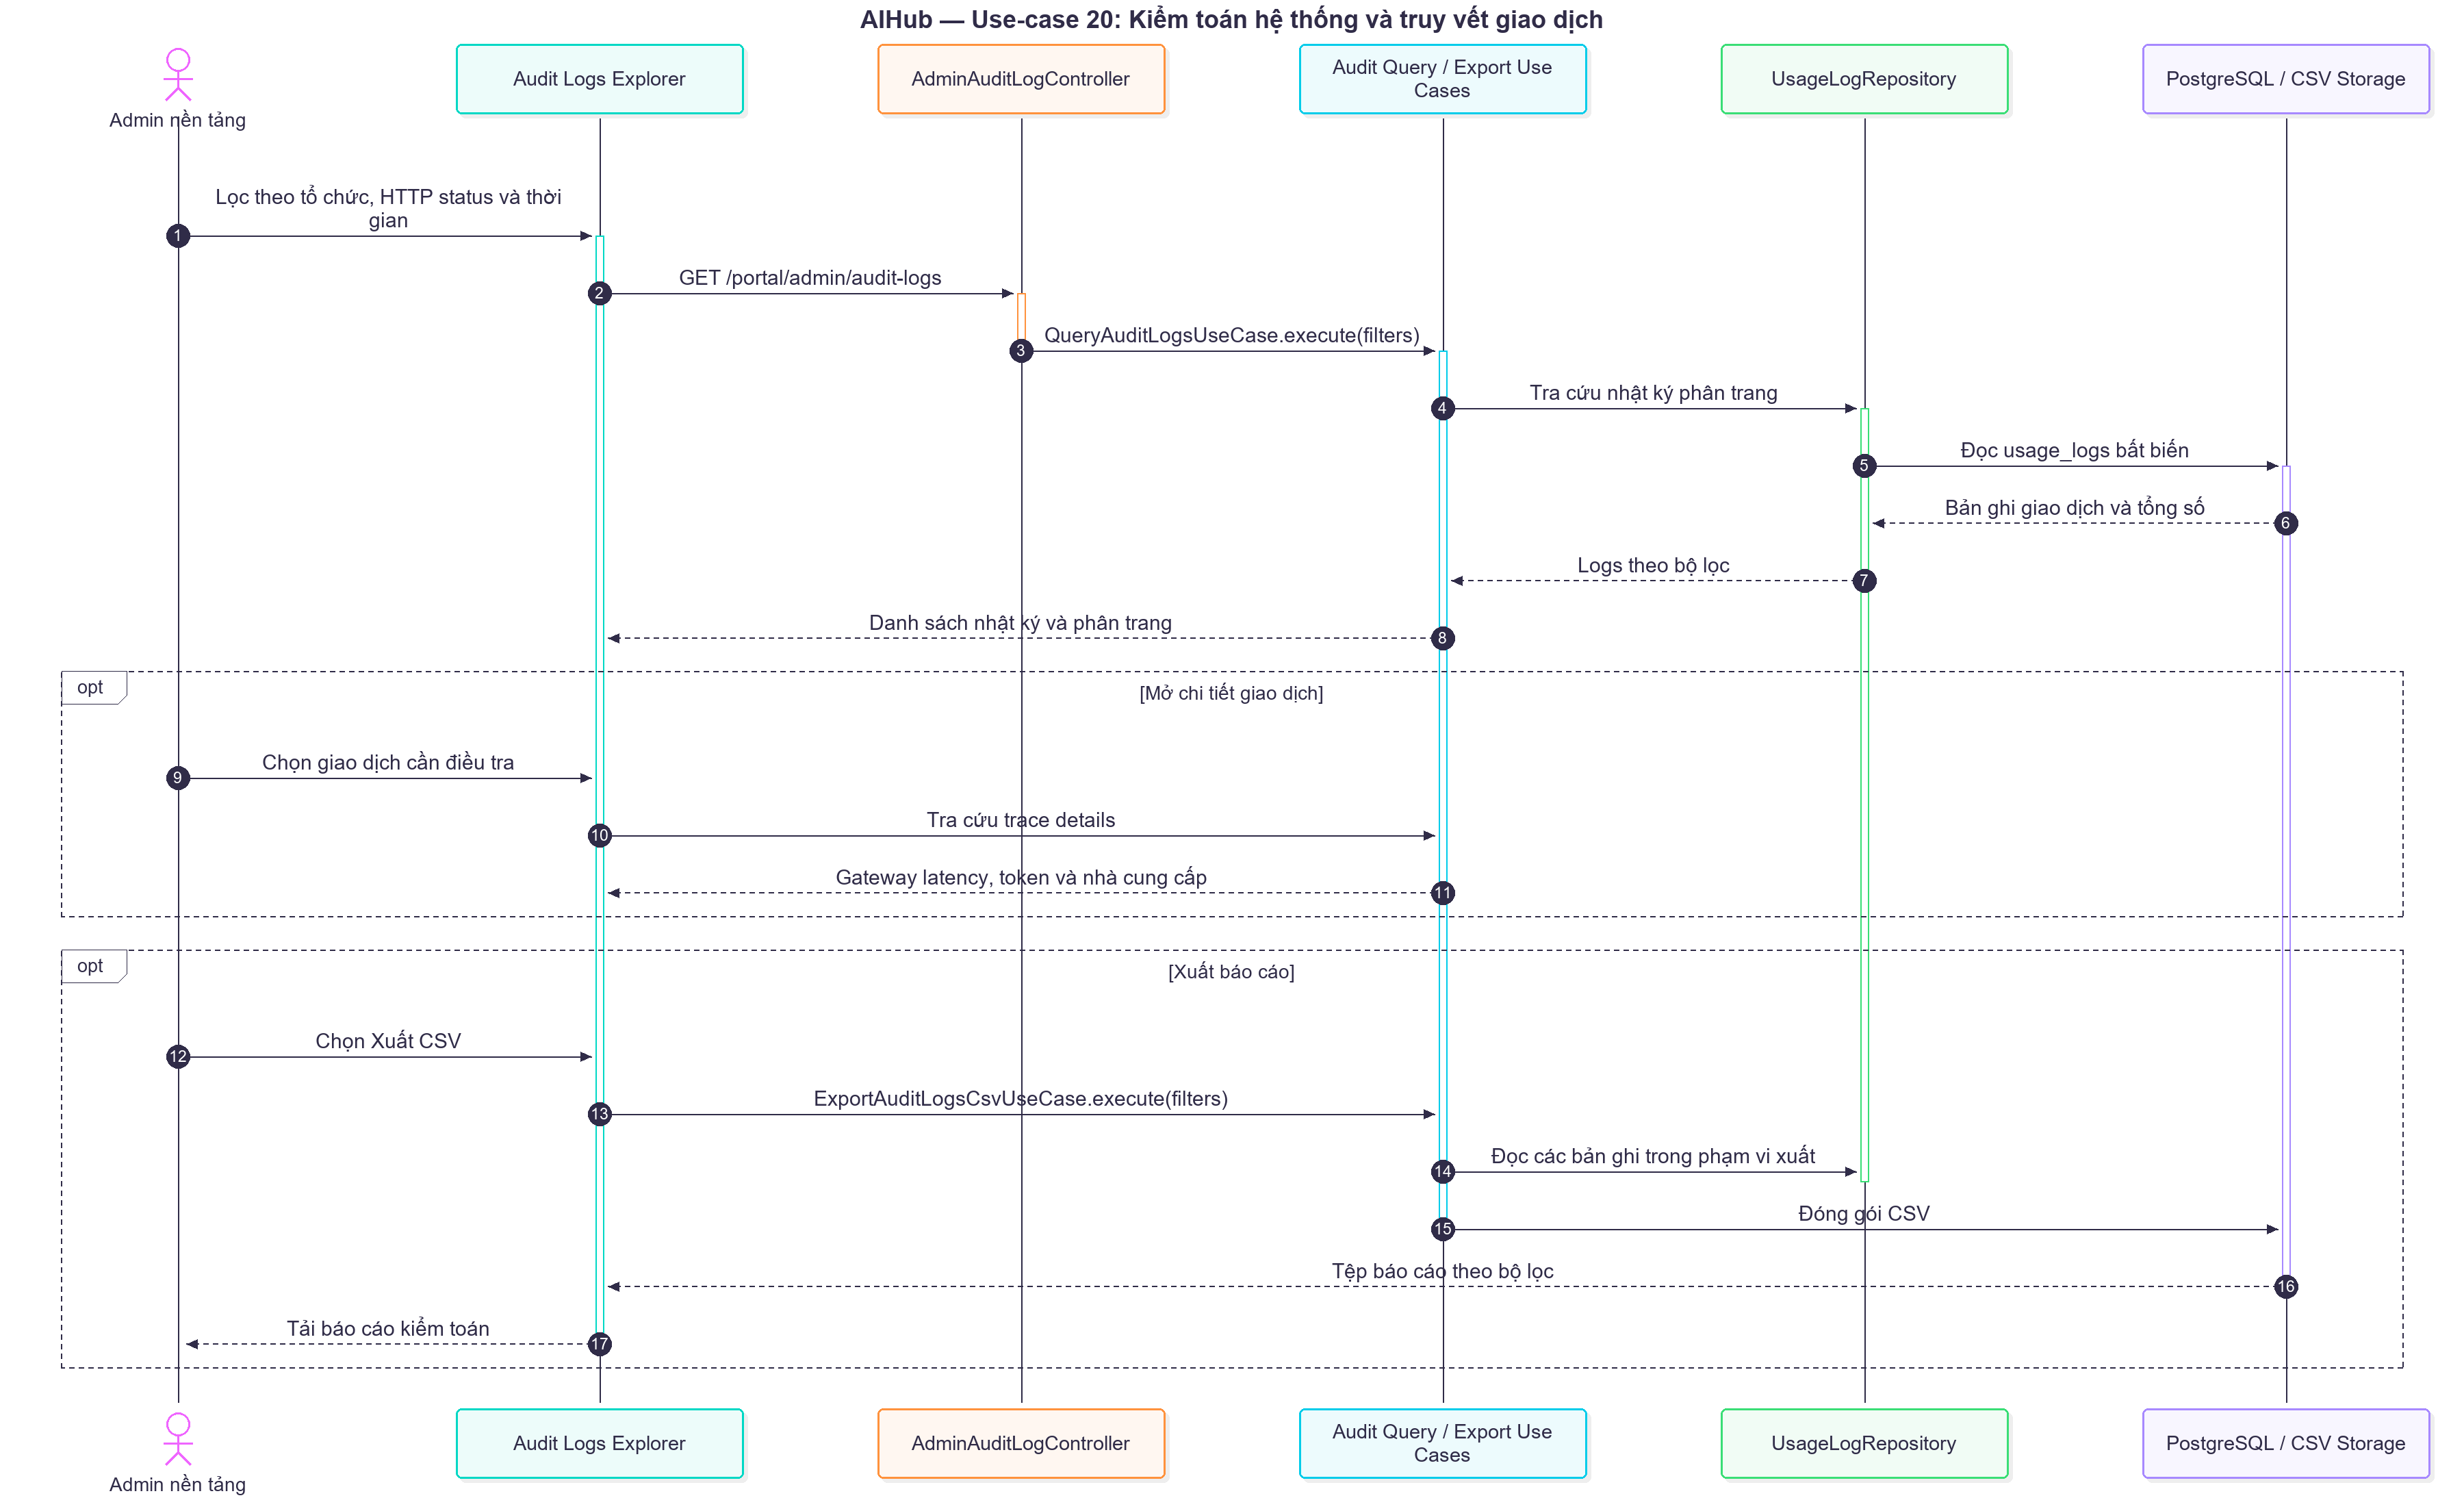
\includegraphics[width=\linewidth,height=.77\textheight,keepaspectratio]{Images/Sequence/AIHub/sequence_uc20_audit_logs.png}
\caption{Sequence diagram AIHub UC20 — Kiểm toán và truy vết giao dịch}
\label{sequence:aihub:sequence_uc20_audit_logs}
\end{figure}

Truy vấn và xuất dữ liệu áp dụng cùng phạm vi quyền; nhật ký không cung cấp thao tác sửa hoặc xóa trên Portal.

\subsubsection{Bảo mật và vận hành riêng của AIHub}

Gateway suy ra tổ chức từ credentials đã xác minh, sau đó kiểm tra quyền dịch vụ, trạng thái khóa và hạn mức. Portal sử dụng phiên người dùng; khóa B2B chỉ được cấp cho ứng dụng máy chủ của đối tác. Khu vực Academic Lab được kiểm tra bằng quyền nội bộ riêng tại từng endpoint.

B2B có hàng đợi \texttt{b2b.\allowbreak{}inference} và Academic Lab có hàng đợi \texttt{lab.\allowbreak{}generation}. Các tác vụ không được sử dụng hết tài nguyên GPU dành cho Wispace. Mọi thao tác cấp/thu hồi khóa, chuyển Owner, sửa gói, override quota, đổi model route và xuất dữ liệu đều cần audit. Khi công bố một dịch vụ, schema, phiên bản và quy tắc tính hạn mức phải được quản lý cùng nhau.

\subsection{Công nghệ, nguyên tắc tích hợp và triển khai}

\subsubsection{Kiến trúc vật lý và công nghệ}

Wispace và AIHub có frontend, backend .NET, Worker và cơ sở dữ liệu riêng. Hai hệ thống có thể áp dụng cùng bộ công nghệ và dùng hạ tầng vật lý chung trong phạm vi đồ án, nhưng được triển khai thành các dịch vụ độc lập. Việc chia sẻ máy chủ không cho phép truy cập chéo dữ liệu, phiên đăng nhập hoặc hạn mức.

\paragraph*{Lựa chọn mô hình kiến trúc}

Wispace được thiết kế theo microservices có chọn lọc: Core, Learning, Assessment, Reporting và AI Inference có khả năng phát hành và mở rộng độc lập. Nội bộ Core được chia module để giữ các nghiệp vụ nền tảng dễ quản lý. AIHub giữ kiến trúc \textbf{modular monolith} với API B2B, Portal và Academic Lab trong backend riêng. Sự khác biệt phản ánh nhu cầu phiên thi và suy luận của Wispace; không bắt buộc hai hệ thống có cùng mô hình triển khai \cite{ch7_microservices}.

Mỗi hệ thống có tiến trình .NET Worker và cấu hình hàng đợi riêng, triển khai từ bộ mã nguồn của backend tương ứng. API host tiếp nhận yêu cầu và tạo công việc; Worker xử lý công việc đã được ghi nhận. Worker là đơn vị triển khai riêng để yêu cầu HTTP có thể kết thúc sau khi nhận bài, còn việc chấm tiếp tục độc lập với kết nối của người dùng.

AI Runtime sử dụng Python FastAPI và được triển khai tách khỏi .NET. Hai hệ thống có thể gọi cùng dịch vụ suy luận đã được cấp quyền, bằng credentials và giới hạn tải riêng; đây là tích hợp dịch vụ AI, không phải dùng chung backend nghiệp vụ. Việc tách này cho phép sử dụng thư viện học máy, quản lý tài nguyên GPU và mở rộng năng lực suy luận theo nhu cầu. Trong từng module .NET, logic nghiệp vụ được tổ chức theo các lớp Domain, Application và Infrastructure; hướng phụ thuộc được quản lý thông qua interface và dependency injection \cite{ch7_dotnet_architecture}.

\begin{figure}[H]
\centering
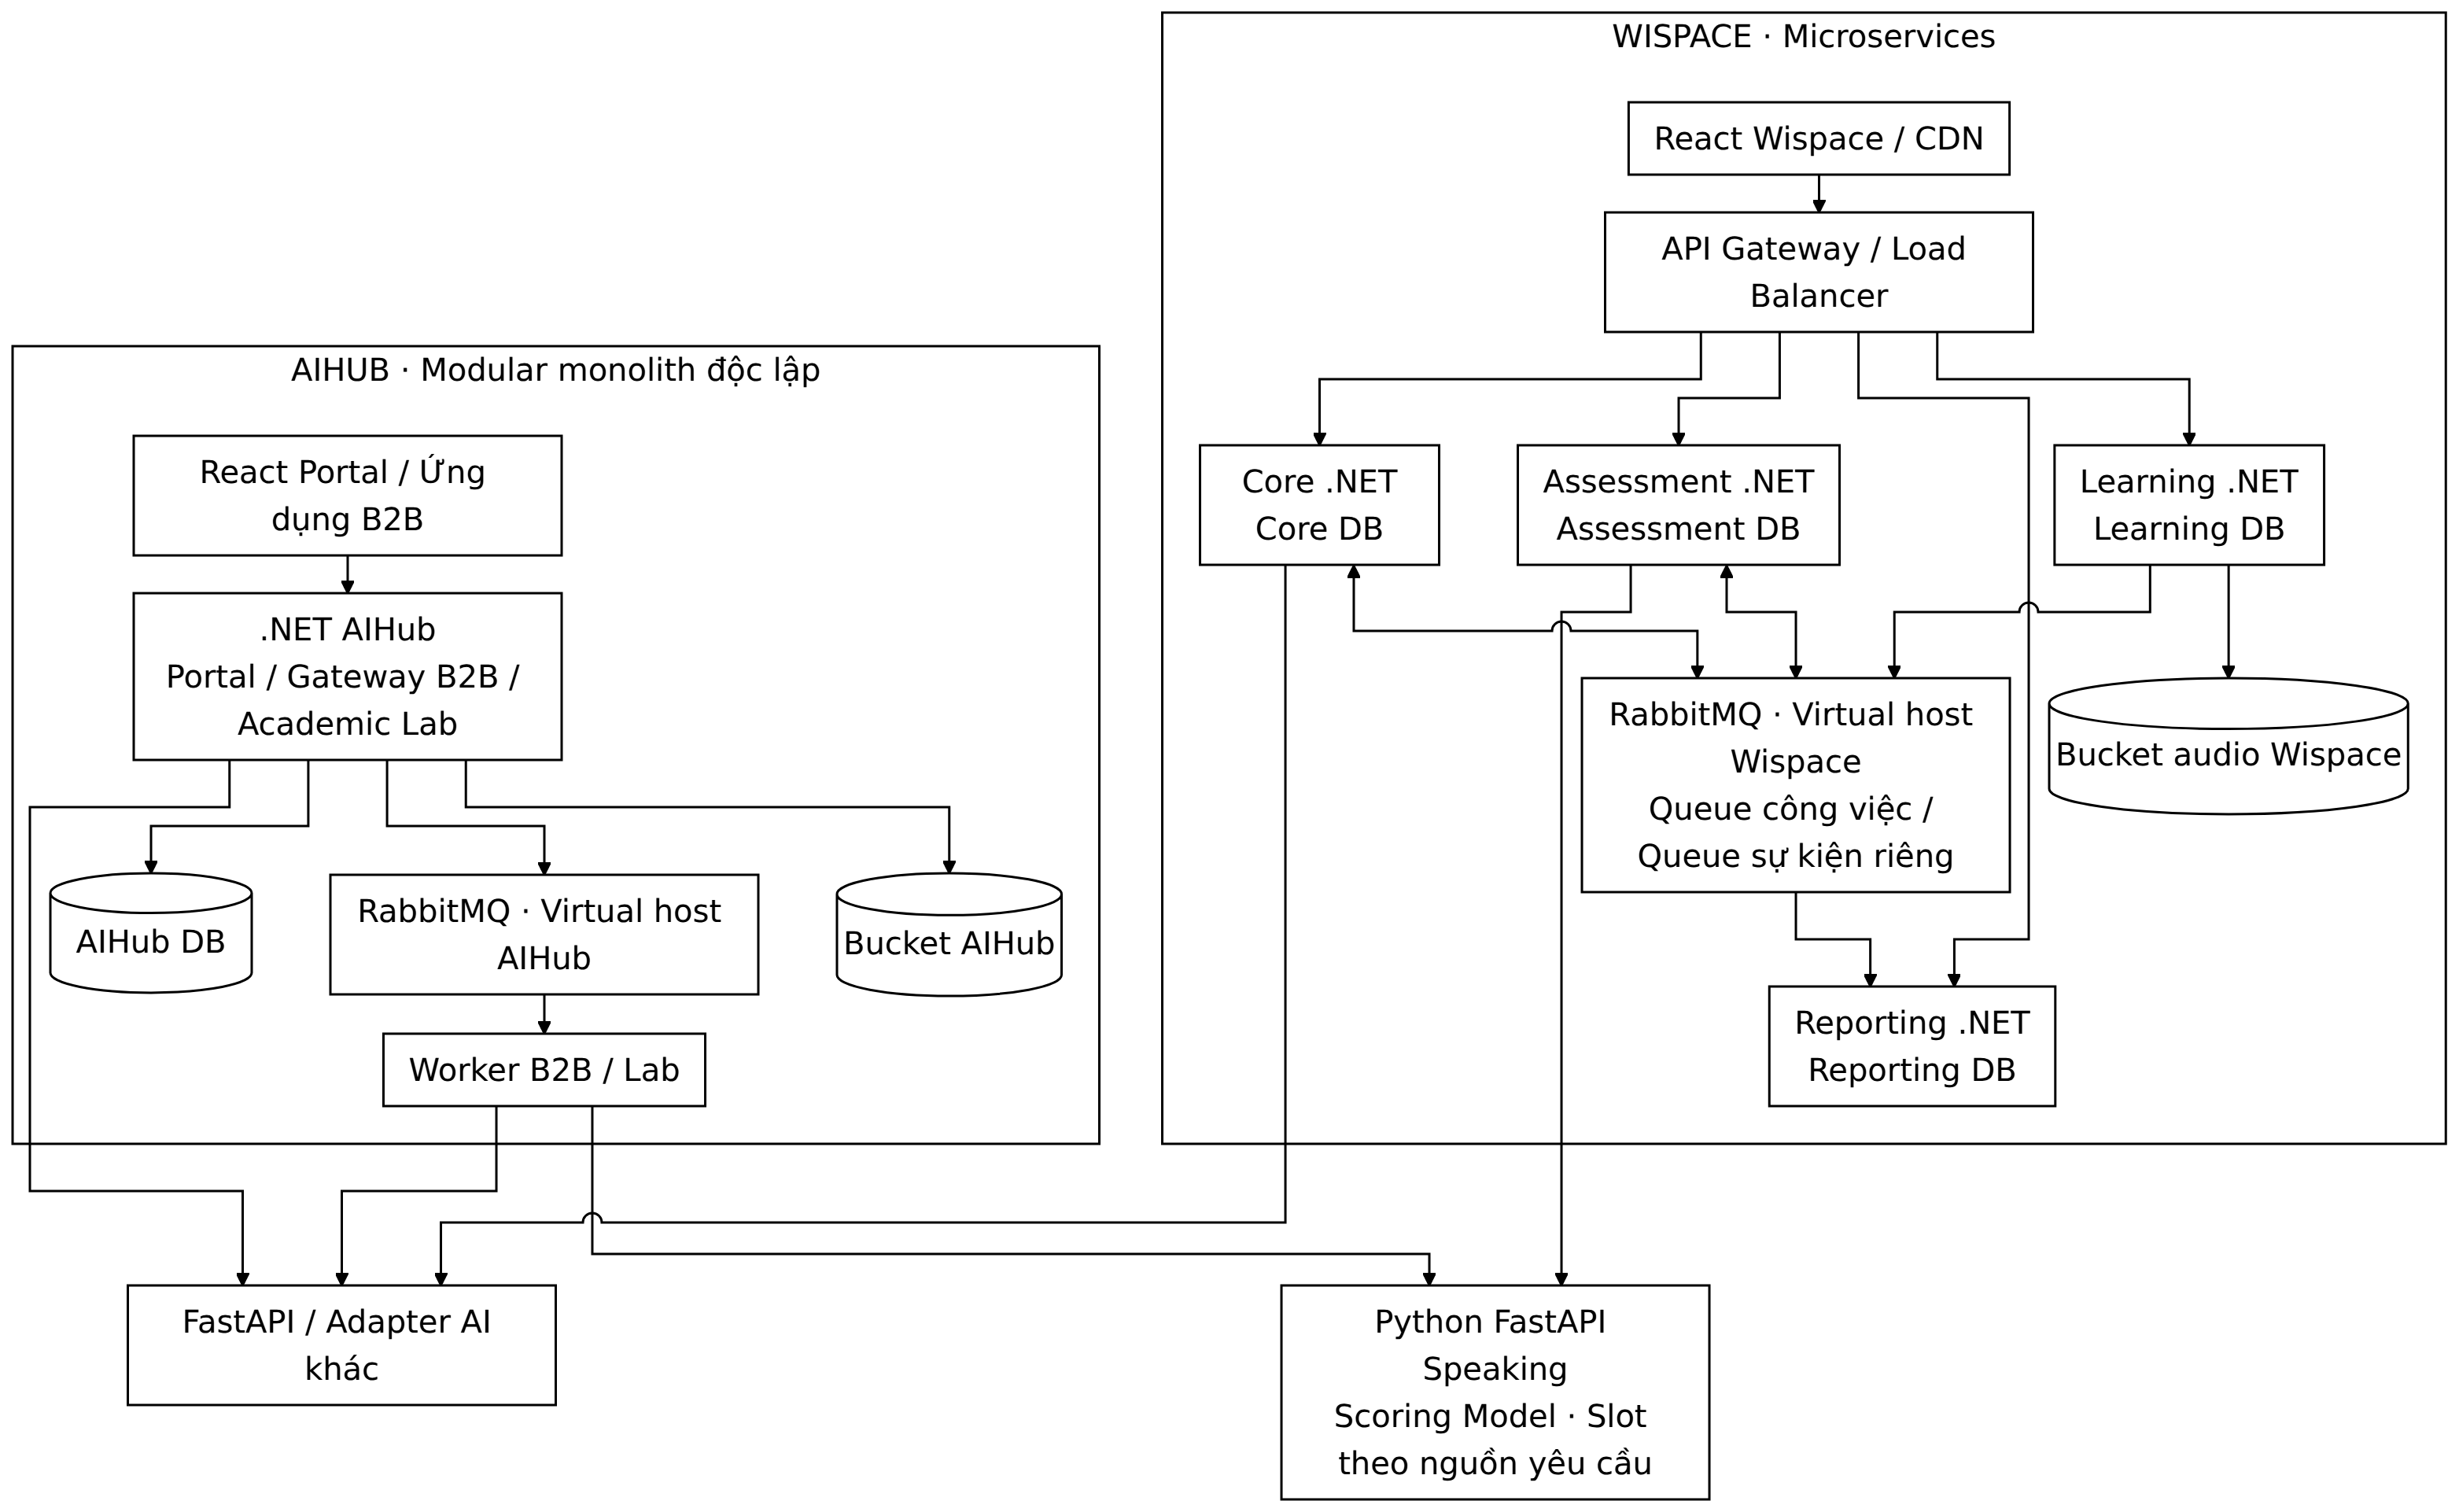
\includegraphics[width=\linewidth,height=.72\textheight,keepaspectratio]{Images/Design/shared_architecture.png}
\caption{Kiến trúc tổng thể hai hệ thống độc lập Wispace và AIHub}
\label{design:fig:shared_architecture}
\end{figure}

Sơ đồ biểu diễn các kênh xử lý chính. Khi Wispace cần tạo TTS hoặc thực hiện một tác vụ AI ngắn, Core hoặc dịch vụ Wispace được cấp quyền có thể gọi adapter FastAPI trực tiếp với timeout phù hợp. Đối với chấm bài và tác vụ dài, lời gọi được thực hiện bởi Worker thuộc luồng xử lý của Wispace. Luồng này không đi qua cổng API B2B của AIHub.

Đối tác chỉ truy cập các endpoint B2B công khai của .NET. FastAPI, RabbitMQ và PostgreSQL nằm trong mạng nội bộ. Frontend có thể truyền tệp trực tiếp đến Object Storage bằng quyền tải lên có thời hạn do backend cấp; các yêu cầu nghiệp vụ vẫn được xử lý qua .NET.

\paragraph*{Công nghệ đề xuất}

\begingroup\small\setstretch{1.1}
\begin{longtable}{|>{\raggedright\arraybackslash}p{\dimexpr 0.21\linewidth-2\tabcolsep-2\arrayrulewidth\relax}|>{\raggedright\arraybackslash}p{\dimexpr 0.35\linewidth-2\tabcolsep-2\arrayrulewidth\relax}|>{\raggedright\arraybackslash}p{\dimexpr 0.44\linewidth-2\tabcolsep-2\arrayrulewidth\relax}|}
\caption{Công nghệ đề xuất}\label{design:tab:3}\\
\hline
\textbf{Nhóm} & \textbf{Công nghệ} & \textbf{Mục đích} \\ \hline
\endfirsthead
\hline
\textbf{Nhóm} & \textbf{Công nghệ} & \textbf{Mục đích} \\ \hline
\endhead
\endfoot
Giao diện & React, TypeScript, Vite, React Router & Hai ứng dụng giao diện riêng; tổ chức route và màn hình theo nghiệp vụ. \\ \hline
Dữ liệu phía trình duyệt & TanStack Query & Quản lý dữ liệu lấy từ API, trạng thái tải và làm mới kết quả. \\ \hline
Backend & ASP.NET Core Web API & Cung cấp API, xác thực, phân quyền và xử lý nghiệp vụ theo module. \\ \hline
Truy cập dữ liệu & EF Core và Npgsql & Ánh xạ dữ liệu và thực hiện giao dịch trên PostgreSQL \cite{ch7_npgsql}. \\ \hline
Cơ sở dữ liệu & PostgreSQL & Nguồn dữ liệu chính cho tài khoản, bài làm, kết quả, hạn mức và cấu hình. \\ \hline
Tác vụ nền & .NET Worker / BackgroundService & Tiêu thụ công việc, gọi FastAPI và cập nhật kết quả. \\ \hline
Hàng đợi & RabbitMQ & Chuyển công việc giữa API host và Worker; xác nhận phát và xử lý thông điệp. \\ \hline
Lưu trữ tệp & Object Storage tương thích S3 & Lưu audio, tệp dữ liệu xuất và các tài nguyên mô hình ở vùng lưu trữ phù hợp. \\ \hline
AI & Python FastAPI và thư viện suy luận của Scoring Model & Đóng gói API suy luận, tiền xử lý âm thanh và các adapter AI. \\ \hline
Thông báo thời gian thực & ASP.NET Core SignalR & Thông báo tiến trình và kết quả; REST API vẫn cung cấp trạng thái có thể truy vấn lại. \\ \hline
Bộ nhớ đệm, khi cần mở rộng & Redis & Cache danh mục, cấu hình và trạng thái ngắn hạn; không thay thế dữ liệu nghiệp vụ trong PostgreSQL. \\ \hline
Triển khai & Docker Compose, reverse proxy Nginx & Đóng gói các thành phần và triển khai mô hình thử nghiệm của đồ án. \\ \hline
\end{longtable}
\endgroup

Phiên bản .NET, EF Core và Npgsql được chọn đồng bộ khi hiện thực. Các dependency React và Python được cố định bằng lockfile hoặc danh sách phiên bản để tái lập môi trường. Redis là thành phần mở rộng; bản triển khai ban đầu có thể sử dụng PostgreSQL cho các kiểm tra hạn mức và trạng thái để giảm số dịch vụ cần vận hành.

\subsubsection{Tổ chức lớp và giao dịch liên module}

Mỗi module chứa bốn nhóm thành phần:

\begin{itemize}
\item \textbf{API:} controller, xác thực request, DTO và ánh xạ lỗi HTTP.
\item \textbf{Application:} thực hiện ca sử dụng, kiểm tra quyền nghiệp vụ, điều phối giao dịch và gọi các interface tích hợp.
\item \textbf{Domain:} thực thể, trạng thái và các quy tắc như điều kiện nộp bài, quyền lợi gói hoặc vòng đời credentials.
\item \textbf{Infrastructure:} EF Core, PostgreSQL, RabbitMQ, Object Storage và HTTP client gọi FastAPI hoặc dịch vụ ngoài.
\end{itemize}

Domain không phụ thuộc trực tiếp EF Core hoặc SDK của nhà cung cấp AI. Các interface như \texttt{ISpeaking\allowbreak{}Scoring\allowbreak{}Client}, \texttt{IObject\allowbreak{}Storage}, \texttt{IQuota\allowbreak{}Service} và \texttt{IModel\allowbreak{}Provider} giúp thay thế cách tích hợp mà không thay đổi quy tắc nghiệp vụ.

\begin{figure}[H]
\centering
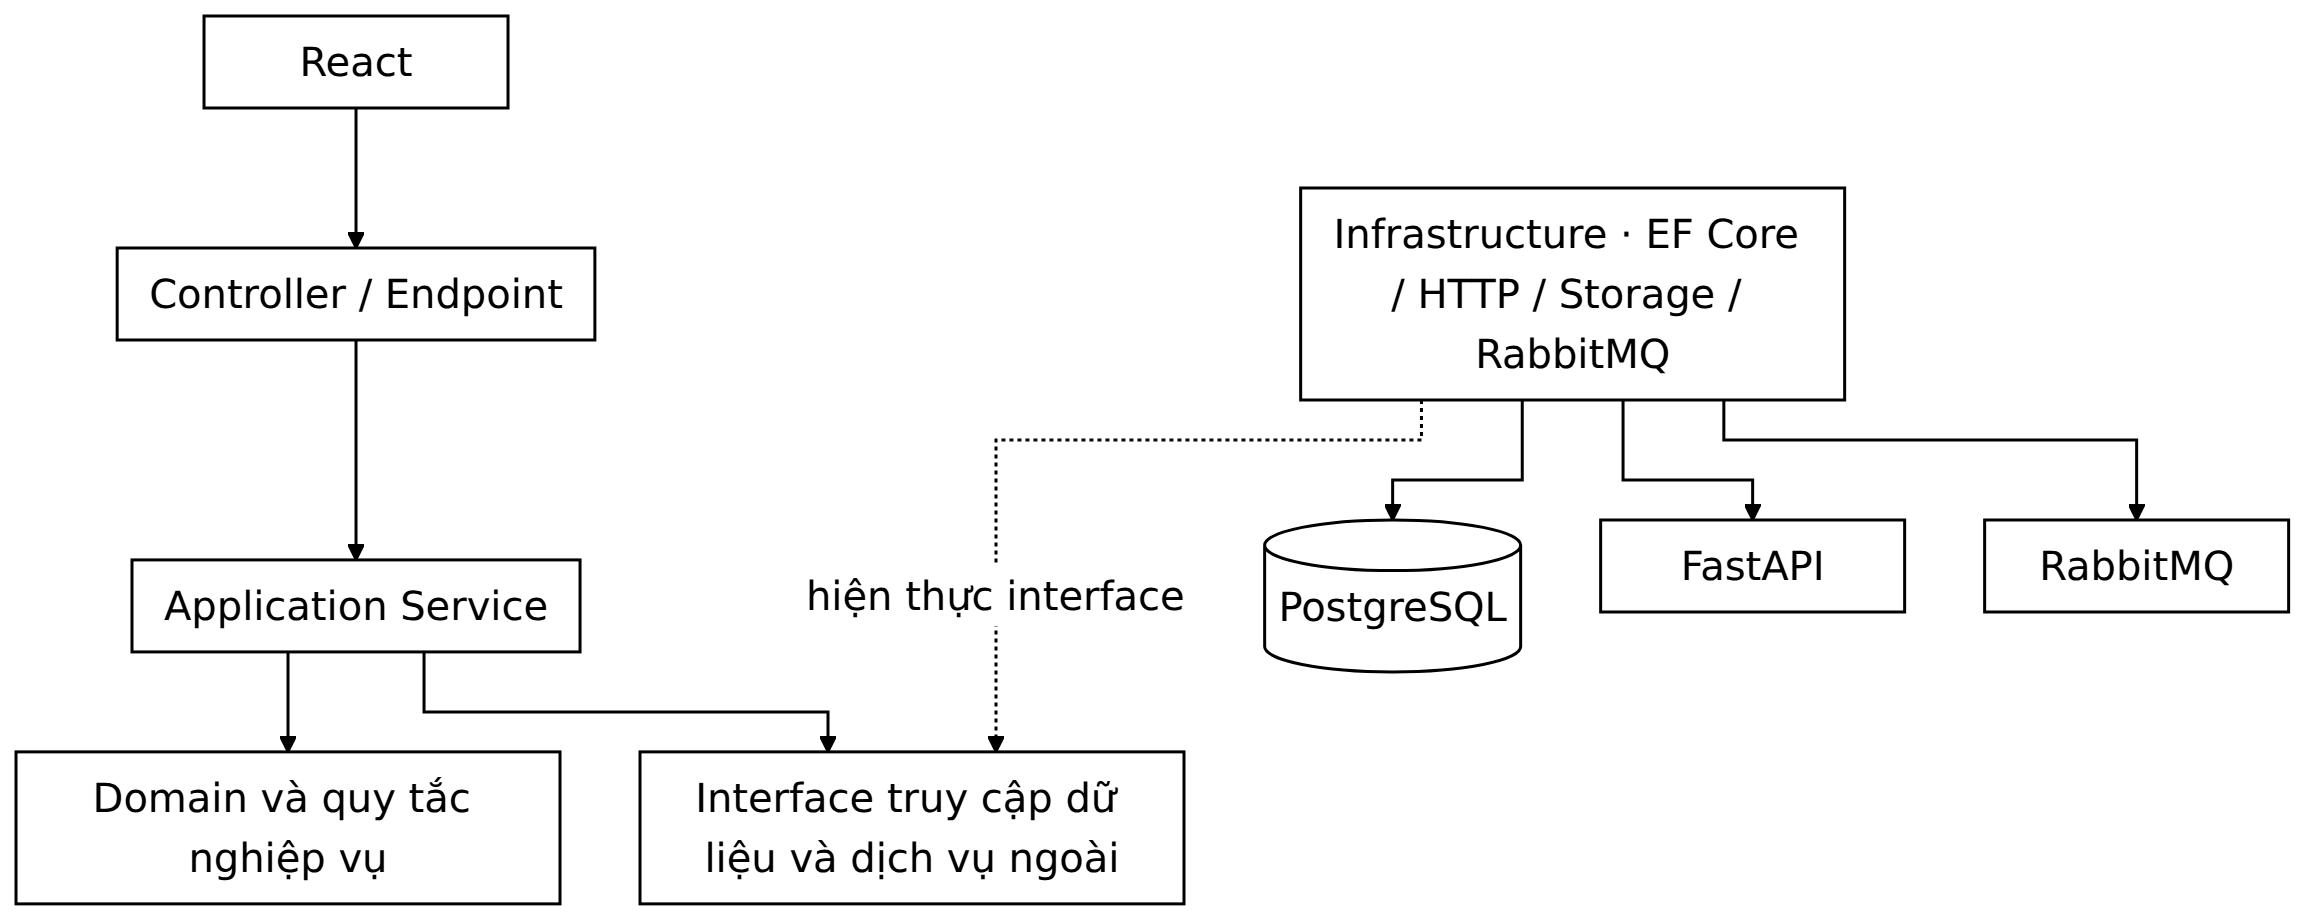
\includegraphics[width=\linewidth,height=.72\textheight,keepaspectratio]{Images/Design/module_layers.png}
\caption{Các lớp xử lý trong module .NET}
\label{design:fig:module_layers}
\end{figure}

Các mũi tên nét đứt trong sơ đồ biểu diễn quan hệ hiện thực interface. Ứng dụng kết nối các hiện thực cụ thể thông qua dependency injection khi khởi động.

Wispace dùng Core DB, Learning DB, Assessment DB và Reporting DB với quyền ghi và migration riêng. Core không sửa trực tiếp trạng thái job; Assessment không cập nhật sổ quota; Reporting không sửa dữ liệu nguồn. API đồng bộ được dùng cho truy vấn cần phản hồi ngay và giữ quyền lợi; sự kiện bất đồng bộ truyền kết quả và đồng bộ projection. Không duy trì transaction PostgreSQL hoặc khóa phân tán xuyên các dịch vụ trong lúc gọi mạng.

Trong Core, tài khoản/gói/quota có thể dùng transaction cục bộ qua hợp đồng module; trong AIHub, giao dịch B2B vẫn có thể dùng cùng connection của AIHub DB. Không áp dụng giả định transaction liên module này cho Learning, Core và Assessment đã tách biệt. Thay đổi hợp đồng cần tương thích phiên bản trong thời gian triển khai cuốn chiếu.

\subsubsection{Danh mục dữ liệu và ràng buộc nhất quán}

Bảng dưới đây mô tả các nhóm bảng, không phải một database dùng chung. Nhóm identity, question và billing của Wispace thuộc Core DB; session, answer và audio thuộc Learning DB; job, attempt, result và share thuộc Assessment DB; trend và roadmap thuộc Reporting DB. Mỗi dịch vụ có outbox/inbox và audit riêng. AIHub DB sở hữu identity của AIHub, aihub và lab; tên schema trùng nhau giữa các database không đồng nghĩa dùng chung danh tính.

\begingroup\small\setstretch{1.1}
\begin{longtable}{|>{\raggedright\arraybackslash}p{\dimexpr 0.13\linewidth-2\tabcolsep-2\arrayrulewidth\relax}|>{\raggedright\arraybackslash}p{\dimexpr 0.49\linewidth-2\tabcolsep-2\arrayrulewidth\relax}|>{\raggedright\arraybackslash}p{\dimexpr 0.38\linewidth-2\tabcolsep-2\arrayrulewidth\relax}|}
\caption{Danh mục dữ liệu và ràng buộc nhất quán}\label{design:tab:4}\\
\hline
\textbf{Schema} & \textbf{Nhóm bảng đề xuất} & \textbf{Nội dung chính} \\ \hline
\endfirsthead
\hline
\textbf{Schema} & \textbf{Nhóm bảng đề xuất} & \textbf{Nội dung chính} \\ \hline
\endhead
\endfoot
\texttt{identity} & \texttt{users}, \texttt{roles}, \texttt{user\_\allowbreak{}roles}, \texttt{sessions}, \texttt{refresh\_\allowbreak{}tokens}, \texttt{verification\_\allowbreak{}codes}, \texttt{consents} & Danh tính, phiên, xác minh và các lần đồng ý xử lý/sử dụng dữ liệu. \\ \hline
\texttt{core} & \texttt{question\_\allowbreak{}sets}, \texttt{questions}, \texttt{question\_\allowbreak{}audio}, \texttt{question\_\allowbreak{}submissions}, \texttt{question\_\allowbreak{}reports} & Kho đề và quy trình kiểm duyệt. \\ \hline
\texttt{learn\allowbreak{}ing} & \texttt{learning\_\allowbreak{}sessions}, \texttt{answers}, \texttt{audio\_\allowbreak{}assets} & Phiên học, câu trả lời, manifest audio và submission; job và attempt thuộc Assessment DB. \\ \hline
\texttt{assess\allowbreak{}ment} & \texttt{assessment\_\allowbreak{}results}, \texttt{criterion\_\allowbreak{}scores}, \texttt{detected\_\allowbreak{}errors}, \texttt{assessment\_\allowbreak{}jobs}, \texttt{assessment\_\allowbreak{}attempts}, \texttt{share\_\allowbreak{}links} & Job, attempt, kết quả, lỗi, báo cáo thi thử và link chia sẻ. \\ \hline
\texttt{report\allowbreak{}ing} & \texttt{progress\_projections}, \texttt{roadmap\_items}, \texttt{inbox\_events} & Tổng hợp lịch sử, xu hướng và roadmap từ sự kiện. \\ \hline
\texttt{billing} & \texttt{plans}, \texttt{plan\_\allowbreak{}entitlements}, \texttt{subscriptions}, \texttt{quota\_\allowbreak{}accounts}, \texttt{quota\_\allowbreak{}reservations}, \texttt{quota\_\allowbreak{}entries} & Gói Self-practice và sổ sử dụng hạn mức của học viên. \\ \hline
\texttt{billing} & \texttt{payment\_\allowbreak{}orders}, \texttt{payment\_\allowbreak{}events} & Đơn và thông báo thanh toán PayOS. \\ \hline
\texttt{aihub} & \texttt{organizations}, \texttt{organization\_\allowbreak{}members}, \texttt{api\_\allowbreak{}credentials}, \texttt{service\_\allowbreak{}catalog}, \texttt{model\_\allowbreak{}routes} & Khách hàng B2B, khóa và danh mục dịch vụ. \\ \hline
\texttt{aihub} & \texttt{organization\_\allowbreak{}plans}, \texttt{organization\_\allowbreak{}quota\_\allowbreak{}accounts}, \texttt{organization\_\allowbreak{}quota\_\allowbreak{}reservations}, \texttt{api\_\allowbreak{}requests}, \texttt{usage\_\allowbreak{}events} & Hạn mức và dữ liệu thực thi API của từng tổ chức. \\ \hline
\texttt{lab} & \texttt{references}, \texttt{samples}, \texttt{sample\_\allowbreak{}reviews}, \texttt{prompt\_\allowbreak{}versions}, \texttt{dataset\_\allowbreak{}exports}, \texttt{dataset\_\allowbreak{}export\_\allowbreak{}items} & Dẫn chứng, mẫu học thuật, thẩm định và xuất dữ liệu nội bộ. \\ \hline
\texttt{platform} & \texttt{model\_\allowbreak{}versions}, \texttt{file\_\allowbreak{}assets}, \texttt{outbox\_\allowbreak{}messages}, \texttt{audit\_\allowbreak{}events} & Phiên bản mô hình, tệp, sự kiện tích hợp và kiểm toán. \\ \hline
\end{longtable}
\endgroup

Các tên bảng là đề xuất phục vụ thiết kế. Hệ thống dùng khóa chính UUID cho các đối tượng có thể được truy cập qua API. Các thời điểm được lưu theo UTC; giao diện chuyển đổi theo múi giờ của người dùng. Dữ liệu có cấu trúc ổn định như điểm, trạng thái, chủ sở hữu và khóa ngoại được lưu bằng cột quan hệ. Metadata mở rộng của phản hồi AI có thể lưu bằng \texttt{jsonb} kèm phiên bản schema.

\begin{itemize}
\item Mỗi công việc chấm được định danh độc lập với từng lần thử. Kết quả cuối cùng có ràng buộc duy nhất theo \texttt{assessment\allowbreak{}Job\allowbreak{}Id}.
\item Một yêu cầu nộp có \texttt{Idempotency-\allowbreak{}Key} được ràng buộc theo người dùng, loại thao tác và mã yêu cầu; gửi lại cùng khóa không tạo thêm lượt chấm hoặc bút toán quota.
\item Sổ hạn mức có định danh nghiệp vụ duy nhất cho từng hành động giữ, tiêu thụ và hoàn. Số dư được kiểm tra và cập nhật trong transaction có khóa hoặc cập nhật có điều kiện.
\item Một thông báo PayOS được lưu với mã sự kiện duy nhất. Nhận lại cùng một thông báo không kích hoạt thêm thuê bao.
\item Các bản hiệu đính của Academic Lab sử dụng số phiên bản để phát hiện cập nhật đồng thời. \texttt{raw\allowbreak{}Ai\allowbreak{}Output} của mẫu gốc được bảo toàn.
\item Các bảng tổ chức B2B có \texttt{organization\allowbreak{}Id} và chỉ mục phục vụ lọc theo tổ chức. Những quan hệ cần cùng tenant được ràng buộc bằng khóa hoặc kiểm tra giao dịch tương ứng.
\end{itemize}

\subsubsection{Hợp đồng API và cập nhật trạng thái}

\paragraph*{Nhóm endpoint đề xuất}

\begingroup\small\setstretch{1.1}
\begin{longtable}{|>{\raggedright\arraybackslash}p{\dimexpr 0.21\linewidth-2\tabcolsep-2\arrayrulewidth\relax}|>{\raggedright\arraybackslash}p{\dimexpr 0.35\linewidth-2\tabcolsep-2\arrayrulewidth\relax}|>{\raggedright\arraybackslash}p{\dimexpr 0.44\linewidth-2\tabcolsep-2\arrayrulewidth\relax}|}
\caption{Nhóm endpoint đề xuất}\label{design:tab:5}\\
\hline
\textbf{Nhóm} & \textbf{Ví dụ endpoint} & \textbf{Trách nhiệm} \\ \hline
\endfirsthead
\hline
\textbf{Nhóm} & \textbf{Ví dụ endpoint} & \textbf{Trách nhiệm} \\ \hline
\endhead
\endfoot
Identity & \texttt{POST /\allowbreak{}api/\allowbreak{}v1/\allowbreak{}auth/\allowbreak{}login}, \texttt{POST /\allowbreak{}api/\allowbreak{}v1/\allowbreak{}auth/\allowbreak{}refresh} & Xác thực tài khoản và gia hạn phiên trình duyệt. \\ \hline
Kho đề Wispace & \texttt{GET /\allowbreak{}api/\allowbreak{}v1/\allowbreak{}wispace/\allowbreak{}questions} & Truy vấn đề theo quyền xem và bộ lọc. \\ \hline
Audio Wispace & \texttt{POST /\allowbreak{}api/\allowbreak{}v1/\allowbreak{}wispace/\allowbreak{}answers/\allowbreak{}\{id\}/\allowbreak{}uploads} & Tạo phiên tải audio và cấp quyền tải lên. \\ \hline
Hoàn tất audio & \texttt{POST /\allowbreak{}api/\allowbreak{}v1/\allowbreak{}wispace/\allowbreak{}uploads/\allowbreak{}\{id\}/\allowbreak{}complete} & Xác minh tệp hoặc các đoạn đã tải. \\ \hline
Nộp bài chấm & \texttt{POST /\allowbreak{}api/\allowbreak{}v1/\allowbreak{}wispace/\allowbreak{}answers/\allowbreak{}\{id\}/\allowbreak{}assessments} & Learning điều phối giữ quota tại Core, nhận submission và trả \texttt{202}; Assessment tạo job từ sự kiện. \\ \hline
Trạng thái nộp & \texttt{GET /\allowbreak{}api/\allowbreak{}v1/\allowbreak{}wispace/\allowbreak{}submissions/\allowbreak{}\{id\}} & Learning trả trạng thái tiếp nhận và các jobId đã được Assessment xác nhận; client chưa cần biết jobId khi nhận HTTP 202. \\ \hline
Kết quả & \texttt{GET /\allowbreak{}api/\allowbreak{}v1/\allowbreak{}wispace/\allowbreak{}assessments/\allowbreak{}\{id\}} & Trạng thái hoặc báo cáo theo quyền sở hữu. \\ \hline
Portal AIHub & \texttt{POST /\allowbreak{}api/\allowbreak{}v1/\allowbreak{}aihub/\allowbreak{}organizations/\allowbreak{}\{id\}/\allowbreak{}credentials} & Quản lý credentials theo quyền trong tổ chức. \\ \hline
API B2B & \texttt{POST /\allowbreak{}b2b/\allowbreak{}v1/\allowbreak{}services/\allowbreak{}\{service\allowbreak{}Code\}/\allowbreak{}requests} & Tiếp nhận yêu cầu đối tác và chọn cơ chế thực thi. \\ \hline
Trạng thái B2B & \texttt{GET /\allowbreak{}b2b/\allowbreak{}v1/\allowbreak{}requests/\allowbreak{}\{request\allowbreak{}Id\}} & Truy vấn yêu cầu thuộc tổ chức đã xác thực. \\ \hline
Academic Lab & \texttt{POST /\allowbreak{}api/\allowbreak{}v1/\allowbreak{}internal/\allowbreak{}lab/\allowbreak{}samples/\allowbreak{}\{id\}/\allowbreak{}reviews} & Ghi quyết định thẩm định của nhân sự nội bộ. \\ \hline
PayOS webhook & \texttt{POST /\allowbreak{}api/\allowbreak{}v1/\allowbreak{}payments/\allowbreak{}payos/\allowbreak{}webhook} & Xác minh thông báo thanh toán và cập nhật giao dịch. \\ \hline
AI nội bộ & \texttt{POST /\allowbreak{}internal/\allowbreak{}v1/\allowbreak{}speaking/\allowbreak{}assessments} & FastAPI thực thi một yêu cầu suy luận Speaking. \\ \hline
\end{longtable}
\endgroup

Các endpoint là hợp đồng đề xuất. API public của .NET, API B2B và API nội bộ của FastAPI được version hóa độc lập. Thay đổi schema không tương thích cần có phiên bản mới hoặc adapter chuyển đổi; không thay đổi ngầm phản hồi mà client đang sử dụng.

\paragraph*{Phản hồi và lỗi}

Lỗi trả về gồm mã lỗi nghiệp vụ, thông báo có thể hiển thị, \texttt{trace\allowbreak{}Id} và các trường không hợp lệ khi phù hợp. Không đưa stack trace, connection string, khóa bí mật hoặc URL audio riêng tư vào phản hồi lỗi.

Các mã HTTP được sử dụng nhất quán: \texttt{400} cho dữ liệu không hợp lệ, \texttt{401} cho thiếu hoặc sai xác thực, \texttt{403} cho thiếu quyền, \texttt{409} cho xung đột trạng thái hoặc idempotency, \texttt{429} cho giới hạn sử dụng và \texttt{503} khi dịch vụ tạm thời không sẵn sàng. Yêu cầu dài đã được chấp nhận trả \texttt{202}; mã này không biểu thị rằng việc chấm đã hoàn tất.

SignalR gửi các sự kiện như \texttt{Assessment\allowbreak{}Queued}, \texttt{Assessment\allowbreak{}Started}, \texttt{Assessment\allowbreak{}Completed} và \texttt{Assessment\allowbreak{}Failed} đến nhóm kết nối của đúng người dùng. Backend kiểm tra quyền khi đăng ký nhóm nhận thông báo. Thông báo chỉ chứa định danh và trạng thái cần thiết; frontend truy vấn REST API để lấy báo cáo đầy đủ.

Nếu mất kết nối SignalR, frontend tiếp tục truy vấn trạng thái theo chu kỳ với khoảng chờ tăng dần. Sau khi tải lại trang, trạng thái được khôi phục từ PostgreSQL thông qua API, thay vì dựa vào các thông báo đã nhận trước đó.

\subsubsection{Thiết kế bảo mật và quyền riêng tư}

\paragraph*{Tài khoản và phiên trình duyệt}

Backend sử dụng ASP.NET Core Identity cho tài khoản và các chức năng xác thực nền tảng \cite{ch7_aspnet_identity}. Đề xuất thống nhất hai frontend dùng access token thời hạn ngắn và refresh token trong cookie \texttt{Http\allowbreak{}Only}, \texttt{Secure}, với chính sách \texttt{Same\allowbreak{}Site} phù hợp cấu hình tên miền. Access token được giữ trong bộ nhớ của ứng dụng trình duyệt; refresh token được lưu dạng băm trên máy chủ, xoay vòng sau khi dùng và liên kết với phiên thiết bị.

Các endpoint dùng cookie, đặc biệt refresh và logout, phải có biện pháp chống CSRF, kiểm tra nguồn yêu cầu và cấu hình CORS theo đúng origin được phép. Tác vụ đăng xuất hoặc khóa tài khoản cập nhật trạng thái phiên trên máy chủ. API được bảo vệ kiểm tra trạng thái phiên và trạng thái tài khoản theo chính sách để việc thu hồi không chỉ phụ thuộc vào thời điểm JWT hết hạn.

Hai hệ thống quản lý danh tính, phiên đăng nhập và khóa xác thực độc lập. Cookie và token được giới hạn theo ứng dụng, issuer và audience; token Wispace không được chấp nhận tại AIHub. Quyền tổ chức B2B và quyền Academic Lab được kiểm tra trong backend AIHub. Thiết kế này chưa đặt yêu cầu đăng nhập một lần giữa hai hệ thống.

\paragraph*{Quyền sở hữu và phân tách dữ liệu}

Wispace kiểm tra \texttt{owner\allowbreak{}User\allowbreak{}Id} khi truy cập bài làm, audio và báo cáo riêng tư. Liên kết chia sẻ có mã ngẫu nhiên, phạm vi dữ liệu giới hạn và khả năng thu hồi; chỉ cho xem điểm và nhận xét theo yêu cầu, không tự cấp quyền nghe audio.

AIHub kiểm tra tư cách thành viên, vai trò và \texttt{organization\allowbreak{}Id} tại từng thao tác. Mã tổ chức trong URL phải khớp với phạm vi quyền đang có. Chỉ mục và các ràng buộc dữ liệu được thiết kế để tránh liên kết nhầm tài nguyên giữa hai tổ chức.

Các thao tác khóa tài khoản, đổi vai trò, cấp quota, thu hồi credentials, chuyển quyền tổ chức và xuất dữ liệu nội bộ đều ghi nhận kiểm toán. Audit event gồm tác nhân, phạm vi, loại thao tác, thời điểm, định danh đối tượng và lý do khi nghiệp vụ yêu cầu.

\paragraph*{Giao tiếp nội bộ và bảo vệ dữ liệu}

API nội bộ FastAPI chỉ được công bố trong mạng dịch vụ hoặc qua kết nối riêng có xác thực. Worker và các adapter .NET sử dụng service identity hoặc bí mật nội bộ được quản lý theo môi trường. Không dùng khóa B2B của khách hàng làm bí mật kết nối đến AI Runtime.

Backend kiểm tra định dạng, kích thước và quyền đối với audio trước khi xử lý. Nếu hỗ trợ URL đầu vào từ đối tác, hệ thống cần cơ chế nhập tệp có kiểm soát và giới hạn đích truy cập; bản đầu của đồ án nên ưu tiên upload qua quyền do backend cấp để tránh gọi tùy ý tới tài nguyên mạng nội bộ.

Nội dung đề và mẫu học thuật được xem là dữ liệu đầu vào của mô hình. Prompt hệ thống và quy tắc gọi dịch vụ do backend quản lý; văn bản do người dùng gửi không được dùng để thay đổi cấu hình nhà cung cấp hoặc trao quyền công cụ.

\paragraph*{Đồng ý sử dụng dữ liệu và chính sách xóa}

Hệ thống lưu riêng sự đồng ý xử lý audio để cung cấp dịch vụ và sự đồng ý sử dụng dữ liệu để huấn luyện. Việc chấp thuận điều khoản luyện tập không tự động được xem là chấp thuận huấn luyện. Khi xây dựng tập dữ liệu, bộ lọc xuất phải kiểm tra trạng thái đồng ý và các điều kiện sử dụng của từng mẫu.

Audio gốc, transcript, nhãn chuyên gia và dữ liệu dự đoán được phân biệt bằng nguồn gốc và phiên bản. Tập kiểm tra chuẩn được quản lý riêng để tránh sử dụng lại làm dữ liệu huấn luyện. Yêu cầu xóa tài khoản và dữ liệu được triển khai bằng quy trình có trạng thái, nhật ký và khả năng thử lại khi một hệ lưu trữ tạm thời gặp lỗi.

\subsubsection{Thiết kế triển khai và tài nguyên}

\paragraph*{Mô hình triển khai đề xuất}

Môi trường đồ án sử dụng Docker Compose cho các thành phần ứng dụng và dữ liệu. Hai frontend được build thành tài nguyên tĩnh, phục vụ qua reverse proxy. Wispace triển khai Core API, Learning API, Assessment API/Worker và Reporting API/Worker bằng các image riêng; FastAPI chạy trên nhóm máy GPU. AIHub API/Worker có image và lịch phát hành riêng. PostgreSQL có thể cùng cụm vật lý nhưng database và quyền truy cập tách theo dịch vụ; RabbitMQ dùng virtual host và credentials riêng cho Wispace/AIHub, với quyền exchange/queue phù hợp mỗi dịch vụ; Object Storage tách bucket và quyền theo nguồn dữ liệu. Docker Compose phục vụ phát triển và kiểm thử; production sử dụng nền tảng điều phối container nhiều máy hoặc cơ chế tương đương có health check, cân bằng tải, giới hạn tài nguyên và rolling deployment. Một máy chạy Compose không được xem là kiến trúc đáp ứng sẵn sàng cao cho tải mục tiêu.

Scoring Model được triển khai trên máy có GPU phù hợp; API host và PostgreSQL không phụ thuộc việc chạy chung máy GPU. Các dịch vụ AI khác có thể chạy trên CPU hoặc sử dụng nhà cung cấp ngoài tùy loại tác vụ. Docker Compose có thể tổ chức trên từng máy; việc kết nối máy GPU ở vị trí khác phải dùng mạng riêng hoặc kênh kết nối được bảo vệ.

\begin{figure}[H]
\centering
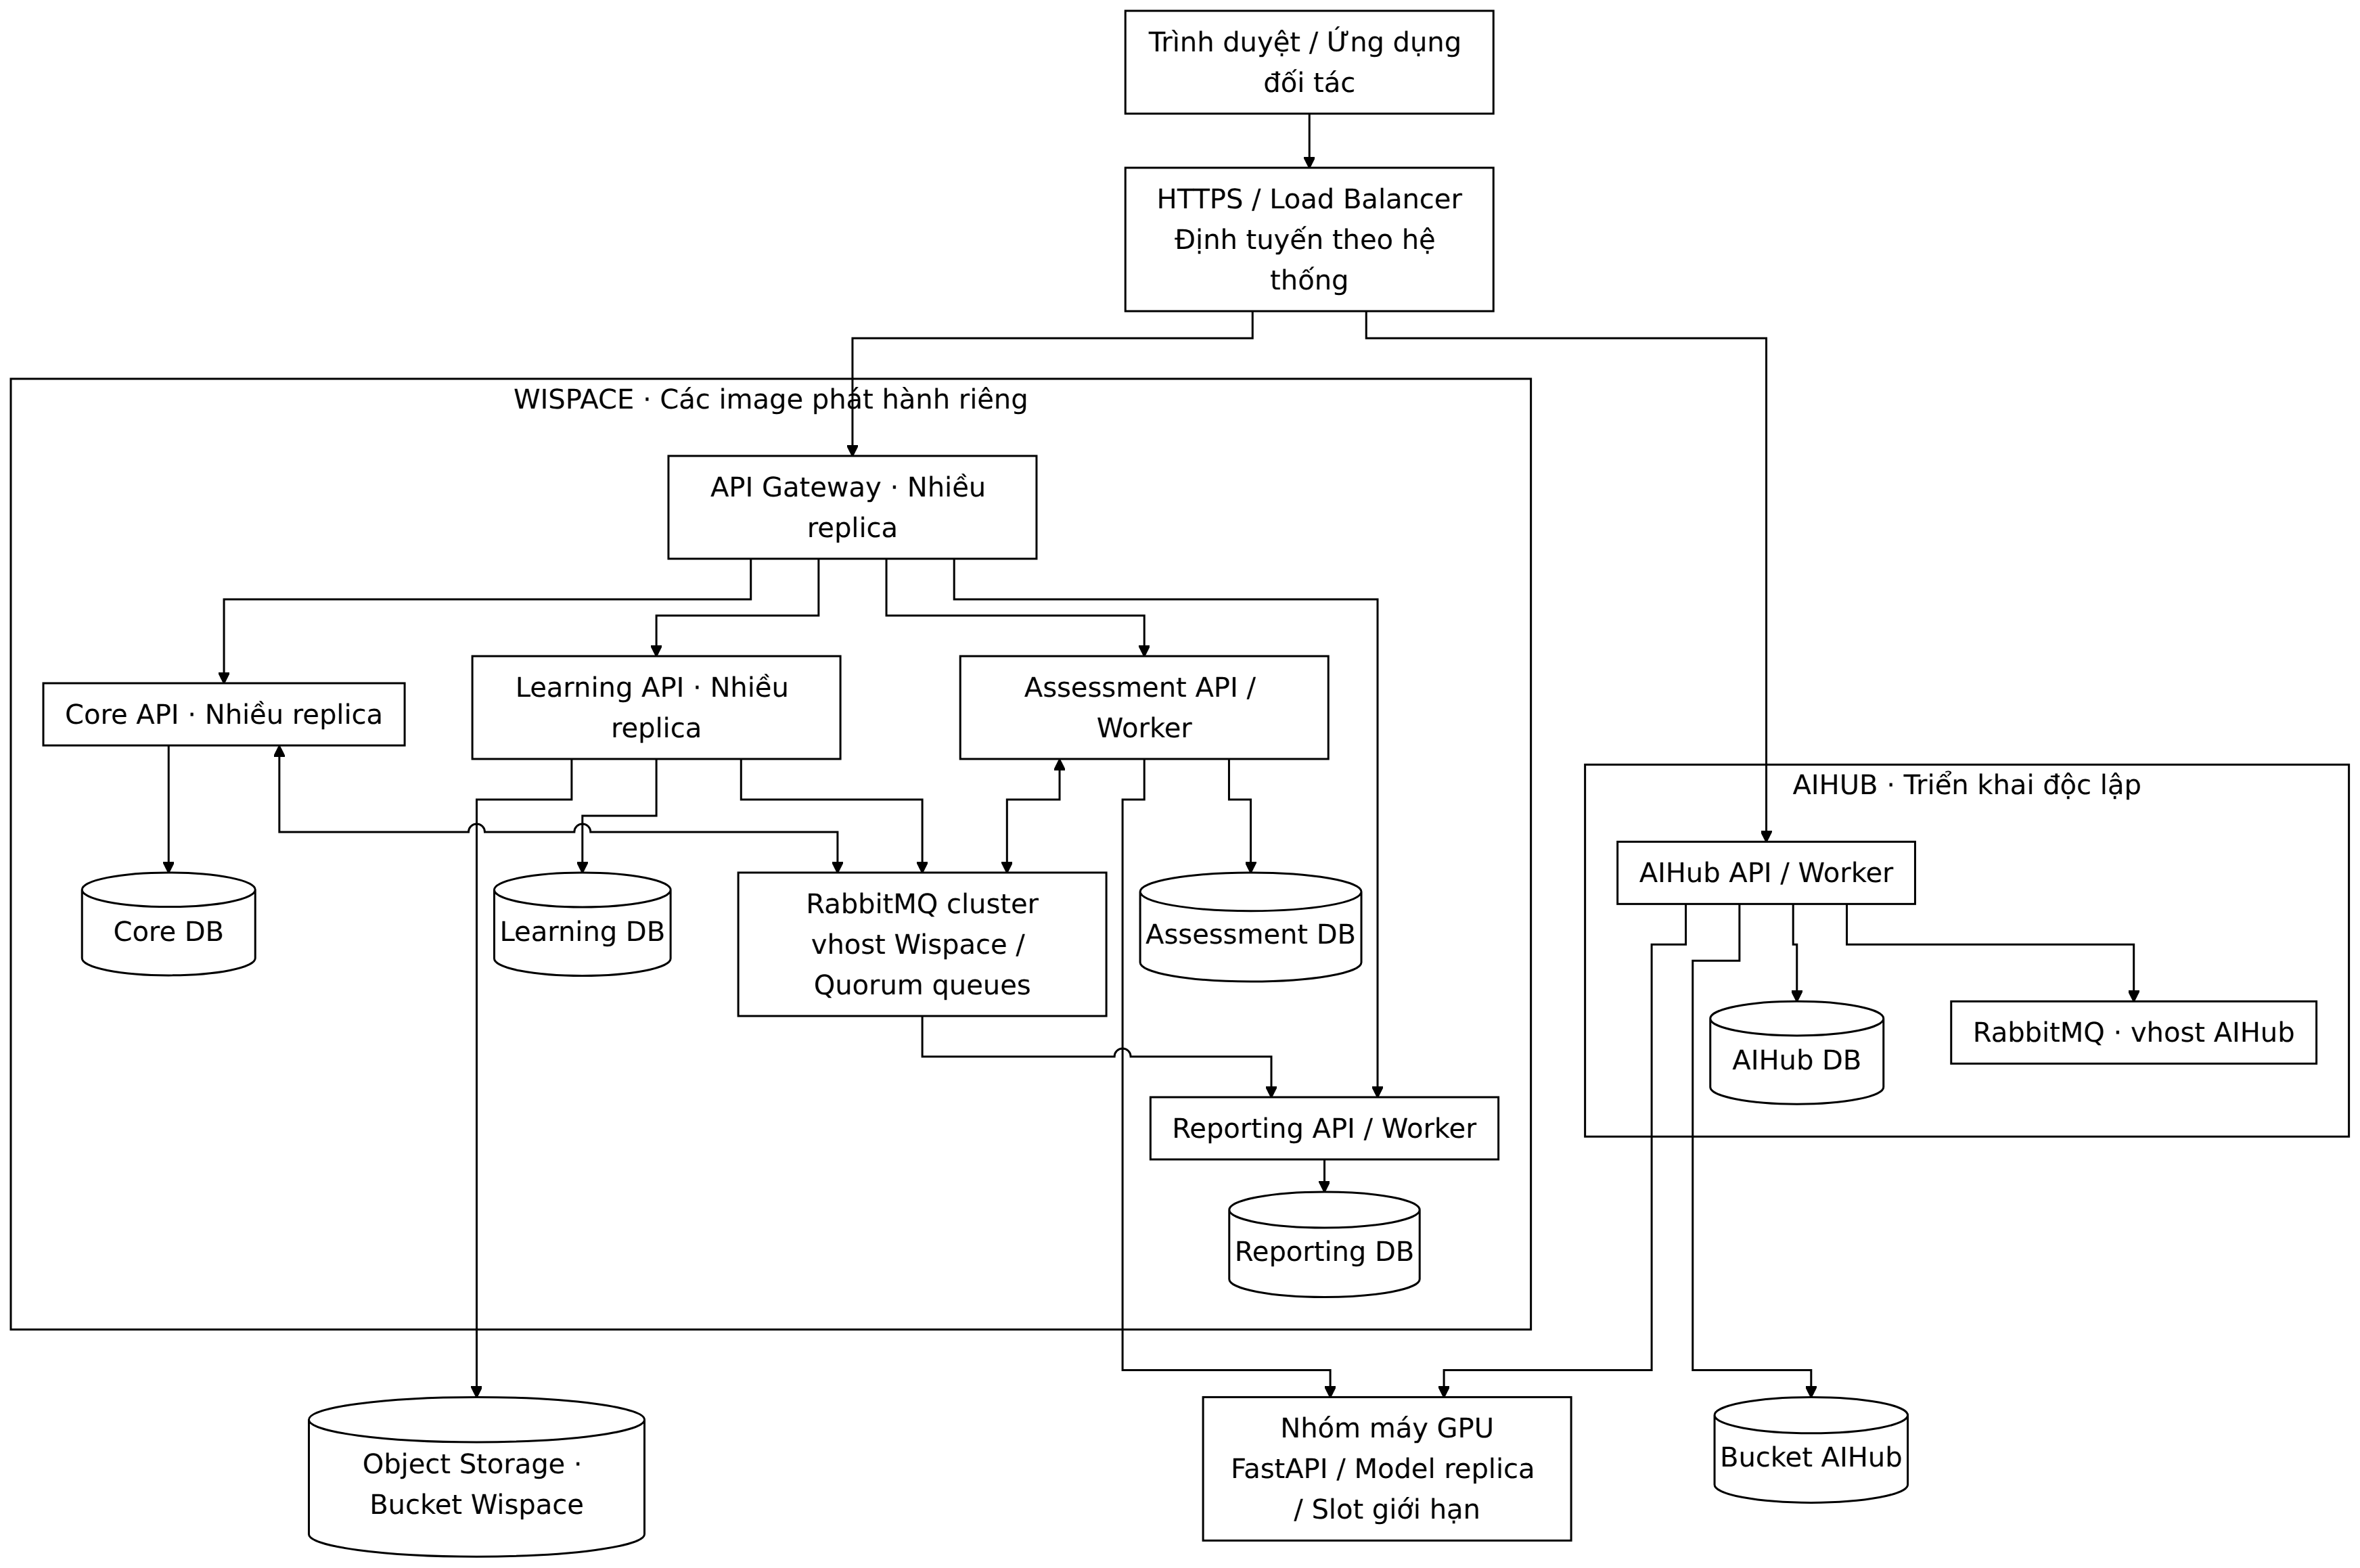
\includegraphics[width=\linewidth,height=.72\textheight,keepaspectratio]{Images/Design/deployment.png}
\caption{Mô hình triển khai ứng dụng và AI Runtime}
\label{design:fig:deployment}
\end{figure}

Việc đặt PostgreSQL và RabbitMQ cùng máy ứng dụng là lựa chọn cho môi trường thử nghiệm có quy mô nhỏ. Nếu máy này gặp sự cố, các thành phần cùng bị ảnh hưởng; bản triển khai đó chưa đủ để khẳng định đã đạt mục tiêu sẵn sàng hoặc chịu tải của Chương 5. Khi mở rộng, cơ sở dữ liệu, broker và ứng dụng có thể được triển khai trên các máy riêng hoặc dịch vụ được quản lý.

\paragraph*{Phân tách tải Wispace và B2B}

Các hàng đợi \texttt{speaking.\allowbreak{}assessment}, \texttt{b2b.\allowbreak{}inference} và \texttt{lab.\allowbreak{}generation} có cấu hình riêng về số Worker, prefetch và thời gian chờ. Các tác vụ Academic Lab hoặc đối tác không được sử dụng hết các slot suy luận dành cho lớp học và phiên thi đang hoạt động.

Khi dùng chung GPU, cần có cơ chế điều phối slot toàn cục ở lớp suy luận hoặc bộ lập lịch chung. Chỉ tách tên hàng đợi trong RabbitMQ chưa bảo đảm cô lập GPU. Trong bản triển khai đầu, có thể dành số slot cố định theo nhóm nguồn yêu cầu; số lượng cụ thể được xác định bằng thử nghiệm bộ nhớ và thời gian suy luận của mô hình.

Hệ thống giới hạn lượng công việc đang xử lý, theo dõi tuổi của công việc trong hàng đợi và áp dụng backpressure khi vượt ngưỡng. Mục tiêu mới là 1.000--10.000 người luyện/thi đồng thời; mức 200 phiên ở Chương 5 là kịch bản cơ sở cần nâng khi thống nhất yêu cầu. Kiểm thử lần lượt tải cơ sở, 1.000, 5.000 và 10.000 người theo tỷ lệ ghi âm/nộp bài thực tế, gồm đợt nộp đồng loạt và phục hồi kết nối. Đo p95/p99 API, lỗi, băng thông, connection pool, lock wait, tuổi công việc và thời gian chấm toàn luồng. Các mục tiêu 15 giây/câu, 3 phút/bài và 2 giây/chuyển câu vẫn là yêu cầu cần kiểm chứng; chưa có benchmark thì chưa thể cam kết số GPU, replica hoặc mức tải đạt được.

\paragraph*{Mở rộng API, dữ liệu và kết nối}

Core, Learning, Assessment API và Reporting API chạy stateless sau Gateway; trạng thái nghiệp vụ nằm trong database tương ứng. Redis có thể cache đề theo phiên bản, giới hạn tốc độ và dữ liệu đọc ngắn hạn; cache không quyết định bút toán quota. Truy vấn kết quả mới nhất đọc Assessment, còn biểu đồ xu hướng đọc Reporting và hiển thị thời điểm cập nhật khi projection chưa bắt kịp.

SignalR cần backplane hoặc dịch vụ quản lý kết nối khi chạy nhiều máy; cấu hình session affinity theo transport được sử dụng. Thông báo chỉ là tín hiệu để client đọc lại API nguồn; mất thông báo không làm mất kết quả. Tổng connection pool được giới hạn theo số replica và năng lực PostgreSQL, tránh tăng API gây cạn kết nối database. Hệ thống chia sẻ cấu hình xác thực/Data Protection phù hợp giữa các replica của cùng dịch vụ, dùng khóa dịch vụ và audience riêng khi giao tiếp nội bộ.

Autoscaling API dựa trên độ trễ, lưu lượng và tài nguyên; Worker dựa trên tuổi hàng đợi và năng lực GPU. Tăng Worker không được vượt tổng slot suy luận an toàn. Scale GPU cần tính thời gian nạp mô hình, bộ nhớ, độ dài audio và tỷ lệ retry. Admission control hạn chế mở phiên mới hoặc nhận chấm khi dự báo không đáp ứng được; không nhận vô hạn rồi xem việc lưu vào queue là đã đạt mục tiêu thời gian phản hồi.

\paragraph*{Cấu hình, backup và phát hành}

Connection string, bí mật OAuth, khóa PayOS và thông tin nhà cung cấp AI được cấu hình qua môi trường hoặc kho bí mật, tách khỏi Git. Mỗi môi trường có database, bucket, credentials và hạn mức riêng. FastAPI và các Worker có liveness/readiness probe phù hợp trạng thái kết nối và mô hình đã nạp.

PostgreSQL được backup định kỳ; bucket có chính sách bảo vệ và lưu trữ tương ứng. Quy trình khôi phục cần kiểm tra tính khớp giữa metadata trong database và object thực tế. Chỉ tạo được file backup chưa đủ để xác nhận có thể phục hồi toàn hệ thống.

Mỗi lần phát hành backend có bước kiểm tra migration trước khi đưa traffic vào. Mỗi phiên bản Scoring Model có artifact, checksum, cấu hình tiền xử lý và hợp đồng đầu ra tương ứng. Công việc đang chờ nên được gắn với phiên bản mô hình xác định, tránh thay đổi kết quả một cách khó truy vết khi chuyển phiên bản.

\subsubsection{Giám sát và xử lý sự cố}

\paragraph*{Dữ liệu quan sát hệ thống}

Mỗi yêu cầu có \texttt{trace\allowbreak{}Id} được truyền qua .NET, thông điệp RabbitMQ, Worker và FastAPI. Log có cấu trúc chứa định danh nghiệp vụ cần thiết nhưng không chứa bí mật xác thực, audio, URL ký trước hoặc toàn bộ nội dung nhạy cảm của người học.

Các nhóm chỉ số cần theo dõi gồm:

\begingroup\small\setstretch{1.1}
\begin{longtable}{|>{\raggedright\arraybackslash}p{\dimexpr 0.29\linewidth-2\tabcolsep-2\arrayrulewidth\relax}|>{\raggedright\arraybackslash}p{\dimexpr 0.71\linewidth-2\tabcolsep-2\arrayrulewidth\relax}|}
\caption{Dữ liệu quan sát hệ thống}\label{design:tab:6}\\
\hline
\textbf{Nhóm} & \textbf{Chỉ số chính} \\ \hline
\endfirsthead
\hline
\textbf{Nhóm} & \textbf{Chỉ số chính} \\ \hline
\endhead
\endfoot
API & Lưu lượng, thời gian đáp ứng, lỗi theo route, nguồn gọi và tổ chức. \\ \hline
Hàng đợi & Số công việc chờ, tuổi công việc, số đang chạy, số lần thử và công việc quá hạn. \\ \hline
Speaking & Thời gian chờ, tiền xử lý, suy luận, tỷ lệ lỗi audio và tỷ lệ job hoàn tất. \\ \hline
Mô hình/GPU & Phiên bản, bộ nhớ GPU, mức sử dụng, lỗi nạp mô hình và số slot khả dụng. \\ \hline
Nghiệp vụ & Lượt chấm, tỷ lệ hoàn quota, trạng thái thanh toán, mức sử dụng gói và chi phí ước tính. \\ \hline
Chất lượng & Sai lệch với nhãn chuyên gia, phân bố band, tỷ lệ thiếu tiêu chí và chất lượng theo nhóm dữ liệu. \\ \hline
\end{longtable}
\endgroup

Có thể bổ sung OpenTelemetry cho trace và metrics, cùng hệ thống hiển thị như Prometheus/Grafana khi cần. Bản đầu vẫn phải có log, định danh truy vết và các truy vấn vận hành cơ bản trước khi triển khai bộ dashboard đầy đủ.

\paragraph*{Chính sách xử lý sự cố}

\begingroup\small\setstretch{1.1}
\begin{longtable}{|>{\raggedright\arraybackslash}p{\dimexpr 0.29\linewidth-2\tabcolsep-2\arrayrulewidth\relax}|>{\raggedright\arraybackslash}p{\dimexpr 0.71\linewidth-2\tabcolsep-2\arrayrulewidth\relax}|}
\caption{Chính sách xử lý sự cố}\label{design:tab:7}\\
\hline
\textbf{Tình huống} & \textbf{Cách xử lý đề xuất} \\ \hline
\endfirsthead
\hline
\textbf{Tình huống} & \textbf{Cách xử lý đề xuất} \\ \hline
\endhead
\endfoot
RabbitMQ tạm thời không truy cập được & Giao dịch nhận bài và outbox đã ghi vẫn được giữ; Dispatcher thử phát lại. Theo dõi thời gian chưa phát để cảnh báo. \\ \hline
Worker dừng khi đang chấm & Lease hết hạn được phát hiện; công việc được khôi phục theo chính sách. Kết quả và quota có kiểm tra chống lặp. \\ \hline
Scoring Model quá tải & Giảm mức nhận việc, giữ job trong hàng đợi, ưu tiên slot Wispace và cập nhật trạng thái chờ. \\ \hline
Audio thiếu hoặc sai định dạng & Không chấm dữ liệu chưa đạt điều kiện; thông báo nguyên nhân, cho tải bù hoặc gửi lại khi phù hợp. \\ \hline
Phản hồi AI sai schema & Ghi lỗi hợp đồng, không lưu như kết quả hợp lệ; thử lại có giới hạn hoặc thất bại theo loại lỗi. \\ \hline
TTS lỗi & Dùng audio đã tạo trước hoặc nhà cung cấp TTS dự phòng đã cấu hình. \\ \hline
Object Storage lỗi & Giữ metadata ở trạng thái có thể khôi phục; không đánh dấu upload/xóa hoàn tất khi chưa xác nhận. \\ \hline
Redis lỗi & Dùng đường đọc PostgreSQL cho các chức năng được phép; chính sách giới hạn truy cập phải có hành vi dự phòng xác định. \\ \hline
PostgreSQL mất kết nối & Dừng nhận các thao tác cần đảm bảo nhất quán; không xác nhận đã giữ quota hoặc đã lưu kết quả khi chưa commit. \\ \hline
Callback thanh toán lặp & Xác minh và đối chiếu mã sự kiện; xử lý theo idempotency. \\ \hline
\end{longtable}
\endgroup

\paragraph*{Đánh giá và chuyển phiên bản mô hình}

Scoring Model mới được đánh giá trên bộ kiểm tra chuẩn không sử dụng để huấn luyện. Kết quả so sánh cần thể hiện sai lệch band, chất lượng theo tiêu chí, thời gian suy luận và khả năng xử lý dữ liệu của người học Việt Nam theo yêu cầu ở Chương 5.

Có thể chạy shadow trên một phần yêu cầu đủ điều kiện để so sánh phiên bản. Kết quả shadow không tiêu thụ thêm quota của người học và không tự ghi đè báo cáo chính. Khi phiên bản mới không đạt yêu cầu, model route được chuyển về phiên bản ổn định; mỗi kết quả đã lưu vẫn giữ phiên bản mô hình thực tế đã dùng.

\subsubsection{Kế hoạch hiện thực và thống nhất đặc tả}

\paragraph*{Thứ tự hiện thực đề xuất}

\begingroup\small\setstretch{1.1}
\begin{longtable}{|>{\raggedright\arraybackslash}p{\dimexpr 0.29\linewidth-2\tabcolsep-2\arrayrulewidth\relax}|>{\raggedright\arraybackslash}p{\dimexpr 0.71\linewidth-2\tabcolsep-2\arrayrulewidth\relax}|}
\caption{Thứ tự hiện thực đề xuất}\label{design:tab:8}\\
\hline
\textbf{Giai đoạn} & \textbf{Kết quả cần có} \\ \hline
\endfirsthead
\hline
\textbf{Giai đoạn} & \textbf{Kết quả cần có} \\ \hline
\endhead
\endfoot
1. Nền tảng và Wispace cơ bản & React Wispace, Core/Learning/Assessment/Reporting có dữ liệu riêng, Gateway, đăng nhập/phân quyền, kho đề, phiên thi và upload trực tiếp; AIHub có frontend và backend riêng. \\ \hline
2. Chấm Speaking và báo cáo & RabbitMQ, outbox, Worker, tích hợp Scoring Model, idempotency, quota, tiến trình và kết quả. \\ \hline
3. AIHub B2B & Tổ chức, credentials, danh mục API/mô hình, quyền dịch vụ, hạn mức, API đồng bộ/bất đồng bộ và usage. \\ \hline
4. Công cụ nội bộ và vận hành & Academic Lab, xuất dữ liệu có kiểm soát, giám sát, backup/restore, đánh giá mô hình và hoàn thiện phân tách tải. \\ \hline
\end{longtable}
\endgroup

Các giai đoạn là thứ tự đề xuất để triển khai đồ án, không phải trạng thái hiện thực đã được xác nhận. Các mục tiêu như độ lệch band, thời gian chấm và mức tải được kiểm thử sau khi có mô hình và môi trường chạy thực tế.

\paragraph*{Các điểm cần thống nhất khi đưa vào báo cáo chính}

\begingroup\small\setstretch{1.1}
\begin{longtable}{|>{\raggedright\arraybackslash}p{\dimexpr 0.29\linewidth-2\tabcolsep-2\arrayrulewidth\relax}|>{\raggedright\arraybackslash}p{\dimexpr 0.71\linewidth-2\tabcolsep-2\arrayrulewidth\relax}|}
\caption{Các điểm cần thống nhất khi đưa vào báo cáo chính}\label{design:tab:9}\\
\hline
\textbf{Nội dung} & \textbf{Cách thống nhất trong thiết kế này} \\ \hline
\endfirsthead
\hline
\textbf{Nội dung} & \textbf{Cách thống nhất trong thiết kế này} \\ \hline
\endhead
\endfoot
Vai trò của AIHub & Xác định AIHub là cổng quản lý/cung cấp API mô hình B2B; Academic Lab thuộc công cụ nội bộ. \\ \hline
Backend hai hệ thống & Wispace dùng microservices theo nhóm nghiệp vụ; AIHub dùng modular monolith riêng. Hai frontend, danh tính, hạn mức và triển khai độc lập. \\ \hline
Đường gọi AI Wispace & Assessment Worker của Wispace gọi trực tiếp FastAPI, không qua đường API B2B. \\ \hline
Xác thực Portal & Mỗi hệ thống xác thực riêng; thống nhất mô tả token và cookie trong đặc tả của từng hệ thống, không dùng chung phiên đăng nhập. \\ \hline
Số lần thử chấm & Trong thiết kế đề xuất: tối đa ba lần thực thi tự động, gồm một lần đầu và hai lần thử lại; sửa các chỗ dùng từ “retry” chưa cùng nghĩa khi đồng bộ Chương 5–6. \\ \hline
Hạn mức Speaking và B2B & Hai sổ hạn mức riêng theo người học và tổ chức; chi phí mô hình có thể được thống kê theo cùng nguồn tính toán. \\ \hline
Lưu trữ và quyền riêng tư & Audio riêng tư, link đọc tối đa 10 phút, xóa theo chính sách 180 ngày, đồng ý huấn luyện tách riêng đồng ý xử lý. \\ \hline
Mô hình chấm Speaking & Giữ giả định mô hình tự huấn luyện; chương thiết kế mô tả tích hợp và vận hành, không khẳng định chất lượng đã được thực nghiệm. \\ \hline
\end{longtable}
\endgroup

Chương này sử dụng thiết kế đề xuất Wispace–AIHub làm cơ sở hiện thực. Những điểm khác biệt so với các đặc tả ở Chương 5–6 được ghi rõ trong bảng trên để thống nhất khi triển khai; các mục tiêu hiệu năng và chất lượng cần được kiểm chứng bằng thực nghiệm.

\clearpage
\subsection{Kết chương}

Thiết kế đề xuất tổ chức Wispace và AIHub thành hai hệ thống độc lập, Wispace có frontend React và các microservice .NET với PostgreSQL sở hữu riêng; AIHub có frontend và backend modular monolith độc lập. Python FastAPI triển khai các năng lực AI theo hợp đồng dịch vụ. Wispace giữ vai trò sản phẩm học tập chính và gọi trực tiếp dịch vụ chấm Speaking; AIHub cung cấp cơ chế khai thác mô hình cho tổ chức B2B và các công cụ quản trị nội bộ.

Việc tách tác vụ chấm qua Worker và hàng đợi, quản lý audio bằng Object Storage, ghi nhận quota theo giao dịch và theo dõi phiên bản mô hình tạo cơ sở để hiện thực hệ thống có thể khôi phục và truy vết. Các thành phần triển khai, hợp đồng dữ liệu và chính sách vận hành trong chương là căn cứ cho quá trình xây dựng và đánh giá hệ thống ở các chương tiếp theo.

